\documentclass{book}
\usepackage{subcaption}
\usepackage{graphicx} % Required for inserting images
\usepackage[heading,UTF8]{ctex}             % 中文支持
\usepackage{geometry}                                       % 页面设置
\usepackage{fancyhdr,lastpage}                              % 页眉页脚
\usepackage{fontspec}                                       % 字体
\usepackage{tabularx,multirow,booktabs}                     % 表格
\usepackage{multicol}                                       % 分栏
\usepackage{listings}                                       % 代码
\usepackage{algorithm,algorithmicx,algpseudocode}           % 伪代码
\usepackage{amsmath,amsthm,amsfonts,amssymb,bm}             % 数学公式
\usepackage{epigraph}                                       % 引用
\usepackage{hyperref}                                       % 超链接
\usepackage{tikz}                                           % TikZ 画图
\usepackage{tcolorbox}                                      % Color Box
\usepackage{enumitem}                                       % 列表样式
\usepackage{xeCJKfntef,xcolor}                              % 文字加点
\usepackage{diagbox}
\usepackage{tasks}[=v1.3]
\usepackage{titlesec}
\usepackage{diagbox}
\usepackage{pifont}

\newcommand{\emptycell}{\rotatebox{160}{\rule{2em}{0.4pt}}} % 45度斜线
\newenvironment{problemtitle}
    {\centering\Large}

\hypersetup{                                                % 超链接样式
    colorlinks=true,
    linkcolor=black,
    filecolor=black,
    urlcolor=black,
    citecolor=black,
}

\usetikzlibrary{arrows.meta}                                % 附加箭头样式

\tikzset{                                                   % TikZ 设置
    global scale/.style={                                     % 整张图放缩
        scale=#1,
        every node/.append style={scale=#1}
    }
}

\tcbset{                                                    % Color Box 样式
    colback=white,
    colframe=black,
    boxrule=0.5pt
}

% \lstset{                                                    % 代码框格式设置
%     breaklines = true,
%     keepspaces = true,
%     basicstyle = \ttfamily,
%     numberstyle = \footnotesize\ttfamily\color{gray},
%     numbers = left,
%     columns = flexible,
%     framexleftmargin = 0pt,
%     xleftmargin = 12pt,
%     numbersep = 10pt,
%     keywordstyle = \color{black}, %\color{blue!70},
%     commentstyle = \color{black}, %\color{green!70},
%     frame = single,
%     frameround = tttt,
%     rulecolor = \color{blue},
%     language = c++,
%     escapeinside = {(*@}{@*)}
% }

% 样例的代码框格式设置 
\lstdefinestyle{sample} {
    breaklines = true,
    keepspaces = true,
    basicstyle = \ttfamily,
    numberstyle = \footnotesize\ttfamily\color{gray},
    % numbers = left,
    columns = flexible,
    framexleftmargin = 0pt,
    xleftmargin = 12pt,
    numbersep = 10pt,
    keywordstyle = \color{black}, %\color{blue!70},
    commentstyle = \color{black}, %\color{green!70},
    frame = single,
    frameround = tttt,
    rulecolor = \color{gray},
    framerule = 1pt,
    language = c++,
    escapeinside = {(*@}{@*)}
}

% pipipipipi43 需要的定义
\newcommand{\NormalTake}{\ensuremath{\bigtriangleup}}
\newcommand{\FreeTake}{\ensuremath{\bigcirc}}
\newcommand{\BadTake}{\ensuremath{\bigtriangledown}}
\newcommand{\DropTake}{\ensuremath{\bigstar}}
% 行内小标题
\newcommand{\idea}[1]{\par\medskip\noindent\textbf{#1}\quad}
\newtcolorbox{examplebox}[1]{
    colback=black!1,
    colframe=black!35,
    boxrule=0.5pt,
    arc=1.5pt,
    title=\textbf{#1},
    left=8pt,right=8pt,top=6pt,bottom=6pt
}
\newtcolorbox{infobox}{
    colback=white,
    colframe=black!35,
    boxrule=0.5pt,
    arc=1.5pt,
    left=8pt,right=8pt,top=6pt,bottom=6pt
}

\newtcolorbox{keybox}[1]{
    colback=black!2,
    colframe=black!55,
    boxrule=0.6pt,
    arc=1.5pt,
    title=\textbf{#1},
    colbacktitle=black!6,
    coltitle=black,
    left=8pt,right=8pt,top=6pt,bottom=6pt
}
\usetikzlibrary{arrows.meta,positioning,fit,calc}
% pipipipi43结束
% 标题别太松
\ctexset{
    section = {
        format = \centering\zihao{3}\bfseries\heiti,
        numbering = false,
        beforeskip = 0.5ex,
        afterskip = 1.2ex
    },
    subsection = {
        format = \large\bfseries\heiti,
        numbering = true,
        number = \chinese{subsection},
        aftername = {、\hspace{0.35em}},
        beforeskip = 1.0ex,
        afterskip = 0.8ex
    }
}

% 列表间距收紧
\setlist[itemize]{itemsep=2pt,topsep=4pt,parsep=0pt}
\setlist[enumerate]{itemsep=3pt,topsep=4pt,parsep=0pt}
\setlist[enumerate,1]{label=\arabic*.,leftmargin=2.2em}

% 公式上下别留太大空白
\setlength{\abovedisplayskip}{8pt}
\setlength{\belowdisplayskip}{8pt}
\setlength{\abovedisplayshortskip}{6pt}
\setlength{\belowdisplayshortskip}{6pt}

\definecolor{mygreen}{RGB}{0,128,0}
% 题解代码代码框格式设置
\lstdefinestyle{code}{
    breaklines = true,
    keepspaces = true,
    basicstyle = \ttfamily,
    numberstyle = \footnotesize\ttfamily\color{gray},
    keywordstyle = \color{blue!70}, 
    commentstyle = \color{gray}, 
    stringstyle = \color{mygreen},
    numbers = left,
    columns = flexible,
    framexleftmargin = 0pt,
    xleftmargin = 12pt,
    numbersep = 10pt,
    frame = L,
    frameround = tttt,
    framerule = 1pt,
    rulecolor = \color{gray},
    language = c++,
    escapeinside = {(*@}{@*)},
    showstringspaces = false
}
\xeCJKsetup{                                                % 文字下方加点样式
    underdot/symbol = {\color{black}.}
}

\newcommand{\filename}[1]{{\textbf{\textit{#1}}}}           % 自定义文件名样式
\newcommand{\myemph}[1]{{\textbf{\CJKunderdot{#1}}}}        % 自定义强调样式
\ctexset{                                                   % 标题设置
    section = {
        format = \centering\Large\heiti,
        numbering = true,
        number = {},
        aftername = {}
    },
    subsection = {
        format = \fontsize{13pt}{\baselineskip}\heiti,
        numbering = true,
        number = \chinese{subsection},
        aftername = {、},
        % aftertitle = {】}
    },
    subsubsection = {
        format = \myemph,
        numbering = true,
        number = {},
        aftername = {【},
        aftertitle = {】}
    }
}

\geometry{                                                  % 页面设置
    a4paper,
    left = 70pt,
    right = 70pt,
    top = 80pt,
    bottom = 65pt,
    footskip = 30pt
}

\floatname{algorithm}{算法}
\renewcommand{\algorithmicrequire}{\textbf{输入：}}
\renewcommand{\algorithmicensure}{\textbf{输出：}}

\setmonofont{Consolas} [
    Path = ./, 
    Extension = .ttf,
]              % 等宽字体

\usepackage{xcolor}  % 处理` ` 问题
\definecolor{codebg}{rgb}{0.95,0.95,0.95}  % 浅灰色背景

\newcommand{\code}[1]{\colorbox{codebg}{\texttt{#1}}}  % 带背景色的代码

    
\setlist[itemize]{itemsep=0pt,partopsep=0pt,parsep=0pt,topsep=10pt}
\setlist[enumerate]{itemsep=0pt,partopsep=0pt,parsep=0pt,topsep=10pt}
\setlist[itemize,1]{leftmargin=35pt}
\setlist[enumerate,1]{leftmargin=35pt}

\newcommand{\docTitle}{CSP-S初赛解析}
\newcommand{\docSecTitle}{}
\newcommand{\docThiTitle}{}
\newcommand{\docAuthor}{}
\newcommand{\docDate}{年月日 $\sim$ }

\newcommand{\fancyheadLeftText}{\docTitle}
\newcommand{\fancyheadRightText}{\docThiTitle}

\title{\docTitle}
\author{\docAuthor}
\date{\docDate}

\hypersetup{
    pdftitle={\docTitle},
    pdfauthor={\docAuthor}
}

\makeatletter
\renewcommand*\maketitle{                                   % 标题页格式设置
    \begin{center}
        {\LARGE \bfseries \@title \par}
        {\Huge \heiti \docSecTitle \par}
        {\LARGE \kaishu \docThiTitle \par}
        {\large \@author \par}
        {\large \heiti 时间：\@date \par}
    \end{center}
    \setcounter{footnote}{0}
}
\makeatother


\setcounter{tocdepth}{1} 

\setlist[enumerate,1]{
  itemsep = 30pt,
  label=\arabic*.,    % 标签格式为 1. 2. 3.
  leftmargin=*,       % 左对齐
  % resume              % 自动连续编号（如果分段）
}
\setlist[enumerate,2]{
  label=\Alph*.,    % 标签格式为 A. B. C.
  leftmargin = 24pt
}

\settasks{
    label = {\Alph*.}, % A, B, C, ...
    label-width = 15pt
    
}


\pagestyle{fancy}
\fancyhf{} % 清空默认设置
\fancyfoot[RO]{\thepage} % 奇数页页码在右
\fancyfoot[LE]{\thepage} % 偶数页页码在左
\renewcommand{\headrulewidth}{0pt} % 去掉页眉横线


\begin{document}



\frontmatter

\chapter{序}
    随着各位同学努力的学习，终于到了冲刺提高组奖项的时刻。或许你是刚巩固完入门组知识点，正准备学习提高组内容；或许你已经学完了提高组的知识点，正在大量刷题备赛；或许你已经有了提高组的奖项，但你想要冲刺更高的目标和奖项。无论你处于什么环节，我希望这本书都能对你有一定的帮助。
\section*{这是一本什么书？}
    这是一本你可以随身携带的《小》“字典”（我们本来真的打算少写点，写着写着就300多页了(逃)）。随着年级的不断增长，大家平时能使用电脑的时间也会越来越少。但是提高组的难度更高，内容也更多，难免会有一些东西忘记。因此我们准备了这个字典，你可以用它来进行日常的复习，也可以在你忘记某个知识点时翻出这本书快速地查询。
    
    这也是一本题解。在这本书里包含了近5年的CSP-S的初复赛题解，如果在你刷真题时遇到了困难，你可以拿出这本书进行学习，了解每道题的做法。
    
    这也是你的学习记录本。你可以在日常的课程或学习中，在书上写写画画，写下你对这个算法、对这个题目的理解。当然你也可以把你的想法告诉你的老师，或许有一天书中就会出现你的名字。

\section*{这本书怎么用？}
    本书主要分为三大部分：提高组算法模版、初赛真题解析、复赛真题解析。
\subsection{提高组算法模版}
    这一部分准备了所有提高组中较简单也更容易考察的模版。你可能会问：老师老师，XXX算法也在提高组大纲里，为啥没有捏”。这可能是因为这个算法暂时没有考察过，或考察难度较高，常在NOIP的考试中考察。所以我们在这里省略了部分提高组的大纲中的算法。能出现在这部分中的模版和知识点都是对你的CSP-S初赛和复赛有帮助的内容。
    
你可以在老师上课的过程中，在对应的页上写一些笔记或注释帮助你理解。我期望对于这部分的代码模版，你能理解其中的每一条语句，并较快速地、熟练地默写出模版代码。
\subsection{初赛真题解析}
    这里准备了近5年的CSP-S初赛真题的答案与解析。历年的初赛真题都有其特殊的风味(不得不品尝)。所以建议你可以先花2小时努力完成某一年的提高组题目，再结合解析理解每一道题的做法，查漏补缺。
    
同时你也可以自己思考一下，如果在你的省份中，如果需要晋级复赛，你是否能达到分数线。如果不能，失误的点在哪里，是否有什么知识点不理解？如果你感觉你不知道哪里有问题，但是就是达不到分数线，你可以呼叫你的牢师，让他给你讲讲。
\subsection{复赛真题解析}
    这部分是近5年的CSP-S复赛真题的解析。在这一部分中，不仅有正解的解析，同时包含了每题的部分分的解析。这是因为在CSP-S真题训练的过程中，一定要注重获取你应得的分数。虽然有些同学会把这种操作叫做“骗分”。但是如果出题人给了你对应的子任务，那说明这个分并不是你骗来的，而是他准备给你的。这个分你如果不要，别人要了，你的奖就没了。别人一道题选择花半小时写了60分，而你为了冲100分，最后获得5分高分，喜提四等奖。你也不想发生这样的故事吧。(doge)
    
因此希望大家在刷题的过程中，一定一定一定要去看一下部分分如何得分。对于大部分同学T3、T4的部分分做法可能比满分做法更需要掌握和理解。

另外，在复赛训练的过程中，有同学可能要问了：“牢师牢师，我看懂了，但我想不出来怎么办鸭”。那这个时候，我建议你可以在看懂后的2到3天，尝试默写一下这个代码。你可以选择在电脑上直接写一遍，看看能否写对；也可以在纸上默写，与解析进行比较。你可能会觉得，做做过的题并没有什么用。但实际上这是在训练你的脑子，让它万一以后遇到相似的题能够更快的反应过来，想到这道题的思路或者代码实现，也就是让你变得更加“聪明”。

\section*{学习建议}

    对于大家来说，提高组一定是一个远高于学校学习任务的挑战。而学习如同逆水行舟，如果不付出足够多的努力，反而会逐渐退步。更有甚者，你可能会发现，虽然你付出了很多时间，但自己却没有太多进步。你可能会怀疑自己是否不适合学习信息学竞赛，是否应该放弃。
    
但其实，这是一个在任何课程中的学习都会出现的情况。无论你在学习的过程遇到任何的障碍、陷入了迷茫，不知道如何训练等等等等问题，你都可以找你的老师聊一聊。我们很欢迎大家能跟我们讨论学习上的各种事情。

我认为，信息学竞赛虽说“主要看学生的努力”，但绝不仅仅是学生自己的事。我们会和各位同学一起努力，争取获得更好的成绩。愿各位同学也可以在未来获得成长，达成自己的目标。


\tableofcontents

\mainmatter

\part{提高组复赛解析}
\chapter{2020 CSP-S复赛解析}
\newpage

\section{T1. 儒略日} % 大标题

\subsection{题意简析}
给定儒略日$r$（$0 \leq r \leq 10^{12}$），计算对应的格里高利历日期。日期范围跨越：
\begin{itemize}
    \item \textbf{儒略历时期}（公元前4713年1月1日 - 公元1582年10月4日）
    \item \textbf{格里高利历过渡期}（\textcolor{red}{公元1582年10月5日-14日不存在}）
    \item \textbf{格里高利历时期}（公元1582年10月15日及以后）
\end{itemize}

\subsection{从题面到模型}

如果把儒略日理解为“从起点开始向后数的第 $r$ 天”，那么本题本质上是在完成一个日期映射：
\[
r\longmapsto \text{第 }r\text{ 天对应的年月日}.
\]

真正麻烦的地方，不是“天数很大”，而是日期推进规则本身并不统一。它同时包含了三类特殊性：

\begin{table}[h]
    \centering
    \begin{tabularx}{\linewidth}{|l|X|}
    \hline
    \textbf{规则类型} & \textbf{详细说明} \\ \hline
    儒略历闰年 & 每4年一闰（无例外），\textcolor{blue}{公元前1年视为闰年（对应0 mod 4）} \\ \hline
    格里高利历闰年 & 能被400整除，或能被4整除但不能被100整除 \\ \hline
    公元前记年 & \textcolor{blue}{公元前1年下一年是公元1年（无公元0年）} \\ \hline
    日期断档 & \textcolor{red}{1582年10月4日（儒略历）的下一天是10月15日（格里高利历）} \\ \hline
    \end{tabularx}
\end{table}

因此，无论是暴力模拟、预处理查询，还是最后的周期优化，核心都离不开同一件事：给定当前日期，正确地求出“下一天”。

前两档部分分做法，都是沿着这条主线逐天推进；满分做法则是在“逐天推进”之外，进一步利用格里高利历的周期性，把很大的 $r$ 快速折算出来。

\subsection{Case 1--3：逐日暴力模拟日期}
\textbf{部分分特点}：数据范围 $Q\cdot r_i \leq 10^8$。

这一部分可以直接从起始日期出发，暴力模拟每一天的变化。每推进一天，就依次处理：

\begin{enumerate}[leftmargin=2em,itemsep=1pt,topsep=2pt,parsep=0pt,partopsep=0pt]
    \item 当前月份是否已经走完；
    \item 当前年份是否需要进位；
    \item 是否跨过公元前后的分界；
    \item 是否遇到 1582 年 10 月的断档。
\end{enumerate}

这样就能一步一步走到第 $r_i$ 天，时间复杂度为 $O(Q\cdot r_i)$。
\newpage
        \begin{lstlisting}[style = code]
#include <bits/stdc++.h>
using namespace std;
int month[13] = {0, 31, 28, 31, 30, 31, 30, 31, 31, 30, 31, 30, 31};
bool check(int year) {
    if (year <= 1582) {
        if (year < 0) year++;
        return year % 4 == 0;
    }
    return (year % 4 == 0 && year % 100 != 0) || year % 400 == 0;
}
int main() {
    int q;
    cin >> q;
    while (q--) {
        int n;
        cin >> n;
        int year = -4713, mon = 1, day = 1;
        while (n--) {
            day++;
            // 如果是闰年并且是2月，那么天数为29天，否则天数为month[mon]
            int mon_day = (mon == 2 && check(year) ? 29 : month[mon]);
            if (day > mon_day) mon++, day = 1;
            if (mon == 13) mon = 1, year++;
            if (year == 0) year++;
            if (year == 1582 && mon == 10 && day == 5) day = 15;
        }
        cout << day << " " << mon << " " << abs(year) << " ";
        cout << (year >= 0 ? "" : "BC") << endl;
    }
}\end{lstlisting}
        
    
\newpage
\subsection{Case 4--8：预处理日期表并直接查询}
\textbf{部分分特点}：$r_i \leq 10^7$ 。

当 $r_i$ 的上界只有 $10^7$ 时，就没有必要每次询问都重新模拟。更自然的做法是把前 $10^7$ 天对应的答案全部预处理出来。

也就是说，仍然沿用上一部分“逐天推进”的方法，只是把每天得到的 $(day,month,year)$ 记录到数组里。这样预处理完成后，每次询问都只需 $O(1)$ 直接查表。

预处理复杂度为 $O(\max r_i)$，单次查询复杂度为 $O(1)$。

    

        \begin{lstlisting}[style = code]
const int N = 1e7 + 10;
int Day[N], Month[N], Year[N], BC[N];
bool check(int year);//判断 year 是否是闰年
void init(int n){// 预处理出 1e7 天的答案
    int year = -4713, mon = 1, day = 1;
    for (int i = 0; i <=n; i++) {
        int mon_day = (mon == 2 && check(year) ? 29 : month[mon]);
        if (day > mon_day) mon++, day = 1;
        if (mon == 13) year++, mon = 1;
        if (year == 0) year++;
        if (year == 1582 && mon == 10 && day == 5) day = 15;
        Day[i] = day, Month[i] = mon, Year[i] = abs(year);
        BC[i] = (year >= 0);
        day++;
    }
}
int main() {
    init(N);
    int q;
    cin >> q;
    while (q--) {
        int n;
        cin >> n;
        cout << Day[n] << " " << Month[n] << " " << Year[n] << " ";
        cout << (Year[n] >= 0 ? "" : "BC") << endl;
    }
}\end{lstlisting}
\newpage
\subsection{满分解法}
前两档做法已经说明：只要能正确维护“下一天”的变化规则，这题就能做出来。真正的瓶颈在于：当 $r$ 达到 $10^{12}$ 时，再快的单步模拟也不够用了。

继续观察会发现，最麻烦的历法变化其实都集中在前面那一段历史中：既要处理儒略历与格里高利历两套闰年规则的切换，又要处理 1582 年 10 月的断档。但一旦进入稳定的格里高利历时期，日期排列就开始呈现周期性。

\begin{keybox}{关键观察：格里高利历按 400 年为一个完整周期}
格里高利历的闰年规则只和“能否被 $4,100,400$ 整除”有关，因此每经过 $400$ 年，闰年分布就会完整重复一次。

这 $400$ 年一共包含 $146097$ 天，所以从某个稳定的格里高利历起点开始，后面的日期都可以按模 $146097$ 的方式折算。
\end{keybox}

为了让实现更简洁，可以把整段时间分成两部分处理：

\begin{enumerate}[leftmargin=2em,itemsep=1pt,topsep=2pt,parsep=0pt,partopsep=0pt]
    \item 先像上一部分那样，预处理从起点到 $1601$ 年 $1$ 月 $1$ 日之前的所有答案；
    \item 再单独预处理一个完整的格里高利历周期，也就是从 $1601$ 年 $1$ 月 $1$ 日到 $2000$ 年 $12$ 月 $31$ 的全部日期。
\end{enumerate}

这样，当询问的儒略日落在前一部分时，直接查表即可；否则就先减去前缀长度，再用
\[
\text{整周期数}=\left\lfloor \frac{r}{146097}\right\rfloor,\qquad
\text{周期内位置}=r\bmod 146097
\]
把它映射回一个 $400$ 年周期中的具体日期。

这一做法只需要预处理“前缀历史部分”加上“一个 400 年周期”，总规模是常数级别；之后每次询问都能在 $O(1)$ 时间回答。
\newpage
        \begin{lstlisting}[style = code]
#include <bits/stdc++.h>
using namespace std;
typedef long long ll;
const int N = 2305814;  // 公元 1601 年 1 月 1 日
int Day[N], Month[N], Year[N], BC[N];
bool check(int year);
void init(int n);  // 预处理出 2305814 天的答案，此函数代码与部分分一致。
int main() {
    init(N);
    vector<array<int, 3>> move;  // 从1601年开始，400年一个循环
    for (int year = 1601; year <= 2000; year++)
        for (int mon = 1; mon <= 12; mon++) {
            int mon_day = (mon == 2 && check(year) ? 29 : month[mon]);
            for (int day = 1; day <= mon_day; day++)
                move.push_back({year - 1600, mon, day});
        }
    ll lun = 146097, q, n;  // 400总共有146097天
    cin >> q;
    while (q--) {
        cin >> n;
        if (n >= N) {
            n -= N;
            ll t = n / lun, res = n % lun;
            ll year = 1600 + 1ll * t * 400 + move[res][0];
            int month = move[res][1], day = move[res][2];
            cout << day << " " << month << " " << year << endl;
        } else {
            cout << Day[n] << " " << Month[n] << " " << Year[n] << " ";
            cout << (BC[n] > 0 ? "" : "BC") << endl;
        }
    }
}\end{lstlisting}
    \newpage

    \section{T2. 动物园} % 大标题
    
    
    \subsection{题意简析}
共有 $2^k$ 种可能的动物编号，每个编号可以看成一个 $k$ 位二进制串。动物园当前已经饲养了 $n$ 种动物，编号分别为 $a_i$。

饲养指南中有 $m$ 条规则，每条规则形如：如果动物园中存在某种动物，其编号的第 $p_j$ 位为 $1$，那么就必须购买第 $q_j$ 种饲料。

现在已经根据当前动物集合生成了一份饲料清单。我们需要统计：还有多少种当前没有饲养的动物编号 $x$，满足把 $x$ 加入动物园后，饲料清单不会发生变化。

\subsection{从题面到模型}

这道题表面上是在判断“加入一种新动物后，饲料清单会不会变化”，但真正起作用的，其实不是动物编号的具体数值，而是它在哪些二进制位上写了 $1$。

因为每条规则只关心一个固定的二进制位 $p_j$：只要动物园中存在某种动物满足“第 $p_j$ 位为 $1$”，对应饲料 $q_j$ 就必须被购买。于是对于某个候选动物 $x$，我们真正需要判断的是：

\begin{center}
$x$ 中那些为 $1$ 的二进制位，会不会触发当前清单里原本没有出现过的新规则。
\end{center}

\begin{keybox}{关键观察：每一位只需要判断“能不能填 1”}
如果某一位 $p$ 对应着至少一条规则，而当前动物园里还没有任何动物在这一位上出现过 $1$，那么新动物一旦在第 $p$ 位填 $1$，就会触发新的饲料需求。

因此，这一位对新动物来说就是“禁用位”，必须填成 $0$；反之，如果这一位已经被现有动物触发过，或者根本没有规则约束，那么它就可以自由填写。
\end{keybox}

这样一来，原题就从“检查每种候选动物是否合法”，转化成了“统计有多少个二进制位被强制为 $0$”。前面的部分分还可以直接枚举动物编号；而满分做法只需要把这些禁用位数出来即可。

\subsection{Case 1--8：枚举动物编号并检查饲料限制}
\textbf{部分分特点}：$n \le 15$，$k \le 20$，$m \le 20$，$c \le 20$。  

   在前几档数据中，$k$ 较小，因此动物编号总数 $2^k$ 不大，可以直接枚举每一种动物编号，判断它能否加入动物园。

具体做法如下：

\begin{enumerate}[leftmargin=2em,itemsep=1pt,topsep=2pt,parsep=0pt,partopsep=0pt]
    \item 先根据已有动物，判断当前已经需要购买哪些饲料；
    \item 枚举所有动物编号 $x\in[0,2^k)$；
    \item 如果 $x$ 已经在动物园中，则跳过；
    \item 否则检查加入 $x$ 后是否会触发新的饲料需求。
\end{enumerate}

若不会触发新的饲料需求，则 $x$ 可以作为答案贡献 $1$。

这种做法的时间复杂度为
\[
O(2^k\cdot m+n\cdot m),
\]
只适合 $k$ 较小的数据。

\begin{lstlisting}[style = code]
#include <bits/stdc++.h>
using namespace std;
typedef pair<int, int> pir;
const int N = 1e6 + 5;
int vis[1 << 20], animal[N],used[25];  // 判断第i个饲料是否被用
pir rule[N];
int main() {
    int n, m, c, k;
    cin >> n >> m >> c >> k;
    for (int i = 0; i < n; i++) {
        int x;
        cin >> x;
        vis[x]++;
        animal[i] = x;
    }
    for (int i = 0; i < m; i++) {
        int p, q;
        cin >> p >> q;
        rule[i] = {p, q};
        for (int j = 0; j < n; j++) {
            if ((animal[j] >> p) & 1) used[q]++;
        }
    }
    int ans = 0;
    for (int i = 0; i < 1 << k; i++) {
        if (vis[i]) continue;
        int ok = 1;
        for (int j = 0; j < m; j++) {
            int p = rule[j].first, q = rule[j].second;
            if ((i >> p & 1) && !used[q]) {
                ok = 0;
            }
        }
        ans += ok;
    }
cout << ans << endl;
}\end{lstlisting}   
\newpage
\subsection{满分解法}
上一部分的枚举做法，瓶颈在于把每个候选动物都单独检查了一遍。按照前面的建模，如果只想知道“哪些位已经被现有动物触发过”，其实没有必要保留每只动物的完整信息。

例如动物 $a$ 的第 $1$ 位是 $1$，动物 $b$ 的第 $1$ 位同样也是 $1$，那么它们对“第 $1$ 位是否已经触发过规则”这件事的贡献完全相同，没有必要重复统计。

因此可以进行第一个优化：\textbf{将所有已有动物编号进行按位或运算}。设
\[
S=a_1\operatorname{or}a_2\operatorname{or}\cdots\operatorname{or}a_n.
\]
这样，$S$ 的第 $p$ 位是否为 $1$，就表示当前动物园中是否已经有动物触发过第 $p$ 位相关的规则。

另外，部分分里还可以直接记录“哪些饲料已经被用过”；但满分数据中饲料编号范围很大，已经不适合再从“饲料种类”这个角度维护状态。

于是我们换一个角度：\textbf{不去记录哪些饲料被用过，而是判断哪些二进制位无法被使用。}

\begin{keybox}{关键观察：无法使用的二进制位}
考虑某个二进制位 $p$。

如果饲养指南中存在关于第 $p$ 位的要求，但 $S$ 的第 $p$ 位为 $0$，说明当前动物园里没有任何已有动物触发过这些要求，因此对应的饲料目前一定不在购买清单中。

这时，如果新加入的动物在第 $p$ 位填了 $1$，就会触发新的饲料需求，导致购买清单发生变化。

所以这样的第 $p$ 位不能再被新动物使用，也就是说，新动物在这一位上必须填 $0$。
\end{keybox}

因此，只要统计有多少个二进制位被强制为 $0$ 即可。设这样的位数为 $cnt$，则剩下 $k-cnt$ 位可以任意填写，合法编号总数为
\[
2^{k-cnt}.
\]

这些合法编号中已经包含原有的 $n$ 种动物，所以答案为
\[
2^{k-cnt}-n.
\]

注意到 $k=64$ 时，答案可能达到 $2^{64}$，使用 \code{long long} 或 \code{unsigned long long} 都会溢出，因此建议使用 \code{\_\_int128}。同时，\code{\_\_int128} 不支持直接输出，需要手写输出函数。整体时间复杂度为 $O(n+m+k)$，空间复杂度为 $O(k)$。
\newpage
\begin{lstlisting}[style = code]
#include<bits/stdc++.h>
using namespace std;
typedef __int128 int128;
//__int128 不支持直接输出和输入，需要手写函数
void print(int128 num){
    if(num>9)
        print(num/10);
    putchar(num%10+'0');
}
int vis[100];
int main() {
    int n , m , c , k;
    cin >> n >> m >> c >> k;
    int128 mask = 0;
    for (int i = 0 ; i < n ; i ++) {
        long long x;
        cin >> x;
        mask |= x;
    }
    for (int i = 0 ; i < m ; i ++) {
        int p , q;
        cin >> p >> q;
        vis[p] = 1;
    }
    int cnt = 0;//二进制中必须是0的个数
    for (int i = 0 ; i <= k ; i ++) {
        if (vis[i] == 1 && !(mask >> i & 1)) {
            cnt++;
        }
    }
    int128 ans = (int128)1 << k;
    while (cnt--) {
        ans /= 2;
    }
    print(ans - n);
}\end{lstlisting}   


\newpage
\section{T3. 函数调用} % 大标题
    
    
\subsection{题意简析}
有一个长度为 $n$ 的序列，$m$ 个函数，函数有如下三种：

1.单点加

2.全局乘

3.以一定顺序调用其他函数，保证不直接或间接调用自身

问：在调用 q 个函数后，序列是什么，答案对 998244353 取模。

\subsection{从题面到模型}

这道题表面上是在“依次调用很多函数”，但真正困难的地方在于：函数内部还会继续调用其他函数，于是一个最外层调用，最终会展开成一长串单点加和全局乘的混合操作。

如果把所有第三类函数都直接递归展开，那么整个过程当然是清楚的；但同一个函数可能被不同路径反复调用，重复展开的代价会非常大。

\begin{keybox}{关键观察：每个函数的影响可以拆成“整体乘法”和“若干单点加法”}
无论函数内部怎样嵌套调用，最终作用到数组上的效果，都可以概括成两部分：

\begin{enumerate}[leftmargin=2em,itemsep=1pt,topsep=2pt,parsep=0pt,partopsep=0pt]
    \item 先让整个数组整体乘上某个系数；
    \item 再在若干位置上产生单点加法贡献。
\end{enumerate}

而且单点加法的贡献，还会被它后面出现的全局乘法继续放大。
\end{keybox}

因此，正解真正需要解决的是两件事：

\begin{enumerate}[leftmargin=2em,itemsep=1pt,topsep=2pt,parsep=0pt,partopsep=0pt]
    \item 对每个函数，求出它执行一次后会让整个数组整体乘上多少；
    \item 对每个函数，求出它在最终调用过程中被“有效执行”了多少次，这个次数还要把后续乘法带来的放大一并算进去。
\end{enumerate}

又因为题目保证不存在直接或间接的递归调用，所以函数之间的调用关系天然构成一张有向无环图。这就给了我们在 DAG 上做拓扑处理的空间。

\subsection{Case 7,14：倒序处理单点加与全局乘}
\textbf{部分分特点}：$\sum C_j = 0$，也就是不存在第三类函数。

此时只有第一类函数和第二类函数。按照前面的建模，问题就变得很直接：我们只需要关心每一次单点加，最后会被多少后续乘法放大。

因此没有必要从前往后硬做模拟，也不需要维护线段树。只要从后往前扫描调用序列，用变量 $mul$ 维护“当前这一位前面所有贡献，最后还会被乘上多少”即可。

在遇到单点加的时候，直接把它记到对应位置上：
\[
a_x \mathrel{+}= mul\times y.
\]

在遇到全局乘的时候，更新
\[
mul\leftarrow mul\times y.
\]

最后再把初始数组整体乘上这个总乘法系数即可。总时间复杂度为 $O(n+Q)$。
        \begin{lstlisting}[style = code]
#include <bits/stdc++.h>
using namespace std;
typedef long long ll;
const int mod = 998244353;
const int N = 1e5 + 10;
ll a[N], b[N],c[N];
int n,m,Q;
struct node {
    int op, pos, val;
}q[N];
int main() {
    cin >> n;
    for (int i = 1; i <= n; i++) {
        cin >> a[i];
        b[i] = a[i],a[i] = 0;
    }
    cin >> m;
    for (int i = 1; i <= m; i++) {
        int op, x, y;
        cin >> op;
        if (op == 1)cin >> x >> y;
        else if (op == 2)cin >> y;
        q[i] = {op, x, y};
    }
    cin >> Q;
    for (int i = 1; i <= Q; i++) cin >> c[i];
    ll mul = 1;
    for (int i = Q; i >= 1; i--) {
        int now = c[i];
        if (q[now].op == 1) {
            auto [op, x, y] = q[now];
            a[x] = (a[x] + y * mul) % mod;
        } else if (q[now].op == 2) {
            auto [op, x, y] = q[now];
            mul = mul * y % mod;
        }
    }
    for (int i = 1; i <= n; i++) cout << (b[i] * mul + a[i]) % mod << " ";
    cout << '\n';
}\end{lstlisting}
        
    
\subsection{Case 1--9：递归展开第三类函数调用}
\textbf{部分分特点}：有第三类函数的暴力做法。

处理单点加和全局乘的思路跟前面一致，问题只在于：遇到第三类函数时，该怎样把它内部调用的那串函数接进来？

最直接的想法，就是把所有函数看成一张有向无环图（DAG），遇到第三类函数时就沿着调用边递归展开。

    例如样例2 

    \begin{figure}[h]
        \centering
        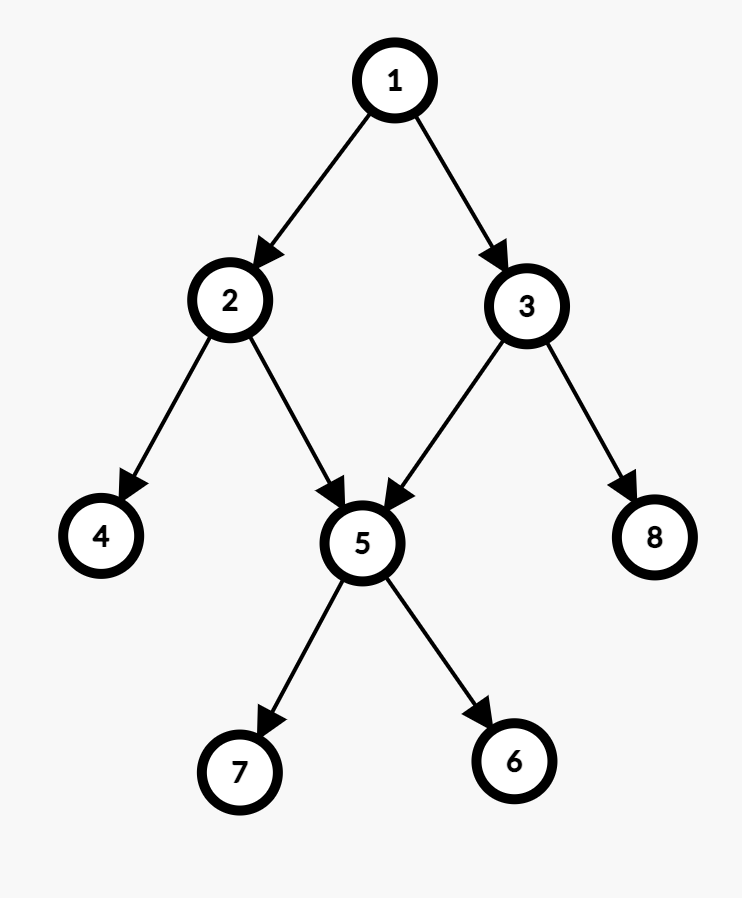
\includegraphics[width=0.43\linewidth]{20-T3/样例2.png}
        \caption{样例 2 }
        \label{fig:enter-label}
    \end{figure}

可以发现，出度为 $0$ 的点恰好就是第一类函数和第二类函数。
    
那么当遇到第三类函数时，只需要从当前点不断向下递归，直到展开成第一类函数和第二类函数，处理方式就和上一部分完全相同了。

这样做的时间复杂度为 $O(q\cdot \sum C_j)$。当某个第三类函数几乎能展开整张调用图时，同一批函数会被重复访问很多次，复杂度就会迅速失控。

不过这份暴力代码实际已经可以拿到大部分部分分。
\newpage
\begin{lstlisting}[style = code]
#include <bits/stdc++.h>
using namespace std;
typedef long long ll;
const int N = 1e5 + 10;
const int mod = 998244353;
ll a[N], b[N],c[N];
struct node {
    int op, x, y;
    vector<int> used;
} q[N];
ll mul = 1;
void dfs(int u) {
    for (auto v : q[u].used) {
        if (q[v].op == 1) {
            a[q[v].x] = (a[q[v].x] + q[v].y * mul) % mod;
        } else if (q[v].op == 2) {
            mul = mul * q[v].y % mod;
        } else {
            dfs(v);
        }
    }
};
int main() {
    int n;
    cin >> n;
    for (int i = 1; i <= n; i++) {
        cin >> a[i];
        b[i] = a[i];
        a[i] = 0;
    }
    int m;
    cin >> m;
    for (int i = 1; i <= m; i++) {
        int op, x, y;
        cin >> op;
        if (op == 1) {
            cin >> x >> y;
            q[i] = {op, x, y};
        } else if (op == 2) {
            cin >> y;
            q[i] = {op, 0, y};
        } else {
            int sz = 0;
            cin >> sz;
            vector<int> used(sz);
            for (int j = 0; j < sz; j++) {
                int x;
                cin >> x;
                used[j] = x;
            }
            reverse(used.begin(), used.end());
            q[i] = {op, 0, 0, used};
        }
    }
    int Q;
    cin >> Q;
    for (int i = 1; i <= Q; i++) {
        cin >> c[i];
    }
    for (int i = Q; i >= 1; i--) {
        int now = c[i];
        if (q[now].op == 1) {
            auto [op, x, y, used] = q[now];
            a[x] = (a[x] + y * mul) % mod;
        } else if (q[now].op == 2) {
            auto [op, x, y, used] = q[now];
            mul = mul * y % mod;
        } else {
            auto [op, x, y, used] = q[now];
            dfs(now);
        }
    }
    for (int i = 1; i <= n; i++) cout << (b[i] * mul + a[i]) % mod << " ";
    cout << '\n';
}
\end{lstlisting}

\newpage
\subsection{满分解法}

前面的暴力做法瓶颈在于第三类函数。第三类函数会继续调用一串函数，如果每次遇到它都暴力递归展开，那么同一个函数可能被重复计算很多次，复杂度会被调用关系不断放大。

由于题目保证不会出现递归调用，因此所有函数之间的调用关系构成一张有向无环图。我们只需要在这张 DAG 上做两件事：

\begin{enumerate}[leftmargin=2em,itemsep=1pt,topsep=2pt,parsep=0pt,partopsep=0pt]
    \item 先计算每个函数执行一次后，会让整个数组整体乘上多少；
    \item 再计算每个函数在最终过程中相当于被调用了多少次，并且这些调用后面还会被多少乘法放大。
\end{enumerate}

\begin{keybox}{核心思想：把函数的影响拆成 \code{mul} 和 \code{add}}
对于每个函数 $u$，维护两个量：

\begin{itemize}[leftmargin=2em,itemsep=1pt,topsep=2pt,parsep=0pt,partopsep=0pt]
    \item \code{mul[u]}：执行一次函数 $u$ 后，会让整个数组整体乘上的系数；
    \item \code{add[u]}：函数 $u$ 在最终调用过程中被执行的“有效次数”。这里的有效次数已经考虑了它后面所有乘法带来的放大。
\end{itemize}

最后真正对数组产生单点加贡献的，只有第一类函数。  
如果第一类函数 $u$ 表示 $a_p \leftarrow a_p+v$，那么它最终贡献的是
\[
v \times \mathrm{add}_u.
\]
\end{keybox}

\par\medskip
\noindent\textbf{第一步：计算每个函数的 \code{mul}}
\par\medskip

对于三类函数，\code{mul} 的定义非常直接：

\begin{itemize}[leftmargin=2em,itemsep=1pt,topsep=2pt,parsep=0pt,partopsep=0pt]
    \item 第一类函数只做单点加法，不影响整体乘法，所以 \code{mul=1}；
    \item 第二类函数会让所有数乘上 $v$，所以 \code{mul=v}；
    \item 第三类函数会依次调用若干个子函数，因此它的 \code{mul} 等于所有子函数 \code{mul} 的乘积。
\end{itemize}

也就是说，如果函数 $u$ 依次调用
\[
g_1,g_2,\ldots,g_c,
\]
那么
\[
\mathrm{mul}_u
=
\mathrm{mul}_{g_1}
\times
\mathrm{mul}_{g_2}
\times
\cdots
\times
\mathrm{mul}_{g_c}.
\]

由于调用关系是一张 DAG，可以先求出拓扑序，然后按照拓扑序的反序计算所有 \code{mul}。

\par\medskip
\noindent\textbf{第二步：倒序处理最终调用序列}
\par\medskip

设最终需要依次调用的函数为
\[
f_1,f_2,\ldots,f_Q.
\]

我们从后往前扫描这串调用序列，用变量 $M$ 维护“当前函数执行完之后，后面还会整体乘上多少”。

当扫描到函数 $f_i$ 时，函数 $f_i$ 内部产生的所有加法贡献，最后都会被当前的 $M$ 放大，因此执行：
\[
\mathrm{add}_{f_i} \mathrel{+}= M.
\]

随后，继续向前扫描时，前面的函数还会经过 $f_i$ 的整体乘法影响，所以更新：
\[
M \leftarrow M\times \mathrm{mul}_{f_i}.
\]

扫描结束后，这个 $M$ 就是整个函数序列对初始数组造成的总乘法系数。

\par\medskip
\noindent\textbf{第三步：在调用图上继续下放 \code{add}}
\par\medskip

上一步只处理了最外层调用序列。例如调用了某个第三类函数 $u$，我们只是把贡献加到了 \code{add[u]} 上，还没有分发给它内部调用的子函数。

假设函数 $u$ 依次调用
\[
g_1,g_2,\ldots,g_c.
\]

如果 \code{add[u]} 已经确定，那么每个子函数应该获得多少贡献呢？

注意：$g_i$ 执行完之后，还会继续执行它右边的函数
\[
g_{i+1},g_{i+2},\ldots,g_c.
\]
所以 $g_i$ 内部的加法贡献，还会被这些后续函数的乘法系数继续放大。

因此我们要从右往左扫描 $u$ 的子函数列表，维护一个后缀乘积 $\mathrm{suf}$：

\[
\mathrm{suf}
=
\mathrm{mul}_{g_{i+1}}
\times
\mathrm{mul}_{g_{i+2}}
\times
\cdots
\times
\mathrm{mul}_{g_c}.
\]

扫描到子函数 $g_i$ 时，执行：
\[
\mathrm{add}_{g_i}
\mathrel{+}=
\mathrm{add}_u\times \mathrm{suf}.
\]

然后更新：
\[
\mathrm{suf}
\leftarrow
\mathrm{suf}\times \mathrm{mul}_{g_i}.
\]

这个过程按照拓扑序从前往后处理即可。因为父函数一定先于它调用的子函数被处理，这样父函数的 \code{add} 才能正确下放给子函数。

\begin{keybox}{为什么要从右往左下放？}
第三类函数内部的调用是有顺序的。

对于调用序列
\[
g_1,g_2,\ldots,g_c,
\]
越靠左的函数，执行后还会经过越多后续函数的乘法影响。

因此在给子函数分配 \code{add} 时，必须从右往左维护后缀乘积。这样才能正确计算每个子函数的加法贡献会被后面的乘法放大多少。
\end{keybox}

\par\medskip
\noindent\textbf{第四步：统计第一类函数的贡献}
\par\medskip

当所有 \code{add} 都下放完成后，只需要统计第一类函数。

如果函数 $u$ 是第一类函数，表示
\[
a_p \leftarrow a_p+v,
\]
那么它最终对位置 $p$ 的贡献为
\[
v\times \mathrm{add}_u.
\]

最后，每个初始值还要乘上整段调用序列的总乘法系数。  
因此最终答案为：
\[
\text{初始值}\times \text{总乘法系数}+\text{所有第一类函数贡献}.
\]

综上，代码实现步骤如下：

\begin{enumerate}[leftmargin=2em,itemsep=1pt,topsep=2pt,parsep=0pt,partopsep=0pt]
    \item 建出函数调用 DAG，并求拓扑序；
    \item 按拓扑序反序计算每个函数的 \code{mul}；
    \item 倒序扫描最终调用序列，给对应函数累加 \code{add} 标记，同时维护总乘法系数；
    \item 按拓扑序顺序下放 \code{add}；
    \item 枚举所有第一类函数，统计单点加法贡献；
    \item 将初始数组整体乘上总乘法系数，再加上对应位置的加法贡献。
\end{enumerate}

时间复杂度为
\[
O(n+m+Q+\sum C_i).
\]

下面用一个固定的小例子，把上述几个步骤串起来演示一遍。

图中，边 $u\to v$ 表示函数 $u$ 会调用函数 $v$；叶子节点下方的 \code{*x} 表示第二类函数，\code{+v@p} 表示第一类函数，即给 $a_p$ 加上 $v$。

\begin{figure}[!htbp]
    \centering
    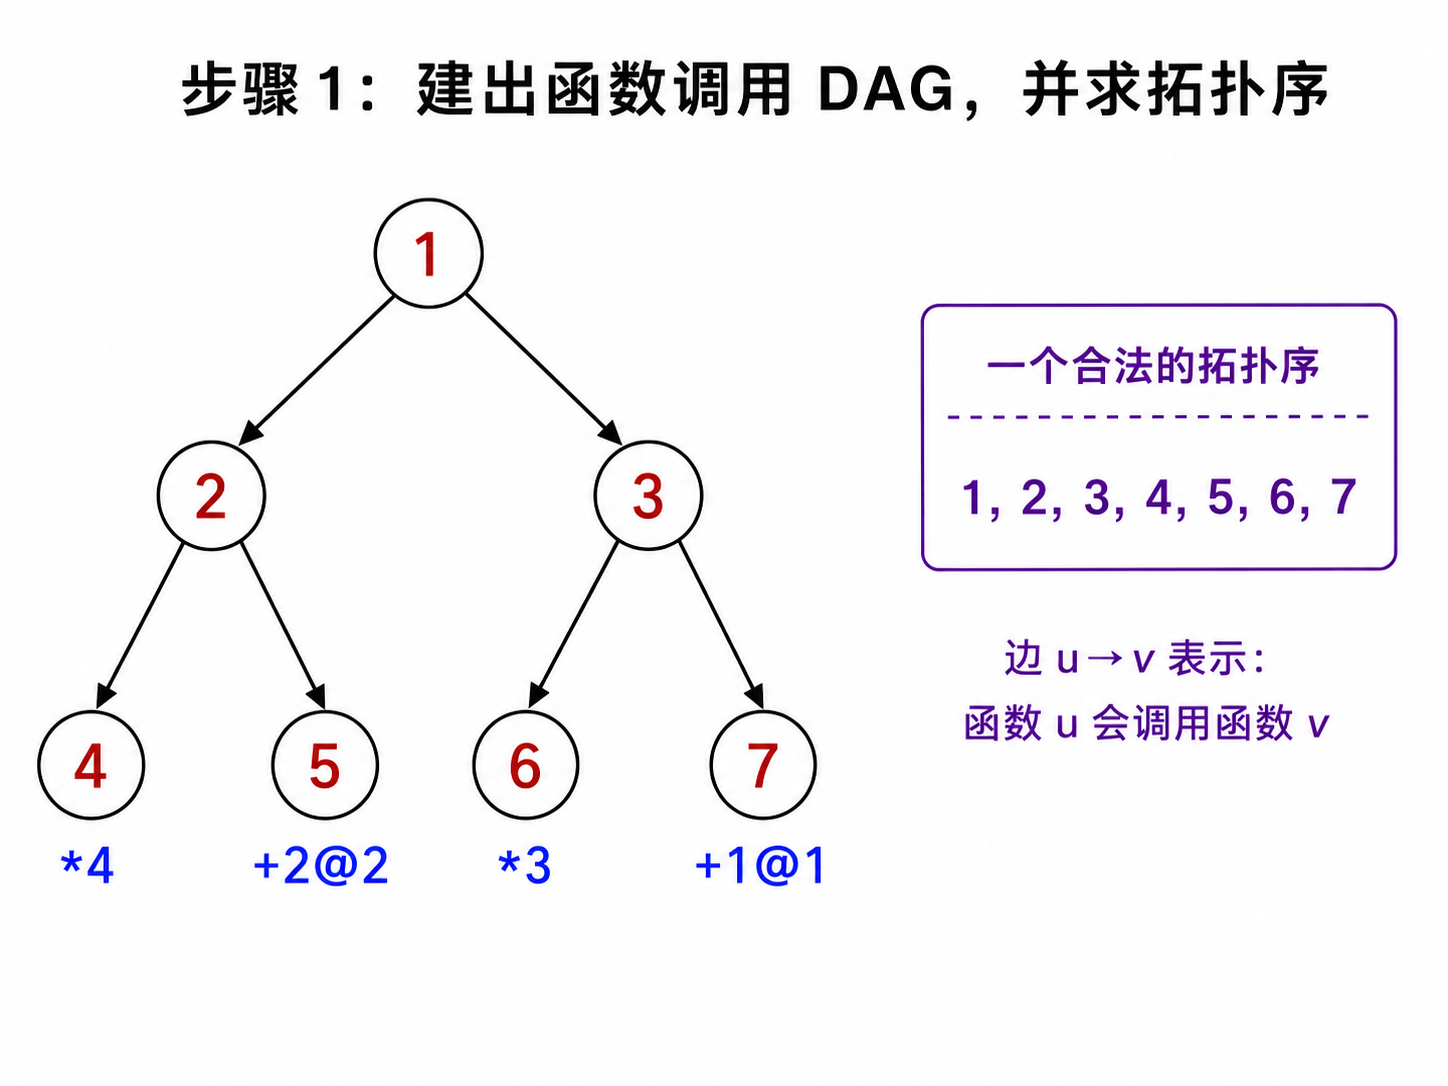
\includegraphics[width=0.49\textwidth]{20-T3/1.png}
    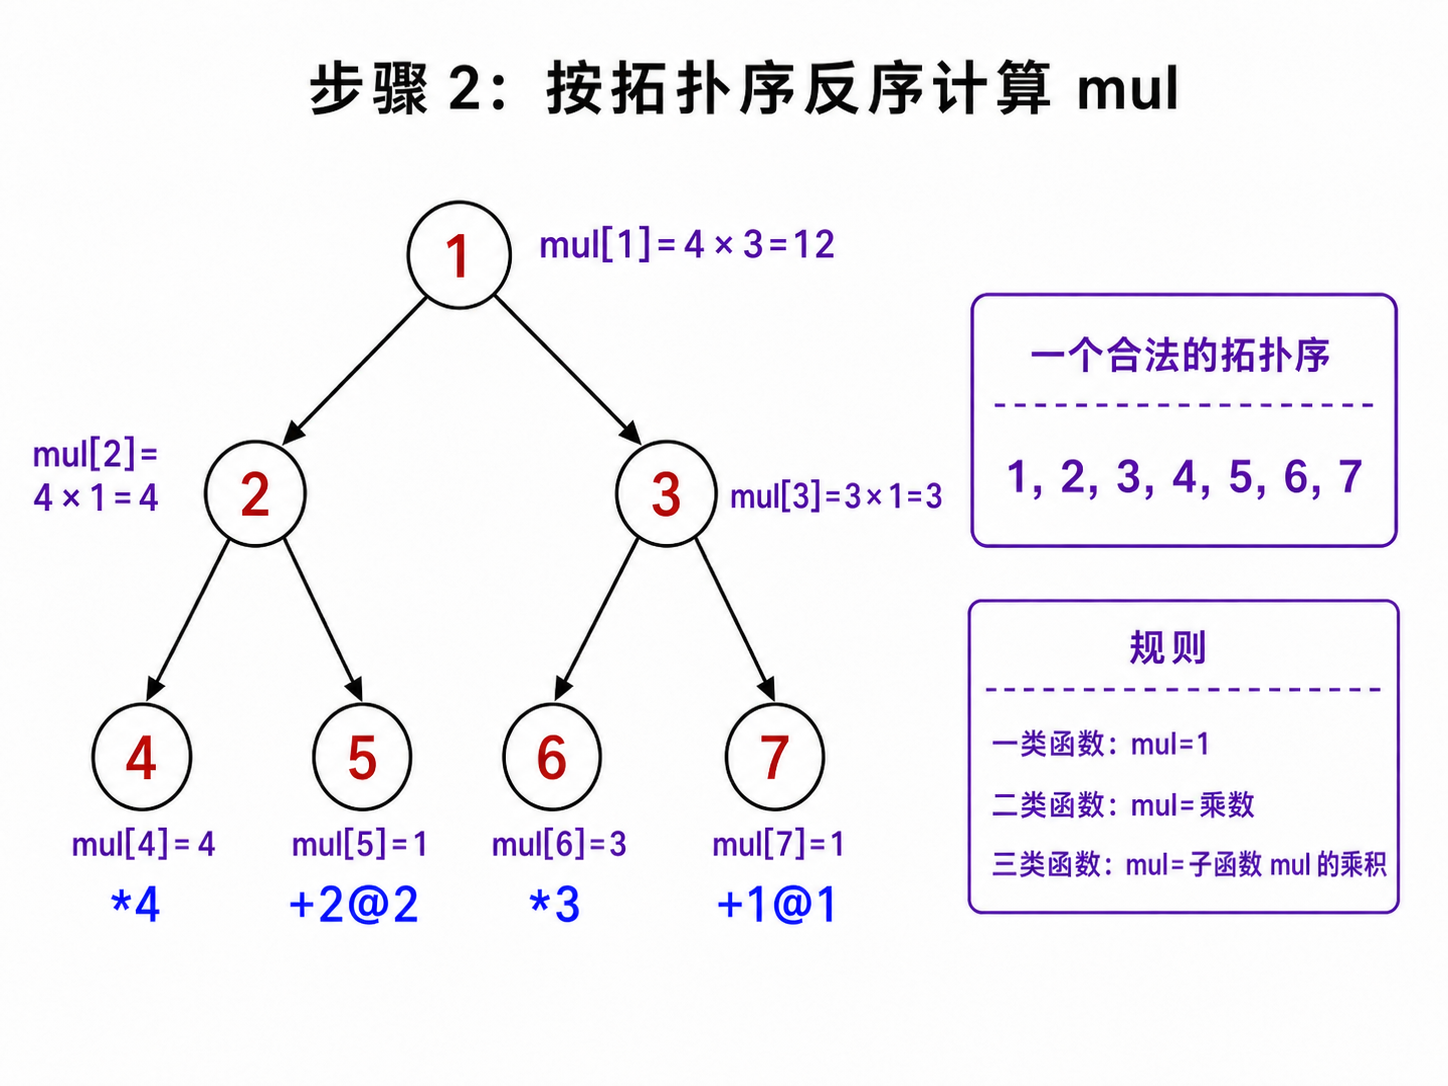
\includegraphics[width=0.49\textwidth]{20-T3/2.png}

    \vspace{0.6em}

    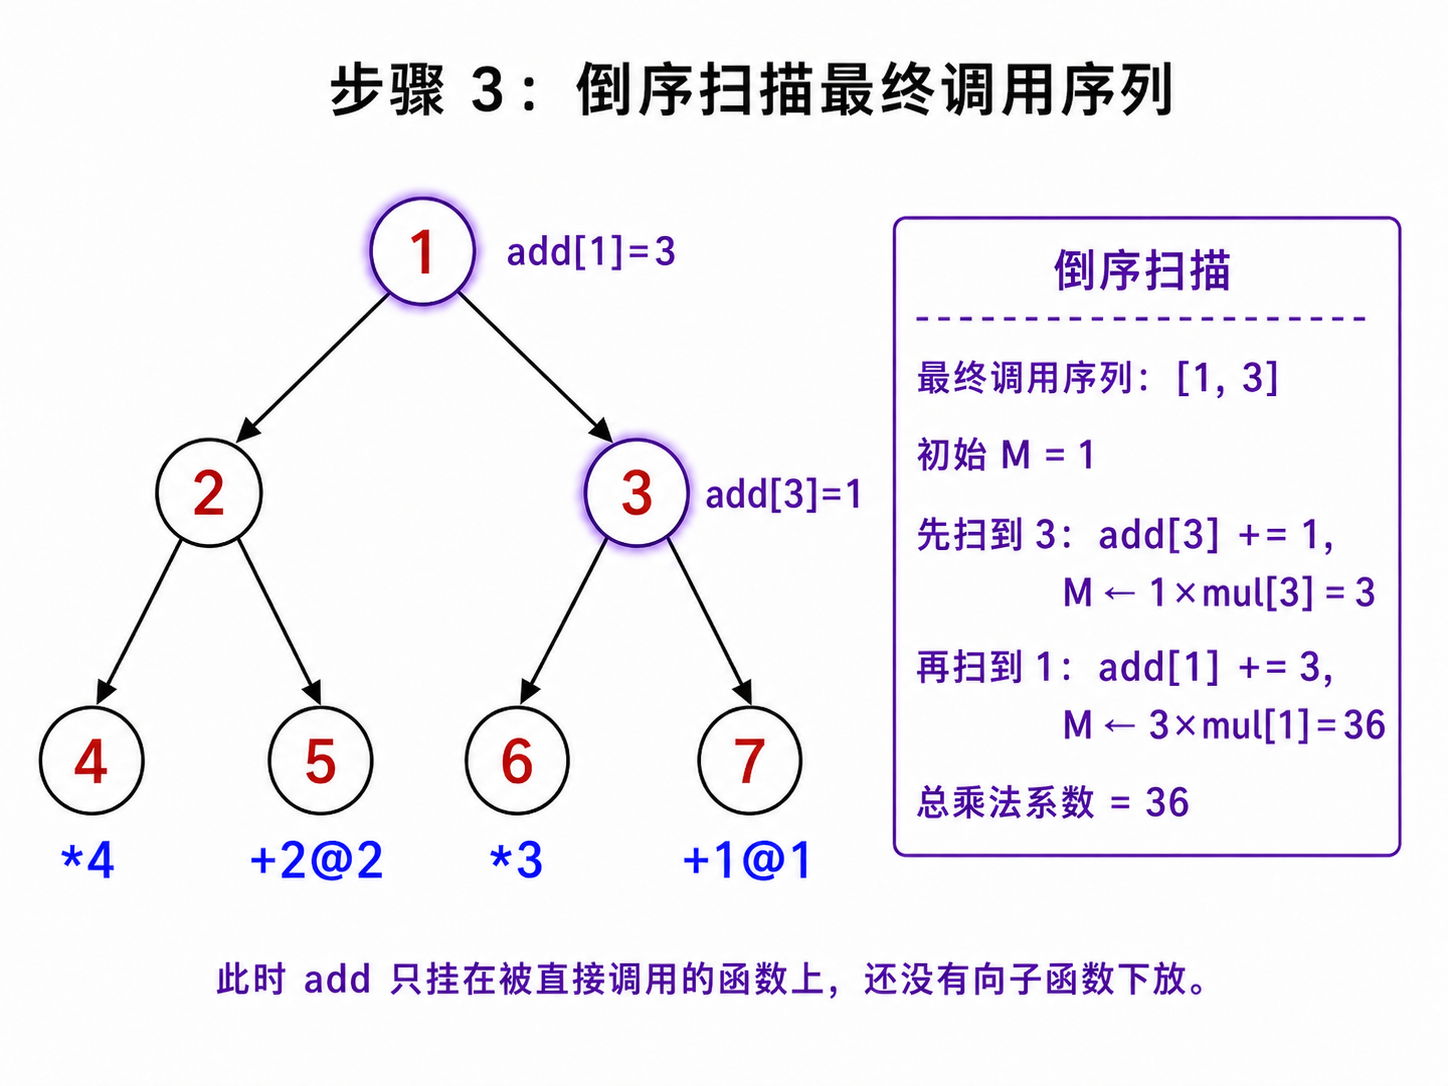
\includegraphics[width=0.7\textwidth]{20-T3/3.png}

    \vspace{0.4em}
    {\small 图中展示了建图、计算 \code{mul}、倒序扫描最终调用序列这三个步骤。}
\end{figure}

\begin{figure}[!htbp]
    \centering
    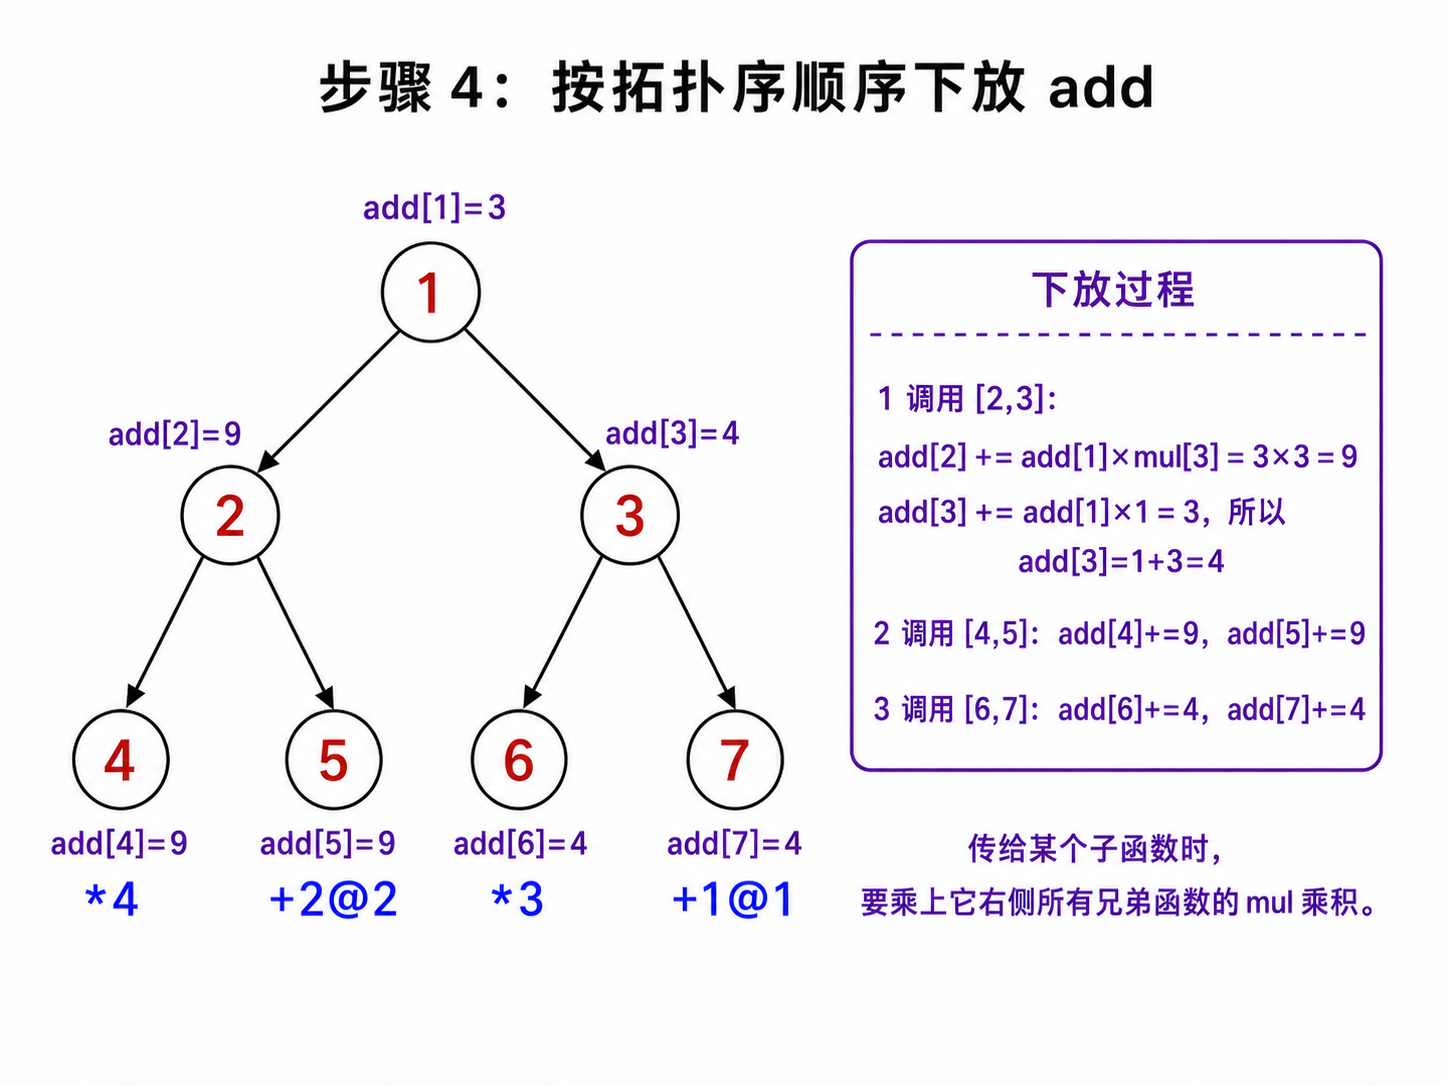
\includegraphics[width=0.7\textwidth]{20-T3/4.png}
    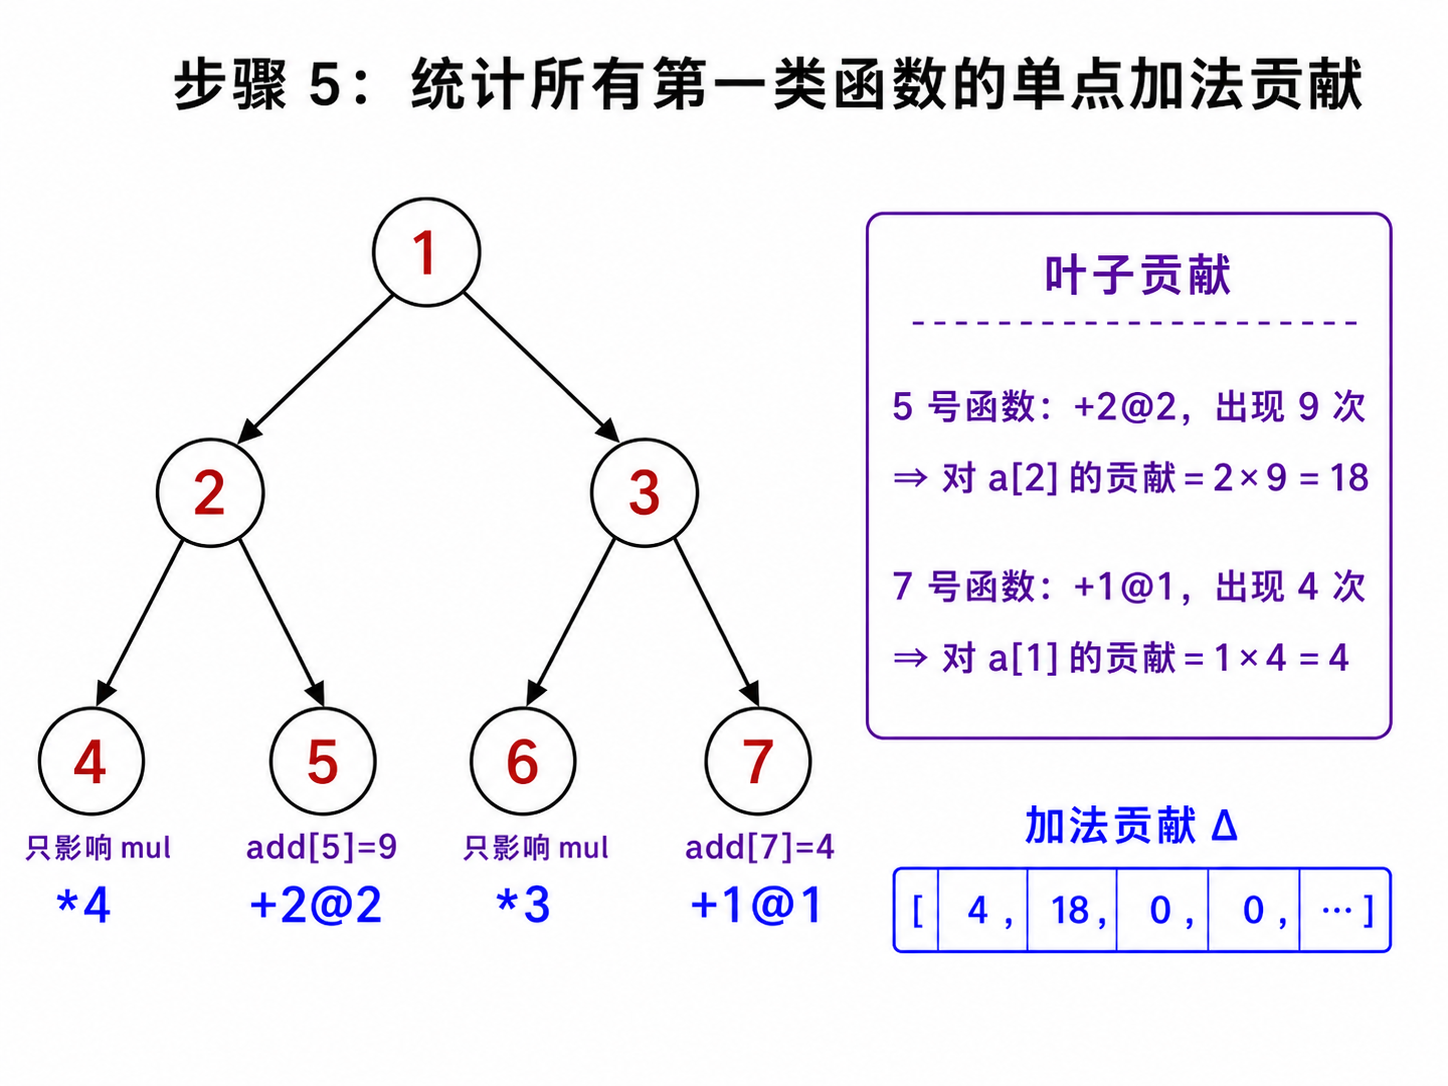
\includegraphics[width=0.7\textwidth]{20-T3/5.png}
    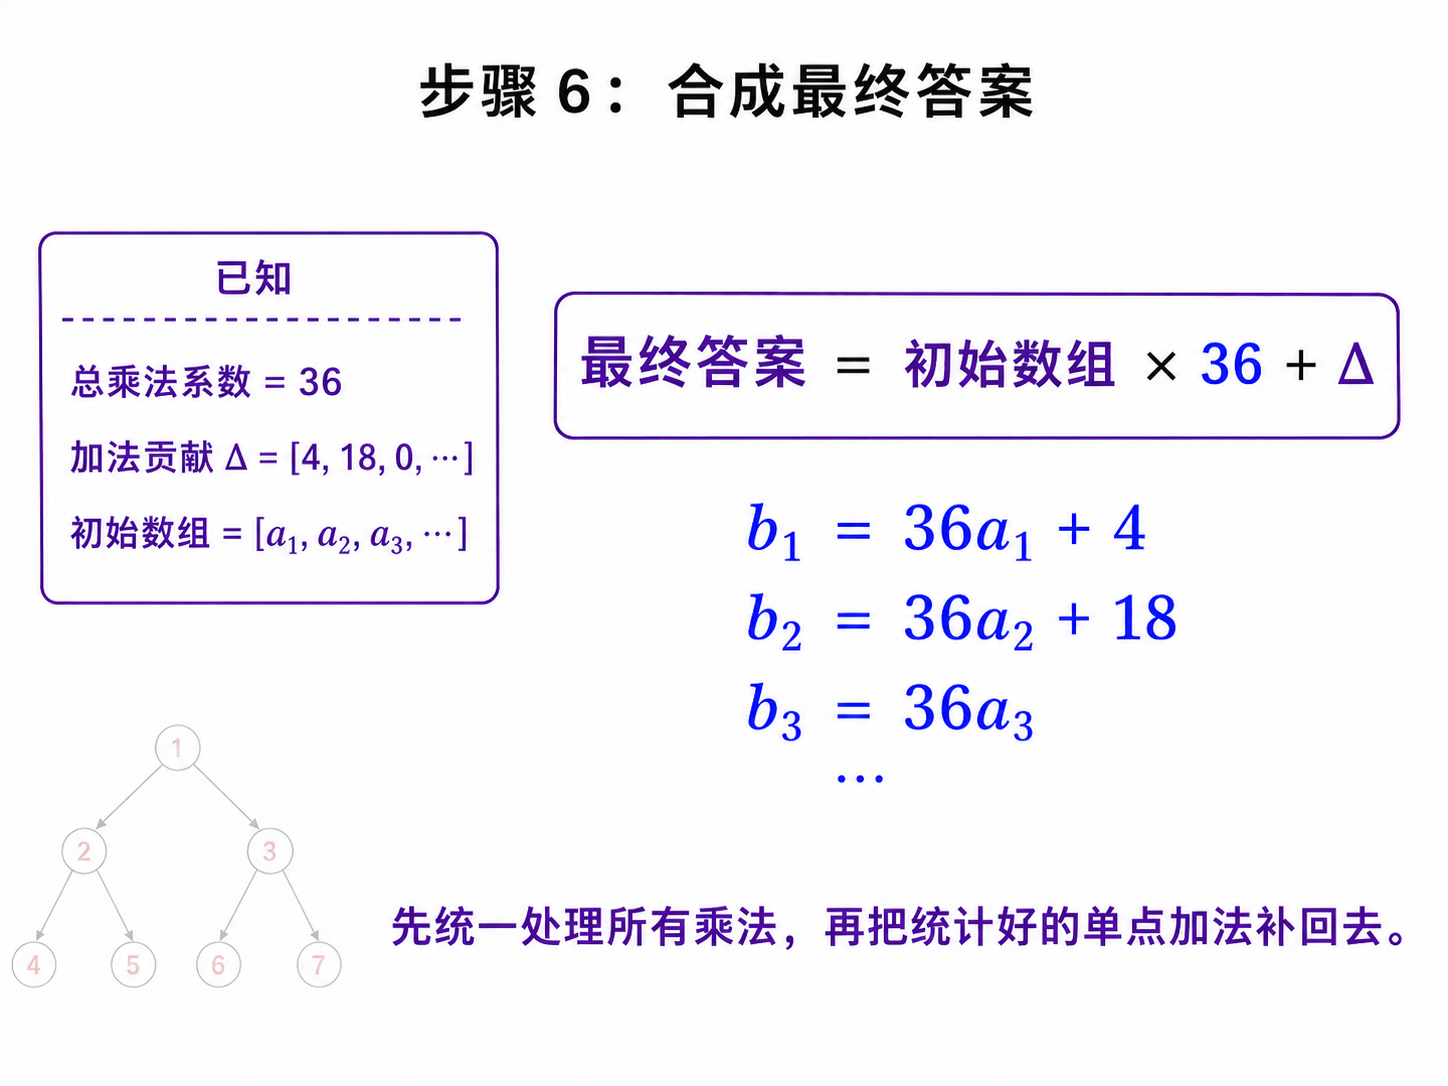
\includegraphics[width=0.7\textwidth]{20-T3/6.png}

    \vspace{0.4em}
    {\small 图中展示了下放 \code{add}、统计第一类函数贡献、合成最终答案这三个步骤。}
\end{figure}

\newpage
\begin{lstlisting}[style = code]
#include <bits/stdc++.h>
using namespace std;
typedef long long ll;
const int N = 1e5 + 10;
const int mod = 998244353;
ll a[N], b[N];
vector<int> g[N];
struct node {
    int op, p, v;
    ll add, mul;
} d[N];
int n, m, q;
int Top[N], cnt, in[N], order[N];  // Top[i]表示拓扑序为i的点的编号
void topu() {
    queue<int> q;
    for (int i = 1; i <= m; i++)if (in[i] == 0) q.push(i);
    while (!q.empty()) {
        int u = q.front();
        Top[++cnt] = u;
        q.pop();
        for (auto v : g[u]) {
            if (--in[v] == 0) q.push(v);
        }
    }
}
void getmul() {
    for (int i = cnt; i >= 1; i--) {
        int u = Top[i];
        for (auto v : g[u])d[u].mul = d[u].mul * d[v].mul % mod;
    }
}
void getadd() {
    for (int i = 1; i <= cnt; i++) {
        int u = Top[i];
        ll mul = 1;
        for (int j = g[u].size() - 1; j >= 0; j--) {
            int v = g[u][j];
            d[v].add = (d[v].add + d[u].add * mul) % mod;
            mul = mul * d[v].mul % mod;
        }
    }
}
int main() {
    cin >> n;
    for (int i = 1; i <= n; i++) cin >> a[i], b[i] = a[i], a[i] = 0;
    cin >> m;
    for (int i = 1; i <= m; i++) {
        cin >> d[i].op;
        if (d[i].op == 1)cin >> d[i].p >> d[i].v, d[i].mul = 1;
        else if (d[i].op == 2)cin >> d[i].v, d[i].mul = d[i].v;
        else {
            int sz;
            cin >> sz;
            for (int j = 0, x; j < sz; j++) {
                cin >> x;
                g[i].push_back(x),in[x]++;
            }
            d[i].mul = 1;
        }
    }
    // 步骤 1：建出函数调用 DAG 后，求拓扑序
    topu();
    // 步骤 2：反拓扑序计算每个函数的 mul
    getmul();
    cin >> q;
    for (int i = 1; i <= q; i++) cin >> order[i];
    ll mul = 1;
    // 步骤 3：倒序扫描最终调用序列
    for (int i = q; i >= 1; i--) {
        int now = order[i];
        d[now].add = (d[now].add + mul) % mod;
        mul = mul * d[now].mul % mod;
    }
    // 步骤 4：将 add 沿调用图继续下放到所有子函数
    getadd();
    // 步骤 5：枚举所有第一类函数，统计单点加法贡献
    for (int i = 1; i <= m; i++)
        if (d[i].op == 1) a[d[i].p] = (a[d[i].p] + d[i].v * d[i].add) % mod;
    // 步骤 6：初始数组整体乘上总乘法系数，再加上对应位置的加法贡献
    for (int i = 1; i <= n; i++) cout << (a[i] + b[i] * mul) % mod << ' ';
    cout << '\n';
}
\end{lstlisting}
\newpage
\section{T4. 贪吃蛇}

\subsection{题意简析}

有 $n$ 条蛇，第 $i$ 条蛇当前体力值为 $a_i$。  
两条蛇比较实力时，先比较体力值；若体力值相同，则编号更大的蛇更强。

每一轮中，当前最强的蛇拥有选择权。它可以选择：

\begin{itemize}[leftmargin=2em,itemsep=1pt,topsep=2pt,parsep=0pt,partopsep=0pt]
    \item 吃掉当前最弱的蛇，此时自己的体力值减去最弱蛇的体力值，最弱蛇退出；
    \item 选择不吃，游戏立刻结束。
\end{itemize}

每条蛇都会在\textbf{保证自己最终不被吃掉}的前提下，尽可能多吃别的蛇。  
题目要求我们求出：当所有蛇都足够聪明时，最终会剩下多少条蛇。

\subsection{从题面到模型}

这道题看起来像一道模拟题，但真正麻烦的地方并不是“每次取最强和最弱”，而是“当前最强蛇到底敢不敢吃”。

因为最强蛇一旦选择吃，自己的体力会变成
\[
x-y,
\]
其中 $x$ 是当前最强蛇体力，$y$ 是当前最弱蛇体力。这个新体力可能让它在下一轮失去优势，甚至反过来被别的蛇吃掉。

\begin{keybox}{关键观察：判断的核心不是“吃完后还是不是最强”，而是“吃完后会不会掉成最弱”}
如果一条蛇吃完后虽然不再最强，但也没有掉到最弱，那么它暂时还不处在最危险的位置；而一旦它吃完后直接变成最弱，下一轮选择权落到别人手里时，它就会立刻变得非常危险。
\end{keybox}

因此，整题的博弈判断可以统一成下面这条主线：

\begin{enumerate}[leftmargin=2em,itemsep=1pt,topsep=2pt,parsep=0pt,partopsep=0pt]
    \item 如果当前最强蛇吃完后还不是最弱，那么它一定敢吃；
    \item 如果它吃完后恰好变成最弱，那么问题就会沿着后续“最强蛇链”继续递推；
    \item 一旦进入这种递推阶段，答案最终只取决于这条链的长度奇偶性。
\end{enumerate}

前面的做法可以先用 \code{set} 把“最强”和“最弱”动态维护出来；满分做法则要进一步利用原序列本身有序的性质，把这层 `set` 去掉。

\subsection{Case 1--14：\code{set} 模拟最强最弱蛇}
\textbf{部分分特点}:$n \le 5 \times {10}^4$。

按照上面的建模，先不急着优化数据结构。只要能动态维护当前最强蛇和最弱蛇，就可以把整个判断过程直接模拟出来。

\begin{examplebox}{例子：为什么“吃完后是不是最弱”很关键？}
设当前从强到弱的几条蛇体力分别是
\[
x,\ y,\ a,\ b
\]
其中 $x$ 最强，$b$ 最弱。

若最强蛇吃掉最弱蛇，那么它的新体力变成 $x-b$。

这时会出现两种情况：

\begin{itemize}[leftmargin=2em,itemsep=1pt,topsep=2pt,parsep=0pt,partopsep=0pt]
    \item 如果 $x-b$ 吃完后仍然不是最弱蛇，那么它短时间内不会马上被吃；
    \item 如果 $x-b$ 吃完后直接变成了最弱蛇，那么下一轮选择权落到别人手里，它就很危险了。
\end{itemize}

因此，判断的关键不是“吃完后还是不是最强”，而是“\textbf{吃完后会不会掉到最弱}”。
\end{examplebox}

\begin{keybox}{关键结论 1：如果最强蛇吃完后不会变成最弱，那么它一定会吃}
原因是：此时它虽然可能失去最强地位，但还没有立刻陷入最危险的位置。

接下来轮到新的最强蛇行动。由于每条蛇都只会在保证自己不死的前提下行动，因此后面的蛇不会为了多吃一次而把前面这条蛇送去必死局面。

所以，只要当前最强蛇吃完后\textbf{还不是最弱}，它就一定敢吃。
\end{keybox}

于是，真正麻烦的只剩下一种情况：当前最强蛇吃掉最弱蛇之后，\textbf{恰好变成了当前最弱蛇}。

这时它要不要吃，就不能只看这一轮了，而要继续往后推。

设现在从强到弱依次是“老大、老二、老三、……”。  
如果老大吃完后变成最弱，那么接下来就看老二：

\begin{itemize}[leftmargin=2em,itemsep=1pt,topsep=2pt,parsep=0pt,partopsep=0pt]
    \item 如果老二吃完后不会变成最弱，那么老二一定会吃，于是老大就危险了；
    \item 如果老二吃完后也会变成最弱，那么就继续看老三；
    \item 如此递推下去，直到某一条蛇吃完后不再是最弱，或者局面只剩下两条蛇。
\end{itemize}

这说明：一旦进入这种局面，问题会沿着“最强蛇链”不断向下递归。

\begin{keybox}{关键结论 2：进入“吃完后变成最弱”的阶段后，答案只和后续链长的奇偶性有关}
如果某条蛇吃完后变成了最弱，那么下一条蛇是否会继续吃，就决定了它的生死。

继续递推下去，最终一定会遇到边界：

\begin{itemize}[leftmargin=2em,itemsep=1pt,topsep=2pt,parsep=0pt,partopsep=0pt]
    \item 要么某条蛇吃完后不再是最弱，此时它一定会吃；
    \item 要么只剩下两条蛇，此时当前最强蛇一定可以吃掉最弱蛇。
\end{itemize}

从这个边界往前倒推，就会发现：前面这些蛇“吃还是不吃”的结论是交替出现的，因此只与这段链的长度奇偶性有关。
\end{keybox}

到这里，思路就清楚了。整个过程可以分成两个阶段：

\begin{enumerate}[leftmargin=2em,itemsep=1pt,topsep=2pt,parsep=0pt,partopsep=0pt]
    \item \textbf{安全吃的阶段}：当前最强蛇吃完后还不是最弱，那么直接吃；
    \item \textbf{危险递推的阶段}：当前最强蛇吃完后变成最弱，从这里开始只需要顺着链往后判断奇偶性即可。
\end{enumerate}

如果直接用 \code{set} 维护当前所有蛇的最强和最弱，就能得到一个 $O(n\log n)$ 的做法。
\newpage
    \begin{lstlisting}[style = code]
#include <bits/stdc++.h>
using namespace std;
const int N = 1e6 + 5;
int vec[N], n;
void solve(int ca) {
    if (ca == 1) {
        cin >> n;
        for (int i = 1; i <= n; i++) cin >> vec[i];
    } else {
        int k;
        cin >> k;
        while (k--) {
            int x, y;
            cin >> x >> y;
            vec[x] = y;
        }
    }
    // first 长度 second 编号
    set<pair<int, int>> st;
    for (int i = 1; i <= n; i++) st.insert(make_pair(vec[i], i));
    int cnt = 0, ans;
    while (true) {
        // 只剩下两条蛇
        if (st.size() == 2) {
            st.erase(st.begin());  // 最强蛇可以无代价吃掉最弱
            if (cnt) {             // cnt不为零代表曾经发生过有蛇吃完变成最弱的情况
                // 根据奇偶性看一下差了多少，以此判断能否多吃一个
                if ((cnt - st.size()) & 1)
                    ans = cnt + 1;
                else
                    ans = cnt;
            } else {
                ans = 1;  // 没发生过有蛇吃完
            }
            break;
        }
        auto it = st.end();
        it--;
        auto [x, idx] = *it;
        auto [y, idy] = *st.begin();
        st.erase(it);
        st.erase(st.begin());
        st.insert(make_pair(x - y, idx));
        // 吃完之后没有变成最弱 直接吃
        if (st.begin()->second != idx) {
            // cnt不为零，代表出现过有蛇吃完变成最弱的情况
            // 这个时候最多只会吃一次，根据奇偶性进行判断
            if (cnt) {
                // 和上文同理
                if ((cnt - st.size()) & 1)
                    ans = cnt + 1;
                else
                    ans = cnt;
                break;
            }
        } else {
            // 有蛇吃完之后变成最弱了，记录一下现在剩下多少蛇
            if (cnt == 0) {
                cnt = st.size();
            }
        }
    }
    cout << ans << endl;
}
int main() {
    int t;cin >> t;
    for (int i = 1; i <= t; i++) solve(i);
}
    \end{lstlisting}

\newpage
\subsection{满分解法}

上面的思路已经把博弈本身分析清楚了，剩下要做的只是：把维护最强最弱的 \code{set} 去掉。

题目保证每组数据修改完成后，数组 $a_i$ 依然是不降的。  
因此原始的蛇天然就是有序的，我们并不需要真的把所有蛇放进平衡树里动态维护。

\begin{keybox}{关键观察：整个过程中只会新产生一类“吃完后的蛇”}
设当前最强蛇体力为 $x$，最弱蛇体力为 $y$，若它选择吃，那么会新产生一条体力为 $x-y$ 的蛇。

因此在游戏过程中，蛇可以分成两类：

\begin{itemize}[leftmargin=2em,itemsep=1pt,topsep=2pt,parsep=0pt,partopsep=0pt]
    \item 还没有参与过运算的原始蛇；
    \item 之前某一步“最强减最弱”后新产生的蛇。
\end{itemize}

前者本来就是有序的；后者也会按一定顺序加入，因此可以分别用两个双端队列维护。
\end{keybox}

具体地：

\begin{itemize}[leftmargin=2em,itemsep=1pt,topsep=2pt,parsep=0pt,partopsep=0pt]
    \item 用 \code{dq1} 存放原始蛇；
    \item 用 \code{dq2} 存放之前吃完后新产生的蛇。
\end{itemize}

此时：

\begin{itemize}[leftmargin=2em,itemsep=1pt,topsep=2pt,parsep=0pt,partopsep=0pt]
    \item 当前最弱蛇，一定在 \code{dq1} 或 \code{dq2} 的\textbf{队头}；
    \item 当前最强蛇，一定在 \code{dq1} 或 \code{dq2} 的\textbf{队尾}。
\end{itemize}

所以每一步都只需要比较两个队列的两端，就能取出当前的最强蛇和最弱蛇。

\par\medskip
\noindent\textbf{第一阶段：安全吃}

如果当前最强蛇吃掉最弱蛇后，\textbf{没有变成新的最弱蛇}，那么根据前面的结论，它一定会吃。  
于是我们把新产生的蛇加入 \code{dq2} 中，继续下一轮即可。

这里把它插入到 \code{dq2} 的队头，是因为这一阶段新产生的蛇会越来越弱，因此在 \code{dq2} 中恰好能保持顺序。

\par\medskip
\noindent\textbf{第二阶段：危险递推}

如果当前最强蛇吃掉最弱蛇后，\textbf{恰好变成了新的最弱蛇}，那么就进入前面分析过的“递推判断”阶段。

这时我们已经知道，后面的决策只取决于这条链的奇偶性。  
因此不需要再真的把这些新蛇继续塞回队列里维护，只需要继续沿着链往后模拟，直到：

\begin{itemize}[leftmargin=2em,itemsep=1pt,topsep=2pt,parsep=0pt,partopsep=0pt]
    \item 某一条蛇吃完后不再是最弱；
    \item 或者只剩下两条蛇。
\end{itemize}

然后根据这段链的长度奇偶性，就能反推出最开始那条蛇到底敢不敢吃，从而得到最终答案。由于每条蛇至多只会进出双端队列常数次，因此整体时间复杂度为 $O(n)$，空间复杂度也是 $O(n)$。

\newpage

\begin{figure}[!htbp]
    \centering
    
\includegraphics[
        width=0.98\textwidth,
        trim=0 20 0 20,
        clip
    ]{20-T4/1.png}

    \vspace{0.5em}
    {\small
    图中展示了双端队列做法：\code{dq1} 维护原始蛇，\code{dq2} 维护新产生的蛇；
    每轮从队头取最弱、从队尾取最强，并根据吃完后是否变成最弱分成两个阶段处理。
    }
\end{figure}
\newpage
    \begin{lstlisting}[style = code]
#include <bits/stdc++.h>
using namespace std;
const int N = 1e6 + 5;
using P = pair<int, int>;
int n, vec[N];

void solve(int ca) {
    // 读入本组数据：第一组完整输入，后续只做修改
    if (ca == 1) {
        cin >> n;
        for (int i = 1; i <= n; i++) cin >> vec[i];
    } else {
        int k, x, y; cin >> k;
        while (k--) { cin >> x >> y; vec[x] = y; }
    }

    // dq1：原始蛇；dq2：吃完后新产生的蛇，均维护从弱到强
    deque<P> dq1, dq2;
    for (int i = 1; i <= n; i++) dq1.push_back({vec[i], i});

    // 当前最强蛇一定在两个队列的队尾
    auto get_big = [&]() {
        P res;
        if (dq2.empty() || (!dq1.empty() && dq1.back() > dq2.back()))
             res = dq1.back(), dq1.pop_back();
        else res = dq2.back(), dq2.pop_back();
        return res;
    };

    int ans;
    while (true) {
        // 第一阶段：安全吃，直到某次吃完后变成最弱
        if (dq1.size() + dq2.size() == 2) { ans = 1; break; }
        int small = dq1.front().first; dq1.pop_front();
        auto [big, id] = get_big();
        P cur = {big - small, id};

        // cur 变成最弱，进入第二阶段
        if (dq1.empty() || dq1.front() > cur) {
            ans = dq1.size() + dq2.size() + 2;
            for (int cnt = 1; ; cnt++) {
                // 只剩两条蛇，递推到边界
                if (dq1.size() + dq2.size() + 1 == 2) {
                    if (cnt % 2 == 0) ans--;
                    break;
                }
                auto [b, i] = get_big(); cur = {b - cur.first, i};
                // cur 仍然是最弱，继续沿最强链递推
                if ((dq1.empty() || cur < dq1.front()) && (dq2.empty() || cur < dq2.front())) continue;
                // 出现吃完后不再是最弱的边界，按奇偶性反推
                if (cnt % 2 == 0) ans--;
                break;
            }
            break;
        }
        // 没变最弱，一定敢吃，新蛇放入 dq2 队头
        dq2.push_front(cur);
    }
    cout << ans << '\n';
}

int main() {
    ios::sync_with_stdio(false); 
    cin.tie(nullptr);
    int t; 
    cin >> t;
    for (int ca = 1; ca <= t; ca++) solve(ca);
    return 0;
}
\end{lstlisting}
\chapter{2021 CSP-S复赛解析}
\newpage

\section{T1. 廊桥分配}

\subsection{题意简析}

机场共有 $n$ 个廊桥，需要分配给国内区和国际区。国内航班只能使用国内区廊桥，国际航班只能使用国际区廊桥。

每架飞机按照到达时间依次处理：如果对应区域还有空闲廊桥，就停靠廊桥；否则停靠远机位。现在要求决定国内区和国际区分别分到多少个廊桥，使最终停靠廊桥的飞机数量最大。

\begin{figure}[h]
    \centering
    
\includegraphics[width=0.95\linewidth]{21-T1/1.png}
    \caption{样例 1 中不同廊桥分配方案的效果}
\end{figure}

\subsection{从题面到模型}

这道题表面上是在决定“国内区分多少个廊桥，国际区分多少个廊桥”，但两个区域之间其实只有一处耦合：它们分到的廊桥总数必须等于 $n$。一旦国内区分到 $i$ 个廊桥，国际区就只能分到 $n-i$ 个廊桥。

因此，问题可以先拆成两个彼此独立的子问题：

\begin{enumerate}[leftmargin=2em,itemsep=1pt,topsep=2pt,parsep=0pt,partopsep=0pt]
    \item 如果某个区域固定分到 $i$ 个廊桥，最多能安排多少架飞机停靠廊桥？
    \item 对所有 $0\le i\le n$，怎样组合国内区与国际区的答案，使总停靠数量最大？
\end{enumerate}

于是我们自然定义：
\[
f_1[i]=\text{国内区分到 }i\text{ 个廊桥时，最多停靠的飞机数},
\qquad
f_2[i]=\text{国际区分到 }i\text{ 个廊桥时，最多停靠的飞机数}.
\]

那么原问题就转化为
\[
\max_{0\le i\le n}\{f_1[i]+f_2[n-i]\}.
\]

\begin{keybox}{关键观察：核心在于如何高效求出单个区域的整张函数表}
最终答案的组合形式其实很直接，真正的难点是：对于同一个区域，怎样尽量快地求出 $f[0],f[1],\dots,f[n]$。

前两档部分分做法，都是“固定廊桥数后重新模拟”；满分做法则要做到“一次模拟，同时得到所有廊桥数量对应的答案”。
\end{keybox}

\newpage
\subsection{Case 1--4：直接枚举并模拟}

\textbf{部分分特点}：$n\le 100,\ m_1+m_2\le 100$。

数据范围很小，可以直接枚举国内区分到多少个廊桥。

如果国内区分到 $i$ 个廊桥，那么国际区就分到 $n-i$ 个廊桥。对于每一种分配方案，分别暴力模拟国内航班和国际航班即可。

模拟某一类航班时，先按照到达时间排序，然后维护每个廊桥当前被占用到什么时候。每架飞机到达时，顺序检查是否存在已经空闲的廊桥：如果有，就停进去；如果没有，就只能停到远机位。

这种做法复杂度为
\[
O\bigl(n^2(m_1+m_2)\bigr),
\]

\begin{lstlisting}[style = code]
typedef pair<int, int> pir;
int n, m1, m2;
pir v1[105], v2[105];
int calc(pir* v, int m, int bridge) {
    int leave[105] = {0};
    int res = 0;
    for (int i = 1; i <= m; i++) {
        for (int j = 1; j <= bridge; j++) {
            if (leave[j] < v[i].first) {
                leave[j] = v[i].second, res++;
                break;
            }
        }
    }
    return res;
}
int main() {
    cin >> n >> m1 >> m2;
    for (int i = 1; i <= m1; i++) cin >> v1[i].first >> v1[i].second;
    for (int i = 1; i <= m2; i++) cin >> v2[i].first >> v2[i].second;
    sort(v1 + 1, v1 + m1 + 1);
    sort(v2 + 1, v2 + m2 + 1);
    int ans = 0;
    for (int i = 0; i <= n; i++) {
        ans = max(ans, calc(v1, m1, i) + calc(v2, m2, n - i));
    }
    cout << ans << '\n';
    return 0;
}
\end{lstlisting}

\newpage
\subsection{Case 5--8：枚举分配方案 + 堆模拟}

\textbf{部分分特点}：$n\le 5000,\ m_1+m_2\le 5000$。

直接检查每个廊桥会比较慢，但仍然可以枚举国内区的廊桥数量。

对于某一个固定的廊桥数量，我们可以用小根堆维护当前正在使用廊桥的飞机离开时间。每架飞机到达前，先把已经离开的飞机弹出；如果当前占用数量小于分配到的廊桥数量，就让它停靠廊桥。

分别计算国内区和国际区在不同廊桥数量下能停靠的飞机数，记为 $f_1[i]$ 和 $f_2[i]$。最后枚举国内区分到 $i$ 个廊桥，答案为
\[
\max_{0\le i\le n}\{f_1[i]+f_2[n-i]\}.
\]

时间复杂度为
\[
O\bigl(n(m_1+m_2)\log(m_1+m_2)\bigr).
\]
\newpage
\begin{lstlisting}[style = code]
#include <bits/stdc++.h>
using namespace std;
const int N = 1e5 + 5;
typedef pair<int, int> pir;
int n, m1, m2;
pir v1[N], v2[N];
int f1[N], f2[N];

void get_f(pir* v, int* f, int m) {
    priority_queue<int, vector<int>, greater<int>> pq;
    for (int bridge = 1; bridge <= n; bridge++) {
        int used = 0, res = 0;
        while (!pq.empty()) pq.pop();
        for (int i = 1; i <= m; i++) {
            while (!pq.empty() && pq.top() < v[i].first) {
                pq.pop(); used--;
            }
            if (used < bridge) {
                pq.push(v[i].second);
                used++; res++;
            }
        }
        f[bridge] = res;
    }
}

int main() {
    cin >> n >> m1 >> m2;
    for (int i = 1; i <= m1; i++) cin >> v1[i].first >> v1[i].second;
    for (int i = 1; i <= m2; i++) cin >> v2[i].first >> v2[i].second;
    sort(v1 + 1, v1 + m1 + 1);
    sort(v2 + 1, v2 + m2 + 1);

    get_f(v1, f1, m1);
    get_f(v2, f2, m2);

    int ans = 0;
    for (int i = 0; i <= n; i++) ans = max(ans, f1[i] + f2[n - i]);
    
    cout << ans << '\n';
    return 0;
}
\end{lstlisting}

\subsection{满分解法}

\textbf{部分分特点}：$1\le n\le 10^5,\ m_1+m_2\le 10^5$。

前面的做法慢在：每枚举一种廊桥分配，都要重新模拟一遍。换句话说，我们虽然已经知道答案一定具有
\[
\max_{0\le i\le n}\{f_1[i]+f_2[n-i]\}
\]
这样的形式，却还没有高效求出这两张函数表。

下面考虑怎样对单个区域只做一次模拟，就同时得到所有 $f[i]$。

\begin{keybox}{关键观察：一次模拟求出所有廊桥数量的答案}
对于某一个区域，我们假设廊桥数量足够多，并且每架飞机到达时，都停靠到编号最小的空闲廊桥。

如果某架飞机在这次模拟中被分配到了编号为 $id$ 的廊桥，那么当这个区域只有 $x$ 个廊桥时，它能停靠廊桥，当且仅当 $x\ge id$。

因此，只需要统计每个廊桥编号被使用了多少次，再做前缀和，就能得到这个区域分配 $0,1,2,\ldots,n$ 个廊桥时分别能停靠多少架飞机。
\end{keybox}

为什么这个结论成立呢？

如果一架飞机在“优先使用最小编号空闲廊桥”的模拟中使用了第 $id$ 个廊桥，说明它到达时，编号 $1\sim id-1$ 的廊桥都正在被占用。

所以如果这个区域只有 $x<id$ 个廊桥，它一定停不进去；如果有 $x\ge id$ 个廊桥，它仍然可以停靠在第 $id$ 个廊桥。

于是，我们只需要对每个区域做一次模拟。

具体做法如下：

\begin{enumerate}[leftmargin=2em,itemsep=1pt,topsep=2pt,parsep=0pt,partopsep=0pt]
    \item 将该区域的所有航班按照到达时间排序；
    \item 用一个小根堆维护空闲廊桥编号；
    \item 用另一个小根堆维护正在使用的廊桥，元素为“离开时间、廊桥编号”；
    \item 每架飞机到达前，先释放所有已经离开的廊桥；
    \item 如果还有空闲廊桥，就取编号最小的廊桥给它，并令该编号的使用次数加一；
    \item 最后对每个编号的使用次数做前缀和。
\end{enumerate}

设国内区预处理得到 $f_1[i]$，国际区预处理得到 $f_2[i]$。最终答案为
\[
\max_{0\le i\le n}\{f_1[i]+f_2[n-i]\}.
\]

时间复杂度为
\[
O\bigl((n+m_1+m_2)\log n\bigr).
\]
\newpage

\begin{lstlisting}[style = code]
#include <bits/stdc++.h>
using namespace std;
const int N = 1e5 + 5;
typedef pair<int, int> pir;
int n, m1, m2, f1[N], f2[N], cnt[N];
pir v1[N], v2[N];

void get_f(pir* v, int* f, int m) {
    sort(v + 1, v + m + 1);
    priority_queue<int, vector<int>, greater<int>> free_id;
    priority_queue<pir, vector<pir>, greater<pir>> busy;
    for (int i = 1; i <= n; i++) {
        free_id.push(i);
        cnt[i] = f[i] = 0;
    }
    f[0] = 0;

    for (int i = 1; i <= m; i++) {
        int arr = v[i].first, lea = v[i].second;
        while (!busy.empty() && busy.top().first < arr) {
            free_id.push(busy.top().second);
            busy.pop();
        }
        if (free_id.empty()) continue;
        int id = free_id.top(); free_id.pop();
        cnt[id]++; busy.push({lea, id});
    }
    for (int i = 1; i <= n; i++) f[i] = f[i - 1] + cnt[i];
}

int main() {
    ios::sync_with_stdio(false); cin.tie(nullptr);
    cin >> n >> m1 >> m2;
    for (int i = 1; i <= m1; i++) cin >> v1[i].first >> v1[i].second;
    for (int i = 1; i <= m2; i++) cin >> v2[i].first >> v2[i].second;

    get_f(v1, f1, m1); get_f(v2, f2, m2);
    int ans = 0;
    for (int i = 0; i <= n; i++) ans = max(ans, f1[i] + f2[n - i]);
    cout << ans << '\n';
    return 0;
}
\end{lstlisting}
\newpage
\section{T2. 括号序列}

\subsection{题意简析}

给定一个长度为 $n$ 的字符串，字符可能是 \code{(}、\code{)}、\code{*} 或 \code{?}。其中 \code{?} 可以被替换成前三种字符中的任意一种。

我们需要统计有多少种替换方式，使得最终字符串成为一个符合定义的“超级括号序列”。答案对 $10^9+7$ 取模。

和普通括号序列相比，本题多了字符 \code{*}。它可以出现在括号结构内部，也可以夹在两个合法结构之间，但连续的一段 \code{*} 长度不能超过 $k$，并且不能作为整个序列裸露在最外层。

\begin{examplebox}{规范超级括号序列示例解释}
以 $k=3$ 为例，\code{((**()*(*))*)(***)} 是合法的。

它可以看成两个合法部分拼接而成：
\[
\code{((**()*(*))*)}\quad \code{(***)}.
\]

其中，第二部分 \code{(***)} 是形如 \code{(S)} 的结构，里面的 \code{S=***}，长度为 $3$，没有超过 $k$。

第一部分可以看成形如 \code{(AS)} 的结构：外层括号内部先放一个合法结构，再接上一段长度为 $1$ 的 \code{*}。

下面几个例子不合法：

\begin{itemize}[leftmargin=2em,itemsep=1pt,topsep=2pt,parsep=0pt,partopsep=0pt]
    \item \code{*()}：不能以裸露的 \code{*} 开头；
    \item \code{(*()*)}：中间的 \code{*()*} 无法作为合法结构出现；
    \item \code{((**))*)}：括号不匹配；
    \item \code{(****(*))}：连续 \code{*} 的长度超过了 $k=3$。
\end{itemize}
\end{examplebox}

\subsection{从题面到模型}

这道题的难点不在于把 \code{?} 替换成什么字符，而在于“合法超级括号序列”本身带有递归结构。把题意整理后，可以把一个合法串看成由下面几类基本结构递归生成：

\begin{enumerate}[leftmargin=2em,itemsep=1pt,topsep=2pt,parsep=0pt,partopsep=0pt]
    \item 一个被最外层括号包住的整体：\code{()}、\code{(S)}、\code{(A)}、\code{(AS)}、\code{(SA)}；
    \item 两个合法结构的拼接：\code{AB}；
    \item 中间夹着一段星号的拼接：\code{ASB}。
\end{enumerate}

这里 $S$ 表示长度不超过 $k$ 的纯 \code{*} 串，$A,B$ 表示合法超级括号序列。

如果只是判断某个区间能否合法，用一个布尔状态就够了；但本题要求统计方案数，直接设
\[
g[l][r]=[l,r]\text{ 成为合法超级括号序列的方案数}
\]
会在拼接时产生重复计数。

例如 \code{()()()} 既可以拆成
\[
\code{()}+\code{()()}
\]
也可以拆成
\[
\code{()()}+\code{()}
\]
这两种拆法对应的是同一个最终字符串，却会在转移中被重复统计。

\begin{keybox}{关键观察：拼接时必须固定拆分标准}
要避免重复计数，就不能让同一个合法串被不同分割点反复表示。一个自然的办法是规定：在拼接转移中，最右边那一段必须是一个“被最外层括号包住的整体”。
\end{keybox}

于是把状态拆成两类：
\[
dp[l][r]=[l,r]\text{ 是一个被最外层括号包住的合法整体的方案数},
\]
\[
f[l][r]=[l,r]\text{ 是一个拼接型合法序列的方案数}.
\]

这样一来，任意合法区间 $[l,r]$ 的总方案数就是
\[
dp[l][r]+f[l][r].
\]

前面的最小数据可以先暴力枚举所有填法，再用布尔区间 DP 判断是否合法；而从正解角度看，真正需要建立的就是上面这一组区间计数状态。
\subsection{Case 1--3：DFS 枚举所有填法}

\textbf{部分分特点}：$n\le 15$。

这一部分数据范围很小，可以直接枚举每一个 \code{?} 的取值。每个 \code{?} 可以填成 \code{(}、\code{)}、\code{*} 三种字符，因此最多有 $3^n$ 种填法。

对于每一种填好的字符串，我们再判断它是否是一个合法的超级括号序列。

这里不建议手写复杂的字符串递归拆分，而是使用一个布尔版区间 DP 来判断。因为在判断阶段，我们只关心“这个区间是否合法”，不需要统计方案数，也不需要考虑重复计数问题。

\par\medskip
\noindent\textbf{布尔 DP 状态}
\par\medskip

设当前已经填好的字符串为 \code{s}。

我们维护四类状态：

\begin{itemize}[leftmargin=2em,itemsep=1pt,topsep=2pt,parsep=0pt,partopsep=0pt]
    \item \code{S[l][r]}：区间 $[l,r]$ 是否是一段长度不超过 $k$ 的纯 \code{*} 串；
    \item \code{A[l][r]}：区间 $[l,r]$ 是否是一个合法的超级括号序列；
    \item \code{AS[l][r]}：区间 $[l,r]$ 是否可以表示成“合法序列 $+$ 星号段”；
    \item \code{SA[l][r]}：区间 $[l,r]$ 是否可以表示成“星号段 $+$ 合法序列”。
\end{itemize}

其中 \code{AS} 和 \code{SA} 是辅助状态，用来处理规则中的 \code{(AS)}、\code{(SA)} 以及 \code{ASB} 结构。

\par\medskip
\noindent\textbf{转移方式}
\par\medskip

首先预处理所有合法的 \code{S[l][r]}，也就是判断区间 $[l,r]$ 是否全为 \code{*}，并且长度不超过 $k$。

然后按区间长度从小到大转移：

\begin{enumerate}[leftmargin=2em,itemsep=1pt,topsep=2pt,parsep=0pt,partopsep=0pt]
    \item 如果 $s_l=\code{(}$ 且 $s_r=\code{)}$，则可以尝试形成 \code{()}、\code{(S)}、\code{(A)}、\code{(AS)}、\code{(SA)}；
    \item 枚举分割点，尝试把区间拆成 \code{AB}；
    \item 枚举分割点，尝试把区间拆成 \code{ASB}；
    \item 顺手维护 \code{AS} 和 \code{SA}，供更长的区间使用。
\end{enumerate}

如果最终 \code{A[1][n]} 为真，说明当前填法是合法的。

复杂度方面，设 \code{?} 的个数为 $q$，DFS 枚举最多有 $3^q$ 种填法。每次判断合法性时，布尔区间 DP 的复杂度为 $O(n^3)$，因此总时间复杂度为 $O(3^n\cdot n^3)$。
\newpage
\begin{lstlisting}[style = code]
#include <bits/stdc++.h>
using namespace std;
int n, k, ans; 
string original_s, s;
bool A[N][N], S[N][N], AS[N][N], SA[N][N];
bool check() {
    memset(A, 0, sizeof(A));
    memset(S, 0, sizeof(S));
    memset(AS, 0, sizeof(AS));
    memset(SA, 0, sizeof(SA));
    for (int l = 1; l <= n; l++) {
        for (int r = l; r <= n && r - l + 1 <= k; r++) {
            bool ok = true;
            for (int p = l; p <= r; p++) if (s[p] != '*') ok = false;
            S[l][r] = ok;
        }
    }
    for (int len = 2; len <= n; len++) {
        for (int l = 1, r = len; r <= n; l++, r++) {
            // 最外层是 (...) 的情况
            if (s[l] == '(' && s[r] == ')') {
                if (len == 2)                 A[l][r] = true; 
                else if (S[l + 1][r - 1])     A[l][r] = true; 
                else if (A[l + 1][r - 1])     A[l][r] = true; 
                else if (AS[l + 1][r - 1])    A[l][r] = true; 
                else if (SA[l + 1][r - 1])    A[l][r] = true; 
            }
            // AB 或 ASB
            for (int mid = l; mid < r; mid++) {
                if (A[l][mid] && A[mid + 1][r]) A[l][r] = true;
                if (AS[l][mid] && A[mid + 1][r]) A[l][r] = true;
            }
            // 维护 AS 和 SA
            for (int mid = l; mid < r; mid++) {
                if (A[l][mid] && S[mid + 1][r]) AS[l][r] = true;
                if (S[l][mid] && A[mid + 1][r]) SA[l][r] = true;
            }
        }
    }
    return A[1][n];
}

bool pre_check() {
    int bal = 0, star = 0; // bal 替代原有的左右括号计数
    for (int i = 1; i <= n; i++) {
        if (s[i] == '(') bal++, star = 0;
        else if (s[i] == ')') bal--, star = 0;
        else star++;
        if (bal < 0 || star > k) return false;
    }
    return bal == 0;
}
void dfs(int pos) {
    if (pos > n) { if (pre_check() && check()) ans++; return; }
    for (char c : {'(', ')', '*'}) {
        if (original_s[pos] == '?' || original_s[pos] == c) {
            s[pos] = c; 
            dfs(pos + 1);
        }
    }
}
int main() {
    string tmp; 
    cin >> n >> k >> tmp;
    original_s = s = " " + tmp; 
    dfs(1);
    cout << ans << '\n';
}
\end{lstlisting}
\subsection{Case 4--13：区间 DP}

\textbf{部分分特点}：$n\le 100$。

既然已经把合法结构拆成了 $dp$ 和 $f$ 两类状态，这一部分就可以直接按照这套建模做区间 DP。

由于原串中含有 \code{?}，判断某个位置能否作为左括号、右括号或星号时，需要写成：

\begin{itemize}[leftmargin=2em,itemsep=1pt,topsep=2pt,parsep=0pt,partopsep=0pt]
    \item 可以作为左括号：原字符是 \code{(} 或 \code{?}；
    \item 可以作为右括号：原字符是 \code{)} 或 \code{?}；
    \item 可以作为星号：原字符是 \code{*} 或 \code{?}。
\end{itemize}
\newpage
\par\medskip
\noindent\textbf{转移一：最外层括号整体}
\par\medskip

如果第 $l$ 位可以填成 \code{(}，第 $r$ 位可以填成 \code{)}，那么可以尝试让它们作为最外层匹配括号。

首先，内部可以直接是一个合法序列，也可以为空：

$$
dp[l][r]\mathrel{+}=dp[l+1][r-1]+f[l+1][r-1]
$$

这里把空区间视为一种合法的内部结构，用来处理 \code{()}。

接下来考虑右侧带一段星号，也就是 \code{(AS)} 或 \code{(S)}。设区间 $[t,r-1]$ 是一段长度不超过 $k$ 的纯星号段，则有：

$$
dp[l][r]\mathrel{+}=dp[l+1][t-1]+f[l+1][t-1]
$$

其中当 $[l+1,t-1]$ 为空时，对应的就是 \code{(S)}。

类似地，考虑左侧带一段星号，也就是 \code{(SA)}。设区间 $[l+1,t]$ 是一段长度不超过 $k$ 的纯星号段，则有：

$$
dp[l][r]\mathrel{+}=dp[t+1][r-1]+f[t+1][r-1]
$$

\par\medskip
\noindent\textbf{转移二：拼接型合法序列}
\par\medskip

拼接型合法序列有两种来源，它们正对应题面中的两类拼接方式。

第一种是 \code{AB}。左侧可以是任意合法序列，右侧必须固定为一个被最外层括号包住的整体：

$$
f[l][r]\mathrel{+}=
\sum_{mid=l}^{r-1}
\bigl(dp[l][mid]+f[l][mid]\bigr)\times dp[mid+1][r]
$$

第二种是 \code{ASB}。设中间的星号段为 $[st,ed]$，它必须是一段长度不超过 $k$ 的纯星号段。左侧可以是任意合法序列，右侧仍然固定为一个 $dp$ 整体：

$$
f[l][r]\mathrel{+}=
\sum
\bigl(dp[l][st-1]+f[l][st-1]\bigr)\times dp[ed+1][r]
$$

其中求和范围为：

$$
l<st\le ed<r,\qquad [st,ed]\text{ 是一段合法的 }S
$$

这里右侧只使用 $dp[ed+1][r]$，本质上就是在固定“最后一个整体”的位置，从而避免前面提到的重复计数。

朴素实现中，\code{ASB} 需要枚举星号段的左右端点，因此总时间复杂度为：

$$
O(n^4)
$$

\newpage
\begin{lstlisting}[style = code]
#include <bits/stdc++.h>
using namespace std;
typedef long long ll;
const int mod = 1e9 + 7;
const int N = 105;

ll dp[N][N];     // 被最外层括号包住的合法整体
ll f[N][N];      // 拼接型合法序列
bool is_S[N][N]; // 预处理 [l, r] 是否为纯星号段 S
int n, k; 
string s;
bool can_L(int i) { return s[i] == '(' || s[i] == '?'; }
bool can_R(int i) { return s[i] == ')' || s[i] == '?'; }
bool can_star(int i) { return s[i] == '*' || s[i] == '?'; }
void add(ll &x, ll y) { x = (x + y) % mod; }

int main() {
    cin >> n >> k >> s;
    s = " " + s;
    // 预处理 is_S[l][r]
    for (int l = 1; l <= n; l++) {
        for (int r = l; r <= min(n, l + k - 1); r++) {
            bool ok = true;
            for (int p = l; p <= r; p++) {
                if (!can_star(p)) { 
                    ok = false; 
                    break; 
                }
            }
            is_S[l][r] = ok;
        }
    }
    for (int len = 2; len <= n; len++) {
        for (int l = 1, r = len; r <= n; l++, r++) {
            // ===== 转移一：最外层括号整体 (dp) =====
            if (can_L(l) && can_R(r)) {
                if (len == 2) {
                    add(dp[l][r], 1); 
                } else {
                    // 1. 内部是合法序列 (A)，或者为空 ()
                    add(dp[l][r], dp[l + 1][r - 1] + f[l + 1][r - 1]);
                    // 2. 内部是 (S)
                    if (is_S[l + 1][r - 1]) add(dp[l][r], 1);
                    // 3. (AS) -> A: [l+1, t-1], S: [t, r-1]
                    for (int t = l + 2; t <= r - 1; t++) {
                        if (is_S[t][r - 1]) {
                            add(dp[l][r], dp[l + 1][t - 1] + 
                                          f[l + 1][t - 1]);
                        }
                    }
                    
                    // 4. (SA) -> S: [l+1, t], A: [t+1, r-1]
                    for (int t = l + 1; t <= r - 2; t++) {
                        if (is_S[l + 1][t]) {
                            add(dp[l][r], dp[t + 1][r - 1] + 
                                          f[t + 1][r - 1]);
                        }
                    }
                }
            }

            // ===== 转移二：拼接型合法序列 (f) =====
            // 1. AB 
            // A 为任意合法序列，B 固定为被外层包住的整体
            for (int mid = l; mid < r; mid++) {
                ll l_val = (dp[l][mid] + f[l][mid]) % mod;
                add(f[l][r], l_val * dp[mid + 1][r]);
            }
            // 2. ASB 
            // A 为任意合法序列，S 为 [st, ed]，B 固定为整体
            for (int st = l + 1; st < r; st++) {
                for (int ed = st; ed < r; ed++) {
                    if (is_S[st][ed]) {
                        ll l_val = (dp[l][st - 1] + f[l][st - 1]) % mod;
                        add(f[l][r], l_val * dp[ed + 1][r]);
                    }
                }
            }
        }
    }
    cout << (dp[1][n] + f[1][n]) % mod << '\n';
}
\end{lstlisting}

\newpage
\subsection{满分解法：优化 \code{ASB} 转移}

\textbf{部分分特点}：$n\le 500$。

上一部分的区间 DP 已经找到了正确的状态设计，接下来只需要继续优化实现。真正拖慢复杂度的是 \code{ASB} 的转移。

在固定区间 $[l,r]$ 时，我们需要枚举中间星号段 $[st,ed]$，转移形式为：

$$
f[l][r]\mathrel{+}=
\bigl(dp[l][st-1]+f[l][st-1]\bigr)\times dp[ed+1][r]
$$

其中 $[st,ed]$ 必须是一段长度不超过 $k$ 的纯星号段。

朴素写法会同时枚举 $st$ 和 $ed$，因此这一部分对每个区间都是 $O(n^2)$ 的，整体复杂度达到 $O(n^4)$。

\begin{keybox}{关键观察：固定星号段右端点，维护所有左端点贡献}
对于固定的 $l,r$，从左到右枚举星号段右端点 $ed$。

当 $ed$ 固定时，所有合法的左端点 $st$ 一定构成一段连续区间，并且这段星号区间长度不能超过 $k$。

因此，我们可以用双指针维护当前所有合法左端点的贡献和。设

$$
\mathrm{sum}
=
\sum
\bigl(dp[l][st-1]+f[l][st-1]\bigr)
$$

其中 $st$ 枚举当前所有合法的星号段左端点。

那么对于当前的 $ed$，所有 \code{ASB} 的贡献可以一次性加入：

$$
f[l][r]\mathrel{+}=
\mathrm{sum}\times dp[ed+1][r]
$$
\end{keybox}

具体维护时，我们从左到右枚举 $ed$：

\begin{enumerate}[leftmargin=2em,itemsep=1pt,topsep=2pt,parsep=0pt,partopsep=0pt]
    \item 如果第 $ed$ 位可以作为 \code{*}，就把新的左端点 $st=ed$ 对应的贡献加入 \code{sum}；
    \item 如果当前星号段长度超过 $k$，就不断右移左端点，并从 \code{sum} 中删去过期贡献；
    \item 如果第 $ed$ 位不能作为 \code{*}，说明连续星号段断开，直接清空 \code{sum}，并从下一个位置重新开始。
\end{enumerate}

这样，每个区间 $[l,r]$ 的 \code{ASB} 转移就从 $O(n^2)$ 优化到了 $O(n)$。其余转移仍然与 Case 4--13 完全相同，因此总时间复杂度变为：

$$
O(n^3)
$$

\newpage
下面只展示需要替换的 \code{ASB} 转移部分，其余代码与上一部分相同。

\begin{lstlisting}[style = code]
void del(ll &x, ll y) {
    x = (x - y + mod) % mod;
}
// 原来的 ASB 转移需要枚举 st 和 ed
// 这里改为固定 ed，用双指针维护所有合法 st 的贡献和
ll sum = 0;

for (int ed = l + 1, st = l + 1; ed < r; ed++) {
    if (can_star(ed)) {
        // 新增左端点 st = ed 的贡献
        add(sum, dp[l][ed - 1] + f[l][ed - 1]);

        // 星号段长度不能超过 k，删去过期左端点
        while (ed - st + 1 > k) {
            del(sum, dp[l][st - 1] + f[l][st - 1]);
            st++;
        }
    } else {
        // 连续星号段断开，重新开始维护
        st = ed + 1;
        sum = 0;
    }

    // 当前所有合法 [st, ed] 的贡献一次性加入
    add(f[l][r], sum * dp[ed + 1][r] % mod);
}
\end{lstlisting}
\newpage
\section{T3. 回文}

\subsection{题意简析}

给定一个长度为 $2n$ 的序列 $a$，其中 $1\sim n$ 每个数都恰好出现两次。每次可以从当前序列的左端或右端取出一个数，接到新序列 $b$ 的末尾。要求判断能否让 $b$ 成为回文序列；若可以，需要输出字典序最小的操作串。

\subsection{从题面到模型}

这道题的表面操作只有一件事：每一步从当前序列两端取一个数，记成 \code{L} 或 \code{R}。因此，一个长度为 $2n$ 的操作串就唯一决定了构造出的序列 $b$。

但题目的限制是：最终的 $b$ 必须是回文。于是操作之间并不是彼此独立的，而是天然带有“对称配对”的约束：
\[
b_1=b_{2n},\quad b_2=b_{2n-1},\quad \dots,\quad b_n=b_{n+1}.
\]

这说明我们真正要做的，并不是单纯地从左到右构造整个序列，而是要同时维护回文两端的对应关系。

\begin{keybox}{关键观察：一旦确定当前回文左端取哪个数，右端与之匹配的位置也必须同时确定}
因为题目保证每个数在原序列中恰好出现两次，所以当某个数被放到回文左端后，与它相等的另一个位置就只能被放到对称的右端。

也就是说，合法构造的过程本质上是在不断确定一对对称位置，而不是孤立地决定单次操作。
\end{keybox}

于是，正解的思路就很自然了：

\begin{enumerate}[leftmargin=2em,itemsep=1pt,topsep=2pt,parsep=0pt,partopsep=0pt]
    \item 先决定回文最左边放哪个数，也就是第一步取左端还是右端；
    \item 由这个选择反推出回文最右边必须匹配哪个位置；
    \item 随后从外向内，成对地构造回文两端；
    \item 在能保持合法的前提下，尽量让当前操作取 \code{L}，从而保证字典序最小。
\end{enumerate}

前面的最小数据可以直接暴力枚举全部操作串；而满分做法的核心，就是把“构造回文”改写成“维护两侧对称匹配”。
\newpage
\subsection{Case 1--7：暴力枚举操作序列}

\textbf{部分分特点}：$n\le 10$。

最直接的想法是枚举每一步取左端还是右端。一次操作只有两种选择，因此总共有 $2^{2n}$ 种操作序列。

对于每一种操作序列，我们模拟得到序列 $b$，再判断它是不是回文。如果是回文，就用它更新当前找到的最小答案。

时间复杂度为 $O(n\cdot 2^{2n})$，可以通过 $n\le 10$ 的数据。

\begin{lstlisting}[style = code]
int n, flag, arr[15], path[15];
string ans, out = "Z";
void dfs(int step, int l, int r) {
    if (step == 2 * n) {
        int ok = 1;
        for (int i = 0; i < n; i++) {
            if (path[i] != path[2 * n - 1 - i]) ok = 0;
        }
        if (ok) out = min(out, ans);
        return;
    }
    ans[step] = 'L', path[step] = arr[l], dfs(step + 1, l + 1, r);
    ans[step] = 'R', path[step] = arr[r], dfs(step + 1, l, r - 1);
}
void solve() {
    out = "Z";
    cin >> n;
    ans.resize(2 * n);
    for (int i =0; i < 2 * n; i++) cin >> arr[i];
    dfs(0, 0, 2 * n-1);
    cout << (out == "Z" ? "-1" : out) << endl;
}
int main() {
    int t;cin >> t;
    while (t--) solve();
}
\end{lstlisting}

\newpage
\subsection{满分解法}

\par\medskip
\noindent\textbf{第一步：先固定第一个数}
\par\medskip

由前面的建模可知，回文要求意味着第 $1$ 个取出的数必须等于第 $2n$ 个取出的数，第 $2$ 个取出的数必须等于第 $2n-1$ 个取出的数，依此类推。

\begin{keybox}{关键观察：第一步一旦确定，最后一步也随之确定}
如果第一步取出了某个数 $x$，那么最后一步也必须取出另一个 $x$。

又因为题目保证每个数恰好出现两次，所以一旦确定第一步取左端还是右端，最后一步的位置也就唯一确定了。
\end{keybox}

因此，我们只需要分别尝试两种情况：

\begin{itemize}[leftmargin=2em,itemsep=1pt,topsep=2pt,parsep=0pt,partopsep=0pt]
    \item 第一操作为 \code{L}，即先取 $a_1$；
    \item 第一操作为 \code{R}，即先取 $a_{2n}$。
\end{itemize}

因为 \code{L} 的字典序小于 \code{R}，所以如果存在以 \code{L} 开头的合法方案，它一定优于所有以 \code{R} 开头的方案。于是先尝试第一种情况，只有失败时才尝试第二种情况。

\par\medskip
\noindent\textbf{第二步：固定第一步后，维护四个端点}
\par\medskip

下面先讨论第一步取 \code{L} 的情形。设 $a_1$ 的另一个出现位置为 $p$。由于 $a_1$ 已经作为回文的第一个数，那么 $a_p$ 就必须作为回文的最后一个数。

这样一来，删去这两个位置后，剩余元素被分成了两段：

\begin{itemize}[leftmargin=2em,itemsep=1pt,topsep=2pt,parsep=0pt,partopsep=0pt]
    \item 左侧区间 $[2,p-1]$；
    \item 右侧区间 $[p+1,2n]$。
\end{itemize}

为了同时构造回文的前半段和后半段，我们维护四个端点。外侧的 $l_1,r_1$ 表示前半段下一步仍可选择的位置，内侧的 $l_2,r_2$ 表示后半段中与之对称、等待匹配的位置。

下图展示了固定第一步后四个端点的位置关系。图中已经标出了左右区间、外端点与内端点的含义。

\begin{figure}[!htbp]
    \centering
    
\includegraphics[
        width=1\textwidth,
        height=0.32\textheight,
        keepaspectratio
    ]{21-T3/1.png}
\end{figure}

接下来，我们用两个字符串维护答案：\code{pre} 表示前半段操作串，\code{suf} 表示与之对称的后半段操作串。注意，\code{suf} 是按照“从外到内”的顺序记录的，最后需要反转后接到 \code{pre} 后面。


\par\medskip
\noindent\textbf{第三步：枚举匹配方式，并同步移动四个指针}
\par\medskip

每一轮我们并不是只确定一个位置，而是同时确定一对对称位置：前半段当前取出的数，以及后半段中与它对应的那个数。

前半段当前只能从外端点里选，即取 $l_1$ 或 $r_1$；  
后半段与之对称的位置，也只能从内端点里选，即取 $l_2$ 或 $r_2$。

因此当前一轮只可能有四种匹配方式：

\begin{enumerate}[leftmargin=2em,itemsep=1pt,topsep=2pt,parsep=0pt,partopsep=0pt]
    \item 若 $l_1<l_2$ 且 $a_{l_1}=a_{l_2}$，则前半段当前取左端，后半段对称位置也取左端。此时记录 \code{pre += 'L'}、\code{suf += 'L'}，并移动
    $l_1\gets l_1+1,\ l_2\gets l_2-1$。

    \item 若 $l_1\le l_2,\ r_2\le r_1$ 且 $a_{l_1}=a_{r_2}$，则前半段当前取左端，后半段对称位置取右端。此时记录 \code{pre += 'L'}、\code{suf += 'R'}，并移动
    $l_1\gets l_1+1,\ r_2\gets r_2+1$。

    \item 若 $l_1\le l_2,\ r_2\le r_1$ 且 $a_{r_1}=a_{l_2}$，则前半段当前取右端，后半段对称位置取左端。此时记录 \code{pre += 'R'}、\code{suf += 'L'}，并移动
    $r_1\gets r_1-1,\ l_2\gets l_2-1$。

    \item 若 $r_2<r_1$ 且 $a_{r_1}=a_{r_2}$，则前半段当前取右端，后半段对称位置也取右端。此时记录 \code{pre += 'R'}、\code{suf += 'R'}，并移动
    $r_1\gets r_1-1,\ r_2\gets r_2+1$。
\end{enumerate}

这里有两个方向需要特别注意：

\begin{itemize}[leftmargin=2em,itemsep=1pt,topsep=2pt,parsep=0pt,partopsep=0pt]
    \item 外端点 $l_1,r_1$ 负责前半段，所以它们始终向中间收缩；
    \item 内端点 $l_2,r_2$ 负责后半段，所以它们是从固定的最后一个数附近向两边扩展。
\end{itemize}

如果四种匹配都无法进行，说明在当前第一步固定的前提下，不存在合法构造。

\begin{examplebox}{为什么内端点会“向外扩展”}
以第一步取 \code{L} 为例，位置 $p$ 上的另一个相同数字已经被指定为“最后一个数”。

因此，与前半段当前操作对应的后半段位置，一开始一定在 $p$ 的两侧，也就是 $l_2$ 和 $r_2$。随着匹配不断完成，后半段尚未使用的位置会逐渐远离 $p$，所以 $l_2$ 会向左移动，$r_2$ 会向右移动。
\end{examplebox}

\par\medskip
\noindent\textbf{第四步：按字典序贪心}
\par\medskip

固定第一步之后，字典序比较会优先落在前半段操作串 \code{pre} 上。因此在每一轮匹配时，都应该优先尝试让当前这一位取 \code{L}$;$ 只有当取 \code{L} 无法完成合法匹配时，才尝试取 \code{R}。

\begin{keybox}{为什么这里可以优先贪心选 \code{L}}
在当前前缀已经确定的前提下，下一位若能取 \code{L}，它一定优于取 \code{R}。

而每个数只出现两次，一旦确定这一位从哪一端取，与之对称的匹配位置也随之确定。因此这种局部贪心不会错过更优解。
\end{keybox}

如果第一步取 \code{L} 能成功构造出合法方案，那么它就是全局字典序最小的答案；否则再尝试第一步取 \code{R}。两种情况都失败时，答案就是 \code{-1}。

对于固定的第一步，四个指针都只会单调移动，每个位置至多被访问常数次，因此构造过程的时间复杂度为 $O(n)$，空间复杂度为 $O(n)$。
\newpage
\begin{lstlisting}[style = code]
const int N = 1000005;
int n, a[N], L[N], R[N];
string build(char op) {
    string pre, suf;
    int l1, l2, r2, r1, p;
    if (op == 'L') {
        p = R[a[1]];
        pre = "L"; suf = "L";
        l1 = 2; l2 = p - 1; r2 = p + 1; r1 = 2 * n;
    } else {
        p = L[a[2 * n]];
        pre = "R"; suf = "L";
        l1 = 1; l2 = p - 1; r2 = p + 1; r1 = 2 * n - 1;
    }
    while (pre.size() < n) {
        if (l1 < l2 && a[l1] == a[l2]) {
            pre += 'L'; suf += 'L'; ++l1; --l2;
        } else if (l1 <= l2 && r2 <= r1 && a[l1] == a[r2]) {
            pre += 'L'; suf += 'R'; ++l1; ++r2;
        } else if (l1 <= l2 && r2 <= r1 && a[r1] == a[l2]) {
            pre += 'R'; suf += 'L'; --r1; --l2;
        } else if (r2 < r1 && a[r1] == a[r2]) {
            pre += 'R'; suf += 'R'; --r1; ++r2;
        } else return "";
    }
    reverse(suf.begin(), suf.end());
    return pre + suf;
}
void solve() {
    cin >> n;
    for (int i = 1; i <= n; i++) L[i] = R[i] = 0;
    for (int i = 1; i <= 2 * n; i++) {
        cin >> a[i];
        if (!L[a[i]]) L[a[i]] = i;
        else R[a[i]] = i;
    }
    string ans = build('L');
    if (ans.empty()) ans = build('R');
    cout << (ans.empty() ? "-1" : ans) << '\n';
}
int main() { int T; cin >> T; while (T--) solve();}
\end{lstlisting}
\newpage
\section{T4. 交通规划} % 大标题
    
    
   \subsection{题意简析}

给定一个 $n\times m$ 的带权网格图，边权表示相邻格点颜色不同时产生的代价。

每次询问会在网格边界外加入若干附加点，每个附加点颜色固定，并通过一条带权边连接到最近的边界格点。我们需要给所有网格点染成黑色或白色，使所有两端颜色不同的边的权值和最小，并输出这个最小值。

射线编号按题目给定的顺时针顺序排列，后续会用它来确定附加点连接到哪个边界格点。

下图展示了题目中射线编号的顺序，后续处理附加点时需要把射线编号转换成对应的边界格点。

\begin{figure}[!htbp]
    \centering
    
\includegraphics[
        width=0.82\textwidth,
        height=0.32\textheight,
        keepaspectratio
    ]{21-T4/1.png}
\end{figure}

\subsection{从题面到模型}

这道题表面上是在给网格点染黑白两色，但目标函数只和一件事有关：哪些边的两个端点颜色不同。

如果一条边两端同色，它对答案没有贡献；只有当一条边两端异色时，才会把自己的边权计入总代价。因此，整个问题可以理解成：

\begin{center}
在网格图上画出一条或若干条“黑白分界线”，使得所有需要区分颜色的附加点都被正确分开，并且这些分界线穿过的边权和最小。
\end{center}

\begin{keybox}{关键观察：最小化异色边权和，本质上是在找代价最小的分界线}
每一条异色边，恰好对应分界线穿过原图的一次；反过来，分界线穿过哪些边，就决定了哪些边会变成异色边。

因此，题目的核心不再是“如何给每个点单独染色”，而是“怎样刻画并计算这条分界线的最小代价”。
\end{keybox}

\newpage
沿着这条主线，三档做法会依次得到：

\begin{enumerate}[leftmargin=2em,itemsep=1pt,topsep=2pt,parsep=0pt,partopsep=0pt]
    \item 先把分界线直接建模成最小割；
    \item 当附加点只有两个时，再借助平面图对偶，把最小割改写成对偶图上的最短路；
    \item 当附加点变多时，分界线会变成多条不交叉的连接线，最后转化为边界块上的区间 DP。
\end{enumerate}

\subsection{Case 1--12：最小割建模}

\textbf{部分分特点}：$n,m\le 100$，$k_i\le 50$。

这个范围下，网格点数量最多为 $10^4$，可以直接把问题建成最小割模型，然后每次询问跑一次最大流。

\begin{keybox}{关键建模：染色问题等价于最小割}
我们规定源点 $s$ 所在的一侧表示黑色，汇点 $t$ 所在的一侧表示白色。

若一条边的两个端点颜色不同，那么它必然跨过 $s,t$ 割，贡献这条边的权值；反过来，割中的每条网格边，也恰好对应一条异色边。

因此，最小化异色边权和，就等价于求最小割。
\end{keybox}

对于网格内部的无向边，我们直接在网络流图中连两条有向边。若格点 $u,v$ 之间的边权为 $w$，则加入：

\begin{itemize}[leftmargin=2em,itemsep=1pt,topsep=2pt,parsep=0pt,partopsep=0pt]
    \item $u\to v$，容量为 $w$；
    \item $v\to u$，容量为 $w$。
\end{itemize}

这样一来，无论最终是 $u$ 在黑色侧、$v$ 在白色侧，还是相反方向，只要二者颜色不同，都会在割中产生 $w$ 的代价。

\par\medskip
\noindent\textbf{附加点如何处理}
\par\medskip

每个附加点颜色已经固定，并通过一条权值为 $val$ 的边连到某个边界格点。为了建图更简洁，可以不显式建立附加点，而是把它转化成边界格点的染色代价。

设这个附加点相邻的边界格点为 $u$：

\begin{itemize}[leftmargin=2em,itemsep=1pt,topsep=2pt,parsep=0pt,partopsep=0pt]
    \item 若附加点是黑色，那么当 $u$ 被染成白色时，会产生 $val$ 的代价，因此连边 $s\to u$，容量为 $val$；
    \item 若附加点是白色，那么当 $u$ 被染成黑色时，会产生 $val$ 的代价，因此连边 $u\to t$，容量为 $val$。
\end{itemize}

如果某个角上的格点同时连接了两个附加点，也只需要分别加入对应的两条限制边即可。
\newpage
下面这张图展示了最小割建图的含义：固定颜色的附加点通过边界边影响网格点，而网格内部的边负责计算相邻格点异色时的代价。

\begin{figure}[!htbp]
    \centering
    
\includegraphics[
        width=0.76\textwidth,
        height=0.33\textheight,
        keepaspectratio
    ]{21-T4/2.png}
\end{figure}

\par\medskip
\noindent\textbf{建图步骤}
\par\medskip

对于每次询问，重新建立网络流图：

\begin{enumerate}[leftmargin=2em,itemsep=1pt,topsep=2pt,parsep=0pt,partopsep=0pt]
    \item 将每个网格点 $(i,j)$ 看成一个点；
    \item 对每条网格边加入双向容量边；
    \item 对每个附加点，根据它的颜色和相邻边界格点，加入一条源点边或汇点边；
    \item 对整张图求 $s,t$ 最小割。
\end{enumerate}

其中最小割的容量，就是这次询问中异色边权和的最小值。

\begin{examplebox}{为什么附加点可以不单独建点}
假设某个黑色附加点通过权值为 $val$ 的边连接到边界格点 $u$。

如果 $u$ 也被染成黑色，这条边两端同色，不产生代价；如果 $u$ 被染成白色，这条边两端异色，产生 $val$ 的代价。

这和在网络流图中加入一条 $s\to u$、容量为 $val$ 的边完全等价。
\end{examplebox}

设 $V=nm$，$E=O(nm+k)$。这一做法需要对每次询问重新跑一次最大流，复杂度取决于所用的 Dinic 实现。对于 $n,m\le 100$ 的部分分数据可以通过，但当 $n,m$ 扩大到 $500$ 时，直接网络流就无法承受。
\newpage
\begin{lstlisting}[style = code]
#include <bits/stdc++.h>
using namespace std;
typedef long long ll;
const int MAXN = 505, MAXV = MAXN * MAXN + 5, MAXE = 2500000 + 5;
const ll INF = (ll)4e18;
struct Edge { int to, nxt; ll cap; } e[MAXE];
int head[MAXV], cur[MAXV], dep[MAXV], tot, node_cnt;
int n, m, q, down_edge[MAXN][MAXN], right_edge[MAXN][MAXN];
void init_graph(int n) {
    node_cnt = n, tot = 1;
    for (int i = 1; i <= node_cnt; i++) head[i] = 0;
}
void add_edge(int u, int v, ll w) {
    e[++tot] = {v, head[u], w}; head[u] = tot;
    e[++tot] = {u, head[v], 0}; head[v] = tot;
}
void add_undirected(int u, int v, ll w) {
    add_edge(u, v, w); add_edge(v, u, w);
}
bool bfs(int s, int t) {
    for (int i = 1; i <= node_cnt; i++) dep[i] = 0;
    queue<int> que; dep[s] = 1; que.push(s);
    while (!que.empty()) {
        int u = que.front(); que.pop();
        for (int i = head[u]; i; i = e[i].nxt) {
            int v = e[i].to;
            if (!dep[v] && e[i].cap > 0) dep[v] = dep[u] + 1, que.push(v);
        }
    }
    return dep[t] != 0;
}
ll dfs(int u, int t, ll flow) {
    if (u == t) return flow;
    ll used = 0;
    for (int &i = cur[u]; i && used < flow; i = e[i].nxt) {
        int v = e[i].to;
        if (dep[v] != dep[u] + 1 || e[i].cap <= 0) continue;
        ll ret = dfs(v, t, min(flow - used, e[i].cap));
        if (!ret) continue;
        e[i].cap -= ret, e[i ^ 1].cap += ret, used += ret;
    }
    return used;
}
ll maxflow(int s, int t) {
    ll ans = 0;
    while (bfs(s, t)) {
        for (int i = 1; i <= node_cnt; i++) cur[i] = head[i];
        ans += dfs(s, t, INF);
    }
    return ans;
}
int id(int r, int c) { return (r - 1) * m + c; }
pair<int, int> get_grid(int p) {
    if (p <= m) return {1, p};
    if (p <= m + n) return {p - m, m};
    if (p <= 2 * m + n) return {n, m - (p - m - n) + 1};
    return {n - (p - 2 * m - n) + 1, 1};
}
int main() {
    cin >> n >> m >> q;
    for (int i = 1; i < n; i++)
        for (int j = 1; j <= m; j++) cin >> down_edge[i][j];
    for (int i = 1; i <= n; i++)
        for (int j = 1; j < m; j++) cin >> right_edge[i][j];
    while (q--) {
        int s = n * m + 1, t = n * m + 2; init_graph(n * m + 2);
        for (int i = 1; i < n; i++)
            for (int j = 1; j <= m; j++)
                add_undirected(id(i, j), id(i + 1, j), down_edge[i][j]);
        for (int i = 1; i <= n; i++)
            for (int j = 1; j < m; j++)
                add_undirected(id(i, j), id(i, j + 1), right_edge[i][j]);
        int k; cin >> k;
        while (k--) {
            int val, p, col; cin >> val >> p >> col;
            auto [r, c] = get_grid(p);
            if (col == 1) add_edge(s, id(r, c), val);
            else add_edge(id(r, c), t, val);
        }
        cout << maxflow(s, t) << '\n';
    }
}
\end{lstlisting}
        
\subsection{Case $k_i\le 2$：对偶图上的最短路}

\textbf{部分分特点}：$k_i\le 2$。

上一部分已经把问题转化成了最小割。继续观察会发现，网格图是一个平面图，因此可以用平面图对偶把最小割转化成最短路。

这个转化和经典题 P4001「狼抓兔子」是同一类思路：原图中的一组割边，在对偶图中对应一条路径；割边权值和，正好等于这条对偶路径的长度。

\par\medskip
\noindent\textbf{对偶图的含义}
\par\medskip

对偶图的基本定义是：把原图中的每一个区域看成一个点。如果原图中一条边分隔了两个区域，那么就在对偶图中连接这两个区域对应的点，边权仍然等于原边权。

对于本题的 $n\times m$ 网格点图来说，对偶图可以看成一个 $(n+1)\times(m+1)$ 的区域点网格。原图中的每条边，都会对应对偶图中的一条边。

\begin{figure}[!htbp]
    \centering
    
\includegraphics[
        width=0.65\textwidth,
        height=0.34\textheight,
        keepaspectratio
    ]{21-T4/5.png}
\end{figure}

\begin{keybox}{关键结论：最小割对应对偶图最短路}
在平面图中，一组把黑白附加点隔开的割边，可以看成一条分界线。

把原图边换成对偶图边后，这条分界线就对应对偶图中的一条路径。割边权值和，正好等于这条对偶路径的长度。
\end{keybox}

因此，当 $k_i=2$ 且两个附加点颜色不同时，我们只需要确定这条分界线的两端应该落在哪些外层区域上，然后在对偶图中求最短路。
\newpage

\par\medskip
\noindent\textbf{样例中的对偶图}
\par\medskip

接下来以样例为例，看一下对偶图具体长什么样。先不考虑边权，只看区域点之间的连接关系，可以得到如下图所示的对偶图。

\begin{figure}[!htbp]
    \centering
    
\includegraphics[
        width=0.70\textwidth,
        height=0.34\textheight,
        keepaspectratio
    ]{21-T4/6.png}
\end{figure}

把原图中的边权转移到对偶图上，就得到下面这张图。这里需要注意：附加点连向边界格点的边，也会对应到对偶图外圈上的一条边。

\begin{figure}[!htbp]
    \centering
    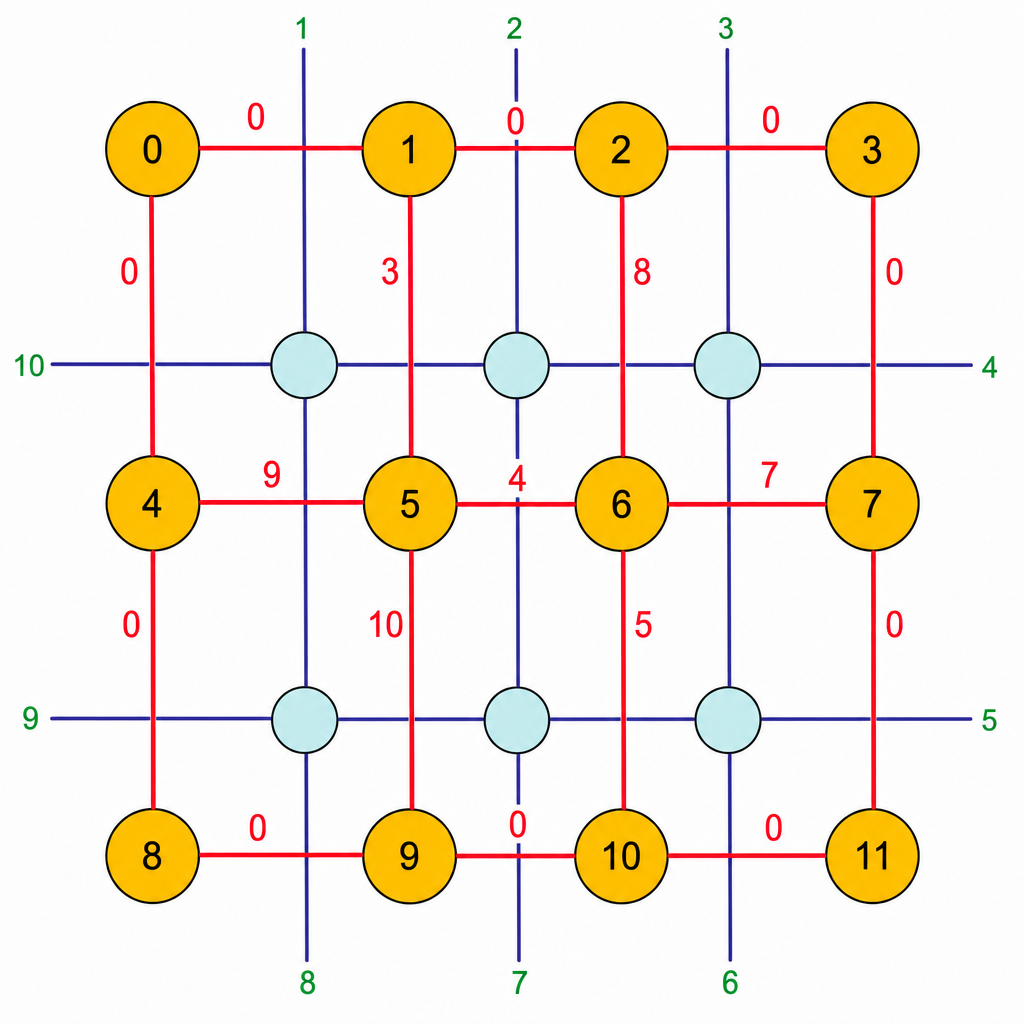
\includegraphics[
        width=0.68\textwidth,
        height=0.34\textheight,
        keepaspectratio
    ]{21-T4/7.png}
\end{figure}

\par\medskip
\noindent\textbf{边界分组}
\par\medskip

当两个不同颜色的附加点分别在射线 $p$ 和射线 $q$ 上时，它们会把整个外边界分成两段。于是，对偶图中的外层点也被分成了两组。

一条合法的割线必须把这两个不同颜色的附加点隔开，所以在对偶图中，它就变成了从第一组外层点到第二组外层点的一条路径。路径越短，割掉的原图边权和越小。

在样例中，两个不同颜色的附加点分别位于射线 $3$ 和射线 $9$。它们把外层点分成两组，我们只需求这两组之间的最短路，可以得到最短距离为 $12$。

\begin{figure}[!htbp]
    \centering
    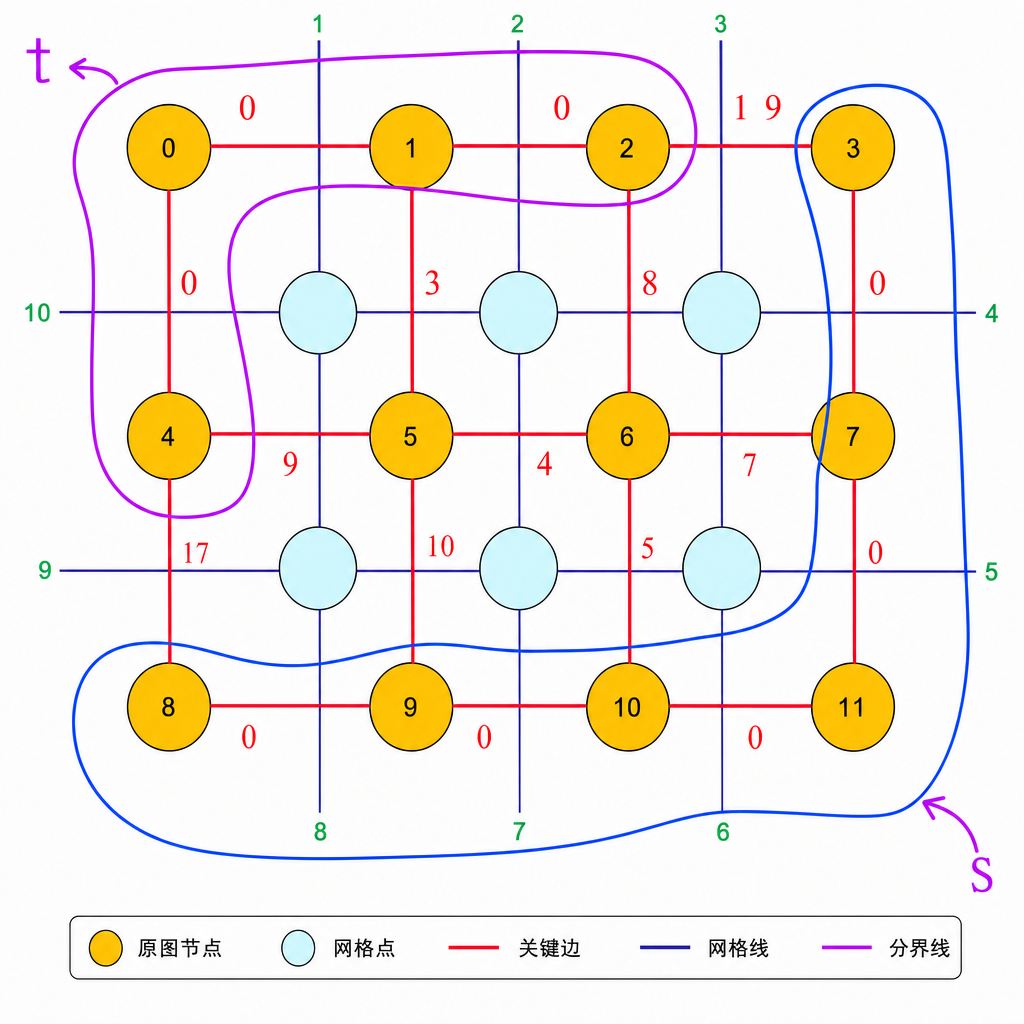
\includegraphics[
        width=0.68\textwidth,
        height=0.34\textheight,
        keepaspectratio
    ]{21-T4/8.png}
\end{figure}

\begin{examplebox}{样例中的最短路含义}
图中从一组外层点走到另一组外层点的最短路长度为 $12$。

这表示在原图中至少要割掉总代价为 $12$ 的边，才能把两个不同颜色的附加点隔开。因此样例答案为 $12$。
\end{examplebox}

如果两个附加点的位置换成射线 $4$ 和射线 $6$，外层点的分组会随之改变，对应的最短路起点集合和终点集合也会改变。如下图所示。

\begin{figure}[!htbp]
    \centering
    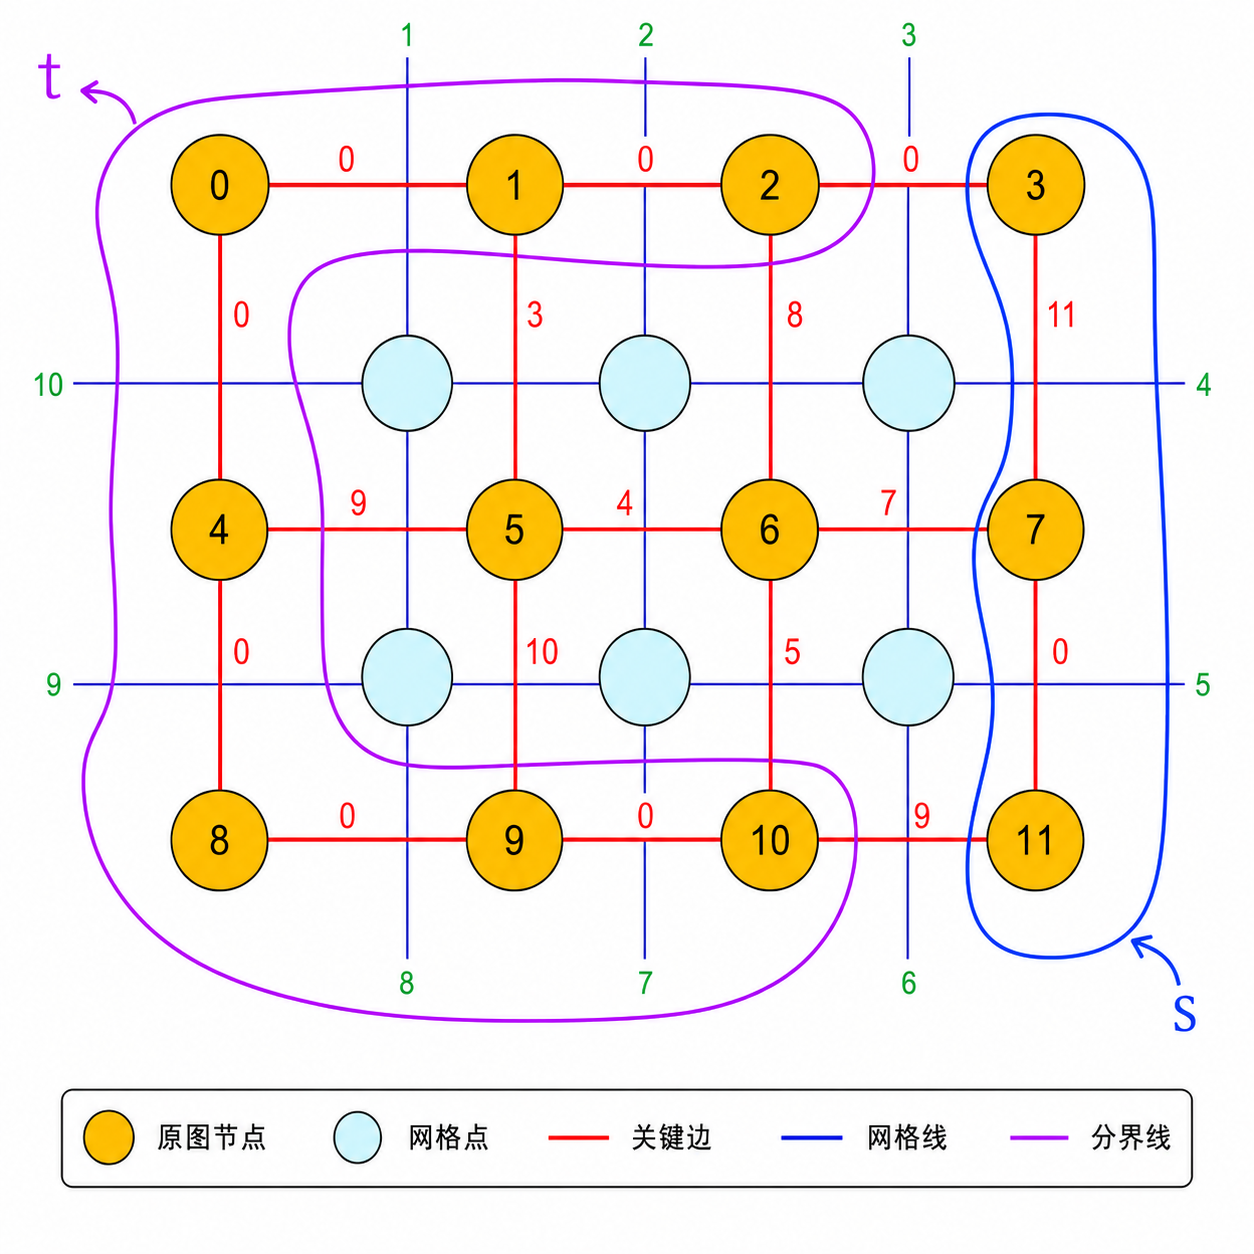
\includegraphics[
        width=0.68\textwidth,
        height=0.34\textheight,
        keepaspectratio
    ]{21-T4/9.png}
\end{figure}

\newpage

\par\medskip
\noindent\textbf{算法步骤}
\par\medskip

\begin{enumerate}[leftmargin=2em,itemsep=1pt,topsep=2pt,parsep=0pt,partopsep=0pt]
    \item 建出原网格对应的对偶图；
    \item 将附加边权加入对偶图的外圈边；
    \item 若 $k_i=1$，或者 $k_i=2$ 且两个附加点颜色相同，直接输出 $0$；
    \item 否则，根据两个射线位置，把外层对偶点分成两组；
    \item 从第一组外层点出发跑多源 Dijkstra，求到第二组外层点的最短距离。
\end{enumerate}

对偶图规模为 $O(nm)$，一次 Dijkstra 的复杂度为 $O(nm\log(nm))$。因此这一做法可以通过所有 $k_i\le 2$ 的数据。

\begin{lstlisting}[style = code]
#include <bits/stdc++.h>
using namespace std;
typedef long long ll;
typedef pair<ll, int> pir;
const ll INF = (ll)4e18;
int main() {
    int n, m, T;
    cin >> n >> m >> T;
    auto id = [&](int i, int j) { return i * (m + 1) + j; };
    vector<vector<int>> down(n, vector<int>(m + 1));
    vector<vector<int>> right(n + 1, vector<int>(m));
    for (int i = 1; i < n; i++)
        for (int j = 1; j <= m; j++) cin >> down[i][j];
    for (int i = 1; i <= n; i++)
        for (int j = 1; j < m; j++) cin >> right[i][j];
    int tot_ray = 2 * (n + m), node_cnt = (n + 1) * (m + 1);
    vector<int> pos(tot_ray + 1);
    for (int p = 1; p <= tot_ray; p++) {
        if (p <= m) pos[p] = id(0, p - 1);
        else if (p <= m + n) pos[p] = id(p - m - 1, m);
        else if (p <= 2 * m + n) pos[p] = id(n, 2 * m + n + 1 - p);
        else pos[p] = id(2 * m + 2 * n + 1 - p, 0);
    }
    auto get_part = [&](int l, int r) {
        vector<int> part;
        if (l < r) {
            for (int p = l + 1; p <= r; p++) part.push_back(pos[p]);
        } else {
            for (int p = l + 1; p <= tot_ray; p++) part.push_back(pos[p]);
            for (int p = 1; p <= r; p++) part.push_back(pos[p]);
        }
        return part;
    };
    while (T--) {
        int k; cin >> k;
        vector<int> p(k), col(k), cost(tot_ray + 1, 0);
        for (int i = 0, val; i < k; i++) {
            cin >> val >> p[i] >> col[i];
            cost[p[i]] = val;
        }
        if (k == 1 || col[0] == col[1]) {
            cout << 0 << '\n'; continue;
        }
        vector<vector<pir>> g(node_cnt);
        auto add_edge = [&](int u, int v, int w) {
            g[u].push_back({v, w}), g[v].push_back({u, w});
        };
        for (int i = 1; i < n; i++)
            for (int j = 1; j <= m; j++)
                add_edge(id(i, j - 1), id(i, j), down[i][j]);
        for (int i = 1; i <= n; i++)
            for (int j = 1; j < m; j++)
                add_edge(id(i - 1, j), id(i, j), right[i][j]);
        for (int x = 1; x <= tot_ray; x++) {
            if (x <= m) add_edge(pos[x], pos[x] + 1, cost[x]);
            else if (x <= m + n) add_edge(pos[x], pos[x] + m + 1, cost[x]);
            else if (x <= 2 * m + n) add_edge(pos[x], pos[x] - 1, cost[x]);
            else add_edge(pos[x], pos[x] - m - 1, cost[x]);
        }
        if (p[0] > p[1]) swap(p[0], p[1]);
        vector<int> s1 = get_part(p[0], p[1]), s2 = get_part(p[1], p[0]);
        vector<ll> dis(node_cnt, INF);
        priority_queue<pir, vector<pir>, greater<pir>> q;
        for (int u : s1) dis[u] = 0, q.push({0, u});
        while (!q.empty()) {
            auto [d, u] = q.top();q.pop();
            if (d != dis[u]) continue;
            for (auto [v, w] : g[u]) 
                if (dis[v] > d + w) dis[v] = d + w, q.push({dis[v], v});
        }
        ll ans = INF;
        for (int u : s2) ans = min(ans, dis[u]);
        cout << ans << '\n';
    }
}
\end{lstlisting}

\newpage
\subsection{满分解法}

前面 $k_i\le 2$ 的做法中，两个不同颜色的附加点会把外边界分成两段，答案就是对偶图中两段外层点之间的一条最短分界线。

当 $k_i$ 变大时，外边界上可能出现多次颜色变化，此时一条分界线已经不够用了。我们需要把边界上真正有影响的位置压缩出来，再处理这些边界段之间的匹配关系。

\par\medskip
\noindent\textbf{第一步：只保留颜色变化的边界段}
\par\medskip

沿着外边界顺时针扫描所有附加点。若相邻两个附加点颜色相同，那么它们之间不需要被割线分开；真正需要处理的是相邻两个附加点颜色不同的位置。

我们把颜色发生变化的边界段压缩成若干块：

\begin{itemize}[leftmargin=2em,itemsep=1pt,topsep=2pt,parsep=0pt,partopsep=0pt]
    \item 从白点走到黑点的边界段记为 $A$ 类；
    \item 从黑点走到白点的边界段记为 $B$ 类。
\end{itemize}

这样，外边界上会交替出现若干个 $A$ 块和 $B$ 块。

\begin{figure}[!htbp]
    \centering
    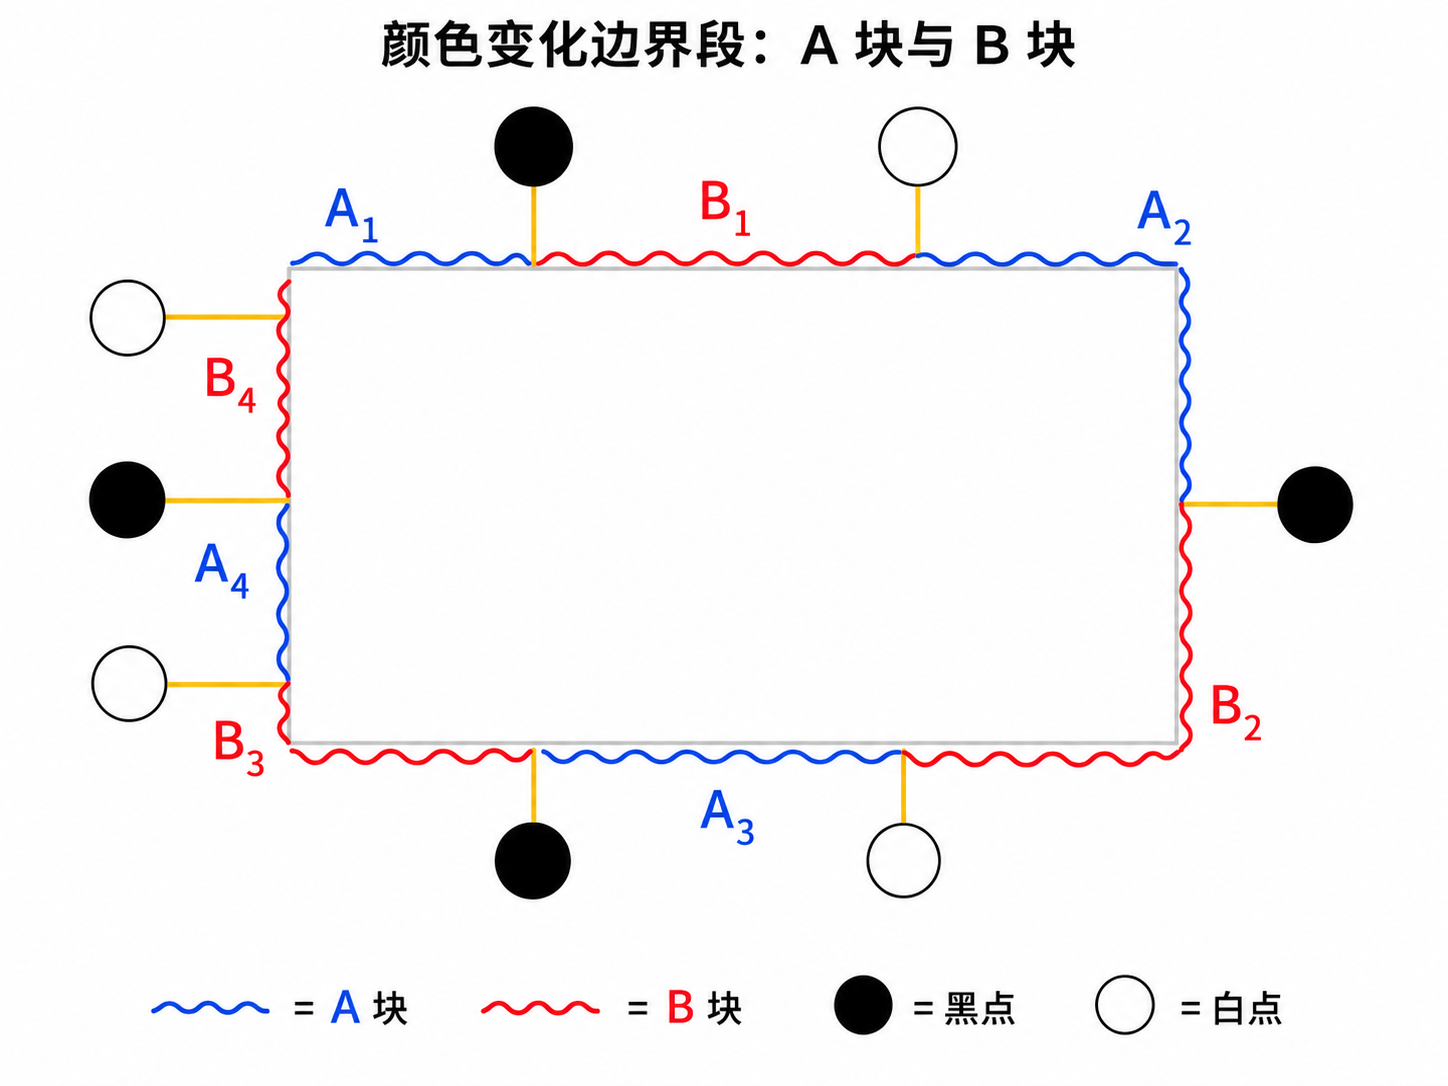
\includegraphics[
        width=0.88\textwidth,
        height=0.36\textheight,
        keepaspectratio
    ]{21-T4/10.png}
\end{figure}

\begin{keybox}{关键观察：只需要关心颜色变化段}
如果一段边界两端对应的附加点颜色相同，那么这一段不会要求割线从这里出发。

只有从黑到白、或从白到黑的边界变化段，才会成为某条割线的端点。
\end{keybox}

若整圈扫描下来没有颜色变化，说明所有附加点颜色相同，此时把所有网格点染成同一种颜色即可，答案为 $0$。
\par\medskip
\noindent\textbf{第二步：割线连接 $A$ 块与 $B$ 块}
\par\medskip

每一条割线的作用，都是把黑色附加点和白色附加点隔开。观察边界变化的方向可以发现，一条割线必须从一个 $A$ 类边界段出发，最终到达一个 $B$ 类边界段。

如果一条线连接两个 $A$ 块，或者连接两个 $B$ 块，那么它并不能正确完成一次颜色区域的切换。

\begin{figure}[!htbp]
    \centering
    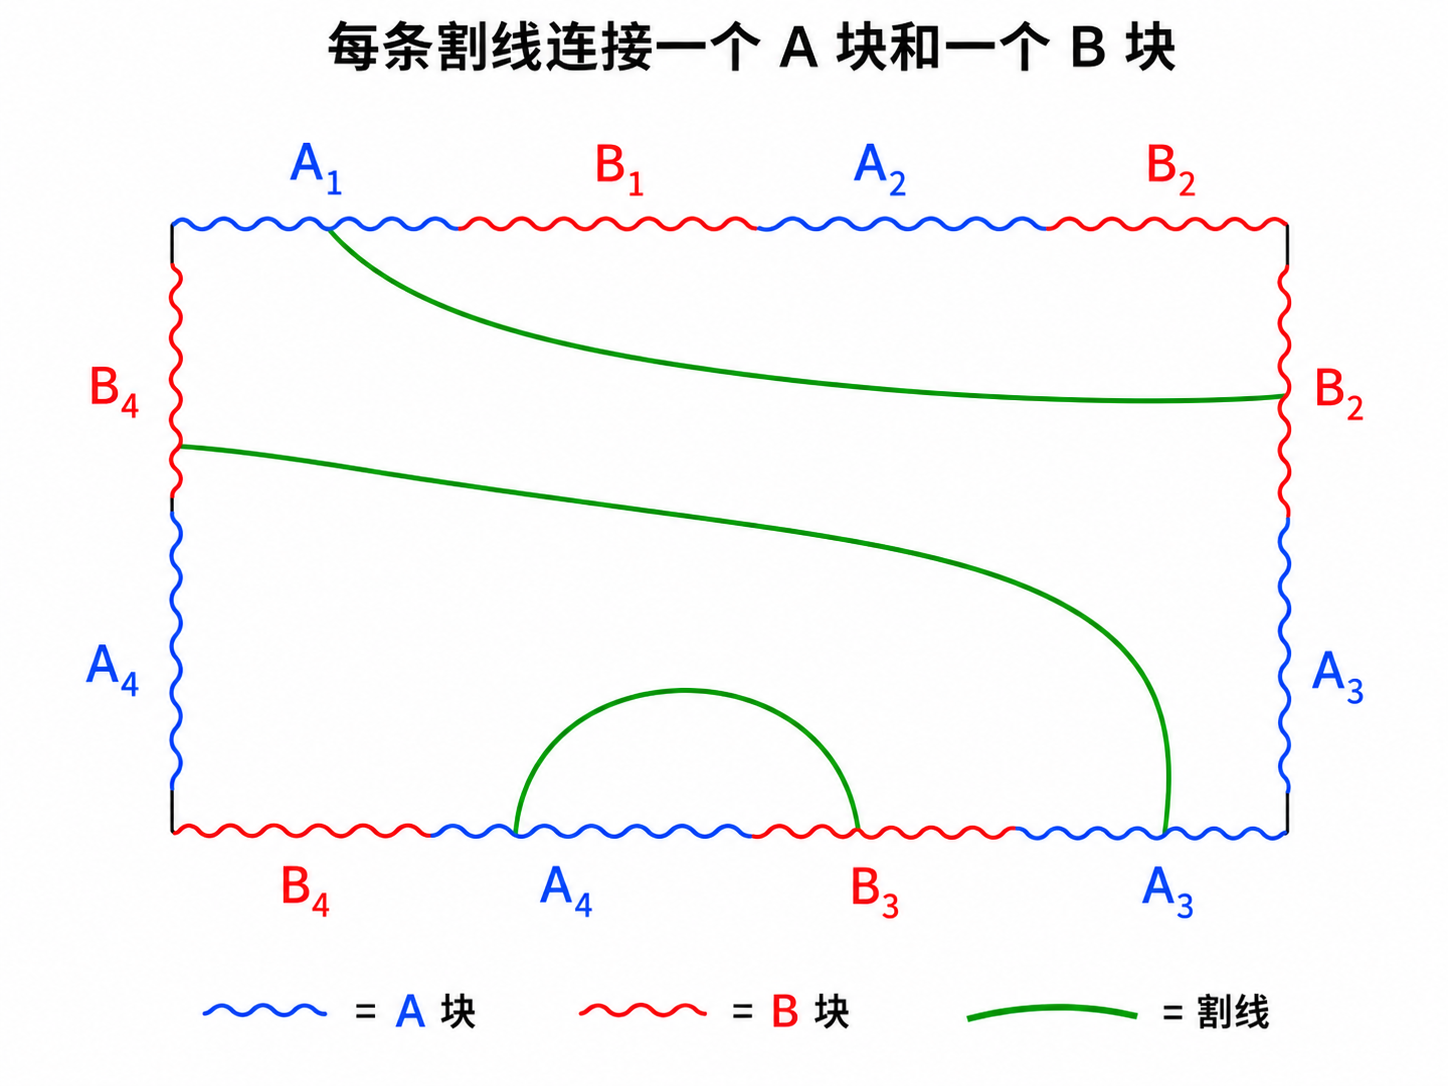
\includegraphics[
        width=0.75\textwidth,
        height=0.25\textheight,
        keepaspectratio
    ]{21-T4/11.png}
\end{figure}

因此，问题可以理解成：在若干个 $A$ 块和 $B$ 块之间连若干条割线，使得所有颜色变化都被处理，并且总代价最小。

这里每一条割线的代价，仍然可以通过对偶图最短路得到。设第 $i$ 个边界块到第 $j$ 个边界块之间的最小代价为 $w_{i,j}$，则

$$
w_{i,j}=\min_{u\in S_i,\ v\in S_j}\mathrm{dist}(u,v)
$$

其中 $S_i,S_j$ 分别表示两个边界块对应的外层对偶点集合，$\mathrm{dist}(u,v)$ 表示对偶图中的最短路长度。

\par\medskip
\noindent\textbf{第三步：最优割线可以看成非交叉匹配}
\par\medskip

如果任意连线，就可能出现两条割线相交的情况。但在平面图中，交叉并不是必要的。

\begin{keybox}{关键观察：存在一组最优的非交叉方案}
若两条割线相交，可以交换它们交点之后的部分，使得连接关系变为不交叉。

这个调整不会增加总长度，同时减少了交叉次数。因此，总存在一组最优方案，使得所有割线两两不交叉。
\end{keybox}

下图左侧表示交叉匹配，右侧表示将其调整为不交叉后的形式。这个性质正是后面使用区间 DP 的原因。

\begin{figure}[!htbp]
    \centering
    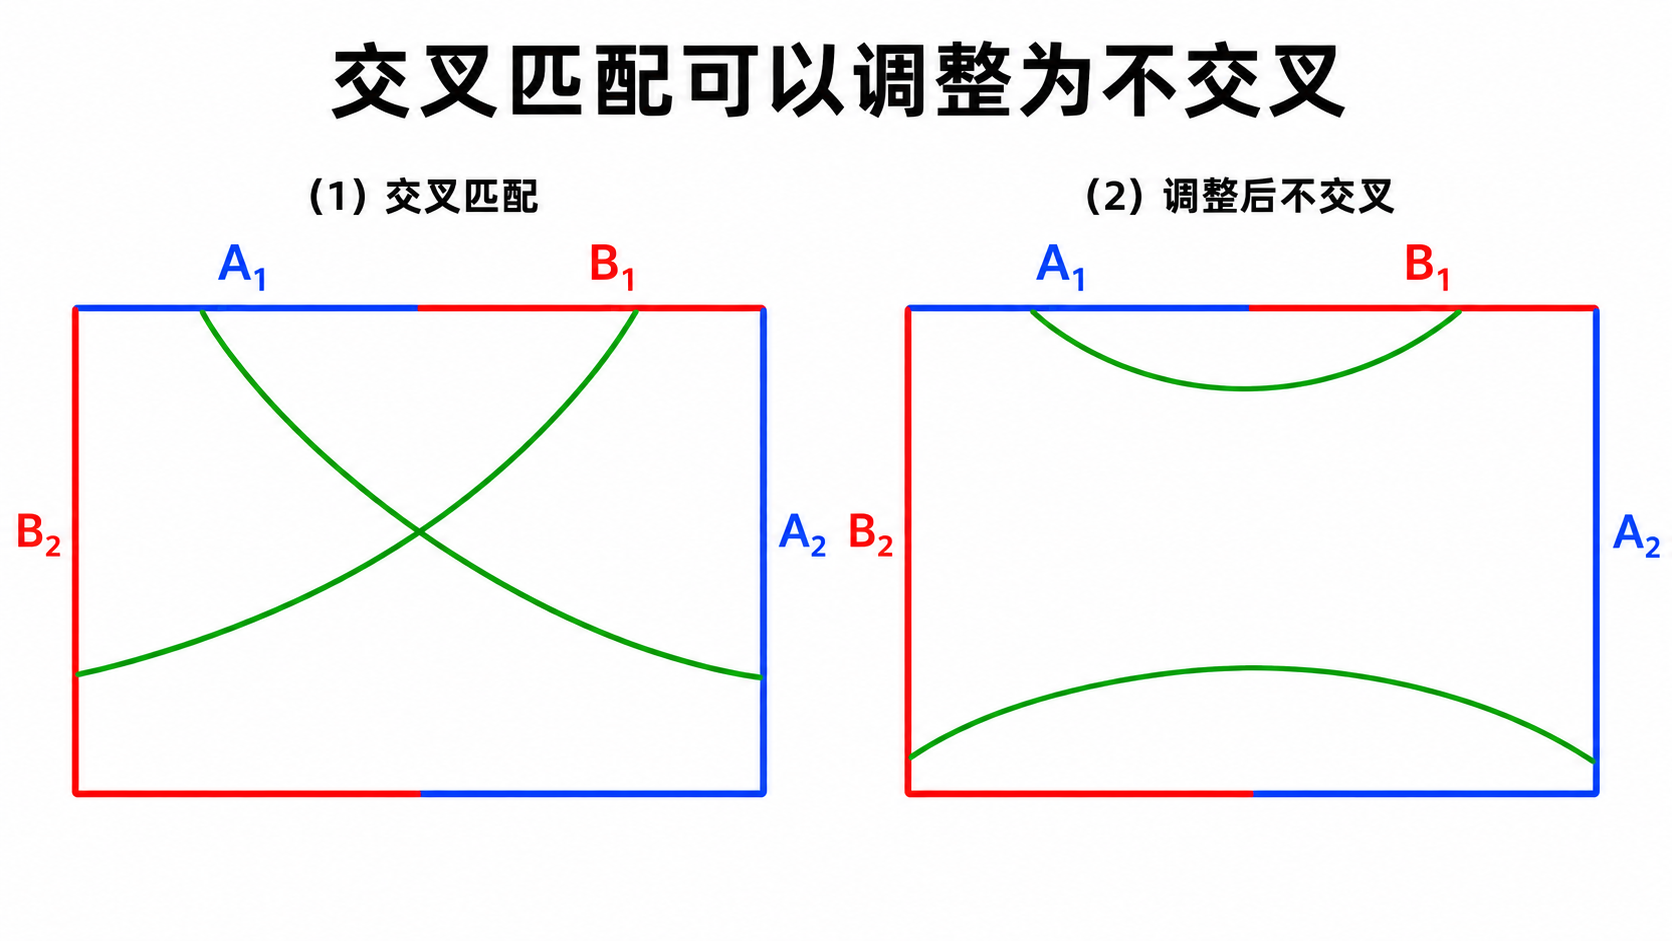
\includegraphics[
        width=0.75\textwidth,
        height=0.22\textheight,
        keepaspectratio
    ]{21-T4/12.png}
\end{figure}

这样一来，满分问题就从“在图上找很多条割线”，转化成了一个更熟悉的问题：

\begin{center}
在环上有若干个交替出现的 $A/B$ 块，将它们两两匹配，要求匹配线不交叉且总代价最小。
\end{center}

\par\medskip
\noindent\textbf{第四步：预处理块之间的最短路}
\par\medskip

设颜色变化后得到的块数为 $c$。由于 $A$ 块和 $B$ 块交替出现，所以 $c$ 一定是偶数。

我们只需要对其中一类块跑 Dijkstra。比如对所有奇数编号的块跑多源 Dijkstra，就可以求出它到所有其他块的最短路代价，从而得到 $w_{i,j}$。

因为 $k_i\le 50$，所以颜色变化块的数量也不超过 $50$。每次询问最多只需要跑 $25$ 次 Dijkstra。

\par\medskip
\noindent\textbf{第五步：断环成链，做区间 DP}
\par\medskip

边界块原本在一个环上。为了方便做区间 DP，我们把环复制一遍，变成长度为 $2c$ 的序列。

令 $f[l][r]$ 表示将区间 $[l,r]$ 内的所有块完成非交叉匹配的最小代价。由于每条匹配连接一个 $A$ 块和一个 $B$ 块，所以只有区间长度为偶数时才有意义。

转移有两种：

\begin{itemize}[leftmargin=2em,itemsep=1pt,topsep=2pt,parsep=0pt,partopsep=0pt]
    \item 将左右端点 $l,r$ 直接匹配，剩下部分为 $[l+1,r-1]$；
    \item 将区间拆成两个互不影响的子区间。
\end{itemize}

核心转移为：

$$
f[l][r]=\min\left(
f[l+1][r-1]+w_{l,r},\
\min_{x}\{f[l][x]+f[x+1][r]\}
\right)
$$

其中 $x$ 只枚举能使左右两段长度均为偶数的位置。

下图展示了“先预处理 $w_{i,j}$，再断环成链做区间 DP”的整体过程。

\begin{figure}[!htbp]
    \centering
    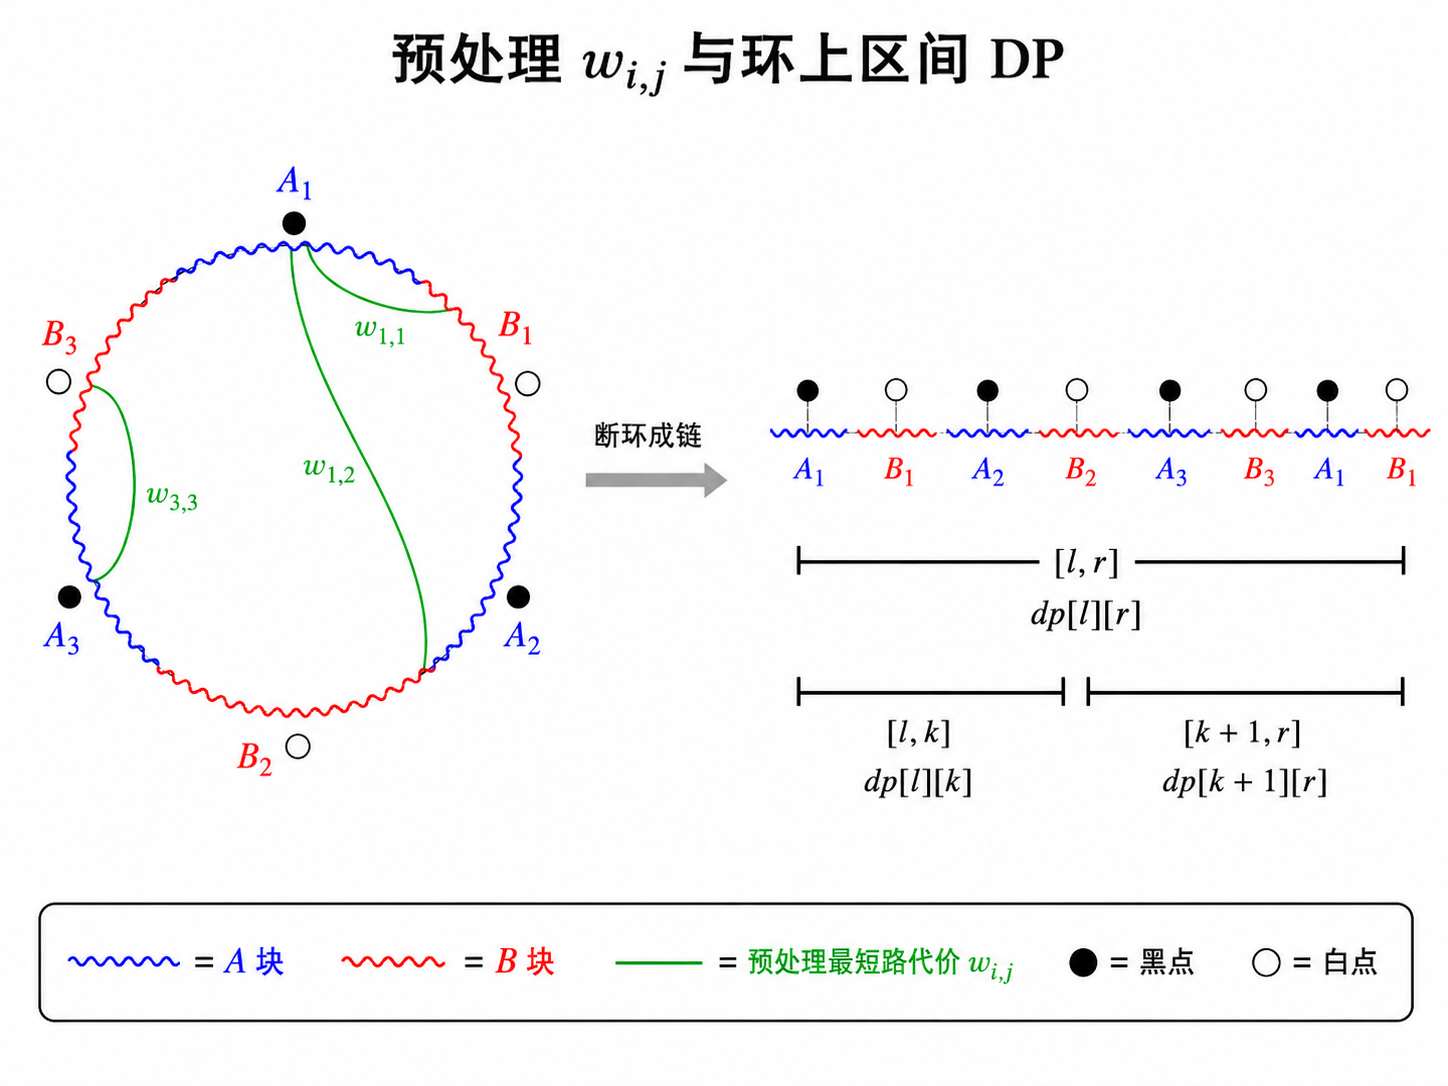
\includegraphics[
        width=0.88\textwidth,
        height=0.32\textheight,
        keepaspectratio
    ]{21-T4/13.png}
\end{figure}

最后答案就是在复制后的序列中，取任意长度为 $c$ 的连续区间的最小值：

$$
ans=\min_{1\le i\le c} f[i][i+c-1]
$$

设一次询问中颜色变化块的数量为 $c$。对偶图规模为 $O(nm)$，每次 Dijkstra 的复杂度为 $O(nm\log(nm))$，最多需要跑 $\frac{c}{2}$ 次；区间 DP 的复杂度为 $O(c^3)$。因此所有询问的总复杂度可以写成
\[
O\left(\sum \frac{c_i}{2}\cdot nm\log(nm)+\sum c_i^3\right).
\]


\begin{lstlisting}[style = code]
int main() {
    // 上面的内容跟 k=2 一致
    while (T--) {
        int k; cin >> k;
        vector<int> color(tot_ray + 1, -1), cost(tot_ray + 1, 0);
        for (int i = 1, val, p, col; i <= k; i++) {
            cin >> val >> p >> col;
            cost[p] = val, color[p] = col;
        }
        vector<vector<pair<int, int>>> g(node_cnt);
        auto add_edge = [&](int u, int v, int w) {
            g[u].push_back({v, w}), g[v].push_back({u, w});
        };
        for (int i = 1; i < n; i++)
            for (int j = 1; j <= m; j++)
                add_edge(id(i, j - 1), id(i, j), down[i][j]);
        for (int i = 1; i <= n; i++)
            for (int j = 1; j < m; j++)
                add_edge(id(i - 1, j), id(i, j), right[i][j]);
        for (int x = 1; x <= tot_ray; x++) {
            if (x <= m) add_edge(pos[x], pos[x] + 1, cost[x]);
            else if (x <= m + n) add_edge(pos[x], pos[x] + m + 1, cost[x]);
            else if (x <= 2 * m + n) add_edge(pos[x], pos[x] - 1, cost[x]);
            else add_edge(pos[x], pos[x] - m - 1, cost[x]);
        }
        vector<vector<int>> seg;
        int first = 0, last = 0;
        for (int p = 1; p <= tot_ray; p++) {
            if (color[p] == -1) continue;
            if (!first) first = p;
            else if (color[last] != color[p]) 
                seg.push_back(get_part(last, p));
            last = p;
        }
        if (first && color[last] != color[first])
            seg.push_back(get_part(last, first));
        int cnt = seg.size();
        if (cnt == 0) { cout << 0 << '\n'; continue; }
        vector<ll> dis(node_cnt);
        auto dijkstra = [&](const vector<int>& src) {
            fill(dis.begin(), dis.end(), INF);
            priority_queue<pir, vector<pir>, greater<pir>> q;
            for (int u : src) {
                if (dis[u] == 0) continue;
                dis[u] = 0, q.push({0, u});
            }
            while (!q.empty()) {
                auto [d, u] = q.top(); q.pop();
                if (d != dis[u]) continue;
                for (auto [v, w] : g[u]) 
                    if (dis[v] > d + w) dis[v] = d + w, q.push({dis[v], v});
            }
        };
        vector<vector<ll>> w(cnt + 1, vector<ll>(cnt + 1, INF));
        for (int i = 1; i <= cnt; i += 2) {
            dijkstra(seg[i - 1]);
            for (int j = 1; j <= cnt; j++) {
                for (int u : seg[j - 1]) w[i][j] = min(w[i][j], dis[u]);
                w[j][i] = w[i][j];
            }
        }
        vector<vector<ll>> val(2 * cnt + 2, vector<ll>(2 * cnt + 2, INF));
        for (int i = 1; i <= 2 * cnt; i++)
            for (int j = 1; j <= 2 * cnt; j++)
                val[i][j] = w[(i - 1) % cnt + 1][(j - 1) % cnt + 1];
        vector<vector<ll>> dp(2 * cnt + 2, vector<ll>(2 * cnt + 2, 0));
        for (int len = 2; len <= cnt; len += 2) {
            for (int l = 1; l + len - 1 <= 2 * cnt; l++) {
                int r = l + len - 1;
                dp[l][r] = dp[l + 1][r - 1] + val[l][r];
                for (int mid = l + 1; mid < r; mid += 2) 
                    dp[l][r] = min(dp[l][r], dp[l][mid] + dp[mid + 1][r]);
            }
        }
        ll ans = INF;
        for (int i = 1; i <= cnt; i++) ans = min(ans, dp[i][i + cnt - 1]);
        cout << ans << '\n';
    }
}
\end{lstlisting}
\chapter{2022 CSP-S复赛解析}
\newpage

\section{T1. 假期计划}

\subsection{题意简析}

给定一张 $n$ 个点、$m$ 条边的无向图，其中 $1$ 号点是家，其余点是景点，每个景点有一个分数。

一次行程最多可以转车 $k$ 次，也就是最多走 $k+1$ 条边。现在要选择四个不同的景点 $A,B,C,D$，使得行程
$1\to A\to B\to C\to D\to 1$ 中每一段都满足转车限制，并最大化四个景点的分数之和。

\subsection{从题面到模型}

这道题表面上是在规划一条包含四个景点的路线，但真正需要关心的只有两件事：

\begin{enumerate}[leftmargin=2em,itemsep=1pt,topsep=2pt,parsep=0pt,partopsep=0pt]
    \item 某两点之间能否在转车限制内到达；
    \item 在满足可达性的前提下，如何让四个景点的分数和最大。
\end{enumerate}

注意，最多转车 $k$ 次，等价于最多经过 $k+1$ 条边。为了叙述方便，记
\[
\mathrm{lim}=k+1.
\]

于是原题可以改写成：

\begin{enumerate}[leftmargin=2em,itemsep=1pt,topsep=2pt,parsep=0pt,partopsep=0pt]
    \item 先预处理任意两点之间的最短路边数；
    \item 把“这一段行程是否合法”统一转化成“最短路边数是否不超过 $\mathrm{lim}$”；
    \item 再在所有满足
    \[
    1\to A,\ A\to B,\ B\to C,\ C\to D,\ D\to 1
    \]
    都合法的四元组中，最大化 $s_A+s_B+s_C+s_D$。
\end{enumerate}

\begin{keybox}{关键转化：中间怎么走不重要，重要的是两点是否可达}
题目并不关心一段路线中途经过了哪些点，只关心这一段能否在转车限制内完成。

因此，先把“路线问题”转化成“点对可达性问题”，后面的优化才有统一的抓手。
\end{keybox}

\subsection{Case 1--8：直接枚举四个景点}

\textbf{部分分特点}：$n\le 20$。

题目给定一张无向图，$1$ 号点是家，其余点是景点。我们需要选择四个不同的景点 $A,B,C,D$，使得路线
$1\to A\to B\to C\to D\to 1$ 中每一段都能在最多 $k$ 次转车内完成，并最大化四个景点的分数之和。

比较直接的做法是：从每个点出发跑一次 \code{BFS}，求出任意两点之间的最短路边数，然后直接枚举 $A,B,C,D$，判断五段路是否合法。

这一做法的复杂度为 $O(n(n+m)+n^4)$，可以通过 $n\le 20$ 的数据。

\begin{lstlisting}[style = code]
#include <bits/stdc++.h>
using namespace std;
typedef long long ll;
const int N = 2505;
int n, m, k, lim, dis[N][N];
ll s[N], ans;
vector<int> g[N];
bool ok(int u, int v) {return dis[u][v] != -1 && dis[u][v] <= lim;}
void bfs(int st) {
    queue<int> q;
    dis[st][st] = 0, q.push(st);
    while (!q.empty()) {
        int u = q.front();
        q.pop();
        if (dis[st][u] == lim) continue;
        for (int v : g[u]) {
            if (dis[st][v] != -1) continue;
            dis[st][v] = dis[st][u] + 1, q.push(v);
        }
    }
}
int main() {
    cin >> n >> m >> k;
    lim = k + 1;
    for (int i = 2; i <= n; i++) cin >> s[i];
    memset(dis, -1, sizeof(dis));
    for (int i = 1; i <= m; i++) {
        int u, v;
        cin >> u >> v;
        g[u].push_back(v);
        g[v].push_back(u);
    }
    for (int i = 1; i <= n; i++) bfs(i);
    for (int a = 2; a <= n; a++) {
        for (int b = 2; b <= n; b++) {
            for (int c = 2; c <= n; c++) {
                for (int d = 2; d <= n; d++) {
                    if (a == b || a == c || a == d) continue;
                    if (b == c || b == d || c == d) continue;
                    if (!ok(1, a) || !ok(a, b) || !ok(b, c)) continue;
                    if (!ok(c, d) || !ok(d, 1)) continue;
                    ans = max(ans, s[a] + s[b] + s[c] + s[d]);
                }
            }
        }
    }
    cout << ans << '\n';
}
\end{lstlisting}

\subsection{Case 1--14：枚举前三个景点}

\textbf{部分分特点}：$n\le 300$。

上一部分的瓶颈在于枚举了四个景点 $A,B,C,D$，复杂度是 $O(n^4)$。现在我们尝试少枚举一个点。

仍然考虑路线：

$$
1\to A\to B\to C\to D\to 1
$$

如果已经枚举了前三个景点 $A,B,C$，那么最后一个景点 $D$ 只需要满足：

\begin{itemize}[leftmargin=2em,itemsep=1pt,topsep=2pt,parsep=0pt,partopsep=0pt]
    \item $C\to D$ 合法；
    \item $D\to 1$ 合法；
    \item $D$ 与 $A,B,C$ 都不同。
\end{itemize}

于是可以对每个景点 $x$，提前预处理所有能作为最后一个景点的候选点 $p$。也就是说，$p$ 需要满足 $\mathrm{ok}(x,p)$ 且 $\mathrm{ok}(p,1)$。

之后把这些候选点按分数从大到小排序。枚举到 $A,B,C$ 后，从 $C$ 的候选列表里找第一个不等于 $A,B,C$ 的点，就是当前情况下最优的 $D$。

\begin{keybox}{为什么只需要检查前三个候选点}
在枚举 $A,B,C$ 后，候选点 $D$ 只可能因为与 $A,B,C$ 重复而不能选。

又因为预处理 $C$ 的候选列表时已经排除了 $D=C$ 的情况，所以实际上最多只会被 $A,B$ 两个点排除。因此检查分数最大的前三个候选点就足够了。
\end{keybox}

这一做法的复杂度为 $O(n(n+m)+n^3)$，可以通过 $n\le 300$ 的数据。

\newpage
\begin{lstlisting}[style = code]
// ... 主函数上面的内容跟 case 1~8 一致
vector<int> cand[N];
int main() {
    // ... 输入部分跟 case 1~8 一致
    memset(dis, -1, sizeof(dis));
    for (int i = 1; i <= n; i++) bfs(i);
    // cand[x]: 可以作为 x -> p -> 1 中 p 的候选点
    for (int x = 2; x <= n; x++) {
        for (int p = 2; p <= n; p++) {
            if (x == p) continue;
            if (ok(x, p) && ok(p, 1)) cand[x].push_back(p);
        }
        sort(cand[x].begin(), cand[x].end(), [&](int u, int v) {
            return s[u] > s[v];
        });
    }
    for (int a = 2; a <= n; a++) {
        for (int b = 2; b <= n; b++) {
            for (int c = 2; c <= n; c++) {
                for (int t = 0; t < min(3, (int)cand[c].size()); t++) {
                    int d = cand[c][t];
                    if (a == b || a == c || a == d) continue;
                    if (b == c || b == d || c == d) continue;
                    if (!ok(1, a) || !ok(a, b) || !ok(b, c)) continue;
                    if (!ok(c, d) || !ok(d, 1)) continue;
                    ans = max(ans, s[a] + s[b] + s[c] + s[d]);
                }
            }
        }
    }
    cout << ans << '\n';
}
\end{lstlisting}
\newpage
\subsection{满分解法：枚举中间两个景点}

\textbf{部分分特点}：$n\le 2500$。

在上一部分中，我们枚举了 $A,B,C$，然后快速选择最优的 $D$。满分做法继续沿用这个思路：既然最后一个点可以通过候选列表优化，那么第一个点也可以一并提前处理。

考虑固定中间两个景点 $B,C$。路线变为：

$$
1\to A\to B\to C\to D\to 1
$$

此时：

\begin{itemize}[leftmargin=2em,itemsep=1pt,topsep=2pt,parsep=0pt,partopsep=0pt]
    \item $A$ 需要满足 $1\to A$ 合法，且 $A\to B$ 合法；
    \item $D$ 需要满足 $C\to D$ 合法，且 $D\to 1$ 合法；
    \item $A,B,C,D$ 两两不同。
\end{itemize}

由于图是无向图，$C\to D$ 合法等价于 $D\to C$ 合法。于是我们可以统一预处理“能放在某个点前面的候选点”。

具体来说，对于每个景点 $x$，我们维护若干个候选点 $p$。如果 $1\to p$ 合法，且 $p\to x$ 合法，那么 $p$ 就可以放在 $x$ 的前一站。

这样一来，枚举中间两个景点 $B,C$ 时，$B$ 的候选点可以作为 $A$，$C$ 的候选点可以作为 $D$。

这个候选点思想在上一部分已经出现过。现在我们只需要对每个点保留分数最大的前三个候选点，然后枚举中间两个景点 $B,C$ 即可。

\begin{keybox}{为什么每个点只保留前三个候选点就够了}
固定中间两个景点 $B,C$ 后，候选点 $A$ 只可能因为与 $B,C,D$ 重复而不能选，候选点 $D$ 也只可能因为与 $A,B,C$ 重复而不能选。

也就是说，对某一侧的候选列表来说，真正会把“分数最高的候选点”排除掉的不同景点数量至多只有 $3$ 个。于是只保留每个列表中分数最高的前三个候选点，就已经足够覆盖所有可能成为最优解的情况。
\end{keybox}

\begin{keybox}{从枚举三个点优化到枚举两个点}
上一部分固定 $A,B,C$ 后，只从 $C$ 的候选列表中选 $D$。

满分做法则固定 $B,C$，同时从 $B$ 的候选列表中选 $A$，从 $C$ 的候选列表中选 $D$。这样就把枚举量从 $O(n^3)$ 降到了 $O(n^2)$。
\end{keybox}

算法流程如下：

\begin{enumerate}[leftmargin=2em,itemsep=1pt,topsep=2pt,parsep=0pt,partopsep=0pt]
    \item 从每个点出发跑一次 \code{BFS}，得到任意两点之间的最短路边数；
    \item 对每个景点 $x$，预处理能够作为 $1\to p\to x$ 中 $p$ 的前三优候选点；
    \item 枚举中间两个景点 $B,C$，要求 $B\ne C$ 且 $B\to C$ 合法；
    \item 枚举 $B$ 的前三个候选点作为 $A$，枚举 $C$ 的前三个候选点作为 $D$，检查四个景点是否两两不同，并更新答案。
\end{enumerate}

预处理所有候选列表并排序的复杂度为 $O(n^2\log n)$，枚举中间两个景点时，每组 $(B,C)$ 只需要尝试常数个候选点组合，因此这一部分的复杂度为 $O(n^2)$。综合起来，总时间复杂度为 $O(n(n+m)+n^2\log n)$，可以通过所有数据。

\newpage
\begin{lstlisting}[style = code]
// ... 主函数上面的内容跟 case 1~8 一致
vector<int> cand[N];// cand[x]: 可以作为 x -> p -> 1 中 p 的候选点
int main() {
    // ... 输入部分跟 case 1~8 一致
    memset(dis, -1, sizeof(dis));
    for (int i = 1; i <= n; i++) bfs(i);
    // cand[x]: 可以作为 x -> p -> 1 中 p 的候选点
    for (int x = 2; x <= n; x++) {
        for (int p = 2; p <= n; p++) {
            if (x == p) continue;
            if (ok(x, p) && ok(p, 1)) cand[x].push_back(p);
        }
        sort(cand[x].begin(), cand[x].end(), [&](int u, int v) {
            return s[u] > s[v];
        });
        // 把候选点的数量控制在 3 以内
        if ((int)cand[x].size() > 3) cand[x].resize(3);
    }
    // 枚举中间两个景点 b, c
    for (int b = 2; b <= n; b++) {
        for (int c = 2; c <= n; c++) {
            for (int a : cand[b]) {
                for (int d : cand[c]) {
                    if (a == b || a == c || a == d) continue;
                    if (b == c || b == d || c == d) continue;
                    if (!ok(1, a) || !ok(a, b) || !ok(b, c)) continue;
                    if (!ok(c, d) || !ok(d, 1)) continue;
                    ans = max(ans, s[a] + s[b] + s[c] + s[d]);
                }
            }
        }
    }
    cout << ans << '\n';
}
\end{lstlisting}
\newpage
\section{T2. 策略游戏}
\subsection{题意简析}

给定两个数组 $A$ 和 $B$，定义矩阵 $C$ 满足 $C_{i,j}=A_i\times B_j$。

每次询问给出两个区间 $[l_1,r_1]$ 和 $[l_2,r_2]$。小 L 先从 $A$ 的区间中选择一个下标 $x$，小 Q 再从 $B$ 的区间中选择一个下标 $y$，最终得分为 $A_x\times B_y$。

小 L 希望得分尽可能大，小 Q 希望得分尽可能小。要求输出双方都采取最优策略时，每次询问的最终得分。

\subsection{从题面到模型}

虽然题目中定义了一个矩阵 $C$，但我们并不需要真的建立这个 $n\times m$ 的矩阵。因为每个格子的值都可以直接写成 $A_x\times B_y$。

对于一次询问，小 L 先选择 $x$，小 Q 后选择 $y$。由于小 Q 会在知道 $x$ 的情况下让结果尽量小，所以当 $x$ 固定时，最终得分是：

$$
\min_{y\in [l_2,r_2]} A_xB_y
$$

而小 L 会选择一个最有利的 $x$，因此整次询问要求的是：

$$
\max_{x\in [l_1,r_1]}\min_{y\in [l_2,r_2]} A_xB_y
$$

这样一来，问题就从“在矩阵 $C$ 的某个子矩阵中思考”转化成了“在两个一维区间中，根据乘法符号关系做最优选择”。

\begin{keybox}{关键转化：先固定小 L 的选择，再看小 Q 的最优反应}
这一题的难点不在于乘法本身，而在于双方的先后手顺序。

因此分析时应当先固定 $A$ 中的一个数 $x$，求出小 Q 在 $B$ 区间中的最优反应；再回过头来，让小 L 在所有可能的 $x$ 里挑一个最优解。
\end{keybox}

\newpage
\subsection{Case 1--5：直接枚举双方选择}

\textbf{部分分特点}：$n,m,q\le 200$。

根据上一部分的形式化表达，一次询问的答案是：

$$
\max_{x\in [l_1,r_1]}\min_{y\in [l_2,r_2]} A_xB_y
$$

因此最直接的做法就是按照这个式子模拟。

我们枚举小 L 选择的下标 $x$。当 $x$ 固定后，小 Q 会在 $[l_2,r_2]$ 中枚举所有 $y$，找到最小的 $A_xB_y$。最后小 L 在所有 $x$ 对应的最小值中取最大值。
\begin{lstlisting}[style = code]
#include <bits/stdc++.h>
using namespace std;
typedef long long ll;
const ll N = 205, INF = 1e18;
int n, m, q;
ll a[N], b[N];
int main() {
    cin >> n >> m >> q;
    for (int i = 1; i <= n; i++) cin >> a[i];
    for (int i = 1; i <= m; i++) cin >> b[i];
    while (q--) {
        int l1, r1, l2, r2;
        cin >> l1 >> r1 >> l2 >> r2;
        ll ans = -INF;
        for (int x = l1; x <= r1; x++) {
            ll now = INF;
            for (int y = l2; y <= r2; y++) now = min(now, a[x] * b[y]);
            ans = max(ans, now);
        }
        cout << ans << '\n';
    }
}

\end{lstlisting}

\subsection{特殊性质 1：所有数均为正数}

\textbf{部分分特点}：保证 $A_i,B_i>0$。

在这个特殊性质下，所有参与乘法的数都是正数。

对于固定的 $A_x$，小 Q 想让 $A_xB_y$ 尽量小，就一定会选择 $B$ 区间中的最小值。此时小 L 想让最终得分尽量大，就会选择 $A$ 区间中的最大值。

因此答案就是：

$$
\max(A[l_1\sim r_1])\times \min(B[l_2\sim r_2])
$$
\begin{lstlisting}[style = code]
#include <bits/stdc++.h>
using namespace std;
typedef long long ll;
const int N = 100005, LOG = 20;
struct ST {
    int f[LOG][N];
    bool is_max;
    int merge_val(int x, int y) { return is_max ? max(x, y) : min(x, y);}
    // op = true 表示求解最大值 op = false 表示求解最小值
    void build(int n, bool op) {
        is_max = op;
        for (int j = 1; j < LOG; j++) {
            for (int i = 1; i + (1 << j) - 1 <= n; i++) {
                f[j][i] = merge_val(f[j - 1][i],
                                     f[j - 1][i + (1 << (j - 1))]);
            }
        }
    }
    int query(int l, int r) {
        int k = log2(r - l + 1);
        return merge_val(f[k][l], f[k][r - (1 << k) + 1]);
    }
};
int n, m, q;
int a[N], b[N];
ST st_a_max, st_b_min;
int main() {
    cin >> n >> m >> q;
    for (int i = 1; i <= n; i++) {
        cin >> a[i]; st_a_max.f[0][i] = a[i];
    }
    for (int i = 1; i <= m; i++) {
        cin >> b[i]; st_b_min.f[0][i] = b[i];
    }
    st_a_max.build(n, true), st_b_min.build(m, false);
    while (q--) {
        int l1, r1, l2, r2;
        cin >> l1 >> r1 >> l2 >> r2;
        ll x = st_a_max.query(l1, r1), y = st_b_min.query(l2, r2);
        cout << x * y << '\n';
    }
}
\end{lstlisting}

\subsection{Case 1--12：按符号分类讨论}

\textbf{部分分特点}：$n,m,q\le 1000$。

一般情况下，数组里可能同时出现正数、负数和 $0$。此时就不能只看区间最大值和最小值，而要继续分析小 Q 在 $x$ 固定后的最优反应。

假设小 L 已经选定了一个数 $x=A_x$：
\begin{itemize}[leftmargin=2em,itemsep=1pt,topsep=2pt,parsep=0pt,partopsep=0pt]
    \item 若 $x\ge 0$，为了让 $x\cdot y$ 尽量小，小 Q 会选择 $B$ 区间中的最小值；
    \item 若 $x<0$，乘上负数后大小关系反向，小 Q 会选择 $B$ 区间中的最大值。
\end{itemize}

\begin{keybox}{关键观察：小 Q 的选择只和 $x$ 的符号有关}
记 $B$ 询问区间中的最小值为 $b_{\min}$，最大值为 $b_{\max}$。

如果小 L 选择的数是 $x$，那么这一选择最终会得到：

$$
\begin{cases}
x\cdot b_{\min}, & x\ge 0,\\
x\cdot b_{\max}, & x<0.
\end{cases}
$$

小 L 要做的，就是在 $A$ 的询问区间中选择一个让上述值最大的 $x$。
\end{keybox}

进一步观察，虽然 $A$ 的区间中可能有很多数，但真正有必要考虑的只有少数几类：

\begin{itemize}[leftmargin=2em,itemsep=1pt,topsep=2pt,parsep=0pt,partopsep=0pt]
    \item 区间最大值；
    \item 区间最小值；
    \item 负数中的最大值；
    \item 非负数中的最小值。
\end{itemize}

原因是：对于非负数 $x$，最终得分是 $x\cdot b_{\min}$。如果 $b_{\min}\ge 0$，应该选尽量大的非负数；如果 $b_{\min}<0$，应该选尽量小的非负数。负数的情况同理，只是对应的对象换成了 $b_{\max}$。

因此，在 $n,m,q\le 1000$ 时，可以对每次询问暴力扫描两个区间，求出这些值，再逐一计算候选答案。单次询问复杂度为 $O(n+m)$。
\newpage
\begin{lstlisting}[style = code]
#include <bits/stdc++.h>
using namespace std;
typedef long long ll;
const int N = 1005, INF = 2e9;
int n, m, q;
int a[N], b[N];
ll calc(int x, int b_min, int b_max) {
    if (x >= 0) return 1LL * x * b_min;
    return 1LL * x * b_max;
}
int main() {
    cin >> n >> m >> q;
    for (int i = 1; i <= n; i++) cin >> a[i];
    for (int i = 1; i <= m; i++) cin >> b[i];
    while (q--) {
        int l1, r1, l2, r2;
        cin >> l1 >> r1 >> l2 >> r2;
        int a_max = -INF, a_min = INF;
        int a_neg = -INF, a_nonneg = INF;
        int b_max = -INF, b_min = INF;
        for (int i = l1; i <= r1; i++) {
            a_max = max(a_max, a[i]);
            a_min = min(a_min, a[i]);
            if (a[i] < 0) a_neg = max(a_neg, a[i]);
            else a_nonneg = min(a_nonneg, a[i]);
        }
        for (int i = l2; i <= r2; i++) {
            b_max = max(b_max, b[i]);
            b_min = min(b_min, b[i]);
        }
        ll ans = LLONG_MIN;
        ans = max(ans, calc(a_max, b_min, b_max));
        ans = max(ans, calc(a_min, b_min, b_max));
        if (a_neg != -INF) ans = max(ans, calc(a_neg, b_min, b_max));
        if (a_nonneg != INF) ans = max(ans, calc(a_nonneg, b_min, b_max));
        cout << ans << '\n';
    }
}
\end{lstlisting}
\newpage
\subsection{满分解法：ST 表维护六类最值}

\textbf{部分分特点}：$n,m,q\le 10^5$。

上一部分已经把一次询问转化成了若干类区间最值的查询。瓶颈在于，每次询问都要线性扫描区间，去找这些最大值和最小值。

由于数组不发生修改，这些信息都是静态区间最值，因此可以直接用 ST 表优化。

具体需要维护六个 ST 表：

\begin{itemize}[leftmargin=2em,itemsep=1pt,topsep=2pt,parsep=0pt,partopsep=0pt]
    \item $A$ 的区间最大值；
    \item $A$ 的区间最小值；
    \item $A$ 中负数的区间最大值；
    \item $A$ 中非负数的区间最小值；
    \item $B$ 的区间最大值；
    \item $B$ 的区间最小值。
\end{itemize}

其中，维护 $A$ 中负数最大值时，可以把非负数位置初始化为极小值；维护 $A$ 中非负数最小值时，可以把负数位置初始化为极大值。这样一来，查询时仍然只是普通的区间最大值或最小值。

\begin{keybox}{关键观察：把分类讨论转化为区间最值}
每次询问只需要得到 $A$ 区间中的四类候选数，以及 $B$ 区间中的最大值和最小值。

之后逐一计算每个候选数在小 Q 最优选择下的得分，取最大值，就是小 L 的最优答案。
\end{keybox}

预处理 ST 表复杂度为 $O((n+m)\log(n+m))$，单次询问复杂度为 $O(1)$，因此总复杂度为 $O((n+m)\log(n+m)+q)$，空间复杂度为 $O((n+m)\log(n+m))$。

下面代码中，\code{ST} 结构体与上一节特殊性质 1 中的 ST 表实现相同，不再重复展示。

\begin{lstlisting}[style = code]
// ST 结构体与上一节相同
const int INF = 2000000007;
int n, m, q;
int a[N], b[N];
ST st_a_max, st_a_min, st_a_neg, st_a_nonneg;
ST st_b_max, st_b_min;
ll calc(int x, int b_min, int b_max) {
    if (x >= 0) return 1LL * x * b_min;
    return 1LL * x * b_max;
}
int main() {
    cin >> n >> m >> q;
    for (int i = 1; i <= n; i++) {
        cin >> a[i];
        st_a_max.f[0][i] = a[i];
        st_a_min.f[0][i] = a[i];
        st_a_neg.f[0][i] = (a[i] < 0 ? a[i] : -INF);
        st_a_nonneg.f[0][i] = (a[i] >= 0 ? a[i] : INF);
    }

    for (int i = 1; i <= m; i++) {
        cin >> b[i];
        st_b_max.f[0][i] = b[i];
        st_b_min.f[0][i] = b[i];
    }

    st_a_max.build(n, true);
    st_a_min.build(n, false);
    st_a_neg.build(n, true);
    st_a_nonneg.build(n, false);
    st_b_max.build(m, true);
    st_b_min.build(m, false);

    while (q--) {
        int l1, r1, l2, r2;
        cin >> l1 >> r1 >> l2 >> r2;

        int a_max = st_a_max.query(l1, r1);
        int a_min = st_a_min.query(l1, r1);
        int a_neg = st_a_neg.query(l1, r1);
        int a_nonneg = st_a_nonneg.query(l1, r1);
        int b_max = st_b_max.query(l2, r2);
        int b_min = st_b_min.query(l2, r2);

        ll ans = LLONG_MIN;

        ans = max(ans, calc(a_max, b_min, b_max));
        ans = max(ans, calc(a_min, b_min, b_max));

        if (a_neg != -INF) ans = max(ans, calc(a_neg, b_min, b_max));
        if (a_nonneg != INF) ans = max(ans, calc(a_nonneg, b_min, b_max));
        cout << ans << '\n';
    }
}
\end{lstlisting}
\newpage

\section{T3. 星战}

\subsection{题意简析}

给定一张有 $n$ 个点、$m$ 条边的有向图，每条边都有可用和不可用两种状态，初始时所有边均可用。

接下来有四种操作：删除一条边、删除所有以某点为终点的边、恢复一条边、恢复所有以某点为终点的边。每次操作后，需要判断当前时刻是否可以反攻。

\subsection{从题面到模型}

题目中有两个限制：每个点都要能无限穿梭，并且每个点出发时只能选择唯一一条可用虫洞。后一个限制实际上就是说，每个点当前的可用出度必须恰好为 $1$。

\begin{keybox}{关键观察：只需要判断可用出度}
如果每个点的可用出度都恰好为 $1$，那么从任意点出发，每一步都能继续走向下一个点。由于点数有限，走足够多步以后一定会重复经过某个点，从而进入一个有向环。

因此，“可以无限穿梭”的要求会自动满足。当前时刻能够反攻，当且仅当所有点的可用出度都等于 $1$。
\[
\forall u,\quad deg_u=1
\]
\end{keybox}

这样一来，问题就转化成了：在四种边状态修改操作下，动态维护每个点的可用出度是否都等于 $1$。

\subsection{Case 1--8：直接模拟边状态}

\textbf{部分分特点}：$n,m,q$ 较小。

比较自然的想法是直接维护每条边当前是否可用。令 $deg_u$ 表示点 $u$ 当前的可用出度，再令 $cnt$ 表示当前有多少个点满足 $deg_u=1$。每次修改某个点的出度时，同步维护 $cnt$ 即可。

由于操作 $2$ 和操作 $4$ 都是针对“所有以某点为终点的边”，所以我们按终点存边。也就是说，在 $in_v$ 中保存所有形如 $(u,v)$ 的边。

四种操作的变化如下：

\begin{itemize}[leftmargin=2em,itemsep=1pt,topsep=2pt,parsep=0pt,partopsep=0pt]
    \item 删除边 $(u,v)$：在 $in_v$ 中找到这条边，将其标记为不可用，并令 $deg_u$ 减少 $1$；
    \item 删除所有到 $v$ 的边：枚举 $in_v$ 中所有当前可用的边 $(u,v)$，逐条标记为不可用，并令对应的 $deg_u$ 减少 $1$；
    \item 恢复边 $(u,v)$：在 $in_v$ 中找到这条边，将其标记为可用，并令 $deg_u$ 增加 $1$；
    \item 恢复所有到 $v$ 的边：枚举 $in_v$ 中所有当前不可用的边 $(u,v)$，逐条标记为可用，并令对应的 $deg_u$ 增加 $1$。
\end{itemize}

每次操作后，只需要判断 $cnt=n$。

这种做法的瓶颈在于操作 $2$ 和操作 $4$。一次操作可能枚举大量入边，因此对于大数据无法通过。
\newpage
\begin{lstlisting}[style = code]
#include <bits/stdc++.h>
using namespace std;
typedef pair<int, int> pir;
const int N = 5e5 + 5;
vector<pir> e[N];  // e[v] 存所有指向 v 的边，first 是起点，second 表示是否可用
int out[N], cnt;
void change_out(int u, int delta) {
    if (out[u] == 1) cnt--;
    out[u] += delta;
    if (out[u] == 1) cnt++;
}
int main() {
    int n, m;
    cin >> n >> m;
    for (int i = 1; i <= m; i++) {
        int u, v;
        cin >> u >> v;
        out[u]++;
        e[v].push_back({u, 1});
    }
    for (int i = 1; i <= n; i++) if (out[i] == 1) cnt++;
    int q;
    cin >> q;
    while (q--) {
        int op, u, v;
        cin >> op;
        if (op == 1) {  // 删除 u -> v
            cin >> u >> v;
            change_out(u, -1);
            for (auto &edge : e[v]) {
                if (edge.first == u) {
                    edge.second = 0;
                    break;
                }
            }
        } else if (op == 2) {  // 删除所有到 u 的边
            cin >> u;
            for (auto &edge : e[u]) {
                if (edge.second == 0) continue;
                edge.second = 0;
                change_out(edge.first, -1);
            }
        } else if (op == 3) {  // 恢复 u -> v
            cin >> u >> v;
            change_out(u, 1);
            for (auto &edge : e[v]) {
                if (edge.first == u) {
                    edge.second = 1;
                    break;
                }
            }
        } else {  // 恢复所有到 u 的边
            cin >> u;
            for (auto &edge : e[u]) {
                if (edge.second == 1) continue;
                edge.second = 1;
                change_out(edge.first, 1);
            }
        }
        cout << (cnt == n ? "YES" : "NO") << '\n';
    }
}
\end{lstlisting}

\subsection{Case 9--10：只维护出度}

\textbf{部分分特点}：保证没有操作 $2$ 和操作 $4$。

沿着上一部分的思路继续看，这一档数据中不会出现按终点批量删除或恢复的操作，因此不会遇到“一次操作影响大量起点出度”的问题。

也就是说，只保留 $deg_u$ 和 $cnt$ 的维护即可：

\begin{itemize}[leftmargin=2em,itemsep=1pt,topsep=2pt,parsep=0pt,partopsep=0pt]
    \item 删除边 $(u,v)$ 时，令 $deg_u$ 减少 $1$；
    \item 恢复边 $(u,v)$ 时，令 $deg_u$ 增加 $1$。
\end{itemize}

每次修改前后同步维护 $cnt$，最后判断 $cnt=n$。由于每次操作只影响一个点的出度，所以单次复杂度为 $O(1)$。

按照 Case 1--8 的做法，这部分也能通过；只不过因为没有批量操作，代码中枚举入边的部分不会成为瓶颈。

\newpage
\subsection{满分做法}

我们进一步思考操作 $2$ 和 $4$，可以发现：比起维护出度，其实更容易的是维护入度。

对于这两个操作而言，如果我们执行操作 $2$，实际上就是把这个点的入度直接变成 $0$；执行操作 $4$，就是把这个点的入度恢复成初始最大值，而这个最大值也是容易维护的。这样一来，入度层面的变化就都可以在常数时间内完成。

对于一个图而言，每一条边会同时贡献一个出度和一个入度，所以总入度永远等于总出度。但是这里存在一个问题：即使总入度等于 $n$，也不能推出“每个点的入度都恰好为 $1$”。

\begin{keybox}{关键观察：用哈希增强必要条件}
“总入度为 $n$”只是每个点入度都为 $1$ 的必要条件，但我们可以利用\textbf{随机哈希}把这个必要条件强化成一个极高概率正确的判据。

\begin{center}
    
\includegraphics[width=0.25\linewidth]{22-T3/image.png}
\end{center}

对每个点\textbf{随机生成}一个权值 $w_i$。只要这个点当前有一条边连出去，就把 $w_i$ 记作一次贡献；如果它当前有 $k_i$ 条可用出边，那么它总共就贡献 $k_iw_i$。

例如上图的贡献为 $2w_1+w_3$，显然只有当总贡献恰好等于 $w_1+w_2+w_3$ 时，才\textbf{可能}满足每个点出度都为 $1$ 的条件。
\end{keybox}

图中的总贡献可以用 $\sum\limits_{i=1}^{n} k_iw_i$ 表示，$k_i$ 即每个点的出度。

现在我们要检查的，就是
\[
\sum\limits_{i=1}^{n} k_iw_i=\sum\limits_{i=1}^{n} w_i.
\]
只有满足这个等式时，才可能有所有点的可用出度都等于 $1$。

显然，当所有 $k_i$ 都等于 $1$ 时，这个等式一定成立。反过来，等式成立时并不保证所有 $k_i$ 都是 $1$，但出现“碰巧相等”的概率会随着随机权值的引入变得极小。

所以这是一种随机化判定，而不是严格的确定性判定；不过它的误判概率非常低，在竞赛环境下通常可以视为可接受。


定义一个点 $v$ 对应的 $r_v$，表示直接连向 $v$ 的所有 $u$ 的 $w_u$ 之和，即：
\[
r_v=\sum_{\substack{(u,v)\in E}}w_u
\]

而 $g_v$ 表示初始时所有边都激活时的 $r_v$，后续始终不变，可以看作“这个点满状态下的哈希入度”。

重新设计四种操作对 $r_v$ 的更新规则：

\begin{itemize}[leftmargin=2em,itemsep=1pt,topsep=2pt,parsep=0pt,partopsep=0pt]
    \item \textbf{失活 $(u,v)$}：$r_v\leftarrow r_v-w_u$；
    \item \textbf{失活以 $v$ 为终点的所有边}：$r_v\leftarrow 0$；
    \item \textbf{激活 $(u,v)$}：$r_v\leftarrow r_v+w_u$；
    \item \textbf{激活以 $v$ 为终点的所有边}：$r_v\leftarrow g_v$。
\end{itemize}

再额外维护当前所有 $r_v$ 的总和 \code{sum}，并与目标值 $tot=\sum w_i$ 比较，就能在 $O(1)$ 时间判断当前是否满足条件。因此总时间复杂度为 $O(n+m+q)$，空间复杂度为 $O(n)$。
    \begin{lstlisting}[style = code]
#include <bits/stdc++.h>
using namespace std;
typedef long long ll;
const int N = 5e5 + 5;
ll w[N], g[N], r[N], tot ,sum;
int main() {
    int n, m, q, cnt = 0;
    cin >> n >> m;
    mt19937 rnd(time(0));
    for (int i = 1; i <= n; i++) w[i] = rnd(), tot += w[i];
    for (int i = 1, u, v; i <= m; i++) {
        cin >> u >> v;
        r[v] += w[u], g[v] += w[u];
        sum += w[u];  // 维护每个点的入度
    }
    cin >> q;
    while (q--) {
        int op, u, v;
        cin >> op;
        if (op == 1) {// 删除 u->v 的边
            cin >> u >> v;
            sum -= w[u], r[v] -= w[u];
        }
        else if (op == 2) { // 删除所有到 u 的边
            cin >> u;
            sum -= r[u], r[u] = 0;
        } else if (op == 3) {// 添加 u->v 的边
            cin >> u >> v;
            sum += w[u], r[v] += w[u];
        } else {// 恢复所有到 u 的边
            cin >> u;
            sum -= r[u], sum += g[u], r[u] = g[u];
        }
        cout << (sum == tot ? "YES" : "NO") << endl;
    }
}\end{lstlisting}


\newpage

\section{T4. 数据传输} % 大标题
    
    
    \subsection{题意简析}
有一个大小为 $n$ 的树，
点 $s$ 可以直接到达点 $t$ 的条件是：它们在树中的距离（即最短路径的边数）不超过 $k$。

每次从 $s$ 发送数据到 $t$ 时，需选择路径 $s = c_1 \rightarrow c_2 \rightarrow \cdots \rightarrow c_m = t$，满足 $\forall 1 \le i < m$，$c_i$ 和 $c_{i+1}$ 在树中的距离 $d(c_i, c_{i+1}) \le k$。
  
这条路径的总权值为 $T = \sum_{i=1}^{m} val_{c_i}$，即路径上所有点的点权之和。

有 $Q$ 次查询（每次查询给出 $s$ 和 $t$），对每次查询，找到从 $s$ 到 $t$ 的满足上述条件的路径，使得总权值最小。

\subsection{从题面到模型}

这道题的关键，在于把“树上允许跳跃的数据传输”重新看成一类最短路问题。

如果把原树上的每个点仍然看成一个状态，那么只要树上两点 $u,v$ 的距离不超过 $k$，就说明可以从 $u$ 一步传输到 $v$。因此，原题本质上是在这张“可跳跃状态图”上，寻找从 $s$ 到 $t$ 的最小代价路径。

\begin{keybox}{关键转化：一步传输的代价只和终点有关}
如果当前从 $u$ 直接传到 $v$，那么新增加的代价只有 $val_v$，因为 $u$ 的点权已经在上一步被统计过了。

因此，无论后面采用显式建图、按询问建图，还是路径 DP，核心都在于刻画“从一个状态跳到下一个状态时，新增的只是终点点权”。
\end{keybox}

真正的难点不在于单次跳跃是否合法，而在于：随着 $k$ 和数据范围变化，哪些点有必要作为中转状态保留下来。后面的各档做法，本质上都在回答这个问题。

\newpage
    \subsection{Case 6--7，12--13：\texorpdfstring{$k=1$}{k=1}}
    \textbf{部分分特点}：$k=1$。

    当 $k=1$ 时，每次传输都只能沿树边移动一步，因此从 $u$ 到 $v$ 的可行路径只有树上的简单路径。这样一来，问题就转化成了经典的树上路径点权和。
    
    设 $sum_u$ 表示从根节点 $1$ 到节点 $u$ 的路径上所有点权之和，设 $L=\operatorname{LCA}(u,v)$。那么 $u\rightarrow v$ 的路径可以看成“根到 $u$ 的路径”与“根到 $v$ 的路径”拼起来后，再去掉重复计算的 $1\rightarrow L$ 这一段。

\begin{keybox}{关键观察：$k=1$ 时可行路径唯一}
当 $k=1$ 时，传输过程不能跳点，只能沿树边前进，所以最优方案不再需要讨论中转策略，而是唯一地等于树上 $u\rightarrow v$ 的简单路径。
\end{keybox}

\begin{figure}[h]
    \centering
    
\includegraphics[width=0.55\linewidth]{22-T4/1.png}
\end{figure}

    例如要求 $5\rightarrow 4$ 的最小代价，答案就是路径 $5\rightarrow 3\rightarrow 4$ 上的点权和，即 $val_5+val_3+val_4$。

    因此可以直接使用公式
    \[
    dis_{u,v}=sum_u+sum_v-2sum_L+val_L.
    \]

    这里减去两次 $sum_L$ 后，会把点 $L$ 也一并减掉，所以还需要再补回一次 $val_L$。

    \par\medskip
    \noindent\textbf{做法}
    \par\medskip

    \begin{enumerate}[leftmargin=2em,itemsep=1pt,topsep=2pt,parsep=0pt,partopsep=0pt]
        \item 任选 $1$ 为根，DFS 预处理每个点的 $sum_u$、深度以及倍增祖先数组。
        \item 对每次询问先求出 $L=\operatorname{LCA}(u,v)$。
        \item 再用上式计算路径点权和即可。
    \end{enumerate}
    预处理复杂度为 $O(n\log n)$，单次查询复杂度为 $O(\log n)$。
\newpage

\begin{lstlisting}[style = code]
#include <bits/stdc++.h>
using namespace std;
typedef long long ll;
const int N = 2e5 + 5;
vector<int> g[N];
int val[N], dep[N], fa[N][19], n, q, k;
ll sum[N];
void dfs(int u, int pre) {
    sum[u] = sum[pre] + val[u], dep[u] = dep[pre] + 1, fa[u][0] = pre;
    for (int j = 1; j <= 18; j++) fa[u][j] = fa[fa[u][j - 1]][j - 1];
    for (int v : g[u]) {
        if (v == pre) continue;
        dfs(v, u);
    }
}
int LCA(int u, int v) {
    if (dep[u] < dep[v]) swap(u, v);
    for (int i = 18; i >= 0; i--) if (dep[fa[u][i]] >= dep[v]) u = fa[u][i];
    if (u == v) return v;
    for (int i = 18; i >= 0; i--) if (fa[u][i] != fa[v][i]) 
        u = fa[u][i], v = fa[v][i];
    return fa[u][0];
}
int main() {
    cin >> n >> q >> k;
    for (int i = 1; i <= n; i++) cin >> val[i];
    for (int i = 1; i < n; i++) {
        int u, v; cin >> u >> v;
        g[u].push_back(v), g[v].push_back(u);
    }
    dfs(1, 0);
    while (q--) {
        int u, v; cin >> u >> v;
        int L = LCA(u, v);
        cout << sum[u] + sum[v] - 2 * sum[L] + val[L] << '\n';
    }
}
\end{lstlisting}
        
\newpage
\subsection{Case 1--5：点数很小，直接建图}
    \textbf{部分分特点}：$n\le 200$。

    当点数很小时，可以直接按题意建图。原树上的一个点看成新图中的一个点；如果树上两点 $u,v$ 的距离不超过 $k$，就说明可以从 $u$ 一步传输到 $v$，于是就在新图中连一条有向边。

\begin{keybox}{关键观察：边权只需要记录终点点权}
如果一次传输从 $u$ 直接跳到 $v$，那么这一跳新增的代价只有 $v$ 的点权，因为起点 $u$ 的点权已经在前一步被计算过了。因此建边时应当连一条 $u\to v$、边权为 $val_v$ 的有向边。
\end{keybox}

    这样一来，一次询问就转化成了新图上的最短路问题。唯一需要补充的是：起点的点权不会出现在任何入边上，因此最后还要额外加上 $val_u$。

    树上两点距离可以借助 LCA 计算：
    \[
    d(u,v)=dep_u+dep_v-2dep_{\operatorname{LCA}(u,v)}.
    \]

    \par\medskip
    \noindent\textbf{做法}
    \par\medskip

    \begin{enumerate}[leftmargin=2em,itemsep=1pt,topsep=2pt,parsep=0pt,partopsep=0pt]
        \item 先预处理深度和 LCA，方便判断任意两点的树上距离。
        \item 枚举所有点对 $(u,v)$。如果 $d(u,v)\le k$，就在新图中连边 $u\to v$，边权为 $val_v$，同时连边 $v\to u$，边权为 $val_u$。
        \item 由于 $n$ 很小，可以把每个点都作为源点跑一遍 Dijkstra，得到整张图上的全源最短路。
        \item 回答询问 $(u,v)$ 时，输出 $dis_{u,v}+val_u$。
    \end{enumerate}

    设新图有 $V=n$ 个点，最坏情况下有 $E=O(n^2)$ 条边。建图复杂度为 $O(n^2\log n)$，每次 Dijkstra 的复杂度为 $O((V+E)\log V)=O(n^2\log n)$，一共运行 $n$ 次，因此总复杂度为 $O(n^3\log n+q)$。

    这个做法只适用于很小的数据范围；一旦 $n$ 再增大，完整建图带来的 $O(n^2)$ 条边就会成为主要瓶颈。
\begin{lstlisting}[style = code]
#include <bits/stdc++.h>
using namespace std;
typedef long long ll;
typedef pair<ll, ll> pir;
const int N = 2005;
const ll INF = 1e18;
int n, q, k;
vector<int> g[N];
vector<pir> e[N];
ll dis[N][N];
int val[N], dep[N], fa[N][19];
// 预处理出 fa,dep 数组
void dfs(int u, int pre); // 同上节代码
// 求两个点的 LCA
int LCA(int u, int v);    // 同上节代码


void dj(int s) {
    for (int i = 1; i <= n; i++) dis[s][i] = INF;
    priority_queue<pir, vector<pir>, greater<pir>> pq;
    dis[s][s] = 0;
    pq.push({0, s});
    while (!pq.empty()) {
        auto [d, u] = pq.top(), pq.pop();
        if (d > dis[s][u]) continue;
        for (auto v : e[u]) {
            if (dis[s][v.first] > dis[s][u] + v.second) {
                dis[s][v.first] = dis[s][u] + v.second;
                pq.push({dis[s][v.first], v.first});
            }
        }
    }
}
void build() {
    for (int i = 1; i <= n; i++) {
        for (int j = i + 1; j <= n; j++) {
            int L = LCA(i, j);
            int d = dep[i] + dep[j] - 2 * dep[L];
            if (d <= k) {
                e[i].push_back({j, val[j]});
                e[j].push_back({i, val[i]});
            }
        }
    }
}
int main() {
    cin >> n >> q >> k;
    for (int i = 1; i <= n; i++) cin >> val[i];
    for (int i = 1, u, v; i < n; i++) {
        cin >> u >> v;
        g[u].push_back(v),g[v].push_back(u);
    }
    dfs(1, 0), build();
    for (int i = 1; i <= n; i++) dj(i);
    while (q--) {
        int u, v; cin >> u >> v;
        cout << dis[u][v] + val[u] << '\n';
    }
}
\end{lstlisting}
\newpage

\subsection{Case 1--11，14--16，20--22：按询问临时建图}
 \textbf{部分分特点}：$n\le 2000$；其中 14--16，20--22 的树是随机生成的，因此树高通常只有对数级别。

上一节的做法会把所有距离不超过 $k$ 的点对都连边，边数最坏达到 $O(n^2)$。当 $n$ 增大到 $2000$ 时，这个瓶颈就比较明显了。

进一步观察会发现：对于一次固定的询问 $(u,v)$，真正可能出现在最优传输路径中的点并不多，很多边虽然合法，但根本不会被用到。因此更自然的想法是：只针对当前询问，临时在一小批候选点之间建图，再跑一次最短路。

\begin{keybox}{关键观察：按询问建图时，只需要保留路径附近的少量候选点}
若某个点走过去以后，下一步能到达的候选集合并没有变得更优，反而额外增加了当前点的点权，那么这个点就不可能出现在最优路径中。
\end{keybox}

接下来分别讨论 $k=2$ 和 $k=3$ 的建图方式。

\par\medskip
\noindent\textbf{$k=2$ 时的候选点}
\par\medskip

\begin{figure}[h]
    \centering
    
\includegraphics[width=0.3\linewidth]{22-T4/2.png}
\end{figure}

设 $u\rightarrow v$ 的树上简单路径为 $path$。当 $k=2$ 时，最优方案只会在这条路径上前进，不需要偏离到路径外的分支。

原因是：如果从某个路径点走向一个旁枝点，那么下一步能到达的路径区域并不会变得更远，反而多支付了这个旁枝点的点权，因此一定不优。

\begin{examplebox}{例子：为什么 $k=2$ 时只看路径点}
如图所示，若询问是 $5\rightarrow 7$，那么树上路径为 $5\rightarrow 3\rightarrow 2\rightarrow 1\rightarrow 7$。

这时从 $5$ 走到旁枝点 $4$ 并没有意义。因为走到 $4$ 以后，下一步仍然只能回到路径附近的点，例如 $3$ 或 $2$；与直接留在路径上相比，可达范围并没有扩大，却额外增加了 $val_4$。

因此，这个询问真正需要保留的候选边只包括路径上的前进一步和前进两步，例如 $5\rightarrow 3$、$5\rightarrow 2$、$3\rightarrow 2$、$3\rightarrow 1$ 等。
\end{examplebox}

于是对于路径上的每个位置，只需要保留两类跳转：
\begin{itemize}[leftmargin=2em,itemsep=1pt,topsep=2pt,parsep=0pt,partopsep=0pt]
    \item 跳到路径上的下一个点；
    \item 若距离允许，再跳到路径上的下下个点。
\end{itemize}

这样就能对当前询问建立一张规模为 $O(|path|)$ 的小图，然后跑一次最短路。

\par\medskip
\noindent\textbf{$k=3$ 时还要补哪些点}
\par\medskip

当 $k=3$ 时，仅考虑路径点就不够了。此时先走进某个分支点，再回到主路径，确实可能带来更优答案。

\begin{figure}[h]
    \centering
    
\includegraphics[width=0.3\linewidth]{22-T4/3.png}
\end{figure}

\begin{examplebox}{例子：为什么 $k=3$ 时要补分支点}
仍然看图中的询问 $5\rightarrow 7$。如果只沿路径前进，那么候选点仍然主要落在 $5\rightarrow 3\rightarrow 2\rightarrow 1\rightarrow 7$ 这条链上。

但当 $k=3$ 时，从 $5$ 走到分支点 $6$ 是可能更优的，因为到达 $6$ 之后，后续能覆盖的区域比停留在原路径上更大，最优方案甚至可能直接变成 $5\rightarrow 6\rightarrow 7$。

这说明 $k=3$ 时不能只保留路径点，还要为路径上的某些位置补上“走入分支再回来”这一类候选转移。
\end{examplebox}

不过即使允许走入分支，也不需要枚举所有分支点。对于路径上的一个点，如果要临时偏离到路径外，那么只需要考虑与它相邻、且不在当前路径上的那些点中点权最小的一个；其余候选点可到达的后续范围并不会更优，代价却更大。

记 $son_x$ 表示节点 $x$ 在路径外、点权最小的那个相邻点。这样一来，候选点就只剩下两类：
\begin{itemize}[leftmargin=2em,itemsep=1pt,topsep=2pt,parsep=0pt,partopsep=0pt]
    \item 路径上的点；
    \item 每个路径点对应的一个最优分支点 $son_x$。
\end{itemize}

代码中的建边规则正是围绕这批候选点展开的：路径点之间保留长度不超过 $3$ 的跳转；若经过某个最优分支点能扩大后续可达范围，就额外补上这类边。

    \par\medskip
    \noindent\textbf{做法}
    \par\medskip

    \begin{enumerate}[leftmargin=2em,itemsep=1pt,topsep=2pt,parsep=0pt,partopsep=0pt]
        \item 预处理父节点信息，支持 LCA 查询。
        \item 对每次询问，先取出 $u\rightarrow v$ 的整条路径。
        \item 标记这条路径上的点，并为每个路径点找出路径外点权最小的相邻点 $son_x$。
        \item 按照 $k=2$ 或 $k=3$ 的规则，在这些候选点之间临时建图。
        \item 从起点跑一次 Dijkstra，得到答案后清空本次询问临时加入的边。
    \end{enumerate}

    若树高为 $d$，则一次询问只会处理 $O(d)$ 个候选点，并在这张小图上跑最短路，因此总复杂度可以看作 $O(qd\log d)$。当树较浅时，这个做法是可以通过对应部分分的。
\newpage
\begin{lstlisting}[style = code]
int son[N], vis[N];
void dfs(int u, int pre); // 同 Case 6--7，12--13
int LCA(int u, int v);    // 同 Case 6--7，12--13
void dj(int s);           // 同 Case 1--5
vector<int> get_path(int u, int v) {
    vector<int> p1, p2;
    int L = LCA(u, v);
    while (u != L) p1.push_back(u), u = fa[u][0];
    p1.push_back(L);
    while (v != L) p2.push_back(v), v = fa[v][0];
    reverse(p2.begin(), p2.end());
    p1.insert(p1.end(), p2.begin(), p2.end());
    return p1;
}
void init_son(vector<int> &path) {
    val[0] = 2e9 + 5;
    for (auto x : path) vis[x] = 1;
    for (auto x : path) {
        son[x] = 0;
        for (auto v : g[x]) {
            if (vis[v]) continue;
            if (val[son[x]] > val[v]) son[x] = v;
        }
    }
}
void clear_tmp(vector<int> &path) {
    for (auto x : path) {
        vis[x] = 0;
        e[x].clear();
        dis[x] = INF;
        if (son[x]) e[son[x]].clear(), dis[son[x]] = INF;
    }
}

void build_graph(vector<int> &path) {
    int sz = path.size();
    if (k >= 1) {
        for (int i = 0; i < sz - 1; i++) {
            int to = path[i + 1];
            e[path[i]].push_back({to, val[to]});
        }
    }
    if (k >= 2) {
        for (int i = 0; i < sz - 2; i++) {
            int to = path[i + 2];
            e[path[i]].push_back({to, val[to]});
        }
    }
    if (k == 3) {
        for (int i = 0; i < sz - 3; i++) {
            int to = path[i + 3];
            e[path[i]].push_back({to, val[to]});
        }
        for (int i = 0; i < sz - 2; i++) {
            int to = son[path[i + 2]];
            if (to) e[path[i]].push_back({to, val[to]});
        }
        for (int i = 0; i < sz - 1; i++) {
            int from = son[path[i]], to = son[path[i + 1]];
            if (from && to) e[from].push_back({to, val[to]});
        }
        for (int i = 0; i < sz - 2; i++) {
            int from = son[path[i]], to = path[i + 2];
            if (from) e[from].push_back({to, val[to]});
        }
    }
}
void solve() {
    for (int i = 1; i <= n; i++) dis[i] = INF;
    dfs(1, 0);
    while (q--) {
        int u, v; cin >> u >> v;
        vector<int> path = get_path(u, v);
        init_son(path);
        build_graph(path);
        u = path[0], v = path.back();
        dj(u);
        cout << dis[v] + val[u] << '\n';
        clear_tmp(path);
    }
}
\end{lstlisting}

\newpage
\subsection{Case 17--19：\texorpdfstring{$k=2$}{k=2}，矩阵优化路径 DP}
    \textbf{部分分特点}：$k=2$，树可能很深。

    上一节的按询问建图做法，若树高为 $d$，总复杂度约为 $O(qd\log d)$。当树退化得比较深时，$d$ 可能接近 $n$，这就不够用了。

    当 $k=2$ 时，最优传输始终只会沿着询问路径前进。设 $u\rightarrow v$ 的树上简单路径依次为 $p_1,p_2,\dots,p_m$，其中 $p_1=u,p_m=v$。由于每次最多跨过一个点，所以从 $p_i$ 只可能转移到 $p_{i+1}$ 或 $p_{i+2}$。

    令 $f_i$ 表示从 $p_1$ 走到 $p_i$ 的最小代价，则有
    \[
    f_i=\min(f_{i-1},f_{i-2})+val_{p_i}.
    \]

\begin{examplebox}{例子：路径上的动态规划}
若路径点权依次为 $2,3,1,2$，那么 $f_1=2$，$f_2=5$，$f_3=\min(5,2)+1=3$，$f_4=\min(3,5)+2=5$。

这个过程对应的最优走法，就是在允许的情况下跳过点权较大的位置。
\end{examplebox}

    直接沿路径做这个 DP，单次询问仍然需要 $O(d)$ 时间。为了把一整段路径上的转移合并起来，我们引入 min-plus 矩阵乘法：若 $C=A\times B$，则
    \[
    C_{i,j}=\min_k(A_{i,k}+B_{k,j}).
    \]

    把状态写成列向量 $\bm{f}_i=\begin{bmatrix}f_i\\ f_{i-1}\\ 0\end{bmatrix}$，则路径上点 $p_i$ 的转移矩阵可以写成
    \[
    base_i=
    \begin{bmatrix}
    val_{p_i} & val_{p_i} & \infty \\
    0 & \infty & \infty \\
    \infty & \infty & 0
    \end{bmatrix},
    \qquad
    \bm{f}_i=base_i\times \bm{f}_{i-1}.
    \]

\begin{keybox}{关键观察：把路径 DP 转化成矩阵乘积}
min-plus 矩阵乘法同样满足结合律，因此一段连续路径上的所有 DP 转移可以预处理成一个矩阵乘积。这样一来，查询时就不必再沿路径逐点扫描。
\end{keybox}

    先看一个更简单的情形：如果 $v$ 是 $u$ 的祖先，那么整条查询路径就是一条链。此时答案等价于把这条链上的转移矩阵按真实路径顺序依次相乘。

    \begin{figure}[h]
        \centering
        
\includegraphics[width=0.48\linewidth]{22-T4/4.png}
    \end{figure}

\begin{examplebox}{例子：祖先情形如何合并}
若查询路径是 $1\rightarrow 4$，本质上就是依次应用 $base_2,base_3,base_4$ 这三个转移矩阵。

上图想表达的正是这件事：一段连续路径上的转移矩阵可以先打包成一个整体，查询时再把这些打包结果按顺序拼起来。
\end{examplebox}

    于是可以像 LCA 倍增那样，预处理 $mat_{x,j}$，表示从点 $x$ 往上跳 $2^j$ 级时，这一段路径上的\textbf{顺序}矩阵乘积。

    \begin{figure}[h]
        \centering
        
\includegraphics[width=0.8\linewidth]{22-T4/5.png}
    \end{figure}

    图中的 $mat_{u,0},mat_{u,1},mat_{u,2}$ 就是在说明这个定义：它们都从同一个起点 $u$ 出发，只是覆盖的路径长度分别是 $2^0,2^1,2^2$。

    更一般地，若 $u,v$ 的最近公共祖先为 $L$，那么真实查询路径会被 $L$ 拆成两段：先走 $u\rightarrow L$，再走 $L\rightarrow v$。

    \begin{figure}[h]
        \centering
        
\includegraphics[width=0.5\linewidth]{22-T4/6.png}
    \end{figure}

    图中已经把这两段路径单独标了出来。这里需要特别注意：矩阵乘法不满足交换律，因此这两段虽然都在同一条查询路径上，却不能随意交换处理顺序。

\begin{keybox}{关键观察：一般路径需要同时维护顺序积与逆序积}
沿着 $u\rightarrow L$ 这一段向上跳时，矩阵出现的顺序与倍增方向一致；但沿着 $L\rightarrow v$ 这一段向下走时，矩阵顺序正好相反。因此除了顺序积 $mat$，还要再预处理逆序积 $rev$。
\end{keybox}

    \begin{figure}[h]
        \centering
        
\includegraphics[width=0.7\linewidth]{22-T4/7.png}
    \end{figure}

    图中左半段对应顺序积 $mat$，右半段对应逆序积 $rev$。查询时，先用倍增拿到 $u\rightarrow L$ 这一段的顺序矩阵积，再用 $rev$ 拿到 $L\rightarrow v$ 这一段的逆序矩阵积，最后按照真实路径顺序相乘即可。代码中的 `mat` 与 `rev` 正是在完成这件事。

    \par\medskip
    \noindent\textbf{做法}
    \par\medskip

    \begin{enumerate}[leftmargin=2em,itemsep=1pt,topsep=2pt,parsep=0pt,partopsep=0pt]
        \item 把 $k=2$ 时的路径 DP 写成 min-plus 矩阵转移。
        \item 预处理祖先数组，以及每个点向上跳 $2^j$ 级时的顺序矩阵积 $mat$ 和逆序矩阵积 $rev$。
        \item 回答询问时，先求出两点的 LCA，再把路径拆成两段，用倍增取出对应矩阵并按顺序合并。
    \end{enumerate}

    由于矩阵大小固定为 $3\times 3$，可以把一次矩阵乘法视为常数。于是预处理复杂度为 $O(n\log n)$，单次查询复杂度为 $O(\log n)$。

\newpage
\begin{lstlisting}[style = code]
#include <bits/stdc++.h>
using namespace std;
typedef long long ll;
typedef pair<ll, ll> pir;
const ll N = 2e5 + 5, INF = 1e18;
struct Mat {
    ll a[3][3];
    inline ll& operator()(int x, int y) { return a[x][y]; }
};
inline Mat operator*(Mat a, Mat b) {
    Mat c;
    for (int i = 0; i < 3; i++)
        for (int j = 0; j < 3; j++) c(i, j) = INF;
    for (int i = 0; i < 3; i++)
        for (int j = 0; j < 3; j++)
            for (int k = 0; k < 3; k++)
                c(i, j) = min(c(i, j), a(i, k) + b(k, j));
    return c;
}
int n, q, k, fa[N][19], dep[N], a[N];
vector<int> g[N];
Mat base[N], mat[N][19], rev[N][19], minx;
void init() {
    for (int i = 0; i < 3; i++)
        for (int j = 0; j < 3; j++) minx.a[i][j] = (i == j ? 0 : INF);
    for (int i = 1; i <= n; i++) {
        for (int j = 0; j < 3; j++)
            for (int k = 0; k < 3; k++) base[i](j, k) = INF;
        base[i](0, 0) = base[i](0, 1) = a[i];
        base[i](1, 0) = 0, base[i](2, 2) = 0;
    }
}
void dfs(int u, int f) {
    fa[u][0] = f, mat[u][0] = base[u], rev[u][0] = base[u];
    dep[u] = dep[f] + 1;
    for (int i = 1; i <= 18; i++) {
        fa[u][i] = fa[fa[u][i - 1]][i - 1];
        mat[u][i] = mat[u][i - 1] * mat[fa[u][i - 1]][i - 1];
        rev[u][i] = rev[fa[u][i - 1]][i - 1] * rev[u][i - 1];
    }
    for (int v : g[u]) {
        if (v == f) continue;
        dfs(v, u);
    }
}
Mat LCA(int x, int y) {
    Mat s1 = minx, s2 = minx;
    if (dep[x] < dep[y]) s1 = base[y], y = fa[y][0];
    for (int i = 18; i >= 0; i--) {
        if (dep[fa[x][i]] >= dep[y]) {
            s2 = rev[x][i] * s2, x = fa[x][i];
        }
    }
    if (x == y) return s1 * base[x] * s2;
    for (int i = 18; i >= 0; i--) {
        if (fa[x][i] != fa[y][i]) {
            s1 = s1 * mat[y][i], s2 = rev[x][i] * s2;
            x = fa[x][i], y = fa[y][i];
        }
    }
    return s1 * base[y] * base[fa[y][0]] * base[x] * s2;
}
ll cal(int x, int y) {
    if (x == y) return a[x];
    if (dep[x] < dep[y]) swap(x, y);
    Mat s = LCA(fa[x][0], y);
    Mat now = minx;
    now(0, 0) = a[x];
    now = s * now;
    return now(0, 0);
}
int main() {
    cin >> n >> q >> k;
    for (int i = 1; i <= n; i++) cin >> a[i];
    for (int i = 1; i < n; i++) {
        int u, v; cin >> u >> v;
        g[u].push_back(v), g[v].push_back(u);
    }
    init(), dfs(1, 0);
    while (q--) {
        int u, v; cin >> u >> v;
        cout << cal(u, v) << '\n';
    }
}
\end{lstlisting}

\newpage
\subsection{Case 23--25：\texorpdfstring{$k=3$}{k=3}，扩展状态的矩阵 DP}
    \textbf{部分分特点}：$k=3$。

    继续沿用上一节的思路：先把询问路径拉直成一条链，再把路径上的 DP 转化成矩阵乘法，用倍增维护矩阵积。

    真正困难的地方在于，当 $k=3$ 时，最优方案不一定始终停留在主路径上。它可能会临时走到某个与当前路径点相邻的低权点，再回到主路径。因此只记录“当前走到哪一个路径点”已经不够了。

\begin{keybox}{关键观察：$k=3$ 时只需要记录到当前路径点的距离}
设询问路径为 $p_1,p_2,\dots,p_m$。当我们从左到右处理这条路径时，后续转移真正关心的，只是“当前所在点距离 $p_i$ 还有多远”。由于 $k=3$，这个距离只需要区分为 $0,1,2$ 三种情况。
\end{keybox}

    记 $f_{i,0},f_{i,1},f_{i,2}$ 分别表示处理到路径点 $p_i$ 时，当前所在点到 $p_i$ 的距离为 $0,1,2$ 的最小代价。

    再记 $mx_i$ 表示与 $p_i$ 相邻的点中，点权最小者的点权。于是有：

\begin{align*}
f_{i,0} &= \min(f_{i-1,0},f_{i-1,1},f_{i-1,2}) + val_{p_i}, \\
f_{i,1} &= \min(f_{i-1,0},f_{i-1,1}+mx_i,f_{i-1,2}+val_{p_i}+mx_i), \\
f_{i,2} &= f_{i-1,1}.
\end{align*}

    这三条转移可以这样理解：
\begin{itemize}[leftmargin=2em,itemsep=1pt,topsep=2pt,parsep=0pt,partopsep=0pt]
        \item 若最终距离 $p_i$ 为 $0$，说明这一步走到了 $p_i$ 本身，所以前一个状态无论距离是 $0,1,2$，都只需再加上 $val_{p_i}$。
        \item 若最终距离 $p_i$ 为 $1$，有三种来源：停在上一点 $p_{i-1}$；从原来距离为 $1$ 的点转移到 $p_i$ 的某个最优相邻点；或者先走到 $p_i$，再走到它的最优相邻点。
        \item 若最终距离 $p_i$ 为 $2$，那么它只能由上一轮“距离为 $1$”的状态平移得到。
    \end{itemize}

\begin{examplebox}{例子：为什么要保留距离状态}
上一节已经看到，$k=3$ 时可能出现“先走到主路径外的低权点，再回到主路径”的最优方案。这样的点未必是路径点本身，但它对后续转移的影响，只体现在“它离当前路径点还有几步”。
\end{examplebox}

    于是路径点 $p_i$ 的转移矩阵可以写成
    \[
    base_i=
    \begin{bmatrix}
    val_{p_i} & val_{p_i} & val_{p_i} \\
    0 & mx_i & val_{p_i}+mx_i \\
    \infty & 0 & \infty
    \end{bmatrix},
    \qquad
    \begin{bmatrix}
    f_{i,0} \\
    f_{i,1} \\
    f_{i,2}
    \end{bmatrix}
    =
    base_i
    \times
    \begin{bmatrix}
    f_{i-1,0} \\
    f_{i-1,1} \\
    f_{i-1,2}
    \end{bmatrix}.
    \]

    后面的倍增框架与 $k=2$ 时完全相同。也就是说，上一节代码中的 `dfs`、`LCA`、`cal` 都不需要改；只要把单点转移矩阵改成上式，并额外预处理每个点的 $mx_i$ 即可。

    这里直接令 $mx_i$ 为节点 $i$ 所有相邻点中的最小点权即可。若这个最优相邻点恰好也在查询路径上，那么直接走到对应路径点不会更差，因此不会影响最终答案。

    下面只给出与上一节不同的部分；矩阵乘法、倍增 DFS、路径查询 `cal` 等函数都与 Case 17--19 相同。由于状态数仍然固定为 $3$，所以一次矩阵乘法依旧可以视为常数，整体复杂度仍为预处理 $O(n\log n)$、单次查询 $O(\log n)$。

\newpage
\begin{lstlisting}[style = code]
ll mx[N];
Mat operator*(Mat a, Mat b); // 同 Case 17--19
void dfs(int u, int f);      // 同 Case 17--19
ll cal(int x, int y);        // 同 Case 17--19

void init() {
    for (int i = 0; i < 3; i++)
        for (int j = 0; j < 3; j++) minx.a[i][j] = (i == j ? 0 : INF);
    for (int i = 1; i <= n; i++) {
        for (int j = 0; j < 3; j++)
            for (int k = 0; k < 3; k++) base[i](j, k) = INF;
        base[i](0, 0) = base[i](0, 1) = base[i](0, 2) = a[i];
        base[i](1, 0) = 0, base[i](1, 1) = mx[i], base[i](1, 2) = a[i] + mx[i];
        base[i](2, 1) = 0;
    }
}

void get_mx() {
    for (int i = 1; i <= n; i++) {
        mx[i] = INF;
        for (auto v : g[i]) mx[i] = min(mx[i], a[v]);
    }
}

void solve() {
    cin >> n >> q >> k;
    for (int i = 1; i <= n; i++) cin >> a[i];
    for (int i = 1; i < n; i++) {
        int u, v; cin >> u >> v;
        g[u].push_back(v), g[v].push_back(u);
    }
    get_mx();
    init();
    dfs(1, 0);
    while (q--) {
        int u, v; cin >> u >> v;
        cout << cal(u, v) << '\n';
    }
}

\end{lstlisting}
\chapter{2023 CSP-S复赛解析}
\newpage

    \section{T1. 密码锁} % 大标题

    \subsection{题意简析}

    题目给出 $n$ 个五位密码状态，它们都可以由同一个正确密码经过一次操作得到。

    每次操作可以选择一个拨圈，或选择一对相邻拨圈，并让它们同时转动相同的非零幅度。

    现在要求我们统计：满足这 $n$ 个状态的正确密码一共有多少种。

    \subsection{从题面到模型}

    设正确密码为 $a$，某个给定状态为 $b$。那么 $a$ 能一步变成 $b$，当且仅当它们满足下面两种情况之一：

    \begin{enumerate}[leftmargin=2em,itemsep=1pt,topsep=2pt,parsep=0pt,partopsep=0pt]
        \item 恰好一位不同；
        \item 恰好两位不同，并且这两位相邻，变化的幅度相同。
    \end{enumerate}

    这里的“幅度相同”是在模 $10$ 的意义下理解的。

    \begin{keybox}{关键观察：每个给定状态对应的前驱数量是固定的}
        如果反过来考虑“哪些正确密码可以一步到达当前状态”，那么候选数量其实是固定的：

        选择一个拨圈单独转动，有 $5 \times 9$ 种前驱；

        选择一对相邻拨圈同时转动，有 $4 \times 9$ 种前驱。

        因此每个给定状态一共只会产生 $81$ 个候选正确密码。
    \end{keybox}

    \begin{examplebox}{样例 2 解释}
        对于状态 $28355$，如果最后一次操作只转动第 $5$ 位，那么正确密码的前四位必须仍然是 $2835$，最后一位可以是除 $5$ 以外的任意数字，因此先得到 $8$ 个候选。

        如果最后一次操作同时转动第 $4,5$ 位，那么这两位必须一起按同样的幅度回退，还会得到额外的候选。

        再把另一个状态 $28351$ 的所有前驱也列出来，取两边的交集，就能得到样例答案中的 $10$ 种可能密码。
    \end{examplebox}

    \subsection{满分解法一：直接枚举正确密码}

    这一题的数据范围很小：$n \le 8$，密码长度固定为 $5$。因此最直接的想法就是枚举全部 $10^5$ 个五位密码，再逐个判断它是否能一步到达所有给定状态。

    判断两个状态是否满足一步可达，只需要记录所有不同的位置：

    \begin{enumerate}[leftmargin=2em,itemsep=1pt,topsep=2pt,parsep=0pt,partopsep=0pt]
        \item 如果不同位置超过两处，一定不合法；
        \item 如果只有一处不同，那么它可以通过单独转动这一位得到；
        \item 如果恰好两处不同，就必须检查这两位是否相邻，且变化幅度是否相同。
    \end{enumerate}

    由于总状态数只有 $10^5$ 个，而每个候选密码只需检查这 $n$ 个给定状态，因此总复杂度为 $O(10^5 n)$，可以直接通过本题。

\newpage
    \begin{lstlisting}[style = code]
#include <bits/stdc++.h>
using namespace std;
struct State {
    int d[5];
} s[10], cur;
int n, ans;
bool one_step(State a, State b) {
    vector<pair<int, int>> diff;
    for (int i = 0; i < 5; i++) {
        if (a.d[i] != b.d[i]) 
            diff.push_back({i, (b.d[i] - a.d[i] + 10) % 10});
    }
    if (diff.empty() || diff.size() > 2) return false;
    if (diff.size() == 1) return true;
    if (diff[0].first + 1 != diff[1].first) return false;
    return diff[0].second == diff[1].second;
}
bool check() {
    for (int i = 1; i <= n; i++) {
        if (!one_step(cur, s[i])) return false;
    }
    return true;
}
void dfs(int p) {
    if (p == 5) {
        if (check()) ans++;
        return;
    }
    for (int x = 0; x <= 9; x++) {
        cur.d[p] = x;
        dfs(p + 1);
    }
}
int main() {
    cin >> n;
    for (int i = 1; i <= n; i++) {
        for (int j = 0; j < 5; j++) cin >> s[i].d[j];
    }
    dfs(0);
    cout << ans << '\n';
}\end{lstlisting}

    \subsection{满分解法二：反向枚举候选密码}

    上面的做法是“枚举答案，再验证”。还有一种更贴合题目结构的写法：从每个给定状态出发，反向枚举所有可能的正确密码。

    根据前面的关键观察，每个状态只会产生 $81$ 个前驱。于是我们只要把这些前驱全部枚举出来并计数，最后统计“被全部 $n$ 个状态同时指向”的密码个数即可。

    这种做法的主循环只有 $81n$ 次，最后再扫一遍全部五位状态，复杂度为 $O(81n + 10^5)$，常数更小，也更贴近题目本身的构造方式。

    \begin{lstlisting}[style = code]
#include <bits/stdc++.h>
using namespace std;
int cnt[10][10][10][10][10];
int main() {
    int n;
    cin >> n;
    for (int i = 1; i <= n; i++) {
        int a, b, c, d, e;
        cin >> a >> b >> c >> d >> e;
        for (int t = 1; t <= 9; t++) {
            cnt[(a - t + 10) % 10][b][c][d][e]++;
            cnt[a][(b - t + 10) % 10][c][d][e]++;
            cnt[a][b][(c - t + 10) % 10][d][e]++;
            cnt[a][b][c][(d - t + 10) % 10][e]++;
            cnt[a][b][c][d][(e - t + 10) % 10]++;
            cnt[(a - t + 10) % 10][(b - t + 10) % 10][c][d][e]++;
            cnt[a][(b - t + 10) % 10][(c - t + 10) % 10][d][e]++;
            cnt[a][b][(c - t + 10) % 10][(d - t + 10) % 10][e]++;
            cnt[a][b][c][(d - t + 10) % 10][(e - t + 10) % 10]++;
        }
    }
    int ans = 0;
    for (int i1 = 0; i1 <= 9; i1++) {
        for (int i2 = 0; i2 <= 9; i2++) {
            for (int i3 = 0; i3 <= 9; i3++) {
                for (int i4 = 0; i4 <= 9; i4++) {
                    for (int i5 = 0; i5 <= 9; i5++) {
                        if (cnt[i1][i2][i3][i4][i5] == n) ans++;
                    }
                }
            }
        }
    }
    cout << ans << '\n';
}\end{lstlisting}
    \newpage
    \section{T2. 消消乐}

    \subsection{题意简析}

    给定一个长度为 $n$ 的字符串。每次操作可以删除一对相邻且相同的字符。

    如果一个字符串经过若干次操作后能够变成空串，我们就称它是可消除的。

    题目要求统计：原串的所有非空连续子串中，有多少个子串是可消除的。

    \subsection{从题面到模型}

    这道题最关键的一步，是把“反复删除相邻相同字符”转化成一个稳定、可维护的判定过程。

    我们从左到右扫描一个字符串，并维护一个栈：

    \begin{enumerate}[leftmargin=2em,itemsep=1pt,topsep=2pt,parsep=0pt,partopsep=0pt]
        \item 如果当前字符和栈顶相同，那么这两个字符最终一定可以配成一对，直接弹栈；
        \item 否则就把当前字符压入栈中。
    \end{enumerate}

    扫描结束后，栈中剩下的序列就是这个字符串不断消除后的最终结果。因此，一个字符串可消除，当且仅当按这个过程扫描结束后栈为空。

    \begin{keybox}{关键观察：前缀的最终栈序列相同，中间那段就可消除}
        设 $stk_i$ 表示前缀 $s[1..i]$ 扫描结束后的栈序列。

        如果对于某个 $l < r$，有 $stk_l = stk_r$，那么子串 $s[l+1..r]$ 一定可消除。

        原因是：从同一个栈状态出发，读入这段子串后又回到了原来的栈状态，说明这段子串本身不会留下任何残余字符。
    \end{keybox}

    \begin{examplebox}{例子：为什么栈为空就说明合法}
        例如扫描字符串 \texttt{accabccb}。

        从左到右处理时，\texttt{cc} 会互相消掉，后面的 \texttt{aa} 也会互相消掉，再往后新的相邻相同字符还会继续被消掉。

        如果最后栈为空，就说明整段字符串能够被完全删干净；如果最后栈里还留有字符，就说明无论怎么操作，都不可能把它全部消掉。
    \end{examplebox}

    \subsection{Case 1--7：暴力枚举区间}
    \textbf{部分分特点}：$n \le 800$。

    最直接的想法，是枚举每一个子串 $[l,r]$，再单独跑一遍栈，判断它能不能被完全消掉。

    单次判定是 $O(r-l+1)$，一共有 $O(n^2)$ 个区间，因此总复杂度为 $O(n^3)$。

\newpage
    \begin{lstlisting}[style = code]
#include <bits/stdc++.h>
using namespace std;
int main() {
    int n;
    string s;
    cin >> n >> s;
    s = " " + s;
    int ans = 0;
    for (int l = 1; l <= n; l++) {
        for (int r = l + 1; r <= n; r++) {
            stack<char> stk;
            for (int k = l; k <= r; k++) {
                if (!stk.empty() && stk.top() == s[k]) stk.pop();
                else stk.push(s[k]);
            }
            if (stk.empty()) ans++;
        }
    }
    cout << ans << '\n';
}\end{lstlisting}

    \subsection{Case 1--10：固定左端点，向右扩展}
    \textbf{部分分特点}：$n \le 8000$。

    上一种做法里，很多区间的判定过程都被重复计算了。既然我们本来就是从左到右扫描，那么完全可以固定左端点 $l$，再让右端点 $r$ 逐步向右扩展，并把前面的栈状态沿用下来。

    这样一来，对于每个固定的 $l$，我们只需要线性扫一遍右端点；当某个时刻栈为空时，就说明当前区间 $[l,r]$ 可消除。

    \begin{examplebox}{例子：为什么可以一边扩展一边维护}
        固定左端点以后，假设当前扫描到某个位置时，栈里还剩一个字符 \texttt{b}，那么这说明当前区间还不能完全消掉。

        如果再向右加入一个 \texttt{b}，这两个字符就会在栈顶配对消除，栈重新变空，于是新的更长区间就变成了合法区间。
    \end{examplebox}

    总复杂度降为 $O(n^2)$。

\newpage
    \begin{lstlisting}[style = code]
#include <bits/stdc++.h>
using namespace std;
int main() {
    int n;
    string s;
    cin >> n >> s;
    s = " " + s;
    int ans = 0;
    for (int l = 1; l <= n; l++) {
        stack<char> stk;
        for (int r = l; r <= n; r++) {
            if (!stk.empty() && stk.top() == s[r]) stk.pop();
            else stk.push(s[r]);
            if (stk.empty()) ans++;
        }
    }
    cout << ans << '\n';
}
    \end{lstlisting}

    \subsection{Case 11--12：利用随机数据性质}
    \textbf{部分分特点}：$n \le 2 \cdot 10^5$，并且字符串是随机生成的。

    这一档数据带有很强的随机性。对于随机串来说，长度很长却仍然能够完全消除的区间非常少，因此可以只枚举较短的区间。

    例如把长度限制在 $20$ 以内，就足以通过这一档随机子任务。这里要注意：这只是利用了该子任务的数据性质，并不是对原题的通用结论。

    \begin{lstlisting}[style = code]
for (int l = 1; l <= n; l++) {
    stack<char> stk;
    for (int r = l; r <= min(l + 19, n); r++) {
        if (!stk.empty() && stk.top() == s[r]) stk.pop();
        else stk.push(s[r]);
        if (stk.empty()) ans++;
    }
}
    \end{lstlisting}

\newpage
    \subsection{满分解法一：哈希维护栈状态}

    前面的 $O(n^2)$ 做法，本质上仍然是在枚举左端点。要做到线性或接近线性的复杂度，就必须真正用上前面的关键观察。

    设 $stk_i$ 表示前缀 $s[1..i]$ 扫描结束后的栈序列。如果某个位置 $i$ 的栈序列，和之前若干个位置的栈序列完全相同，那么这些位置都可以作为左端点前一位，从而贡献出若干个以 $i$ 结尾的可消除子串。

    \begin{examplebox}{例子：相同的栈状态会产生答案}
        考虑字符串 \texttt{abaacaacbb}。我们从左到右扫描，并记录每个前缀最终留下的栈序列。

        如果两个前缀的栈序列相同，那么这两个前缀之间新增的那一段子串一定可以被完全消掉。
    \end{examplebox}

    \begin{table}[h]
    \centering
    \begin{tabular}{|c|c|l|}
    \hline
    \textbf{前缀长度} & \textbf{新加入字符} & \textbf{化简后的栈序列} \\ \hline
    $0$ & -- & $[\ ]$ \\ \hline
    $1$ & \texttt{a} & [\texttt{a}] \\ \hline
    $2$ & \texttt{b} & [\texttt{a},\texttt{b}] \\ \hline
    $3$ & \texttt{a} & [\texttt{a},\texttt{b},\texttt{a}] \\ \hline
    $4$ & \texttt{a} & [\texttt{a},\texttt{b}] \\ \hline
    $5$ & \texttt{c} & [\texttt{a},\texttt{b},\texttt{c}] \\ \hline
    $6$ & \texttt{a} & [\texttt{a},\texttt{b},\texttt{c},\texttt{a}] \\ \hline
    $7$ & \texttt{a} & [\texttt{a},\texttt{b},\texttt{c}] \\ \hline
    $8$ & \texttt{c} & [\texttt{a},\texttt{b}] \\ \hline
    $9$ & \texttt{b} & [\texttt{a}] \\ \hline
    $10$ & \texttt{b} & [\texttt{a},\texttt{b}] \\ \hline
    \end{tabular}
    \caption{前缀栈状态的变化过程}
    \end{table}

    例如，前缀长度为 $2$ 和 $8$ 时，栈序列都等于 $[\texttt{a},\texttt{b}]$，因此子串 $s[3..8]$ 一定可消除。

    同理，前缀长度为 $2$ 和 $10$ 时栈序列也相同，因此子串 $s[3..10]$ 也可消除。于是我们在扫描到位置 $10$ 时，只要知道此前有多少个前缀与当前栈状态完全相同，就能立刻统计出有多少个可消除子串以它结尾。

    因此问题就变成了：从左到右扫描时，如何高效维护“当前栈序列长什么样”，以及“它以前出现过多少次”。

    最自然的做法，是把整条栈序列作为一个字符串丢进 \code{map} 里统计，但这样维护整串的代价太大。于是我们改用字符串哈希，把整条栈序列压成一个整数。

    这里采用的哈希方式是
    $hash(s)=\sum\limits_{i=0}^{m-1} s_i \times P^i$，
    这样当我们在栈顶压入或弹出一个字符时，都可以在 $O(1)$ 时间更新哈希值。

    整个过程如下：

    \begin{enumerate}[leftmargin=2em,itemsep=1pt,topsep=2pt,parsep=0pt,partopsep=0pt]
        \item 从左到右扫描原串，同时维护当前前缀化简后的栈；
        \item 用哈希值表示当前栈序列；
        \item 用 \code{map} 统计每个哈希值此前出现了多少次；
        \item 当前哈希值出现过多少次，就说明有多少个可消除子串以当前位置结尾。
    \end{enumerate}

    每个位置都只会入栈、出栈各至多一次，哈希值也都能在 $O(1)$ 时间维护，因此总时间复杂度为 $O(n \log n)$（若用有序 \code{map} 统计出现次数），空间复杂度为 $O(n)$。

    \begin{lstlisting}[style = code]
#include <bits/stdc++.h>
using namespace std;
typedef unsigned long long ull;
const int N = 2e5 + 5;
const ull P = 131;
ull pw[N];
int main() {
    int n;
    string s;
    cin >> n >> s;
    pw[0] = 1;
    for (int i = 1; i <= n; i++) pw[i] = pw[i - 1] * P;
    stack<char> stk;
    ull h = 0;
    long long ans = 0;
    map<ull, int> cnt;
    cnt[0] = 1;
    for (int i = 0; i < n; i++) {
        if (stk.empty() || stk.top() != s[i]) {
            h += 1ULL * s[i] * pw[stk.size()];
            stk.push(s[i]);
        } else {
            stk.pop();
            h -= 1ULL * s[i] * pw[stk.size()];
        }
        ans += cnt[h];
        cnt[h]++;
    }
    cout << ans << '\n';
}
    \end{lstlisting}
\newpage
    \subsection{满分解法二：动态规划}

    这一题还有一种不依赖哈希的线性做法。

    我们定义 $dp_i$ 表示以位置 $i$ 结尾的可消除子串个数。设 $g_i$ 是最大的一个位置，使得区间 $[g_i,i]$ 本身就是可消除的。这里的“最大”就是起点尽量靠右，也就是最右边那个合法起点。于是有
    $dp_i = dp_{g_i-1} + 1$。

    原因很直接：如果 $[g_i,i]$ 能消掉，那么任何一个以 $g_i-1$ 结尾的可消除子串，都可以接在它前面；再加上区间 $[g_i,i]$ 自己，一共就贡献了这么多答案。

    \begin{examplebox}{例子：为什么要取最右边那个起点}
        以字符串 \texttt{abaacaacbb} 为例。

        对于位置 $10$，以它结尾的可消除子串有 $[9,10]$、$[5,10]$ 和 $[3,10]$ 三个，因此这里的 $g_{10}=9$，因为我们要取的是最右边那个合法起点。

        于是
        $dp_{10} = dp_8 + 1$。

        其中这个“$+1$”对应区间 $[9,10]$ 本身；而所有以位置 $8$ 结尾的可消除子串，都可以再拼接上区间 $[9,10]$，从而得到另外两个以位置 $10$ 结尾的答案。

        这正是转移式 $dp_i = dp_{g_i-1} + 1$ 的含义。
    \end{examplebox}

    \begin{keybox}{关键观察：$g_i$ 就是当前状态里的最右可配对位置}
        处理到位置 $i$ 时，如果当前字符 $s[i]$ 在当前化简状态中已经出现过，那么我们取它最靠右的那次出现位置，这个位置就是 $g_i$。

        于是区间 $[g_i,i]$ 本身一定可消除；删除这一段之后，状态会立刻跳回前缀 $[1,g_i-1]$ 对应的旧状态，再配合 $dp$ 的定义就能完成转移。
    \end{keybox}

    因而，动态规划真正要维护的，就是每个位置对应的 $g_i$，以及删去区间 $[g_i,i]$ 后应该跳回的旧状态。

    这里可以把它和前面的哈希做法对照起来理解。

    在哈希做法中，我们显式维护的是“当前前缀化简后栈序列长什么样”；而在这里，我们不再直接存整条栈序列，而是只记录“这个栈状态对应到哪一个代表位置”。这个代表位置就是 \code{lst[i]}。

    换句话说，\code{lst[i]} 可以理解为：处理完前缀 $[1,i]$ 后，当前化简状态如果继续向前追溯，最终会落到哪一个位置上。它本质上仍然是在描述“当前栈状态”，只是写法比哈希做法更隐式一些。

    难点在于如何快速找到这个 $g_i$，以及删除之后应该跳到哪个状态。为此，这份代码维护了一种“可跳转的链式结构”：

    \begin{enumerate}[leftmargin=2em,itemsep=1pt,topsep=2pt,parsep=0pt,partopsep=0pt]
        \item \code{lst[i]} 表示处理完前缀 $[1,i]$ 后，当前化简状态对应的代表位置；
        \item \code{a[p][c]} 记录在“代表位置为 $p$ 的状态”中，字符 $c$ 最近一次出现的位置；
        \item 当读到新字符 $s[i]$ 时，就去查询这条链上是否存在一个可以和它配对的位置 $g_i$；
        \item 如果存在，那么 $[g_i,i]$ 就是一段新的可消除区间，同时链状态回到 \code{lst[g[i]-1]}。
    \end{enumerate}

    这样每个位置都只会被常数次处理，因此总时间复杂度为 $O(n)$，空间复杂度也是 $O(n)$。

\newpage
    \begin{lstlisting}[style = code]
#include <bits/stdc++.h>
using namespace std;
const int N = 2e5 + 5;
int g[N], lst[N], dp[N], a[N][26];
int main() {
    int n;
    string s;
    cin >> n >> s;
    s = " " + s;
    long long ans = 0;
    for (int i = 1; i <= n; i++) {
        lst[i] = i;
        g[i] = a[lst[i - 1]][s[i] - 'a'];
        if (g[i] != 0) {
            lst[i] = lst[g[i] - 1];
            dp[i] = dp[g[i] - 1] + 1;
        }
        a[lst[i]][s[i] - 'a'] = i;
        ans += dp[i];
    }
    cout << ans << '\n';
}\end{lstlisting}

    \newpage
  \section{T3. 结构体} % 大标题
    
    
    \subsection{题意简析}

本题要求我们模拟类似 C++ 的结构体内存布局。

题目会不断给出四类操作：

\begin{enumerate}[leftmargin=2em,itemsep=1pt,topsep=2pt,parsep=0pt,partopsep=0pt]
    \item 定义一种新的结构体类型；
    \item 定义一个变量，并输出它的起始地址；
    \item 给出一个形如 \code{a.b.c} 的成员访问路径，求它对应的地址；
    \item 给出一个地址，反过来判断这个地址属于哪个基础类型成员。
\end{enumerate}

因此，这道题的核心不是某个单独的算法，而是把“类型信息、变量信息、地址分配规则、名字与地址之间的双向查询”同时维护好。

\subsection{从题面到模型}

可以先把题目中的规则整理成三个层面：

\begin{enumerate}[leftmargin=2em,itemsep=1pt,topsep=2pt,parsep=0pt,partopsep=0pt]
    \item \textbf{类型层}：每种类型都要知道自己的大小和对齐要求；
    \item \textbf{成员层}：如果这是一个结构体类型，还要知道每个成员的类型、名字和偏移量；
    \item \textbf{变量层}：每个实际定义出来的变量，都要知道它属于什么类型、起始地址是多少。
\end{enumerate}

只要这三层信息维护清楚，四种操作就都能处理：

\begin{enumerate}[leftmargin=2em,itemsep=1pt,topsep=2pt,parsep=0pt,partopsep=0pt]
    \item 定义结构体：计算成员偏移、结构体大小和对齐要求；
    \item 定义变量：按该类型的对齐要求，把变量放到当前内存中的下一个合法位置；
    \item 名字查地址：从变量起始地址出发，沿着成员偏移一路往下加；
    \item 地址查名字：先找到这个地址落在哪个变量里，再在类型内部递归或迭代地定位到具体成员。
\end{enumerate}

    \begin{keybox}{关键建模：对齐只影响“起点”，偏移决定“成员位置”}
        对于任意类型，都需要维护两个最基本的信息：\textbf{大小}与\textbf{对齐要求}。

        当它作为成员出现时，决定的是“这个成员从哪里开始放”；当它作为变量出现时，决定的是“这个变量从哪里开始分配”。

        而一旦起始位置确定下来，后续成员地址的计算就只剩下“起始地址 + 成员偏移量”。
    \end{keybox}

\newpage
\subsection{样例解释}
    样例图最值得观察的是两件事：

    \begin{enumerate}[leftmargin=2em,itemsep=1pt,topsep=2pt,parsep=0pt,partopsep=0pt]
        \item 成员不一定紧挨着放，中间可能因为对齐要求出现空隙；
        \item 结构体最后的总长度也不一定等于成员长度之和，还可能在末尾补齐。
    \end{enumerate}

    例如，在样例 $1$ 中，结构体 \code{b} 的地址分配如下图所示：
    \begin{figure}[h]
        \centering
        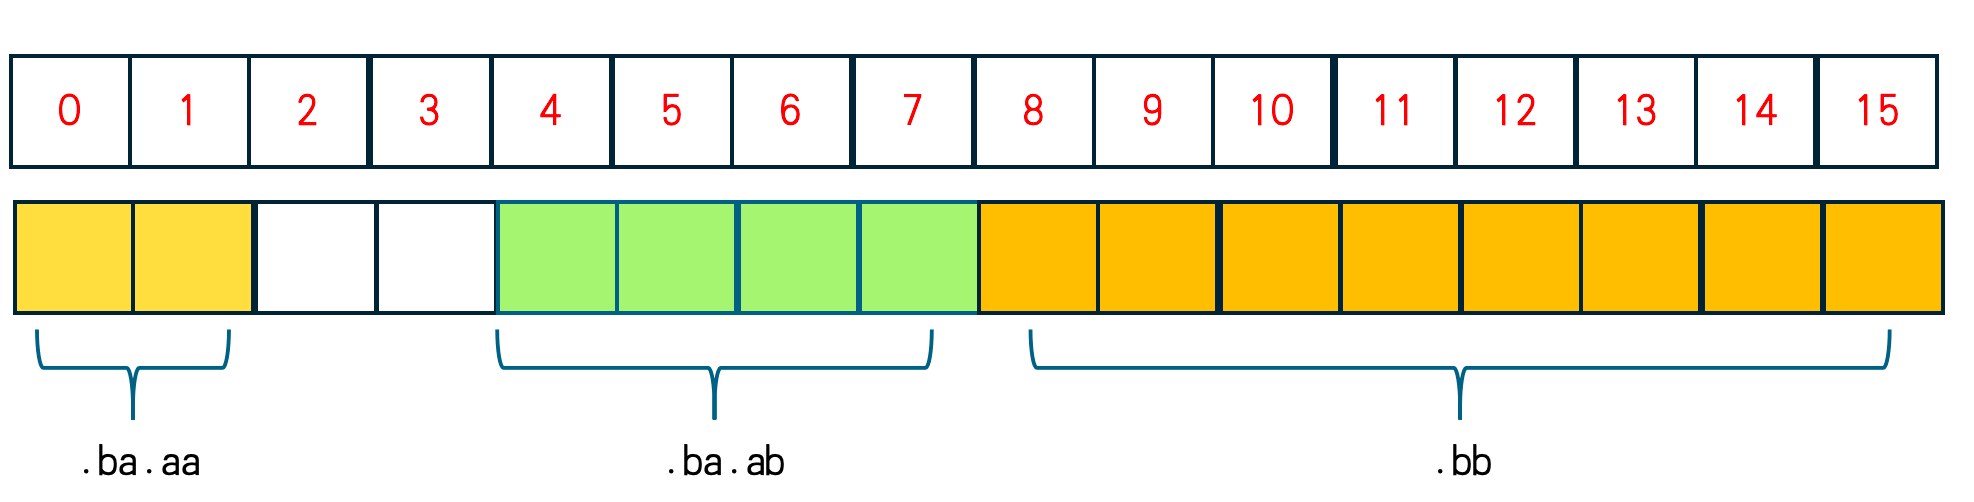
\includegraphics[width=0.7\linewidth]{23-T3/样例1.png}
        \caption{样例 1}
        \label{fig:enter-label}
    \end{figure}

    读这张图时，要特别注意：某个成员的起始地址，必须是其对齐要求的整数倍。因此即使前一个成员刚好结束，后一个成员也不一定能立刻接上。

    例如，在样例 $2$ 中，结构体内部还出现了更复杂的嵌套关系，此时不仅要看最外层结构体怎么补齐，还要看内部结构体自己的大小和对齐要求。
\begin{figure}[h]
    \centering
    
\includegraphics[width=0.7\linewidth]{23-T3/样例2.png}
    \label{fig:enter-label}
\end{figure}
\begin{figure}[h]
    \centering
    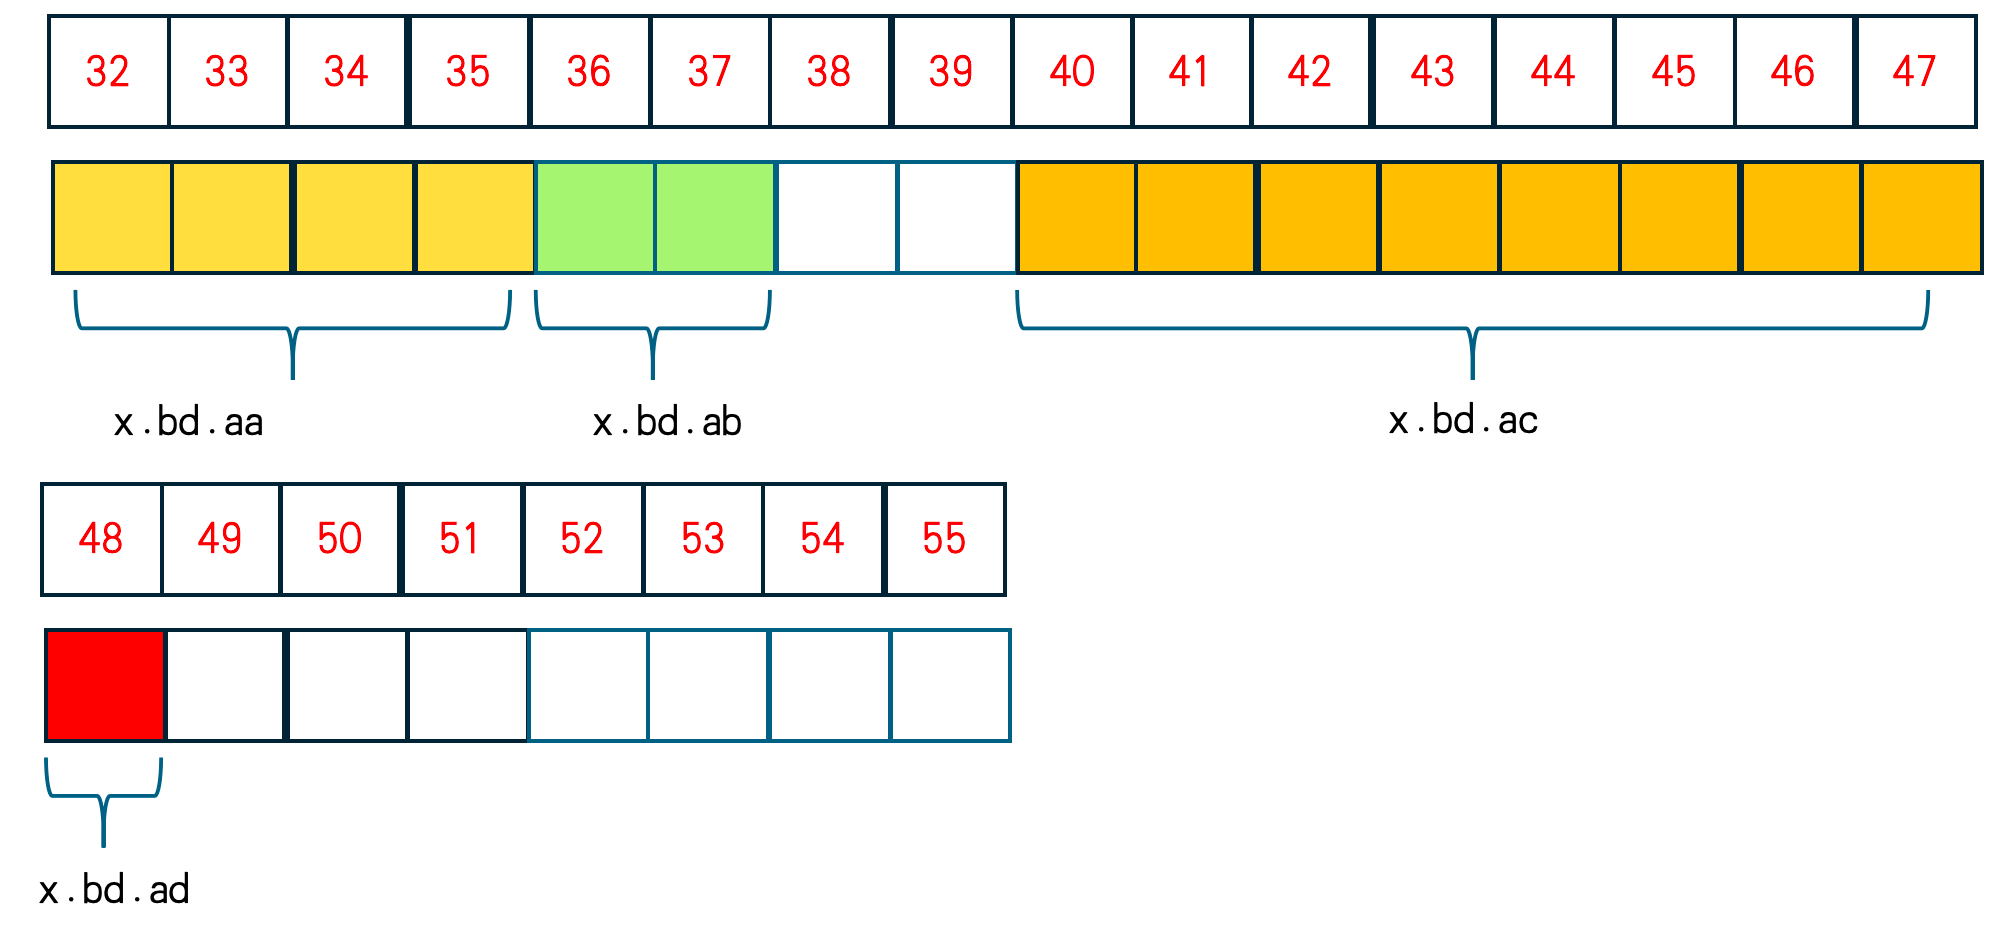
\includegraphics[width=0.7\linewidth]{23-T3/样例2.2.png}
    \caption{样例 2}
    \label{fig:enter-label}
\end{figure}

    换句话说，这道题并不是单纯模拟“成员顺序”，而是在模拟“按对齐规则摆放后的真实内存布局”。



\newpage
    \subsection{Case 1--3：只有基础类型}
        \textbf{部分分特点}：没有操作 $1$，也就是不会定义新的结构体类型，所有变量都只是基础类型。

        这时基础类型的大小和对齐要求都是固定的，因此只需要维护变量本身的信息。

        操作 $2$ 记录变量的起始位置和所占区间；操作 $3$ 直接按变量名查询；操作 $4$ 枚举所有变量区间，判断给定地址落在哪一个变量里。由于这里只有基础类型，所以不需要考虑成员偏移和嵌套访问。
        \begin{lstlisting}[style = code]
typedef long long ll;
map<string, int> mp;
vector<pair<ll,ll> > v;
map<ll, string> var_name;
map<string,int> head; // 变量的起始位置
int now_addr = 0;
int main() {
    int q; cin >> q;
    mp["byte"] = 1, mp["short"] = 2, mp["int"] = 4, mp["long"] = 8;
    while (q--) {
        int op; cin >> op;
        if (op == 1) continue;
        if (op == 2) {
            string t, name; cin >> t >> name;
            while (now_addr % mp[t] != 0) now_addr++;
            head[name] = now_addr;
            cout << now_addr << '\n';
            var_name[now_addr] = name;
            v.push_back({now_addr, now_addr + mp[t] - 1});
            now_addr += mp[t];
        }
        if (op == 3) {string s; cin >> s; cout << head[s] << '\n';}
        if (op == 4) {
            ll pos; cin >> pos;
            bool flag = false;
            for (auto x: v) {
                if (pos >= x.first && pos <= x.second) {
                    cout << var_name[x.first] << '\n';
                    flag = true; break;
                }
            }
            if (!flag) cout << "ERR\n";
        }
    }
}\end{lstlisting}
        
    
    \subsection{Case 4--13：没有结构体嵌套}
    \textbf{部分分特点}：不会出现结构体嵌套。

    这一档已经和正解很接近了。虽然没有嵌套，但我们仍然需要同时维护“结构体类型的信息”和“变量的信息”。

    \par\medskip
    \noindent\textbf{第一步：维护结构体类型}
    \par\medskip

    对于每种结构体类型，我们至少要记录四类信息：

    \begin{enumerate}[leftmargin=2em,itemsep=1pt,topsep=2pt,parsep=0pt,partopsep=0pt]
        \item 每个成员的类型和名字；
        \item 每个成员的偏移量以及长度；
        \item 结构体总大小；
        \item 结构体的对齐要求。
    \end{enumerate}

    可以用下面这个结构体统一维护：

    \begin{lstlisting}[style = code]
struct node {
    // 成员的类型与名字
    vector<pair<string, string>> member;
    // 成员偏移量与成员长度
    vector<pair<ll, ll>> offset;
    ll len, maxx;
};
map<string, node> mp;
    \end{lstlisting}

    其中 \code{member} 记录成员的类型和名字，\code{offset} 记录该成员在结构体中的起始偏移与长度，\code{len} 表示结构体总大小，\code{maxx} 表示它的对齐要求。

    \par\medskip
    \noindent\textbf{第二步：实现对齐}
    \par\medskip

    无论是在结构体内部摆放成员，还是在内存中摆放变量，都要用到同一个操作：把当前位置调整到该类型允许的下一个合法位置。

    \begin{lstlisting}[style = code]
ll Get_Offset(ll now, string name) {
    ll maxx = mp[name].maxx;
    // 向后移动到满足该类型对齐要求的位置
    while (now % maxx != 0) now++;
    return now;
}\end{lstlisting}

    有了这个函数以后，定义结构体时就可以按成员顺序依次放置：先对齐，再记录偏移，再把当前位置向后推进成员长度。全部成员放完后，还要再对整个结构体做一次补齐。

\newpage
    \begin{lstlisting}[style = code]
void Create_Struct() {
    string name; int k; cin >> name >> k;
    node now; now.len = now.maxx = 0;
    ll pos = 0;
    for (int i = 0; i < k; i++) {
        string type, member; cin >> type >> member;
        now.member.push_back({type, member});
        // 先对齐，再记录该成员在结构体中的偏移量
        pos = Get_Offset(pos, type);
        now.offset.push_back({pos, mp[type].len});
        now.maxx = max(now.maxx, mp[type].maxx);
        pos += mp[type].len;
    }
    // 先临时写回，下面才能按 name 取到这个结构体的对齐要求
    mp[name] = now;
    pos = Get_Offset(pos, name);
    now.len = pos;
    cout << now.len << " " << now.maxx << '\n';
    mp[name] = now;
}\end{lstlisting}

    基础类型可以直接预处理成四个特殊的“结构体类型”：

    \begin{lstlisting}[style = code]
mp["int"] = {{},{},4,4};
mp["long"] = {{},{},8,8};
mp["short"] = {{},{},2,2};
mp["byte"] = {{},{},1,1};\end{lstlisting}

    \par\medskip
    \noindent\textbf{第三步：维护变量信息}
    \par\medskip

    变量层面需要记录两件事：变量属于什么类型、它的起始地址是多少。除此之外，还要把变量按出现顺序存下来，方便后面由地址反查变量。

    \begin{lstlisting}[style = code]
map<string, pair<string, ll>> mp2;
vector<pair<ll, ll>> list_pos;\end{lstlisting}

    其中 \code{mp2[name]} 存的是“变量类型 + 起始地址”，而变量区间数组 \code{list\_pos} 记录的是每个变量所占的地址区间。

    定义变量的过程也很直接：先把当前空闲地址对齐到该类型要求，再输出这个位置，然后把空闲地址向后推进整个类型的大小。
\newpage
    \begin{lstlisting}[style = code]
void Create_Variable() {
    string type, name; cin >> type >> name;
    ll pos = Get_Offset(now_addr, type);
    mp2[name] = {type, pos};
    cout << pos << '\n';
    // 保存变量占用的整段区间，供地址反查使用
    list_pos.push_back({pos, pos + mp[type].len - 1});
    now_addr = pos + mp[type].len;
}\end{lstlisting}

    \par\medskip
    \noindent\textbf{第四步：处理查询}
    \par\medskip

    由于这一档数据没有结构体嵌套，所以操作 $3$ 和操作 $4$ 都会简单很多。

    对于操作 $3$，给出的访问路径至多只有一层成员，也就是形如 \code{x} 或 \code{x.y}。因此只要先按 \code{.} 拆开，再从变量起始地址出发加上对应成员偏移即可。

    \begin{lstlisting}[style = code]
ll Get_address_By_Name(string name) {
    vector<string> list;
    for (int i = 0; i < name.size(); i++) {
        if (name[i] == '.') continue;
        int j = i;
        while (j + 1 < name.size() && name[j + 1] != '.') j++;
        list.push_back(name.substr(i, j - i + 1));
        i = j;
    }
    ll st_pos = mp2[list[0]].second;
    if (list.size() == 1) return st_pos;
    string type = mp2[list[0]].first;
    for (int j = 0; j < mp[type].member.size(); j++) {
        if (mp[type].member[j].second == list[1]) {
            // 变量起始地址加上成员偏移量
            st_pos += mp[type].offset[j].first;
            break;
        }
    }
    return st_pos;
}\end{lstlisting}

\newpage
    对于操作 $4$，先判断这个地址落在哪个变量里，再在对应结构体的成员表中顺次查找，看它属于哪一个成员即可。

    \begin{lstlisting}[style = code]
string Get_Name_By_Address(ll pos) {
    node now;
    string ans;
    ll st_pos = 0;
    for (int i = 0; i < list_pos.size(); i++) {
        auto [l, r] = list_pos[i];
        if (l <= pos && pos <= r) {
            // 先找到这个地址属于哪个变量
            st_pos = l;
            break;
        }
    }
    if (st_pos == 0 && (list_pos.empty() || 
                        list_pos[0].first != 0 || pos != 0))
        return "ERR";
        
    for (auto [name, info] : mp2) {
        if (info.second == st_pos) {
            ans = name;
            now = mp[info.first];
            break;
        }
    }
    if (ans.empty()) return "ERR";
    for (int i = 0; i < now.member.size(); i++) {
        ll len = now.offset[i].second;
        if (st_pos + now.offset[i].first <= pos &&
            pos <= st_pos + now.offset[i].first + len - 1) {
            // 再判断它落在该变量的哪个成员里
            ans += "." + now.member[i].second;
            return ans;
        }
    }
    return "ERR";
}\end{lstlisting}

\par\medskip
\noindent\textbf{65 分代码框架}
\par\medskip

前面已经分别介绍过这几个函数的实现思路：\code{Get\_Offset}、\code{Create\_Struct}、\code{Create\_Variable}，以及两个查询函数 \code{Get\_address\_By\_Name} 和 \code{Get\_Name\_By\_Address}。

因此这里不再把整份代码完整重复展开，只给出主流程和需要拼接起来的函数框架。完整可编译代码可单独整理保存。

\begin{lstlisting}[style = code]
#include <bits/stdc++.h>
using namespace std;
typedef long long ll;
struct node {
    vector<pair<string, string>> member; // 成员的类型与名字
    vector<pair<ll, ll>> offset;         // 成员偏移量与成员长度
    ll len, maxx;                        // 总大小与对齐要求
};
map<string, node> mp;            // 类型名 -> 类型信息
map<string, pair<string, ll>> mp2; // 变量名 -> (类型名, 起始地址)
vector<pair<ll, ll>> list_pos;   // (变量起始地址, 结束地址)
ll now_addr;                     // 当前第一个可用地址

ll Get_Offset(ll now, string name);          // 同前文
void Create_Struct();                        // 同前文
void Create_Variable();                      // 同前文
ll Get_address_By_Name(string name);         // 同前文
string Get_Name_By_Address(ll pos);          // 同前文

void solve() {
    int q; cin >> q;
    while (q--) {
        int op; cin >> op;
        if (op == 1) Create_Struct();
        else if (op == 2) Create_Variable();
        else if (op == 3) {
            string name; cin >> name;
            cout << Get_address_By_Name(name) << '\n';
        } else {
            ll pos; cin >> pos;
            cout << Get_Name_By_Address(pos) << '\n';
        }
    }
}
int main() {
    mp["int"] = {{},{},4,4};
    mp["long"] = {{},{},8,8};
    mp["short"] = {{},{},2,2};
    mp["byte"] = {{},{},1,1};
    solve();
}\end{lstlisting}


\newpage
\subsection{满分解法}

    \textbf{部分分特点}：会出现结构体嵌套，因此访问路径可能形如 \code{x.a.b.c}。

    和上一节相比，定义结构体、定义变量、对齐规则都完全不变。真正发生变化的，只有两类查询：

    \begin{enumerate}[leftmargin=2em,itemsep=1pt,topsep=2pt,parsep=0pt,partopsep=0pt]
        \item 操作 $3$：名字查地址时，访问路径不再只是一层成员；
        \item 操作 $4$：地址查名字时，也要能够一路深入到更内层成员。
    \end{enumerate}

    \begin{keybox}{关键观察：除了第一段是变量名，后面的每一段都是成员名}
        无论是操作 $3$ 还是操作 $4$，本质上都在做同一件事：从最外层变量出发，不断进入下一层结构体。

        因此满分做法只是在上一节的基础上，把“只处理一层成员”改成了“用循环持续向下走”。
    \end{keybox}

\par\medskip
\noindent\textbf{操作 3：根据名字获取地址}
\par\medskip

    先把访问路径按 \code{.} 拆开。第一段是变量名，可以直接从 \code{mp2} 中找到它的起始地址和类型；后面的每一段都是成员名，我们只需要在当前类型的成员表中找到对应成员，把偏移量加到当前地址上，再把类型更新为该成员自己的类型即可。

        \begin{lstlisting}[style = code]
ll Get_address_By_Name(string name) {
    vector<string> list;
    for (int i = 0; i < name.size(); i++) {
        if (name[i] == '.') continue;
        int j = i;
        while (j + 1 < name.size() && name[j + 1] != '.') j++;
        list.push_back(name.substr(i, j - i + 1));
        i = j;
    }
    ll st_pos = mp2[list[0]].second;
    string type = mp2[list[0]].first;
    for (int i = 1; i < list.size(); i++) {
        for (int j = 0; j < mp[type].member.size(); j++) {
            if (mp[type].member[j].second == list[i]) {
                st_pos += mp[type].offset[j].first;
                type = mp[type].member[j].first;
                break;
            }
        }
    }
    return st_pos;
}
\end{lstlisting}

\newpage
\par\medskip
\noindent\textbf{操作 4：根据地址获取名字}
\par\medskip

    这部分的思路与操作 $3$ 是对称的。

    先像上一节一样，通过变量区间数组 \code{list\_pos} 找到这个地址属于哪个最外层变量；接下来只要不断在当前结构体的成员表中判断“地址落在哪个成员里”，如果找到了，就把这个成员名接到答案后面，再进入该成员所属的类型继续处理。

    一旦当前类型已经不是结构体，或者当前地址无法落入任何成员区间，就结束搜索。

        \begin{lstlisting}[style = code]
string Get_Name_By_Address(ll pos) {
    node now;
    string ans; ll st_pos = 0;
    for (int i = 0; i < list_pos.size(); i++) {
        auto [l, r] = list_pos[i];
        if (l <= pos && pos <= r) { st_pos = l; break; }
    }
    if (st_pos == 0 && (list_pos.empty() ||
                        list_pos[0].first != 0 || pos != 0))
        return "ERR";
    for (auto [name, info] : mp2) {
        if (info.second == st_pos) {
            ans = name; now = mp[info.first]; break;
        }
    }
    if (ans.empty()) return "ERR";
    while (!now.member.empty()) {
        bool found = false;
        for (int i = 0; i < now.member.size(); i++) {
            ll l = st_pos + now.offset[i].first;
            ll r = l + now.offset[i].second - 1;
            if (l <= pos && pos <= r) {
                ans += "." + now.member[i].second;
                st_pos = l;
                now = mp[now.member[i].first];
                found = true;
                break;
            }
        }
        if (!found) return "ERR";
    }
    return ans;
}
\end{lstlisting}
    上一节的完整代码可以直接沿用，真正需要修改的仍然只有这两个查询函数。也就是说，\code{Get\_Offset}、\code{Create\_Struct}、\code{Create\_Variable} 和 \code{solve} 都与上一节相同；两个查询函数的修改方式上文已经分别说明，这里不再重复展开。


\newpage
\section{T4. 种树} % 大标题
    
    
    \subsection{题意简析}
给定一棵包含 $n$ 个结点的树，每个结点 $i$ 有三个参数 $(a_i,b_i,c_i)$。

每天必须选择一个还没有种过、并且与当前已种结点连通的点种下去。由于第 $1$ 天必须种 $1$ 号结点，所以整个种植过程始终满足一个很重要的限制：

\begin{center}
    \textbf{每个结点都必须在父亲之后种下。}
\end{center}

如果结点 $i$ 在第 $p$ 天种下，那么到第 $D$ 天为止，它的总高度就是
\[
\sum_{x=p}^{D} \max(b_i + x c_i, 1).
\]

题目要求的是：怎样安排种植顺序，才能让所有结点都达标，并且总天数 $D$ 最小。

\subsection{从题面到模型}

这道题最难的地方，不在于“树”本身，而在于“顺序”和“截止时间”是绑在一起的。

如果把树以 $1$ 号点为根，那么“每天只能种相邻结点”就等价于：

\begin{enumerate}[leftmargin=2em,itemsep=1pt,topsep=2pt,parsep=0pt,partopsep=0pt]
    \item 每天种一个新结点；
    \item 任意结点都必须在父亲之后出现。
\end{enumerate}

于是，问题可以拆成两层：

\begin{enumerate}[leftmargin=2em,itemsep=1pt,topsep=2pt,parsep=0pt,partopsep=0pt]
    \item 先猜一个总天数 $D$；
    \item 判断是否存在一种合法的种植顺序，使得每个结点在第 $D$ 天前都能长到至少 $a_i$。
\end{enumerate}

这正是一个非常典型的“二分答案 + 可行性判定”模型。

    \begin{keybox}{关键转化：每个结点都有一个“最晚种植日”}
        在总天数固定为 $D$ 时，每个结点 $i$ 都可以反推出一个最晚种植日 $ddl_i$：

        只要在第 $ddl_i$ 天及之前种下它，它到第 $D$ 天时就一定能达标；如果再晚一天，就来不及了。

        这样一来，原题就被转化成了一个调度问题：
        \textbf{能否在“父亲先于儿子”的限制下，让每个结点都不晚于自己的截止时间被种下。}
    \end{keybox}

\newpage
\subsection{Case 1, 5--8：所有结点满足 \texorpdfstring{$c_i=0$}{ci=0}}
    \textbf{部分分特点}：所有结点都满足 $c_i = 0$。

    这时每棵树每天的增长量恒为 $b_i$，因此如果结点 $i$ 被种下后需要至少长 $t_i$ 天才能达标，那么
    \[
    t_i = \left\lceil \frac{a_i}{b_i} \right\rceil.
    \]

    由于增长速度不再随天数变化，某个结点“有多着急”只取决于它需要长多久。显然，$t_i$ 越大，就越应该尽量早种。

\par\medskip
\noindent\textbf{贪心思路}
\par\medskip

    把所有结点按 $t_i$ 从大到小排序。依次考虑这些结点：

    如果当前结点还没有被种下，就把“根到它路径上所有还没种过的结点”按顺序全部种下。

    这样做有两个好处：

    \begin{enumerate}[leftmargin=2em,itemsep=1pt,topsep=2pt,parsep=0pt,partopsep=0pt]
        \item 始终满足父亲先于儿子的限制；
        \item 越紧迫的结点越早得到可生长的时间。
    \end{enumerate}

    从交换的角度看，如果两个目标结点中一个需要更长的生长时间，那么把它对应的新增路径放到更前面，只会让答案更优，不会更差。

    \begin{keybox}{正确性说明：为什么要优先处理 $t_i$ 更大的点}
        设有两个还没处理的目标结点 $x,y$，并且 $t_x > t_y$。

        无论先处理 $x$ 还是先处理 $y$，真正新增出来的结点总数是一样的；区别只在于，这些新增结点对应的“可生长时间”是先分给谁。

        由于 $x$ 需要的生长时间更长，它比 $y$ 更紧迫。如果把 $y$ 放在前面，只会让 $x$ 的种植时间更晚，从而更容易成为答案中的瓶颈；反过来，把 $x$ 提前并不会伤害 $y$，因为 $y$ 需要的时间本来就更短。

        因此，把较大的 $t_i$ 放在前面一定不劣。再配合“每次把根到目标点的未种路径一次补齐”，就得到这一档的最优贪心策略。
    \end{keybox}

    因此，这一档的最优策略就是：\textbf{按 $t_i$ 从大到小处理目标结点，并把未出现过的根路径补上。}

\par\medskip
\noindent\textbf{时间复杂度}
\par\medskip
    排序需要 $O(n \log n)$，而每个结点至多只会被压栈、弹栈各一次，因此总复杂度为 $O(n \log n)$。

\newpage
\begin{lstlisting}[style = code]
#include <bits/stdc++.h>
using namespace std;
const int N = 1e5 + 5;
typedef long long ll;
vector<int> g[N];
ll fa[N], a[N], b[N], c[N], vis[N], t[N], idx[N];
void dfs(int u, int f) {
    fa[u] = f;
    for (int v : g[u]) if (v != f) dfs(v, u);
}
bool cmp(int x, int y) { return t[x] > t[y]; }
int main() {
    int n; cin >> n;
    for (int i = 1; i <= n; i++) {
        cin >> a[i] >> b[i] >> c[i];
        t[i] = (a[i] - 1) / b[i] + 1;
    }
    for (int i = 1; i < n; i++) {
        int u, v; cin >> u >> v;
        g[u].push_back(v), g[v].push_back(u);
    }
    dfs(1, 0);
    vis[0] = 1;
    for (int i = 1; i <= n; i++) idx[i] = i;
    sort(idx + 1, idx + n + 1, cmp);
    ll ans = 0, day = 0;
    for (int i = 1; i <= n; i++) {
        int u = idx[i];
        while (!vis[u]) {
            vis[u] = 1;
            ans = max(ans, day + t[u]);
            u = fa[u], day++;
        }
    }
    cout << ans << '\n';
}
\end{lstlisting}

\newpage
\subsection{满分解法}

    满分与上一档的差别在于：$c_i$ 不再恒为 $0$，因此某个结点能否在第 $D$ 天前达标，不仅取决于“它能长多少天”，还取决于“它具体是从哪一天开始长”的。

    但好消息是，\textbf{固定总天数 $D$ 以后，每个结点的可行种植日依然是一个前缀区间}。

    也就是说，如果结点 $i$ 在第 $p$ 天种下可以达标，那么更早的天数也一定可以；如果第 $p$ 天已经来不及了，那么更晚的天数更不可能。

\par\medskip
\noindent\textbf{第一步：二分总天数}
\par\medskip

    显然，总天数越多，所有树最终高度只会更高，因此答案具有单调性，可以二分总天数 $D$。

\par\medskip
\noindent\textbf{第二步：求每个点的最晚种植日}
\par\medskip

    对于某个固定的 $D$，我们需要计算
    \[
    \sum_{x=p}^{D} \max(b_i + x c_i, 1)
    \]
    这个值，也就是结点 $i$ 如果在第 $p$ 天种下，到第 $D$ 天时一共能长多高。

    这个式子本质上是“等差数列求和，再把小于 $1$ 的部分截成 $1$”，因此可以用一个 $O(1)$ 的函数 \code{get} 直接算出来。

    然后对每个结点二分种植日，求出最大的可行起点 $ddl_i$。如果连第 $1$ 天种下都来不及，那么当前总天数 $D$ 一定不可行。

    \begin{keybox}{例子：什么叫“最晚种植日”}
        假设某个结点满足 $a_i = 10,\ b_i = 2,\ c_i = 1$，并且我们当前二分到的总天数是 $D = 4$。

        如果它在第 $1$ 天种下，那么总高度是
        \[
        (2+1) + (2+2) + (2+3) + (2+4) = 18.
        \]

        如果它在第 $2$ 天种下，那么总高度是
        \[
        (2+2) + (2+3) + (2+4) = 15.
        \]

        如果它在第 $3$ 天种下，那么总高度是
        \[
        (2+3) + (2+4) = 11.
        \]

        如果它在第 $4$ 天种下，那么总高度是
        \[
        2+4 = 6.
        \]

        因此，第 $1,2,3$ 天都还来得及，第 $4$ 天已经来不及，于是这个点的最晚种植日就是 $ddl_i = 3$。

        注意这里的可行天数一定形成一个前缀：能在第 $3$ 天种，就一定也能在第 $1,2$ 天种；也正因为这个单调性，我们才可以对种植日做二分。
    \end{keybox}

    \begin{keybox}{判定问题的本质}
        固定总天数 $D$ 后，我们得到每个结点的最晚种植日 $ddl_i$。

        接下来要做的，就是判断能否安排一个合法顺序，使得每个结点都在第 $ddl_i$ 天之前被种下。

        这和上一档其实是同一个贪心框架，只不过“紧迫程度”从原来的 $t_i$，变成了现在的截止时间 $ddl_i$。
    \end{keybox}

\par\medskip
\noindent\textbf{第三步：按截止时间从小到大贪心}
\par\medskip

    把所有结点按 $ddl_i$ 从小到大排序，也就是先处理最着急的点。

    依次考虑这些点：如果它还没有被种下，就把它到最近已种祖先之间的整条路径全部补上。

    设当前一共已经种了 \code{res} 个点。如果在处理某个结点时出现 \code{res > ddl\_i}，说明它最晚应该在第 $ddl_i$ 天种下，但我们已经来不及了，因此当前 $D$ 不可行。

    否则，这个 $D$ 就可以完成全部种植。

\par\medskip
\noindent\textbf{时间复杂度}
\par\medskip
    单次 \code{check} 需要 $O(n \log D + n \log n)$，前一项来自对每个点二分最晚种植日，后一项来自排序。再套上一层答案二分，总复杂度为
    \[
    O\bigl(\log D \cdot (n \log D + n \log n)\bigr).
    \]

\newpage
\begin{lstlisting}[style = code]
#include <bits/stdc++.h>
using namespace std;
typedef long long ll;
typedef __int128 i128;
const int N = 1e5 + 5;
vector<int> g[N];
ll a[N], b[N], c[N];
int fa[N], vis[N], n;
pair<int, int> ddl[N]; // (最晚种植日, 结点编号)
void dfs(int u, int f) {
    fa[u] = f;
    for (int v : g[u]) if (v != f) dfs(v, u);
}
// 这是一个首项为 b + c * l，末项为 b + c * r，项数为 r - l + 1 的等差数列求和。
i128 calc_sum(ll b, ll c, ll l, ll r) {
    i128 first = (i128)b + (i128)c * l, last = (i128)b + (i128)c * r;
    i128 cnt = r - l + 1;
    return (first + last) * cnt / 2;
}
// 计算从第 l 天到第 r 天，树的总生长高度。
i128 get(ll b, ll c, ll l, ll r) {
    if (c >= 0) return calc_sum(b, c, l, r);
    ll k = -c;
    // 最后一天满足 b + c * x >= 1。
    ll last = (b - 1) / k;
    // [l, r] 中每天的增长量都已经变成 1。
    if (last < l) return r - l + 1;
    // [l, r] 中每天的增长量都还大于等于 1。
    if (r <= last) return calc_sum(b, c, l, r);
    // [l, last] 按等差数列计算，[last + 1, r] 每天增长量都是 1。
    return calc_sum(b, c, l, last) + (r - last);
}
int Get_Last_Day(int id, int day_limit) {
    if (get(b[id], c[id], 1, day_limit) < a[id]) return 0;
    int l = 1, r = day_limit + 1;
    while (l < r) {
        int mid = (l + r) >> 1;
        if (get(b[id], c[id], mid, day_limit) >= a[id]) l = mid + 1;
        else r = mid;
    }
    return l - 1;
}

bool check(int day_limit) {
    for (int i = 1; i <= n; i++) vis[i] = 0;
    vis[0] = 1;
    for (int i = 1; i <= n; i++) {
        int last_day = Get_Last_Day(i, day_limit);
        if (!last_day) return false;
        ddl[i] = {last_day, i};
    }
    sort(ddl + 1, ddl + n + 1); // 按最晚种植日从小到大排序
    int res = 0;
    for (int i = 1; i <= n; i++) {
        int u = ddl[i].second;
        int cnt = 0;
        while (!vis[u]) {
            vis[u] = 1;
            u = fa[u], cnt++;
        }
        res += cnt;
        if (res > ddl[i].first) return false;
    }
    return true;
}

int main() {
    cin >> n;
    for (int i = 1; i <= n; i++) cin >> a[i] >> b[i] >> c[i];
    for (int i = 1; i < n; i++) {
        int u, v;
        cin >> u >> v;
        g[u].push_back(v);
        g[v].push_back(u);
    }
    dfs(1, 0);
    int l = n, r = 1000000000;
    while (l < r) {
        int mid = (l + r) >> 1;
        if (check(mid)) r = mid;
        else l = mid + 1;
    }
    cout << l << '\n';
}\end{lstlisting}

\chapter{2024 CSP-S复赛解析}
\newpage

    \section{T1. 决斗} % 大标题
    
    
    \subsection{题意简析}

    有 $n$ 个怪兽，第 $i$ 个怪兽的攻击力为 $r_i$。每一轮可以选一只怪兽攻击另一只怪兽；若攻击者的攻击力严格更大，则被攻击者被击败并永久退出游戏，否则这一轮不会产生任何影响。

    每只仍然留在场上的怪兽最终都必须发起过一次攻击。问如何安排攻击过程，才能使最后剩下的怪兽数量最少。

    
    \subsection{从题面到模型}

    一次\textbf{有效攻击}会让场上的怪兽数量减少 $1$，无效攻击则不会改变答案。因此，最少剩下多少怪兽，等价于\textbf{最多能安排多少次有效攻击}。

    于是问题可以转化为：尽量构造更多满足“攻击者攻击力严格大于被攻击者攻击力”的配对。每成功配出一对，就对应一次有效攻击，答案也会减少 $1$。

    
    \subsection{满分解法：排序 + 双指针贪心}

    先将所有攻击力从小到大排序，记为 $a_1\le a_2\le \cdots \le a_n$。

    我们用指针 $l$ 表示“当前最弱、且还没有被击败的怪兽”所在位置。随后按攻击力从小到大枚举每一只怪兽作为攻击者：

    \begin{itemize}[leftmargin=2em,itemsep=1pt,topsep=2pt,parsep=0pt,partopsep=0pt]
        \item 如果当前怪兽的攻击力不超过 $a_l$，那么它连当前最弱的存活怪兽都打不过，这次攻击不可能产生贡献，只能跳过。
        \item 如果当前怪兽的攻击力大于 $a_l$，那么就让它击败这只最弱的存活怪兽，并将 $l$ 右移一位。
    \end{itemize}

    \begin{keybox}{关键观察：能击败时，优先击败当前最弱的存活怪兽一定不劣}
    如果当前怪兽能够击败某只存活怪兽，那么它也一定能够击败其中最弱的那只。此时优先消灭最弱者，不会减少后面怪兽的选择空间，反而能把更强的怪兽留给后续更难配对的位置。因此，贪心地“能杀就杀当前最弱者”始终最优。
    \end{keybox}

    这种枚举顺序还有一个好处：攻击力较小的怪兽更难完成有效攻击，因此应当优先让它们尝试出手；如果连它都能完成一次击败，那么后面更强的怪兽只会更容易继续完成配对。

    \begin{examplebox}{例子：\texorpdfstring{$1,2,2,3,4$}{1,2,2,3,4}}
    排序后序列仍为 $1,2,2,3,4$。一开始 $l=1$，指向攻击力为 $1$ 的怪兽。

    枚举到第一只攻击力为 $2$ 的怪兽时，由于 $2>1$，它可以击败这只攻击力为 $1$ 的怪兽，于是 $l$ 右移。

    接着枚举到第二只攻击力为 $2$ 的怪兽时，此时 $l$ 指向另一只攻击力为 $2$ 的怪兽，而 $2\not>2$，所以这次攻击无法产生贡献。

    再往后，攻击力为 $3$ 和 $4$ 的怪兽都可以各自再击败一只当前最弱的存活怪兽，最后总共完成 $3$ 次有效攻击，因此答案为 $5-3=2$。
    \end{examplebox}

    排序的时间复杂度为 $O(n\log n)$，双指针扫描的时间复杂度为 $O(n)$，因此总时间复杂度为 $O(n\log n)$，空间复杂度为 $O(1)$（不计排序使用的额外空间）。
    
    \begin{lstlisting}[style = code]
#include<bits/stdc++.h>
using namespace std;

const int N = 1e5 + 5;
int a[N];

int main() {
    int n;
    cin >> n;
    for (int i = 1; i <= n; i++) cin >> a[i];

    sort(a + 1, a + n + 1);
    int l = 1;
    for (int i = 1; i <= n; i++) {
        if (a[i] > a[l]) l++;
    }

    cout << n - l + 1 << '\n';
    return 0;
}
    \end{lstlisting}
    
    
    \newpage
    
    
    
    \section{T2. 超速检测}


    \subsection{题意简析}
    
    有一条长度为 $L$ 的道路，$n$ 辆车会在不同位置驶入道路，并以给定初速度和加速度向前行驶。道路上有 $m$ 个测速仪，每个测速仪可以选择开启或关闭。

    当一辆车经过某个开启的测速仪时，若它在该位置的瞬时速度严格大于限速 $V$，那么这辆车会被判定为超速。

    题目要求回答两件事：第一，在所有测速仪都开启时，有多少辆车会被判定为超速；第二，在不漏掉这些超速车辆的前提下，最多可以关闭多少个测速仪。

    
    \subsection{从题面到模型}

    设某辆车在位置 $x$ 处时，距离它驶入道路的位置前进了 $x-d_i$。根据题目给出的公式，它在该位置的速度满足
    $v^2=v_i^2+2a_i(x-d_i)$。

    因为我们只关心它是否超速，所以没有必要真的求出速度，只需比较
    $v_i^2+2a_i(x-d_i)$ 与 $V^2$ 的大小关系即可。这样可以完全避免浮点误差。

    更关键的是：对固定的一辆车来说，使它超速的位置一定构成一个\textbf{连续区间}。

    \begin{itemize}[leftmargin=2em,itemsep=1pt,topsep=2pt,parsep=0pt,partopsep=0pt]
        \item 当 $a_i=0$ 时，速度恒定，要么整段都不超速，要么从驶入开始整段都超速。
        \item 当 $a_i>0$ 时，速度单调增大，超速位置一定是一个后缀区间。
        \item 当 $a_i<0$ 时，速度单调减小，超速位置一定是一个前缀区间。
    \end{itemize}

    因此，每辆会被检测到超速的车，都对应着一个“哪些测速仪可以拍到它超速”的连续区间。

    \subsection{Case 1--2：直接暴力}

    \textbf{部分分特点}：$n,m\le 20$。

    第一问可以直接枚举每一辆车和每一个测速仪，用上面的速度平方公式判断该车在这个测速仪处是否超速。

    第二问如果继续暴力，可以枚举每个测速仪的开关状态，检查是否漏掉了原本会被判超速的车辆。

    这样第一问复杂度为 $O(nm)$，第二问复杂度为 $O(2^m\cdot nm)$，只能通过最前面的几个测试点。

    下面给出这一部分的完整暴力代码。这里直接使用 DFS 枚举每个测速仪“开/关”两种选择。

    \begin{lstlisting}[style = code]
#include <bits/stdc++.h>
using namespace std;
typedef long long ll;
const int N = 25;
int n, m, L, V;
int d[N], v[N], a[N], p[N];
// 第 i 个摄像头开或者不开
bool choose[N];
// 第 i 辆车是否超速
bool all_caught[N];
int ans1, best_keep;

// 判断在第某个摄像头处，车子是否超速
bool over_speed(int car, int cam) {
    if (p[cam] < d[car]) return false;
    ll dist = p[cam] - d[car];
    ll now = 1LL * v[car] * v[car] + 2LL * a[car] * dist;
    if (now < 0) return false; // 车在到达测速仪前已经停下
    return now > 1LL * V * V;
}
bool caught_with_now(int car) {
    for (int j = 1; j <= m; j++) 
        if (choose[j] && over_speed(car, j)) return true;
    return false;
}
void dfs(int now) {
    if (now > m) {
        int keep = 0;
        for (int i = 1; i <= m; i++) keep += choose[i];
        for (int i = 1; i <= n; i++) 
            if (all_caught[i] && !caught_with_now(i)) return;
        best_keep = min(best_keep, keep);
        return;
    }
    choose[now] = false, dfs(now + 1);
    choose[now] = true, dfs(now + 1);
}
void solve() {
    cin >> n >> m >> L >> V;
    for (int i = 1; i <= n; i++) cin >> d[i] >> v[i] >> a[i];
    for (int i = 1; i <= m; i++) cin >> p[i];
    ans1 = 0;
    for (int i = 1; i <= n; i++) {
        all_caught[i] = false;
        for (int j = 1; j <= m; j++) 
            if (over_speed(i, j)) all_caught[i] = true;
        ans1 += all_caught[i];
    }
    best_keep = m;
    dfs(1);
    cout << ans1 << " " << m - best_keep << '\n';
}
int main() { int T;cin >> T;while (T--) solve();}
\end{lstlisting}


    \subsection{特殊性质 A、B、C}

    \textbf{部分分特点}：特殊性质 A 保证 $a_i=0$，特殊性质 B 保证 $a_i>0$，特殊性质 C 保证 $a_i<0$，且车辆不会在道路北端驶出。

    这三类特殊性质的价值在于，它们分别对应了三种最典型的超速区间形态。把这三种情况分别看清，满分做法的区间建模就会自然很多。

    \par\medskip
    \noindent\textbf{特殊性质 A：$a_i=0$}
    \par\medskip

    此时速度恒定。若 $v_i\le V$，整段都不超速；若 $v_i>V$，那么从驶入位置开始一直到离开道路，这辆车始终超速。

    因此，只要驶入位置之后存在测速仪，这辆车就一定会被拍到；而在第二问中，只要保留最后一个测速仪，就能拍到所有会被检测到超速的车辆。

    对应代码非常直接：

    \begin{lstlisting}[style = code]
int x = lower_bound(p + 1, p + m + 1, d[i]) - p;
if (x <= m && v[i] > V) seg[++tot] = {x, m};\end{lstlisting}

    \par\medskip
    \noindent\textbf{特殊性质 B：$a_i>0$}
    \par\medskip

    此时速度单调增大，所以超速位置一定是一个后缀区间。也就是说，一旦某辆车在某个测速仪处超速，那么它之后经过的测速仪也都会拍到它超速。

    因此和特殊性质 A 一样，只要一辆车会被拍到超速，那么最后一个测速仪一定也能拍到它。第二问仍然只需保留最后一个测速仪。

    如果希望把“第一个会超速的测速仪”也求出来，可以直接二分：

    \begin{lstlisting}[style = code]
if (x <= m && over_speed(i, m)) {
    int l = x, r = m;
    while (l < r) {
        int mid = l + r >> 1;
        if (over_speed(i, mid)) r = mid;
        else l = mid + 1;
    }
    seg[++tot] = {l, m};
}\end{lstlisting}

    \par\medskip
    \noindent\textbf{特殊性质 C：$a_i<0$}
    \par\medskip

    此时速度单调减小，所以超速位置一定是一个前缀区间。如果一辆车初始时没有超速，那么后面更不可能超速；如果它一开始超速，那么只会在前面一段位置内超速，之后速度降下来就不会再被拍到。

    这说明真正的难点在于：不同车辆对应的“可拍到超速的测速仪区间”不再都包含最后一个测速仪了，因此第二问不能再用一个简单特判解决。

    这时要找的是“最后一个仍然超速的测速仪”：
\newpage
    \begin{lstlisting}[style = code]
if (x <= m && over_speed(i, x)) {
    int l = x, r = m;
    while (l < r) {
        int mid = l + r + 1 >> 1;
        if (over_speed(i, mid)) l = mid;
        else r = mid - 1;
    }
    seg[++tot] = {x, l};
}\end{lstlisting}

    \subsection{满分解法：二分求区间 + 区间选点覆盖}

    前面的瓶颈在于：虽然我们已经知道一辆车的超速位置是一个连续区间，但如果还要逐个测速仪去判断它能否拍到这辆车，代价仍然太高。

    由于测速仪位置 $p_1<p_2<\cdots<p_m$ 已经有序，我们可以直接把“位置区间”转成“测速仪编号区间”。

    \begin{keybox}{关键建模：第二问是最少选点覆盖所有区间}
    对于每一辆会被拍到超速的车，记它会被哪些测速仪拍到超速为一个编号区间。第二问就变成：从所有测速仪中选尽量少的点，使得每个区间里至少选中一个点。最后最多关闭的数量就是 $m-$最少需要保留的测速仪数量。
    \end{keybox}

    设 $x$ 是驶入位置右侧的第一个测速仪编号，即 $p_x\ge d_i$。如果 $x>m$，说明这辆车驶入之后一个测速仪都遇不到，可以直接跳过。

    接下来分三类讨论：

    \begin{enumerate}[leftmargin=2em,itemsep=1pt,topsep=2pt,parsep=0pt,partopsep=0pt]
        \item $a_i=0$：若 $v_i\le V$，它永远不超速；否则所有编号在 $[x,m]$ 的测速仪都能拍到它。
        \item $a_i>0$：超速测速仪构成一个后缀。先判断最后一个测速仪处是否已经超速；若否则这辆车不会被拍到，若是则二分第一个超速的测速仪编号，得到区间 $[l,m]$。
        \item $a_i<0$：超速测速仪构成一个前缀。先判断第一个会遇到的测速仪处是否已经超速；若否则这辆车不会被拍到，若是则二分最后一个仍然超速的测速仪编号，得到区间 $[x,r]$。
    \end{enumerate}

    这样每辆车只需二分一次，就能直接得到它对应的测速仪编号区间。第一问的答案就是这类区间的个数；第二问则转化成这些区间上的最少选点问题。

    \begin{keybox}{关键观察：按右端点排序后，贪心选最右点最优}
    当我们处理到某个区间时，如果当前已选的最后一个测速仪不在这个区间里，就必须新增一个测速仪。此时选择该区间最右端的测速仪一定不劣，因为它在覆盖当前区间的同时，还最有希望继续覆盖后面的区间。
    \end{keybox}

    \begin{examplebox}{例子：为什么要选区间右端点}
    假设三辆会被拍到超速的车，对应的测速仪编号区间分别是 $[2,4]$、$[3,5]$、$[5,6]$。

    先处理右端点最小的区间 $[2,4]$。如果新增一个测速仪，那么选编号 $4$ 一定优于选编号 $2$ 或 $3$，因为它不仅覆盖当前区间，还顺便覆盖了后面的区间 $[3,5]$。

    接下来只剩区间 $[5,6]$ 没有被覆盖，再选编号 $6$ 即可。于是总共只需保留两个测速仪。
    \end{examplebox}

    对每辆车，我们先用 \code{lower\_bound} 找到驶入后遇到的第一个测速仪，再做一次二分，因此求出全部区间的复杂度为 $O(n\log m)$。随后对所有区间排序并做贪心，复杂度为 $O(n\log n)$。因此总时间复杂度为 $O(n\log m+n\log n)$，空间复杂度为 $O(n+m)$。

    \begin{lstlisting}[style = code]
#include<bits/stdc++.h>
using namespace std;
typedef long long ll;
const int N = 100000 + 5;
struct Interval {
    int l, r;
} seg[N];
int d[N], v[N], a[N], p[N];
int V;
bool cmp(Interval x, Interval y) {
    if (x.r != y.r) return x.r < y.r;
    return x.l < y.l;
}
bool over_speed(int id, int pos) {
    ll dist = p[pos] - d[id];
    ll now = 1LL * v[id] * v[id] + 2LL * a[id] * dist;
    return now > 1LL * V * V;
}
int first_camera(int id, int m) {
    return lower_bound(p + 1, p + m + 1, d[id]) - p;
}

void build_interval(int id, int m, int &tot) {
    int x = first_camera(id, m);
    if (x > m) return;
    if (a[id] == 0) {
        if (v[id] > V) seg[++tot] = {x, m};
        return;
    }
    if (a[id] > 0) {
        if (!over_speed(id, m)) return;
        int l = x, r = m;
        while (l < r) {
            int mid = l + r >> 1;
            if (over_speed(id, mid)) r = mid;
            else l = mid + 1;
        }
        seg[++tot] = {l, m};
        return;
    }
    if (!over_speed(id, x)) return;
    int l = x, r = m;
    while (l < r) {
        int mid = l + r + 1 >> 1;
        if (over_speed(id, mid)) l = mid;
        else r = mid - 1;
    }
    seg[++tot] = {x, l};
}
int cover_intervals(int tot) {
    sort(seg + 1, seg + tot + 1, cmp);
    int keep = 0, last = 0;
    for (int i = 1; i <= tot; i++) {
        if (seg[i].l <= last && last <= seg[i].r) continue;
        last = seg[i].r;
        keep++;
    }
    return keep;
}
void solve() {
    int n, m, L;
    cin >> n >> m >> L >> V;
    for (int i = 1; i <= n; i++) cin >> d[i] >> v[i] >> a[i];
    for (int i = 1; i <= m; i++) cin >> p[i];

    int tot = 0;
    for (int i = 1; i <= n; i++) build_interval(i, m, tot);
    int keep = cover_intervals(tot);
    cout << tot << ' ' << m - keep << '\n';
}
int main() {int T;cin >> T;while (T--) solve();}\end{lstlisting}
    \newpage
    \section{T3. 染色} % 大标题
    
    
    \subsection{题意简析}

    
    给定 $n$ 个数字 $a_i$ ，你需要将每个数字涂成红色或蓝色，使数组的得分最大。
    对于每个数字 $a_i$，如果上一个与当前数字同色的数字 $a_j$ 与当前数字的值相同，则可以获得该数字的分数。即若对于任意两个整数$i, j(i < j)$， $col_i = col_j$ 且 $a_i = a_j$ 且 $col_k \neq col_i (i < k < j) $，则数组可以获得 $a_i$分。

    \subsection{从题面到模型}

    一个位置能否得分，只取决于一件事：\textbf{它在同色序列中的上一个元素是谁}。

    如果把所有红色位置单独抽出来、把所有蓝色位置也单独抽出来，那么题目的得分规则就变成了：

    \begin{itemize}[leftmargin=2em,itemsep=1pt,topsep=2pt,parsep=0pt,partopsep=0pt]
        \item 在红色序列中，若相邻两个数相等，就贡献这个数的值；
        \item 在蓝色序列中，同样如此。
    \end{itemize}

    因此整道题的关键不是“当前位置染成什么颜色”，而是“染完以后，这个颜色的上一个数是多少”。后面的动态规划和满分优化，都是围绕这条信息展开的。

    
    \subsection{Case 1--4：枚举每个位置的颜色}

        \textbf{部分分特点}：$n\leq 15, A_i\leq 15$。

        数字个数很小，可以直接枚举每个位置染成红色还是蓝色。

        当所有位置的颜色都确定以后，按顺序扫一遍数组，分别维护红色和蓝色最近出现的数字，就能直接算出当前方案的得分。因此可以用 DFS 枚举所有 $2^n$ 种染色方案，再取最大值。

        时间复杂度为 $O(n \cdot 2^n)$。

        \newpage
        \begin{lstlisting}[style = code]
#include<bits/stdc++.h> 
using namespace std;
int a[100005], col[100005];
int n;
int ans = 0;
void qidong() {
    int sum = 0;
    // lst0: 上一个颜色为0的数字
    // lst1: 上一个颜色为1的数字
    int lst0 = 0, lst1 = 0;
    for (int i = 1; i <= n; i++) {
        if (col[i] == 0) {
            if (a[i] == lst0) sum += a[i];
            lst0 = a[i];
        }
        if (col[i] == 1) {
            if (a[i] == lst1) sum += a[i];
            lst1 = a[i];
        }
    }
    ans = max(ans, sum);
}
void dfs(int now) {
    if (now == n + 1) {
        qidong();
        return ;
    }
    col[now] = 0, dfs(now + 1);
    col[now] = 1, dfs(now + 1);
}
void solve() {
    cin >> n;
    for (int i = 1; i <= n; i++) cin >> a[i];
    ans = 0;
    dfs(1);
    cout << ans << endl;
}
int main() {
    int T = 1; cin >> T;
    while (T--) solve();
}\end{lstlisting}
        
    \subsection{Case 5--10：记录另一种颜色的最后一个数字}

    \textbf{部分分特点}：$n\leq 2000, A_i\leq 2000$。

    对于这一部分，数据范围已经不允许继续枚举所有染色方案，需要改用动态规划。

    一个容易想到但不够用的状态是：只记录前 $i$ 个数字中最后一个数字的颜色。问题在于，当前位置能否得分，不只取决于上一个位置的颜色，还取决于\textbf{同色序列中上一个数字的值}。

    因此需要把状态设计成：
    \[
    dp_{i,j,k}
    \]
    表示前 $i$ 个数字已经处理完毕，当前最后一个数字的颜色为 $k$，而另一种颜色最近出现的数字值为 $j$ 时的最大得分。这里约定红色为 $0$，蓝色为 $1$。

    例如在以下样例中
    
    4
    
    \textcolor{red}{2} \textcolor{blue}{5} \textcolor{blue}{5}  2 

    $dp_{3,2,1} = 3$ 表示前3个数字，最后一个数字为蓝色，且上一个红色数字为2时，可以获得的最大得分是5。
    此时我们有 $dp_{4,5,0} = dp_{3,2,1} + 2 = 7$ 。原因是我们发现当前 $3$ 个数字的最后一个红色数字为 $a_4$ 的时候，可以通过将 $a_4$ 涂成红色得到对应的分数。

    于是可以写出下面几类转移：

    1. 如果当前第 $i$ 个数字染成红色，且上一个数字也为红色时，前 i - 1 个数字的最后一个蓝色数字为 $j$。此时上一个蓝色数字没有发生变化，仍然为 $j$。仅当 $a_i = a_{i - 1}$ 时，可以额外得到 $a_i$ 分。

    因此有：$dp_{i, j, 0} = dp_{i - 1, j, 0} + a_i[a_i = a_{i - 1}]$。($a_i[a_i=a_{i-1}]$表示若满足条件 $a_i = a_{i - 1}$ 则为 $a_i$ ，否则为0，下同。

    2. 如果当前第 $i$ 个数字染成红色，且上一个数字也为蓝色时，前 i - 1 个数字的最后一个红色数字为 $j$。对于第 $i$ 个数字来说，前 $i$ 个数字的上一个蓝色数字将变为 $a_{i - 1}$。此时仅当 $a_i = j$ 时可以得分。

    因此有 $dp_{i, a_{i - 1}, 0} = dp_{i - 1, j, 1} + a_i[a_i =j]$。

    3. 同理可得当第 $i$ 个数字为蓝色时的两个转移方程：

    $dp_{i,j,1} = dp_{i-1,j,1} + a_i[a_i = a_{i-1}]$

    $dp_{i,a_{i-1},1} = dp_{i-1,j,0} + a_i[a_i=j]$

    最后答案为
    \[
    \max \{ dp_{n,j,k} \mid 1 \leq j \leq n,\ k \in \{0,1\} \}.
    \]

    这样时间复杂度和空间复杂度都为 $O(nA)$。

    另外，这个子任务也可以用 $O(n^2)$ 的时间复杂度解决，只需要把 $dp_{i,j,k}$ 中 $j$ 的含义由“上一个与第 $i$ 个数字颜色不同的数字的值”改成“上一个与第 $i$ 个数字颜色不同的位置编号”即可。
    

    \newpage
        \begin{lstlisting}[style = code]
#include <bits/stdc++.h>
using namespace std;
int dp[2005][2005][2], a[2005]; 

void solve() {
    int n;
    cin >> n;
    for (int i = 0; i <= n; i++) {
        for (int j = 0; j <= 2000; j++) {
            dp[i][j][0] = dp[i][j][1] = -1e9;
        }
    }
    dp[1][0][0] = dp[1][0][1] = 0;
    
    for (int i = 1; i <= n; i++) cin >> a[i];
    for (int i = 2; i <= n; i++){
        for (int j = 0; j <= 2000; j++) {
            dp[i][j][0] = max(dp[i][j][0], 
                          dp[i - 1][j][0] + (a[i] == a[i - 1] ? a[i] : 0));
            dp[i][a[i - 1]][0] = max(dp[i][a[i - 1]][0], 
                                 dp[i - 1][j][1] + (a[i] == j ? a[i] : 0));
            dp[i][j][1] = max(dp[i][j][1], 
                          dp[i - 1][j][1] + (a[i] == a[i - 1] ? a[i] : 0));
            dp[i][a[i - 1]][1] = max(dp[i][a[i - 1]][1], 
                                 dp[i - 1][j][0] + (a[i] == j ? a[i] : 0));
        }
    }
    int ans = 0;
    for (int j = 0; j <= 2000; j++){
        ans = max(ans, max(dp[n][j][0], dp[n][j][1]));
    }
    cout << ans << endl;
}
int main() {
    int T; cin >> T;
    while (T--) solve();
}
\end{lstlisting}
\newpage

    \subsection{Case 13--15：沿用 $O(nA)$，按值域选实现}

    \textbf{部分分特点}：$n\leq 2\times 10^5, A_i\leq 10$。

    这一部分中，虽然 $n$ 很大，但值域很小，因此上一节的 $O(nA)$ 做法仍然可以通过。真正的问题不在时间，而在空间：如果仍然直接开 $200000\times 2000$ 的数组，会直接 MLE。

    因此可以按值域选择实现方式：当值域很小时，用小数组存状态；否则沿用上一节的大值域写法。

    \begin{lstlisting}[style = code]
int main() {
    int T;
    cin >> T;
    while (T--) {
        cin >> n;
        for (int i = 1; i <= n; i++) cin >> a[i];
        int mx1 = 0;
        for (int  i= 1; i <= n; i++) {
            mx1 = max(mx1, a[i]);
        }
        if (mx1 > 10) solve(); // 使用dp[2005][2005];
        else solve2();  // 使用dp2[200005][2]
    }
}
    \end{lstlisting}

\subsection{满分解法：从值域状态转到上一个相同位置}

    现在已经有了一个 $O(nA)$ 的算法。满分数据下，继续按值域枚举状态已经不够，需要把“值域”这一维去掉。

    回到得分条件本身：当前位置 $i$ 只有在它与某个更早的位置 $j$ 数值相同、颜色相同，并且中间所有位置都染成另一种颜色时，才会获得 $a_i$ 分。因此，真正关键的不是“这个值是多少”，而是“上一个与它相同的位置在哪里”。

    设 $lst_i$ 表示与 $a_i$ 相同的上一个位置。若想让 $a_i$ 贡献分数，那么最自然的选择就是让它与 $lst_i$ 同色，并让区间 $(lst_i,i)$ 中的数字都放到另一种颜色上。于是转移就只需要围绕 $lst_i$ 展开，而不必再枚举整个值域。

    这样一来，中间那一段“全部染成另一种颜色”所产生的贡献，就会变成一段连续区间贡献。由于这段区间里相邻同值产生的贡献可以预处理前缀和，所以这一部分可以直接 $O(1)$ 求出。

    真正难处理的，是连接点附近那一部分贡献。因为即使决定了 $a_i$ 与 $lst_i$ 同色，$lst_i$ 左边那一位的颜色仍然可能不同，从而影响转移来源。
    
    为了绕开这一点，可以把状态改写成从 $lst_i+1$ 转移，也就是把“连接点附近那一部分贡献”提前折进状态里。这样转移时只需要补上中间区间的贡献和当前位置的 $a_i$ 即可。

    这正是代码里
    \[
    dp[lst_i+1][j^1] + \bigl(pre[i-1]-pre[lst_i+1]\bigr) + a_i
    \]
    这类转移的来源。

    如果用 \code{map} 维护每个值上一次出现的位置，那么求出所有 $lst_i$ 的复杂度是 $O(n\log n)$；其余转移都是线性的。因此这份写法的总时间复杂度为 $O(n\log n)$，空间复杂度为 $O(n)$。

\begin{lstlisting}[style = code]
ll n, a[maxn], pre[maxn], dp[maxn][2];
ll lst[maxn]; // 第i个数字的上一个同数字的元素位置
void solve() {
    cin >> n;
    for (int i = 1; i <= n; i++) {
        cin >> a[i], pre[i] = 0, lst[i] = -1, dp[i][0] = dp[i][1] = 0;
    }
    for (int i = 2; i <= n; i++) {
        pre[i] = pre[i - 1] + a[i] * (a[i] == a[i - 1]);
    }
    map<int,int> mp;
    for (int i = 1; i <= n; i++) {
        lst[i] = mp[a[i]];
        mp[a[i]] = i;
    }
    dp[1][0] = dp[1][1] = 0;
    for (int i = 2; i <= n; i++) {
        for (int j = 0; j < 2; j++) {
            // a[i] 不贡献分数
            dp[i][j] = max(dp[i - 1][j ^ 1], dp[i - 1][j]);
            // a[i] 贡献分数  i与lst[i]均为col色
            if (!lst[i]) continue ; // 前面没有同色
            if (lst[i] == i - 1) { // 上一个数字就与当前同色
                dp[i][j] = max(dp[i][j], dp[i - 1][j] + a[i]);
                continue ;
            }
            // [lst[i] + 1, i - 1]均为蓝色，[lst[i] + 2, i - 1]的所有元素若与前一个相同则产生贡献
            // pre[i - 1] - pre[lst[i] + 2 - 1] 为区间贡献
            ll other_col = pre[i - 1] - pre[lst[i] + 1];
            dp[i][j] = max(dp[i][j], dp[lst[i] + 1][j ^ 1] + other_col + a[i]);
        }
    }
    cout << max(dp[n][0], dp[n][1]) << endl;

}
    \end{lstlisting}
    

\newpage
\section{T4. 擂台游戏} % 大标题
    
    
    \subsection{题意简析}

    现在依次收到前缀选手 $1,2,\dots,c$ 的报名信息。对于每个询问，我们都要把总人数补到最小的 $2^k$，并允许补充选手的能力值任意指定。

    比赛按固定淘汰赛进行。第 $R$ 轮第 $G$ 场比赛的擂主由 $d_{R,G}$ 决定：若 $d_{R,G}=0$，编号较小的一侧是擂主；若 $d_{R,G}=1$，编号较大的一侧是擂主。擂主当且仅当能力值至少为当前轮数 $R$ 时才能守擂成功。

    我们要求出：在补充选手能力值可以任意选择的前提下，所有\textbf{可能}成为冠军的选手编号之和。

    
    \subsection{从题面到模型}

    当总人数补到 $2^k$ 以后，比赛过程天然对应一棵满二叉树：叶子表示选手，内部结点表示一场比赛，结点深度对应比赛轮数。题目给出的 $d_{R,G}$ 也正好可以放到这棵树的内部结点上。

    因此，一个询问的本质就是：在这棵固定结构的比赛树上，哪些叶子有可能一路走到根结点。

    这里要特别注意“补充选手能力值可以任意指定”这句话。它意味着后面未报名的那些位置并不是固定的输家，而是可以被我们设置成任意强或任意弱。因此，随着报名人数 $c$ 的变化，一个选手可能在某些前缀下能成为冠军，在另一些前缀下又不行。

    \begin{keybox}{关键建模：每位选手对应一个可获胜区间}
    对于固定选手 $i$，设它在前缀长度为 $c$ 时有可能成为冠军。那么这样的 $c$ 会构成一个区间 $[l_i,r_i]$（也可能为空）。

    一旦求出了所有选手的区间，就可以把每位选手的编号在自己的区间上做一次加法，最后用前缀和还原出每个询问的答案。
    \end{keybox}


\newpage
    \subsection{Case 4--5，11--12：前缀长度恰为 $2$ 的幂次}

    \textbf{部分分特点}：特殊性质 A，保证询问的 $c_i$ 均为 $2$ 的幂次。

    这时每个询问都已经是完整人数，不需要再补充选手，因此冠军是唯一且确定的。我们只需要在比赛树上模拟谁能从叶子一路打到根即可。

    题目中 $d_{R,G}$ 的排布方式和完全二叉树非常契合：第 $1$ 轮有 $2^{k-1}$ 场，第 $2$ 轮有 $2^{k-2}$ 场，直到最后一轮只有 $1$ 场。于是我们可以把每个内部结点看成一场比赛，并记录两件事：

    \begin{itemize}[leftmargin=2em,itemsep=1pt,topsep=2pt,parsep=0pt,partopsep=0pt]
        \item 当前结点这一场比赛的擂主是哪一侧；
        \item 当前结点所对应的比赛轮数。
    \end{itemize}

    按照样例中的 $d$ 数组，可以构成下面这棵比赛树。

\begin{figure}[h]
    \centering
    
\includegraphics[width=0.75\linewidth]{24-T4/1.png}
    \caption{}
    \label{fig:enter-label}
\end{figure}

    自底向上递归时，如果擂主一侧的获胜者能力值足够大，就由擂主一侧晋级；否则由另一侧晋级。

\begin{figure}[h]
    \centering
    
\includegraphics[width=0.75\linewidth]{24-T4/2.png}
    \caption{}
    \label{fig:enter-label}
\end{figure}

    因为这一部分只关心人数恰好为 $2^t$ 的前缀，所以在递归过程中，只要当前结点对应的是区间 $[1,2^t]$，就把这段前缀的冠军记录下来即可。

        \newpage
        \begin{lstlisting}[style = code]
#include <bits/stdc++.h>
using namespace std;
typedef long long ll;
const int N = 2e5 + 5;

int a[N], c[N];
ll result[N];

int lowbit(int x) { return x & -x; }

struct Info {
    int winner, val;
    int tag, dep;
} tree[N << 2];

void build(int l, int r, int rt) {
    if (l == r) {
        tree[rt].winner = l;
        tree[rt].val = a[l];
        return;
    }
    int mid = (l + r) >> 1;
    build(l, mid, rt << 1);
    build(mid + 1, r, rt << 1 | 1);
    if (tree[rt].tag == 0) {
        if (tree[rt << 1].val >= tree[rt].dep) tree[rt] = tree[rt << 1];
        else tree[rt] = tree[rt << 1 | 1];
    } else {
        if (tree[rt << 1 | 1].val >= tree[rt].dep) tree[rt] = tree[rt << 1 | 1];
        else tree[rt] = tree[rt << 1];
    }
    if (l == 1 && lowbit(r) == r) result[r] = tree[rt].winner;
}

void solve() {
    int n, m;
    cin >> n >> m;
    for (int i = 1; i <= n; i++) cin >> a[i];
    for (int i = 1; i <= m; i++) cin >> c[i];

    int k = 0;
    while ((1 << k) < n) k++;
    vector<string> s(k + 1);
    for (int i = 1; i <= k; i++) cin >> s[i];

    int id = 0;
    for (int i = k; i >= 1; i--) {
        for (int j = 0; j < (int)s[i].size(); j++) {
            tree[++id].tag = s[i][j] - '0';
            tree[id].dep = i;
        }
    }

    int T;
    cin >> T;
    while (T--) {
        vector<ll> x(4);
        for (int i = 0; i < 4; i++) cin >> x[i];
        for (int i = 1; i <= n; i++) a[i] ^= x[i % 4];

        build(1, 1 << k, 1);
        result[1] = 1;
        ll ans = 0;
        for (int i = 1; i <= m; i++) ans ^= 1LL * i * result[c[i]];
        cout << ans << '\n';

        for (int i = 1; i <= n; i++) a[i] ^= x[i % 4];
    }
}

int main() {
    ios::sync_with_stdio(0);
    cin.tie(0);
    cout.tie(0);
    solve();
}
\end{lstlisting}
        
\newpage
    \subsection{满分解法：转化为每位选手的可获胜区间}

    对于每个询问都单独模拟显然太慢。按照前面的关键建模，我们改为反过来考虑：对于每位选手 $i$，它在什么范围的前缀长度内可能成为冠军？

    如果求出了每个选手的可获胜区间 $[l_i,r_i]$，那么只需把编号 $i$ 在这段区间上做一次差分加法，最后再做前缀和即可。

    \begin{lstlisting}[style = code]
for (int i = 1; i <= (1 << k); ++i) {
    int l, r;
    if (r >= l) {
        result[l] += i;
        result[r + 1] -= i;
    }
}
for (int i = 1; i <= n; i++) result[i] += result[i - 1];\end{lstlisting}

    因而问题被拆成了两部分：

    \begin{enumerate}[leftmargin=2em,itemsep=1pt,topsep=2pt,parsep=0pt,partopsep=0pt]
        \item 如何求出左端点 $l_i$；
        \item 如何求出右端点 $r_i$。
    \end{enumerate}

    \par\medskip
    \noindent\textbf{第一步：求出左端点 $l_i$}
    \par\medskip

    这里的“位置 $i$”既可能是真实选手，也可能是补出来的选手。若它想出现在某次补全后的比赛中，那么前缀长度至少要覆盖到它所在的位置；这个最早时刻就是包含位置 $i$ 的最小完整前缀的左端点。

    更具体地说，$l_i$ 就是严格小于 $i$ 的最大 $2$ 的幂次再加一（$i=1$ 时特判为 $1$）。

    于是 $l_i$ 可以直接预处理：

  \begin{lstlisting}[style = code]
int left_arr[N];
void make_left_arr() {
    left_arr[1] = 1;
    int l = 1;
    for (int i = 2; i <= (1 << k); ++i) {
        while (2 * l < i) l <<= 1;
        left_arr[i] = l + 1;
    }
} \end{lstlisting}

    \par\medskip
    \noindent\textbf{第二步：求出右端点 $r_i$}
    \par\medskip

    设当前考虑选手 $i$。它想成为冠军，需要同时满足两件事：

    \begin{enumerate}[leftmargin=2em,itemsep=1pt,topsep=2pt,parsep=0pt,partopsep=0pt]
        \item 凡是它自己作为擂主的比赛，它都能守擂成功；
        \item 凡是它自己不是擂主的比赛，对手都存在“守擂失败”的可能。
    \end{enumerate}

    这两条分别给出一个上界，最终的 $r_i$ 取两者的较小值。

    \begin{keybox}{关键观察：右端点由两个独立条件共同限制}
    条件 1 只和选手 $i$ 自己的能力值、以及它在哪些轮次担任擂主有关；条件 2 则只和对手一侧有没有可能把它拦住有关。两部分可以分开计算，最后取交。
    \end{keybox}

    \par\medskip
    \noindent\textbf{条件 1：作为擂主时必须能守住}
    \par\medskip

    对于每位选手，我们沿着它在比赛树上的路径向上走，记录它在哪些轮次会成为擂主。若它的能力值小于其中某一轮次，那么比赛就不可能进行到那一层，于是得到一个上界。

    由于 $n\le 10^5$，所以总轮数 $k$ 最多只有 $17$。而当能力值 $a_i\ge k$ 时，条件 1 一定不会成为限制，因此只需预处理 \code{max\_round[i][j]}，其中 $j$ 取到 $16$ 即可。

  \begin{lstlisting}[style = code]
int max_round[100001][17];
void make_max_round() {
    for (int i = 1; i <= n; i++) {
        for (int j = 0; j < k; j++) max_round[i][j] = k;
        int rt = get_rt(i), fa = rt / 2, p = 0;
        for (int round = 1; round <= k; ++round) {
            if (tree[fa].tag == (rt & 1)) {
                for (int j = p; j < round; ++j) max_round[i][j] = round - 1;
                p = round;
            }
            rt = fa;
            fa = rt / 2;
        }
    }
}\end{lstlisting}

    \par\medskip
    \noindent\textbf{条件 2：不是擂主时，对手必须存在输掉的可能}
    \par\medskip

    这一步才是整题真正的难点。我们仍然在比赛树上处理，但目标不再是求唯一冠军，而是对每个位置维护一个上界 $s$：它最多能在多大的前缀下继续向上晋级。

    具体做法是按报名顺序把真实选手一个一个插入到叶子结点中，并维护：

    \begin{itemize}[leftmargin=2em,itemsep=1pt,topsep=2pt,parsep=0pt,partopsep=0pt]
        \item $p_t$：结点 $t$ 当前已经唯一确定的获胜者能力值；若还不能唯一确定，则记为 $-1$。
        \item $s_t$：从结点 $t$ 继续打赢父亲那场比赛时，前缀长度 $c$ 的最大值。
    \end{itemize}

    当某个叶子被插入后，就沿着它到根的路径更新。如果它这一侧能守住擂台，说明另一侧在当前前缀以后不可能再通过这里，于是要更新兄弟结点的 $s$；如果它守不住，而另一侧已经有唯一胜者，就由另一侧继续向上。

    当所有更新做完后，再把祖先传下来的最小 $s$ 值一层层下推到叶子，就能得到每个位置由条件 2 给出的上界。这里之所以说“位置”而不是“选手”，是因为补出来的选手同样可能成为答案的一部分。

\begin{center}
    
\includegraphics[width=0.62\linewidth]{24-T4/3.png}
\end{center}

    如果把叶子按照满二叉树编号，那么父亲结点编号是 $rt/2$，兄弟结点编号是 $rt\oplus 1$，而原数组中第 $i$ 个选手在线段树中的编号是 $(1<<k)-1+i$。

\begin{center}
    
\includegraphics[width=0.68\linewidth]{24-T4/4.png}
\end{center}

    \noindent 图中展示的是 $t$ 作为擂主，但守不住这一轮时的情形。

    这里有一个很重要的平摊结论：每个结点的 $p_t$ 至多只会从 $-1$ 变成一个确定值一次，因此整轮更新的总复杂度是线性的。

    预处理 \code{left\_arr} 的复杂度为 $O(n)$，预处理 \code{max\_round} 的复杂度为 $O(n\log n)$。对于每组测试数据，沿着比赛树插入所有真实选手并维护条件 2 的限制，平摊复杂度为 $O(n)$；最后做一次差分和前缀和，复杂度也是 $O(n)$。因此总体复杂度为 $O(n\log n+Tn)$。

    
    \subsection{代码}

        \begin{lstlisting}[style = code]
#include <bits/stdc++.h>
using namespace std;
typedef long long ll;

const int N = (1 << 17) + 5;

struct Info {
    int tag, dep;
    int p, s;
} tree[N << 2];

int a[N], c[N];
int left_arr[N];
int max_round[100001][17];
ll result[N];
int n, m, k;

int get_rt(int x) {
    return (1 << k) - 1 + x;
}

void make_left_arr() {
    left_arr[1] = 1;
    int l = 1;
    for (int i = 2; i <= (1 << k); ++i) {
        while (2 * l < i) l <<= 1;
        left_arr[i] = l + 1;
    }
}

void make_max_round() {
    for (int i = 1; i <= n; i++) {
        for (int j = 0; j < k; j++) max_round[i][j] = k;
        int rt = get_rt(i), fa = rt / 2, p = 0;
        for (int round = 1; round <= k; ++round) {
            if (tree[fa].tag == (rt & 1)) {
                for (int j = p; j < round; ++j) max_round[i][j] = round - 1;
                p = round;
            }
            rt = fa;
            fa = rt / 2;
        }
    }
}

void build(int l, int r, int rt) {
    tree[rt].s = n;
    tree[rt].p = -1;
    if (l == r) return;
    int mid = (l + r) >> 1;
    build(l, mid, rt << 1);
    build(mid + 1, r, rt << 1 | 1);
}

void update(int rt, int time) {
    if (rt == 1) return;
    int fa = rt / 2;
    int bro = rt ^ 1;
    if (tree[fa].tag == (rt & 1)) {
        if (tree[rt].p >= tree[fa].dep) {
            tree[bro].s = min(tree[bro].s, time - 1);
            tree[fa].p = tree[rt].p;
            update(fa, time);
        } else if (tree[bro].p != -1) {
            tree[fa].p = tree[bro].p;
            update(fa, time);
        }
    } else if (tree[bro].p != -1 && tree[bro].p < tree[fa].dep) {
        tree[fa].p = tree[rt].p;
        update(fa, time);
    }
}

void push_down(int l, int r, int rt) {
    if (l == r) return;
    int mid = (l + r) >> 1;
    tree[rt << 1].s = min(tree[rt << 1].s, tree[rt].s);
    tree[rt << 1 | 1].s = min(tree[rt << 1 | 1].s, tree[rt].s);
    push_down(l, mid, rt << 1);
    push_down(mid + 1, r, rt << 1 | 1);
}

void solve() {
    vector<ll> x(4);
    for (int i = 0; i < 4; i++) cin >> x[i];
    for (int i = 1; i <= n; i++) a[i] ^= x[i % 4];

    build(1, 1 << k, 1);
    for (int i = 1; i <= n; i++) {
        tree[get_rt(i)].p = a[i];
        update(get_rt(i), i);
        result[i] = 0;
    }
    push_down(1, 1 << k, 1);

    for (int i = 1; i <= (1 << k); ++i) {
        int l = left_arr[i];
        int r = tree[get_rt(i)].s;
        if (i <= n && r >= i && a[i] < k) {
            r = min(r, 1 << max_round[i][a[i]]);
            r = max(r, i - 1);
        }
        if (r >= l) {
            result[l] += i;
            result[r + 1] -= i;
        }
    }

    for (int i = 1; i <= n; i++) result[i] += result[i - 1];

    ll ans = 0;
    for (int i = 1; i <= m; i++) ans ^= result[c[i]] * i;
    cout << ans << '\n';
    for (int i = 1; i <= n; i++) a[i] ^= x[i % 4];
}
int main() {
    ios::sync_with_stdio(0);
    cin.tie(0);
    cout.tie(0);
    cin >> n >> m;
    for (int i = 1; i <= n; i++) cin >> a[i];
    for (int i = 1; i <= m; i++) cin >> c[i];
    while ((1 << k) < n) k++;
    vector<string> s(k + 1);
    for (int i = 1; i <= k; i++) cin >> s[i];
    int id = 0;
    for (int i = k; i >= 1; i--) {
        for (int j = 0; j < (int)s[i].size(); j++) {
            tree[++id].tag = s[i][j] - '0';
            tree[id].dep = i;
        }
    }
    make_left_arr();
    make_max_round();
    int T;
    cin >> T;
    while (T--) solve();
}
\end{lstlisting}

\chapter{2025 CSP-S复赛解析}
\section{T1. 社团招新}

\subsection{题意简析}

一共有 $n$ 个人（保证 $n$ 为偶数），每个人都需要在 3 个社团中恰好选择 1 个。

对于同一个人，选择不同社团会产生不同的满意度。题目要求我们在满足任意一个社团接收人数都不超过 $\frac{n}{2}$ 的前提下，求出所有人满意度之和的最大值。

\subsection{从题面到模型}

如果只看题面，这是一个“选社团”的安排问题；但真正决定答案的只有两部分信息：

\begin{itemize}[leftmargin=2em,itemsep=1pt,topsep=2pt,parsep=0pt,partopsep=0pt]
    \item 每个人最终被分到哪个社团；
    \item 3 个社团当前各自已经选了多少人。
\end{itemize}

因此可以把原问题看成一个带人数上限的分配问题：每个人必须在 3 个选项中选 1 个，同时每个社团的人数都不能超过 $\frac{n}{2}$，目标是最大化总满意度。

后面的部分分做法会直接按“人数”设计状态；满分做法则改成先让所有人去第一志愿，再处理超标社团。

\subsection{Case 1--11：三维 DP}

\textbf{部分分特点}：$n \le 200$

人数限制同时约束了 3 个社团，因此最直接的想法是动态规划，并在状态中记录各个社团目前已经选了多少人。

\par\medskip
\noindent\textbf{状态设计}
\par\medskip
最朴素的状态可以写成
\[
dp[i][x][y][z]
\]
其中 $dp[i][x][y][z]$ 表示前 $i$ 个人已经分配完毕，且 3 个社团分别选了 $x,y,z$ 个人时，能够得到的最大满意度。

转移时枚举第 $i$ 个人去哪个社团，并始终保证
\[
x,y,z \le \frac{n}{2}
\]
就可以完成转移。

不过这时状态数是四维的，总复杂度会达到 $O(n^4)$，还可以继续压缩。

\par\medskip
\noindent\textbf{状态压缩}
\par\medskip
处理到第 $i$ 个人时，只要前两个社团的人数分别是 $x,y$，第三个社团的人数就已经确定为
\[
z = i - x - y
\]

因此第三维没有必要单独记录，状态可以压成
\[
dp[i][x][y]
\]
表示前 $i$ 个人已经分配完毕，且前两个社团分别选了 $x,y$ 个人时的最大满意度。

这时三种转移分别对应第 $i$ 个人去 3 个不同的社团：

\begin{itemize}[leftmargin=2.2em,itemsep=2pt,topsep=2pt]
    \item 去社团 1：
    \[
    dp[i][x][y]
    =
    \max\bigl(dp[i][x][y],\ dp[i-1][x-1][y] + a[i][0]\bigr)
    \]

    \item 去社团 2：
    \[
    dp[i][x][y]
    =
    \max\bigl(dp[i][x][y],\ dp[i-1][x][y-1] + a[i][1]\bigr)
    \]

    \item 去社团 3：
    \[
    dp[i][x][y]
    =
    \max\bigl(dp[i][x][y],\ dp[i-1][x][y] + a[i][2]\bigr)
    \]
\end{itemize}

只要在转移时检查 $x,y,z$ 是否越界即可。这样状态数降为三维，时间复杂度也随之降为 $O(n^3)$。

\begin{lstlisting}[style = code]
#include <bits/stdc++.h>
using namespace std;
const int N = 205;
int dp[N][N][N], a[N][3];
void solve() {
    int n;
    cin >> n;
    for (int i = 1; i <= n; i++)
        for (int j = 0; j < 3; j++) cin >> a[i][j];
    memset(dp, 0, sizeof(dp));
    int ans = 0;
    for (int i = 1; i <= n; i++) {
        for (int x = 0; x <= min(i, n / 2); x++) {
            for (int y = 0; y <= min(i, n / 2); y++) {
                int z = i - x - y;
                if (z < 0 || z > n / 2) continue;
                int val = dp[i][x][y];
                if (x) val = max(val, dp[i - 1][x - 1][y] + a[i][0]);
                if (y) val = max(val, dp[i - 1][x][y - 1] + a[i][1]);
                if (z) val = max(val, dp[i - 1][x][y] + a[i][2]);
                dp[i][x][y] = val;
                ans = max(ans, val);
            }
        }
    }
    cout << ans << '\n';
}
int main() {
    int t;
    cin >> t;
    while (t--) solve();
}\end{lstlisting}

\subsection{满分解法：贪心 + 优先队列}

满分数据下，动态规划在时间和空间上都无法通过，需要重新利用人数限制的结构。

\par\medskip
\noindent\textbf{第一步：先让每个人去第一志愿}
\par\medskip
先暂时不管人数上限，让每个人都先去自己满意度最高的社团。

\begin{keybox}{关键观察：至多只会有一个社团超标}
如果有两个社团的人数都超过 $\frac{n}{2}$，那么总人数一定会超过 $n$。

所以在“所有人都先去第一志愿”之后，至多只会有一个社团超标。
\end{keybox}

于是问题变成：如果某个社团超标，应该把其中哪些人调走，才能让总满意度下降得最少。

\par\medskip
\noindent\textbf{第二步：只关心调走一个人的代价}
\par\medskip
设某个人对第一志愿和第二志愿的满意度分别为 $mx$ 和 $se$。如果把他从第一志愿调走，最优去向一定是第二志愿，此时总满意度减少
\[
mx - se
\]

下面把这个量称为该人的\textbf{损失值}。为了让答案尽量大，应当优先调走损失值最小的人。

\begin{keybox}{关键结论：接收方不会被撑爆}
假设社团 1 当前有 $A$ 人，且 $A > \frac{n}{2}$；再设社团 2 当前有 $B$ 人。

为了让社团 1 合法，我们需要调走
\[
A - \frac{n}{2}
\]
个人。即使把这些人全部分配到社团 2，社团 2 的人数也只会变成
\[
B + A - \frac{n}{2}
\]

由于总人数为 $n$，必然有
\[
A + B \le n
\]
因此
\[
B + A - \frac{n}{2} \le n - \frac{n}{2} = \frac{n}{2}
\]

所以把超标社团中的人调到其他社团时，接收方不会再次超标。
\end{keybox}

\par\medskip
\noindent\textbf{第三步：用小根堆维护损失值}
\par\medskip
为每个社团维护一个小根堆，堆中存储“把这个人从第一志愿调走时的损失值”。

处理每个人时，先把他的第一志愿满意度加入答案，再把对应损失值压入这个社团的堆中。如果某个社团的人数超过 $\frac{n}{2}$，就不断弹出堆顶，并把这部分损失从答案中减掉。

因为堆顶始终是当前损失值最小的人，所以这样处理后留下来的方案一定最优。

\begin{examplebox}{例子：为什么要优先调走损失值最小的人？}
假设 $n=4$，每个社团最多容纳 2 人。现在有 3 个人都最喜欢社团 1，于是社团 1 超标了 1 人。

\begin{itemize}[leftmargin=2.2em,itemsep=2pt,topsep=2pt]
    \item 同学 A：第一志愿 10，第二志愿 5，损失值为 $5$
    \item 同学 B：第一志愿 8，第二志愿 7，损失值为 $1$
    \item 同学 C：第一志愿 9，第二志愿 2，损失值为 $7$
\end{itemize}

显然只需要调走 1 个人，而最优选择一定是损失值最小的同学 B。这样总满意度只减少 $1$，比调走另外两个人都更优。
\end{examplebox}

部分分三维 DP 的时间复杂度为 $O(n^3)$，空间复杂度为 $O(n^3)$。满分做法中，每个人只会进入一次堆，并且最多弹出一次，因此时间复杂度为 $O(n \log n)$，空间复杂度为 $O(n)$。

\subsection{代码}

\begin{lstlisting}[style = code]
#include <bits/stdc++.h>
using namespace std;
pair<int, int> a[3];
void solve() {
    int n, ans = 0;;
    cin >> n;
    priority_queue<int, vector<int>, greater<int>> q[3];
    for (int i = 1; i <= n; i++) {
        for (int j = 0; j < 3; j++) {
            cin >> a[j].first;
            a[j].second = j;
        }
        // 排序后，a[2] 是最喜欢的社团，a[1] 是第二喜欢的社团
        sort(a, a + 3);
        q[a[2].second].push(a[2].first - a[1].first);
        ans += a[2].first;
    }
    for (int i = 0; i < 3; i++) {
        while (q[i].size() > n / 2) {
            ans -= q[i].top();
            q[i].pop();
        }
    }
    cout << ans << '\n';
}
int main() {
    int t; cin >> t;
    while (t--) solve();
}\end{lstlisting}

\newpage
\section{T2. 道路修复}

\subsection{题意简析}

给定一个包含 $n$ 个城市、$m$ 条道路的带权无向连通图。另外还有 $k$ 个可以进行城市化改造的乡镇，我们可以任选其中若干个进行改造，也可以一个都不选。

对于第 $j$ 个乡镇：

\begin{itemize}[itemsep=2pt, topsep=2pt, parsep=0pt, partopsep=0pt]
    \item 将它改造成城市需要额外花费 $c_j$；
    \item 改造完成后，它可以和原有的 $n$ 个城市分别连边，连接到第 $i$ 个城市的费用为 $a_{j,i}$。
\end{itemize}

题目的目标是：以最小费用使原有的 $n$ 座城市两两连通。  
费用来源包括两部分：

\begin{itemize}[itemsep=2pt, topsep=2pt, parsep=0pt, partopsep=0pt]
    \item 修复原图中的旧道路；
    \item 改造部分乡镇，并修建它们与原有城市之间的新道路。
\end{itemize}

也就是说，我们既要决定哪些乡镇值得改造，也要决定最终保留哪些边，目标是在保证原有 $n$ 个城市连通的前提下，使总费用最小。

\subsection{从题面到模型}

一旦选定了哪些乡镇进行改造，问题就变得很直接了：把这些乡镇看成额外加入图中的新点，再把它们与原有城市之间的边一并加入，此时要求的就是这张扩展图上的最小生成树。

因此整道题可以理解成两层决策：

\begin{itemize}[leftmargin=2em,itemsep=1pt,topsep=2pt,parsep=0pt,partopsep=0pt]
    \item 第一层：哪些乡镇要改造；
    \item 第二层：在对应的扩展图上保留哪些边。
\end{itemize}

第二层本质上始终是最小生成树问题，所以后面的所有做法，区别只在于如何更高效地处理“枚举乡镇集合”这一步。

\subsection{Case 1--4：原图上的最小生成树}

\textbf{部分分特点}：$k=0$

当没有任何乡镇可选时，问题就退化成了一个标准的最小生成树问题。

此时原图本身已经保证连通，因此直接在原图上跑一遍 Kruskal 或 Prim 即可。

\subsection{特殊性质 A：所有乡镇都可以免费接入}

\textbf{部分分特点}：对于所有 $1 \leq j \leq k$，均有 $c_j = 0$，且都存在某个 $1 \leq i \leq n$ 满足 $a_{j,i} = 0$。

这说明每个乡镇都满足两件事：
\begin{itemize}[leftmargin=2em,itemsep=1pt,topsep=2pt,parsep=0pt,partopsep=0pt]
    \item 改造费用为 $0$；
    \item 至少可以用一条费用为 $0$ 的边接入原有城市。
\end{itemize}

既然把它加入图中不需要额外代价，那么保留这些乡镇只会增加可选边，不会让答案变差。

因此可以把所有乡镇都直接当成额外点加入图中，再把乡镇到城市的边全部加入，最后在这张扩展图上跑一遍 Kruskal。

下面这份代码同时覆盖了 \textbf{Case 1--4} 和 \textbf{特殊性质 A} 两部分。

\begin{lstlisting}[style = code]
// 省略头文件
const int N = 1e4 + 15; // 一共有 1e4 个城市和 10 个乡镇，所以 N 要开 1e4+15
const int M = 2e6 + 5;// 原图中有 1e6 条边，每个乡镇会和城市连 1e4 条边。
// ----------
// 并查集模版部分
int fa[N];
int find(int x) { return fa[x] == x ? x : fa[x] = find(fa[x]); }
void merge(int x, int y) { fa[find(x)] = find(y); }
struct edge { int u, v, w; } e[M], f[M], g[M];
bool cmp(edge x, edge y) { return x.w < y.w; }

// ------- 主函数部分
int main() {
    int n, m, k;
    cin >> n >> m >> k;
    for (int i = 1; i <= m; i++)  cin >> e[i].u >> e[i].v >> e[i].w;
    sort(e + 1, e + 1 + m, cmp);
    ll ans = 0;
    for (int i = 1; i <= n; i++) fa[i] = i;
    for (int i = 1; i <= m; i++) {
        auto [u, v, w] = e[i];
        if (find(u) == find(v)) continue;
        merge(u, v);
        ans += w;
    }
    ll minx = ans;
    int tot = m;
    // 如果 k > 0（包含特殊性质 A），直接把虚拟边全部加进来跑第二遍 Kruskal
    if (k > 0) {
        for (int i = 1; i <= k; i++) {
            int c;
            cin >> c;
            for (int j = 1; j <= n; j++) {
                int x;
                cin >> x;
                e[++tot] = {n + i, j, x};
            }
        }
        sort(e + 1, e + 1 + tot, cmp);
        ans = 0;
        for (int i = 1; i <= n + k; i++) fa[i] = i;
        for (int i = 1; i <= tot; i++) {
            auto [u, v, w] = e[i];
            if (find(u) == find(v)) continue;
            merge(u, v);
            ans += w;
        }
        minx = min(minx, ans);
    }
    cout << minx << '\n';
}
\end{lstlisting}

\newpage
\subsection{Case 1--8：枚举改造哪些乡镇}

\textbf{部分分特点}：$n \le 10^3,\ m \le 10^5,\ k \le 5$

这一部分里，最关键的条件是 $k \le 5$。乡镇数量很少，因此可以直接枚举每个乡镇是否改造。

一旦乡镇的选择集合被固定下来，问题就变成了：

\begin{center}
把被选中的乡镇当作额外点加入图中，再在这张扩展图上求一次最小生成树。
\end{center}

因此可以二进制枚举所有乡镇子集。对于每一个子集：

\begin{itemize}[itemsep=2pt, topsep=2pt, parsep=0pt, partopsep=0pt]
    \item 累加被选乡镇的改造费用；
    \item 把这些乡镇与原有城市之间的边加入图中；
    \item 在扩展图上跑一遍 Kruskal。
\end{itemize}

这样就得到了一个直接的暴力做法。

复杂度是
\[
O(2^k \times m \log m)
\]

\begin{lstlisting}[style = code]
// 头文件部分省略&并查集模版省略
int main() {
    cin >> n >> m >> k;
    for (int i = 1; i <= m; i++) cin >> e[i].u >> e[i].v >> e[i].w;
    for (int i = 0; i < k; i++) {
        cin >> c[i];
        for (int j = 1; j <= n; j++) cin >> a[i][j];
    }
    ll minx = 1e18;
    for (int mask = 0; mask < (1 << k); mask++) {
        for (int i = 1; i <= m; i++) g[i] = e[i];
        ll tot_e = m, ans = 0;
        for (int i = 0; i < k; i++) 
            if ((mask >> i) & 1) {  // 选了第 i 个乡镇
                ans += c[i];
                for (int j = 1; j <= n; j++)g[++tot_e] = {i+1+n,j,a[i][j]};
            }
        for (int i = 1; i <= n + k; i++) fa[i] = i;
        sort(g + 1, g + tot_e + 1, cmp);
        for (int i = 1; i <= tot_e; i++) {
            auto [u, v, w] = g[i];if (find(u) == find(v)) continue;
            merge(u, v),ans += w;
        }
        minx = min(minx, ans);
    }
    cout << minx << '\n';
}
\end{lstlisting}

\subsection{Case 1--20：先把原图浓缩成 MST}

\textbf{部分分特点}：$n \le 10^4,\ m \le 10^6,\ k \le 10$

进一步观察数据范围，可以发现真正大的量是 $m$，而不是 $n$ 或 $k$。  
这说明瓶颈不在枚举乡镇子集，而在于每次枚举时都要重新处理那 $m$ 条原图边。

于是需要先问一个问题：在后续枚举乡镇子集时，原图中的所有边真的都有必要继续保留吗？
\begin{keybox}{关键观察：原图中真正有用的边，只需要保留原图 MST 上的 $n-1$ 条}
先只看原图本身。设它的一棵最小生成树为 $T$。

对于原图中任意一条不在 $T$ 上的边 $e$，把它加入 $T$ 后一定会形成一个环。根据最小生成树的环性质，在这个环上必然存在一条边的边权不大于 $e$，因此 $e$ 不可能是“必须保留”的更优选择。

换句话说，原图里所有不在原图最小生成树上的边，都已经在原图内部被淘汰掉了。后续即使再加入乡镇作为新点，也只是给图中增加更多连法，不会让这些原图边重新变得必要。

因此，在后续枚举乡镇集合时，原图部分只需要保留原图 MST 上的那 $n-1$ 条边即可。
\end{keybox}

因此，原图那 $10^6$ 条边可以先跑一遍 Kruskal，浓缩成一棵最小生成树；后面再枚举乡镇集合时，只需要把这棵 MST 的边和乡镇连边一起拿出来跑即可。

这样，原图部分的边数就从 $m$ 降到了 $n-1$，后续每轮枚举的规模会小很多。

复杂度因此变成
\[
O(m\log m + 2^k \times E \log E),
\]
其中
\[
E \approx (k+1)n.
\]

\newpage
\begin{lstlisting}[style = code]
// 头文件部分省略&并查集模版省略
int main() {
    cin >> n >> m >> k;
    for (int i = 1; i <= m; i++) cin >> e[i].u >> e[i].v >> e[i].w;
    // 核心优化：提前处理出原图的最小生成树
    sort(e + 1, e + m + 1, cmp);
    for (int i = 1; i <= n; i++) fa[i] = i;
    int _m = 0;
    for (int i = 1; i <= m; i++) {
        auto [u, v, w] = e[i];
        if (find(u) == find(v)) continue;
        merge(u, v);
        f[++_m] = {u, v, w}; // 浓缩到 f 数组，最多 n-1 条边
    }
    for (int i = 0; i < k; i++) {
        cin >> c[i];
        for (int j = 1; j <= n; j++) cin >> a[i][j];
    }
    ll minx = 1e18;
    for (int mask = 0; mask < (1 << k); mask++) {
        // 每次枚举，只使用这 n-1 条有用边
        for (int i = 1; i <= _m; i++) g[i] = f[i];
        ll tot_e = _m, ans = 0;
        for (int i = 0; i < k; i++) {
            if (mask >> i & 1) { 
                ans += c[i];
                for (int j = 1; j <= n; j++)
                    g[++tot_e] = {i + 1 + n, j, a[i][j]};
            }
        }
        for (int i = 1; i <= n + k; i++) fa[i] = i;
        sort(g + 1, g + tot_e + 1, cmp);
        for (int i = 1; i <= tot_e; i++) {
            auto [u, v, w] = g[i];
            if (find(u) == find(v)) continue;
            merge(u, v);
            ans += w;
        }
        minx = min(minx, ans);
    }
    cout << minx << '\n';
}
\end{lstlisting}

\subsection{满分解法：去掉循环内排序}

做到上一步以后，瓶颈就只剩下一个地方：\textbf{每次枚举乡镇子集时，都要重新排序当前边集}。

虽然边数已经被压到了大约 $(k+1)n$ 级别，但满分数据下子集个数很多，反复排序的代价依然偏大。

\par\medskip
\noindent\textbf{第一步：把以后可能用到的边一次排好序}
\par\medskip
接下来的优化目标，就是把循环内部的 \code{sort} 去掉。

做法是先把所有可能用到的边一次性收集出来，并且全局排好序：

\begin{center}
先把“以后可能会用到的所有边”一次性全部收集起来，全局排好序；  
之后在枚举乡镇集合时，只按这份全局有序序列扫描即可。
\end{center}

具体来说，先做两件事：

\begin{itemize}[itemsep=2pt, topsep=2pt, parsep=0pt, partopsep=0pt]
    \item 先把原图压缩成它的 MST；
    \item 再把所有乡镇与城市之间的边一并加入。
\end{itemize}

这样得到的一整批边，规模大约仍然是 $(k+1)n$ 级别。我们只需要在一开始对这批边做一次全局排序。

\par\medskip
\noindent\textbf{第二步：枚举子集时只扫描这张有序边表}
\par\medskip
接下来枚举乡镇子集时，用一个 \code{vis} 数组标记当前哪些乡镇被激活。扫描全局有序边表时：

\begin{itemize}[itemsep=2pt, topsep=2pt, parsep=0pt, partopsep=0pt]
    \item 如果这条边连着某个未激活的乡镇，就直接跳过；
    \item 否则按 Kruskal 的方式，用并查集判断是否应当选入答案。
\end{itemize}

这样一来，每轮就不再需要排序，只剩下一次按边权顺序的并查集扫描，复杂度降为 $O(E \alpha(n))$。

因此总复杂度变为
\[
O(E \log E + 2^k \times E \times \alpha(n)),
\]

\begin{figure}[!htbp]
    \centering
    
\includegraphics[width=0.72\textwidth]{25-T2/1.png}
\end{figure}
\newpage
\begin{lstlisting}[style = code]
// 头文件部分省略&并查集模版省略
int main() {
    cin >> n >> m >> k;
    for (int i = 1; i <= m; i++) cin >> e[i].u >> e[i].v >> e[i].w;
    sort(e + 1, e + m + 1, cmp);
    for (int i = 1; i <= n; i++) fa[i] = i;
    int tot_e = 0;
    for (int i = 1; i <= m; i++) {// 1. 处理出原图的最小生成树
        auto [u, v, w] = e[i];
        if (find(u) == find(v)) continue;
        merge(u, v);
        g[++tot_e] = {u, v, w};
    }
    for (int i = 0; i < k; i++) {// 2. 把所有乡镇的边加进来
        cin >> c[i];
        for (int j = 1; j <= n; j++) {
            cin >> a[i][j];
            g[++tot_e] = {i + 1 + n, j, a[i][j]};
        }
    }
    sort(g + 1, g + tot_e + 1, cmp);// 3. 全局唯一一次排序
    ll minx = 1e18;
    for (int mask = 0; mask < (1 << k); mask++) {
        ll ans = 0;
        for (int i = 0; i < k; i++) {
            if ((mask >> i) & 1) 
                ans += c[i],vis[i] = 1;  // 标记该乡镇已激活
        }
        for (int i = 1; i <= n + k; i++) fa[i] = i;
        for (int i = 1; i <= tot_e; i++) {
            auto [u, v, w] = g[i];
            // 如果这条边连着乡镇，且乡镇未激活，则跳过
            if (u > n && !vis[u - n - 1]||v > n &&!vis[v - n - 1]) continue;
            if (find(u) == find(v)) continue;
            merge(u, v);
            ans += w;
        }
        minx = min(minx, ans);
        for (int i = 0; i < k; i++) vis[i] = 0; 
    }
    cout << minx << '\n';
}
\end{lstlisting}
\section{T3. 谐音替换}

\subsection{题意简析}

题目给定 $n$ 条替换规则。第 $i$ 条规则为一个字符串二元组
\[
(s_{i,1},s_{i,2}),
\]
并且保证 $|s_{i,1}|=|s_{i,2}|$。

一次替换操作指的是：在原串中选出一个子串，如果它恰好等于某条规则的 $s_{i,1}$，就可以把它替换成对应的 $s_{i,2}$。

也就是说，若
\[
S=x+s_{i,1}+z,
\]
那么可以通过第 $i$ 条规则得到
\[
S'=x+s_{i,2}+z.
\]

对于每个询问 $(t_{j,1},t_{j,2})$，我们需要求出：有多少种不同的替换操作，能够把 $t_{j,1}$ 恰好变成 $t_{j,2}$。

这里的“不同”有两个判定标准：

\begin{enumerate}[itemsep=2pt, topsep=3pt, parsep=0pt, partopsep=0pt]
    \item \textbf{替换位置不同}：被替换子串在原串中的位置不同；
    \item \textbf{使用规则不同}：即使两条规则内容相同，只要编号不同，也算作不同规则。
\end{enumerate}

\subsection{从题面到模型}

\par\medskip
\noindent\textbf{掐头去尾}
\par\medskip
要判断一条规则能否把 $t_{j,1}$ 变成 $t_{j,2}$，先把这两个字符串按“相同部分”和“变化部分”拆开。

由于题目保证询问中的两个字符串不同，我们可以：
\begin{enumerate}[leftmargin=2em,itemsep=1pt,topsep=2pt,parsep=0pt,partopsep=0pt]
    \item 从左往右找到它们的最长公共前缀，记为 $A$；
    \item 从右往左找到它们的最长公共后缀，记为 $C$；
    \item 中间剩下的不同部分，在原串中记为 $B$，在目标串中记为 $D$。
\end{enumerate}

于是当前询问可以写成
$t_{j,1}=A+B+C,\ t_{j,2}=A+D+C$。

\begin{examplebox}{例子：如何拆出 $A,B,C,D$}
以样例中的询问
\[
\texttt{xabcx}\rightarrow\texttt{xadex}
\]
为例。

从左往右看，最长公共前缀为 $A=\texttt{xa}$；从右往左看，最长公共后缀为 $C=\texttt{x}$。  
去掉公共前缀和公共后缀后，剩下的核心变化部分就是 $B=\texttt{bc}$、$D=\texttt{de}$。

因此这个询问可以表示为
\[
\texttt{xabcx}=\texttt{xa}+\texttt{bc}+\texttt{x},\qquad
\texttt{xadex}=\texttt{xa}+\texttt{de}+\texttt{x}.
\]
\end{examplebox}

对于规则库中的任意一条规则 $(s_{i,1},s_{i,2})$，如果 $s_{i,1}\ne s_{i,2}$，我们也用同样的方法拆成
$s_{i,1}=A_i+B_i+C_i,\ s_{i,2}=A_i+D_i+C_i$。

如果 $s_{i,1}=s_{i,2}$，那么这条规则无论替换哪里都不会让字符串发生变化；而题目中的每个询问都满足 $t_{j,1}\ne t_{j,2}$，因此这类规则可以直接忽略。
\begin{keybox}{关键结论：一条规则什么时候能作用于一个询问？}
设询问被拆成
\[
t_{q,1}=A_q+B_q+C_q,\qquad t_{q,2}=A_q+D_q+C_q.
\]

设某条规则被拆成
\[
s_{i,1}=A_i+B_i+C_i,\qquad s_{i,2}=A_i+D_i+C_i.
\]

那么规则 $i$ 能够作为一次合法替换，把 $t_{q,1}$ 变成 $t_{q,2}$，当且仅当同时满足下面三个条件：

\begin{enumerate}[itemsep=1pt, topsep=2pt, parsep=0pt, partopsep=0pt]
    \item \textbf{核心变化相同}：
    \[
    B_i=B_q,\qquad D_i=D_q.
    \]

    \item \textbf{左边界合法}：规则的前缀 $A_i$ 必须是询问前缀 $A_q$ 的后缀。

    \item \textbf{右边界合法}：规则的后缀 $C_i$ 必须是询问后缀 $C_q$ 的前缀。
\end{enumerate}
\end{keybox}

$B_i,D_i$ 决定中间到底发生了什么变化，$A_i,C_i$ 决定这次变化能否放到询问的对应位置上。后面的所有做法，都是围绕这三个条件展开。

\subsection{Case 1--5 + 特殊性质 A：暴力校验}

\textbf{部分分特点}：$n,q \le 10^3,\ L_1,L_2 \le 2000$；或特殊性质 A：$q=1$。

有了上一节的结论以后，暴力做法就很直接了。

我们先写一个统一的拆分函数，把每条规则 $(s_{i,1},s_{i,2})$ 处理成
\[
(A_i,B_i,C_i,D_i).
\]
对于每个询问，也同样拆成
\[
(A_q,B_q,C_q,D_q).
\]

然后直接枚举所有规则，逐条判断它是否满足上一节得到的三个条件：

\begin{enumerate}[leftmargin=2em,itemsep=1pt,topsep=2pt,parsep=0pt,partopsep=0pt]
    \item 核心变化一致：$B_i=B_q$ 且 $D_i=D_q$；
    \item 左侧能够对齐：$A_i$ 是 $A_q$ 的后缀；
    \item 右侧能够对齐：$C_i$ 是 $C_q$ 的前缀。
\end{enumerate}

只要三个条件全部满足，这条规则就能贡献一次合法替换。

这部分主要就是实现字符串拆分和边界判断。数据较小时，直接枚举所有规则即可通过。
\newpage
\begin{lstlisting}[style = code]
// 省略头文件
struct Op {string A, B, C, D;};
vector<Op> ops;
void process_string(string& s1, string& s2, Op& op) {
    int len = s1.length(), L = 0, R = len - 1;
    while (L < len && s1[L] == s2[L]) L++;
    while (R > 0 && s1[R] == s2[R]) R--;
    op.A = s1.substr(0, L);
    op.C = s1.substr(R + 1);
    op.B = s1.substr(L, R - L + 1);
    op.D = s2.substr(L, R - L + 1);
}
int check(string& s1, string& s2) {
    if (s1.size() != s2.size()) return 0;
    Op q; process_string(s1, s2, q);
    int ans = 0;
    for (auto& r : ops) {
        // 条件 1：核心变化区必须完全一致
        if (r.B != q.B || r.D != q.D) continue;
        // 长度剪枝：规则的前后缀不能超过询问的前后缀
        if (r.A.size() >q.A.size() ||r.C.size() > q.C.size()) continue;
        // 条件 2：A_i 必须是 A_q 的后缀
        if (q.A.substr(q.A.size() - r.A.size()) != r.A) continue;
        // 条件 3：C_i 必须是 C_q 的前缀
        if (q.C.substr(0, r.C.size()) != r.C) continue;
        ans++;
    }
    return ans;
}
int main() {
    int n, q;cin >> n >> q;
    for (int i = 0; i < n; i++) {
        string s1, s2;cin >> s1 >> s2;
        Op r;
        process_string(s1, s2, r);
        ops.push_back(r);
    }
    while (q--) {
        string s1, s2;cin >> s1 >> s2;
        cout << check(s1, s2) << "\n";
    }
}
\end{lstlisting}

\subsection{特殊性质 B：从字符串匹配退化为长度比较}

\textbf{部分分特点}：所有字符串都只包含字符 \code{a} 和 \code{b}，且字符 \code{b} 恰好出现一次。

这个性质把原问题里最难处理的“字符串包含关系”大幅简化了。

考虑任意一对不同的字符串。由于每个字符串中都恰好有一个 \code{b}，当我们对它们做“掐头去尾”时，那个发生变化的 \code{b} 一定会被包含在核心变化区 $(B,D)$ 中。

于是，被剥离出来的公共前缀 $A$ 和公共后缀 $C$ 中，就不可能再出现 \code{b}。  
也就是说，$A$ 和 $C$ 都只可能由若干个字符 \code{a} 组成。

\begin{examplebox}{例子：特殊性质 B 下的拆分}
假设有一条规则：
\[
S_1=\texttt{aabaaa},\qquad S_2=\texttt{aaaaba}.
\]

从左往右看，二者的最长公共前缀为
\[
A=\texttt{aa}.
\]

从右往左看，二者的最长公共后缀为
\[
C=\texttt{a}.
\]

剩下的核心变化部分为
\[
B=\texttt{baa},\qquad D=\texttt{aab}.
\]

可以看到，公共前缀 $A$ 和公共后缀 $C$ 都只由字符 \code{a} 组成。
\end{examplebox}

\begin{keybox}{关键观察：字符串包含关系退化成长度比较}
在一般情况下，判断 $A_i$ 是否为 $A_q$ 的后缀，需要真正比较字符串。

但在特殊性质 B 中，所有 $A$ 都只由字符 \code{a} 组成，因此：
\[
A_i \text{ 是 } A_q \text{ 的后缀}
\quad\Longleftrightarrow\quad
|A_i|\le |A_q|.
\]

同理，
\[
C_i \text{ 是 } C_q \text{ 的前缀}
\quad\Longleftrightarrow\quad
|C_i|\le |C_q|.
\]

于是原本的字符串匹配问题，就被转化成了一个二维偏序计数问题。
\end{keybox}

在核心变化区 $(B,D)$ 相同的前提下，当前询问需要统计有多少条规则满足
\[
|A_i|\le |A_q|,\qquad |C_i|\le |C_q|.
\]

这正好可以用扫描线处理。

我们把核心变化区相同的规则和询问放在同一组内，再按照 $|A|$ 从小到大排序。  
从左到右扫描时，当前已经扫过的规则一定满足
\[
|A_i|\le |A_q|.
\]
于是第一维限制已经被处理掉。

接下来只需要处理第二维。我们用一个频率数组 \code{cnt} 记录当前已经加入的规则中，各个后缀长度出现了多少次：

\begin{itemize}[leftmargin=2em,itemsep=1pt,topsep=2pt,parsep=0pt,partopsep=0pt]
    \item 遇到规则时，执行 \code{cnt[|C\_i|]++}；
    \item 遇到询问时，统计所有满足 $|C_i|\le |C_q|$ 的规则数量。
\end{itemize}

在这里，第二步可以直接写一个向回枚举的循环：
\[
|C_q|,\ |C_q|-1,\ \ldots,\ 0.
\]

\begin{keybox}{势能分析：为什么暴力枚举后缀长度不会超时？}
对于一次询问，向回枚举的次数正好是 $|C_q|+1$。

而题目给出的总长度限制为
\[
L_2\le 5\times 10^6.
\]
因此所有询问的枚举总次数不会超过所有询问后缀长度之和，也就是 $O(L_2)$ 级别。

所以这里不需要树状数组，直接用数组暴力累加即可通过。
\end{keybox}

\begin{lstlisting}[style = code]
// 省略头文件
const int N = 5000005;
const int Q = 200005;
int cnt[N];  // 记录后缀长度为 i 的合法规则数
ll ans[Q];
struct Op {
    string B, D;
    int lenA, lenC;  // 性质 B 下全是 'a'，存长度就等价于存了前/后缀
    int id;          // id = 0 表示规则，id > 0 表示第 id 个询问
};
// 按核心变化区 (B, D) 排序分组,组内按 lenA 排序
bool cmp(Op x, Op y) {
    if (x.B != y.B) return x.B < y.B;
    if (x.D != y.D) return x.D < y.D;
    if (x.lenA != y.lenA) return x.lenA < y.lenA;
    return x.id < y.id;
}
vector<Op> ops;
void process_string(string& s1, string& s2, int id) {
    if (s1 == s2 || s1.length() != s2.length()) {
        if (id > 0) ans[id] = 0;
        return;
    }
    int len = s1.length();
    int L = 0, R = len - 1;
    while (L < len && s1[L] == s2[L]) L++;
    while (R > 0 && s1[R] == s2[R]) R--;
    Op e;
    e.lenA = L;
    e.lenC = len - 1 - R;
    e.B = s1.substr(L, R - L + 1);
    e.D = s2.substr(L, R - L + 1);
    e.id = id;
    ops.push_back(e);
}
int main() {
    int n, q; cin >> n >> q;
    string s1, s2;
    for (int i = 0; i < n; i++) {
        cin >> s1 >> s2;
        process_string(s1, s2, 0);
    }
    for (int i = 1; i <= q; i++) {
        cin >> s1 >> s2;
        process_string(s1, s2, i);
    }
    sort(ops.begin(), ops.end(), cmp);
    for (int i = 0; i < ops.size(); i++) {
        int j = i;
        while (j + 1 < ops.size()
            && ops[j + 1].B == ops[i].B
            && ops[j + 1].D == ops[i].D) {
            j++;
        }
        // 现在 i~j 这一段中的 (B,D) 都是一样的。
        for (int k = i; k <= j; k++) {
            if (ops[k].id == 0) {
                cnt[ops[k].lenC]++;
            } else {
                // 累加操作总次数 <= 所有询问的后缀长度之和
                for (int curr = ops[k].lenC; curr >= 0; curr--) {
                    ans[ops[k].id] += cnt[curr];
                }
            }
        }

        for (int k = i; k <= j; k++) {
            if (ops[k].id == 0) cnt[ops[k].lenC] = 0;
        }
        i = j;
    }
    for (int i = 1; i <= q; i++) cout << ans[i] << "\n";
}
\end{lstlisting}

\newpage
\subsection{满分解法：从一维数组推广到 Trie 树}

在特殊性质 B 中，所有公共前缀 $A$ 和公共后缀 $C$ 都只由字符 \code{a} 组成。因此，判断包含关系时只需要比较长度。

但在一般情况下，字符集变回了 $26$ 个小写字母，长度大小就不再能代表字符串包含关系。

例如，规则的前缀是 \code{ab}，询问的前缀是 \code{cb}。虽然二者长度相同，但 \code{ab} 显然不是 \code{cb} 的后缀。  
所以，特殊性质 B 中依赖长度数组的做法已经不能直接使用。

\begin{keybox}{关键观察：特殊性质 B 中的一维数组，其实是一棵退化的 Trie}
在特殊性质 B 中，所有前缀和后缀都只由字符 \code{a} 组成，因此字符串之间不会产生分叉。

这时，一棵 Trie 树会退化成一条单链：

\[
\text{根} \rightarrow \texttt{a} \rightarrow \texttt{aa} \rightarrow \texttt{aaa} \rightarrow \cdots
\]

数组下标 $i$ 对应的，其实就是这条单链上深度为 $i$ 的节点。

所以，特殊性质 B 中的“按长度扫描”本质上就是在一棵退化 Trie 上做祖先关系统计。  
当字符集扩展到 $26$ 个小写字母时，我们只需要把这条单链推广成真正的 Trie 树即可。
\end{keybox}

回到原问题。对于一条规则能够作用于一个询问，我们需要同时满足：

\[
B_i=B_q,\qquad D_i=D_q,
\]
并且
\[
A_i \text{ 是 } A_q \text{ 的后缀},\qquad
C_i \text{ 是 } C_q \text{ 的前缀}.
\]

其中，核心变化区 $(B,D)$ 必须完全相同。因此我们仍然先按照 $(B,D)$ 分组，每一组内部单独处理。

接下来只需要解决下面这个问题：

\begin{center}
\textbf{在同一个 $(B,D)$ 分组内，如何统计同时满足左右两侧包含关系的规则数？}
\end{center}

为此，我们建立两棵 Trie 树。

\begin{enumerate}[leftmargin=2em,itemsep=2pt,topsep=2pt,parsep=0pt,partopsep=0pt]
    \item \textbf{左树}：用于处理 $A_i$ 是 $A_q$ 后缀的限制。  
    因为后缀匹配不方便直接放进 Trie，所以我们把所有 $A$ 串反转后插入。这样，后缀关系就转化成了前缀关系。

    \item \textbf{右树}：用于处理 $C_i$ 是 $C_q$ 前缀的限制。  
    这个条件天然就是 Trie 上的祖先关系，因此直接把 $C$ 串正序插入即可。
\end{enumerate}

这样一来，问题就变成了：

\begin{keybox}{转化后的问题}
对于每条规则，它会对应左树上的一个节点 $u_i$，以及右树上的一个节点 $v_i$。

对于每个询问，它也会对应左树上的一个节点 $u_q$，以及右树上的一个节点 $v_q$。

规则 $i$ 能够匹配询问 $q$，当且仅当：

\begin{enumerate}[leftmargin=2em,itemsep=1pt,topsep=2pt,parsep=0pt,partopsep=0pt]
    \item $u_i$ 是 $u_q$ 在左树上的祖先；
    \item $v_i$ 是 $v_q$ 在右树上的祖先。
\end{enumerate}

也就是说，原问题被转化成了一个“双 Trie 上的祖先统计”问题。
\end{keybox}

\par\medskip
\noindent\textbf{第一步：在左树上维护祖先关系}
\par\medskip

在左树上做一遍 DFS。DFS 过程中，递归栈上保存的正好就是当前节点的所有祖先。  
因此，当 DFS 走到某个节点 $u$ 时：

\begin{itemize}[leftmargin=2em,itemsep=1pt,topsep=2pt,parsep=0pt,partopsep=0pt]
    \item 所有挂在 $u$ 的规则，在进入节点时被加入统计；
    \item 当我们处理挂在 $u$ 的询问时，当前仍然处于激活状态的规则，恰好都是左树上满足祖先关系的规则；
    \item DFS 离开 $u$ 时，再把这些规则撤销。
\end{itemize}

这样，左树上的限制就被 DFS 递归栈自然维护好了。

 \par\medskip
\noindent\textbf{第二步：在右树上统计前缀关系}
\par\medskip
接下来处理右树限制。  
对于每条处于激活状态的规则，我们在它对应的右树节点上加一。  
当遇到一个询问时，从它对应的右树节点开始，不断沿父亲指针向上爬到根，把沿途节点上的计数累加起来即可。

也就是统计所有满足

\[
v_i \text{ 是 } v_q \text{ 的祖先}
\]

的规则。

\begin{keybox}{势能分析：为什么右树暴力爬父亲不会超时？}
一次询问在右树上向上爬多少步，等价于把它的后缀 $C_q$ 从后往前剥掉多少个字符。

因此，所有询问在右树上的爬树总步数，不会超过所有询问的后缀长度之和。

而题目给出的总长度限制为
\[
L_2\le 5\times 10^6.
\]
所以这一部分的总复杂度仍然是线性的，可以接受。
\end{keybox}

\par\medskip
\noindent\textbf{整体流程}
\par\medskip

对于每一个 $(B,D)$ 相同的分组，我们执行以下步骤：

\begin{enumerate}[leftmargin=2em,itemsep=2pt,topsep=2pt,parsep=0pt,partopsep=0pt]
    \item 将组内所有规则和询问的 $A$ 串反转后插入左树；
    \item 将组内所有规则和询问的 $C$ 串正序插入右树；
    \item 把规则挂到它对应的左树节点上，同时记录它对应的右树节点；
    \item 把询问挂到它对应的左树节点上，同时记录它对应的右树节点；
    \item 在左树上 DFS，用递归栈维护左树祖先关系，并在右树上爬父亲统计答案；
    \item 当前分组处理完后，清空两棵 Trie，继续处理下一个 $(B,D)$ 分组。
\end{enumerate}

这样，每一组只会处理与它核心变化区相同的规则和询问，天然保证了
\[
B_i=B_q,\qquad D_i=D_q.
\]

而左右两侧的包含关系，则分别由左树 DFS 和右树爬父亲完成。
\newpage

\begin{figure}[!htbp]
    \centering
    
\includegraphics[width=1.2\textwidth]{25-T3/1.png}
\end{figure}
\newpage
\begin{lstlisting}[style = code]
// 省略头文件
const int N = 5000005;
const int Q = 200005;

int ch[N][26];
int fa[N];             // 仅右树需要记录父亲节点用于爬树
int cnt[N];            // 记录当前右树节点上合法的规则数
vector<int> rule[N];   // 左树节点上挂载的规则索引
vector<int> query[N];  // 左树节点上挂载的询问索引
int tot = 2;
ll ans[Q];
int R_node[Q * 2];  // 映射：第 i 个元素的 C 串在右树的节点编号
struct Op {
    string A, B, C, D;
    int id;  // id = 0 表示规则，id > 0 表示第 id 个询问
};
// 按核心变化区 (B, D) 排序，将相同核心的元素聚集在一起
bool cmp(Op x, Op y) {
    if (x.B != y.B) return x.B < y.B;
    if (x.D != y.D) return x.D < y.D;
    return x.id < y.id;
}
vector<Op> ops;
void process_string(string& s1, string& s2, int id) {
    if (s1 == s2 || s1.length() != s2.length()) {
        if (id > 0) ans[id] = 0;
        return;
    }
    int len = s1.length();
    int L = 0, R = len - 1;
    while (L < len && s1[L] == s2[L]) L++;
    while (R > 0 && s1[R] == s2[R]) R--;

    Op e;
    e.A = s1.substr(0, L);
    e.C = s1.substr(R + 1);
    e.B = s1.substr(L, R - L + 1);
    e.D = s2.substr(L, R - L + 1);
    e.id = id;
    ops.push_back(e);
}

// 字典树部分
int insert_L(string& s) {// 逆序插入左树
    int u = 1;
    for (int i = (int)s.length() - 1; i >= 0; i--) {
        int c = s[i] - 'a';
        if (!ch[u][c]) ch[u][c] = ++tot;
        u = ch[u][c];
    }
    return u;
}
int insert_R(string& s) {// 顺序插入右树
    int u = 2;
    for (char c_char : s) {
        int c = c_char - 'a';
        if (!ch[u][c]) {
            ch[u][c] = ++tot;
            fa[tot] = u;  // 记录父节点
        }
        u = ch[u][c];
    }
    return u;
}

void dfs(int u) {
    // 1. 入栈：将当前左树节点上的规则，映射到右树并标记
    for (int x : rule[u]) cnt[R_node[x]]++;

    // 2. 查询：遍历当前左树节点上的询问，在右树上暴力爬树统计
    for (int x : query[u]) {
        int curr = R_node[x];
        while (curr) {
            ans[ops[x].id] += cnt[curr];
            curr = fa[curr];  // 一直向上爬，直到越过右树的根节点 (fa[2] = 0)
        }
    }

    for (int i = 0; i < 26; i++) if (ch[u][i]) dfs(ch[u][i]);

    // 3. 撤销标记
    for (int x : rule[u]) cnt[R_node[x]]--;
}

int main() {
    int n, q;
    cin >> n >> q;
    string s1, s2;
    for (int i = 0; i < n; i++) {
        cin >> s1 >> s2;
        process_string(s1, s2, 0);
    }
    for (int i = 1; i <= q; i++) {
        cin >> s1 >> s2;
        process_string(s1, s2, i);
    }
    sort(ops.begin(), ops.end(), cmp);
    for (int i = 0; i < ops.size(); i++) {
        int j = i;
        while (j + 1 < ops.size()
            && ops[j + 1].B == ops[i].B
            && ops[j + 1].D == ops[i].D) {
            j++;
        }
        for (int k = i; k <= j; k++) {
            int u = insert_L(ops[k].A);
            int v = insert_R(ops[k].C);
            R_node[k] = v;

            if (ops[k].id == 0)
                rule[u].push_back(k);
            else
                query[u].push_back(k);
        }
        dfs(1);  // 从左树根节点开始跑
        // 清空字典树的信息
        for (int k = 1; k <= tot; k++) {
            for (int c = 0; c < 26; c++) ch[k][c] = 0;
            rule[k].clear(),query[k].clear();
            fa[k] = cnt[k] = 0;
        }
        tot = 2;  // 树重置为初始状态
        i = j;
    }
    for (int i = 1; i <= q; i++) cout << ans[i] << "\n";
}
\end{lstlisting}

\newpage
\subsection{AC 自动机的补充做法}

这一节介绍另一种做法：把这道题转化成多模式串匹配问题，再用 AC 自动机统计答案。

前面我们已经知道，规则 $i$ 能够作用于询问 $q$，当且仅当同时满足：

$
B_i=B_q,\qquad D_i=D_q$
并且
$
A_i \text{ 是 } A_q \text{ 的后缀},\qquad
C_i \text{ 是 } C_q \text{ 的前缀}.
$

如果直接看，这里要同时处理核心变化和左右两侧包含关系；但把字符串重新拼接以后，这些条件可以合并成一次子串匹配。

\begin{keybox}{拼接转化}
引入一个不属于原字符集的特殊字符 $\mathtt{\#}$。

对于每一条规则，构造模式串
\[
P_i=A_i+\mathtt{\#}+B_iD_i+\mathtt{\#}+C_i.
\]

对于每一个询问，构造文本串
\[
T_q=A_q+\mathtt{\#}+B_qD_q+\mathtt{\#}+C_q.
\]

那么原问题就等价于：\textbf{询问串 $T_q$ 中包含多少个模式串 $P_i$。}
\end{keybox}

因为每个 $P_i$ 和 $T_q$ 中都恰好有两个 $\mathtt{\#}$，而 $\mathtt{\#}$ 又不属于原字符集。  
所以一旦 $P_i$ 能作为子串出现在 $T_q$ 中，这两个 $\mathtt{\#}$ 的位置就会被强制对齐。

对齐以后：

\begin{itemize}[leftmargin=2em,itemsep=1pt,topsep=2pt,parsep=0pt,partopsep=0pt]
    \item 中间部分 $B_iD_i$ 必须完全等于 $B_qD_q$；
    \item 左侧的 $A_i$ 必须贴在 $A_q$ 的末尾，因此 $A_i$ 是 $A_q$ 的后缀；
    \item 右侧的 $C_i$ 必须贴在 $C_q$ 的开头，因此 $C_i$ 是 $C_q$ 的前缀。
\end{itemize}

又因为拆分时有 $|B_i|=|D_i|$，$|B_q|=|D_q|$，所以

$B_iD_i=B_qD_q$
实际上就等价于
$
B_i=B_q,\qquad D_i=D_q.
$

因此，这次子串匹配恰好对应一次合法替换。

\begin{keybox}{算法流程}
\begin{enumerate}[leftmargin=2em,itemsep=1pt,topsep=2pt,parsep=0pt,partopsep=0pt]
    \item 对每条规则，拆出 $A_i,B_i,C_i,D_i$，构造模式串 $P_i$，插入 AC 自动机；
    \item 在模式串结尾节点记录 \code{val++}，表示有多少条规则在这里结束；
    \item 构建 AC 自动机的 \code{fail} 指针，并在 BFS 过程中累加后缀贡献：
    \[
    \code{val[u] += val[fail[u]]}.
    \]
    \item 对每个询问，构造文本串 $T_q$，在 AC 自动机上跑一遍匹配，将沿途节点的 \code{val} 累加，即为答案。
\end{enumerate}
\end{keybox}

这份做法的时间复杂度为
\[
O\bigl((L_1+L_2)\cdot |\Sigma|\bigr),
\]
其中字符集大小为 $27$，包括 $26$ 个小写字母和特殊字符 $\mathtt{\#}$。

\newpage
\begin{lstlisting}[style = code]
// 省略头文件
// AC 自动机模版部分
const int N = 5000005;
int ch[N][27];  // 增加一位存特殊字符 '#'，所以是 27
int fail[N];
int val[N];  // 记录以当前节点结尾的规则数量
int tot = 0;
// 将字符映射到 0-26，'#' 映射为 26
int get_idx(char c) {
    if (c == '#') return 26;
    return c - 'a';
}
void insert_AC(string& s) {
    int u = 0;
    for (char c : s) {
        int idx = get_idx(c);
        if (!ch[u][idx]) ch[u][idx] = ++tot;
        u = ch[u][idx];
    }
    val[u]++;
}
void build_AC() {
    queue<int> q;
    for (int i = 0; i < 27; i++) if (ch[0][i]) q.push(ch[0][i]);
    while (!q.empty()) {
        int u = q.front();
        q.pop();
        // 核心：加上 fail 节点的值，意味着包含了所有是当前串后缀的模式串
        val[u] += val[fail[u]];
        for (int i = 0; i < 27; i++) {
            if (ch[u][i]) {
                fail[ch[u][i]] = ch[fail[u]][i];
                q.push(ch[u][i]);
            } else {
                ch[u][i] = ch[fail[u]][i];
            }
        }
    }
}



// 提取核心，并直接返回 A#BD#C 的拼接串
string process_string(string& s1, string& s2) {
    if (s1 == s2 || s1.length() != s2.length()) return "";
    int len = s1.length();
    int L = 0, R = len - 1;
    while (L < len && s1[L] == s2[L]) L++;
    while (R > 0 && s1[R] == s2[R]) R--;
    string A = s1.substr(0, L);
    string C = s1.substr(R + 1);
    string B = s1.substr(L, R - L + 1);
    string D = s2.substr(L, R - L + 1);
    return A + "#" + B + D + "#" + C;
}
int main() {
    int n, q;
    cin >> n >> q;
    for (int i = 0; i < n; i++) {
        string s1, s2;
        cin >> s1 >> s2;
        string combined = process_string(s1, s2);
        if (!combined.empty()) {
            insert_AC(combined);
        }
    }
    build_AC();
    for (int i = 0; i < q; i++) {
        string s1, s2;
        cin >> s1 >> s2;
        string combined = process_string(s1, s2);
        if (combined.empty()) {
            cout << 0 << "\n";
            continue;
        }
        ll ans = 0;
        int u = 0;
        for (char c : combined) {
            u = ch[u][get_idx(c)];
            ans += val[u];
        }
        cout << ans << "\n";
    }
}
\end{lstlisting}
\section{T4. 员工招聘}

\subsection{题意简析}

我们需要决定这 $n$ 个人（第 $i$ 个人的耐心值为 $c_i$）在接下来 $n$ 天中的面试顺序。第 $i$ 天的题目难度记为 $s_i \in \{0,1\}$。

设某个人出场时，在他之前已经累积有 $k$ 个人被淘汰，那么他的结果分为两种情况：

\begin{enumerate}[itemsep=2pt, topsep=2pt, parsep=0pt, partopsep=0pt]
    \item \textbf{若 $c_i \le k$}，此人会直接放弃参加面试，并计入淘汰，因此 $k \leftarrow k+1$。

    \item \textbf{若 $c_i > k$}，此人会正常参加面试。此时：
    
    \quad 若当天 $s_i = 0$（题难），则做不出题，计入淘汰，因此 $k \leftarrow k+1$；

    \quad 若当天 $s_i = 1$（题简），则成功通过面试，被录用，此时 $k$ 不变。
\end{enumerate}

\textbf{核心目标}：求出有多少种候选人的排列方式，能使最终录用的人数不少于 $m$。

\subsection{从题面到模型}

题目表面上是在安排面试顺序，但真正影响后续决策的关键信息只有一项：\textbf{当前已经有多少人被淘汰}。

因为对某个候选人来说，他会不会放弃、会不会被录用，都只和下面两件事有关：

\begin{itemize}[leftmargin=2em,itemsep=1pt,topsep=2pt,parsep=0pt,partopsep=0pt]
    \item 当前已经淘汰了多少人；
    \item 今天的题目是难还是简单。
\end{itemize}

因此，这道题可以理解成一个“按天推进”的计数问题。每天从还没有出场的人里选一个，依据当前淘汰人数和题目难度决定这一天是录用还是淘汰，最后统计录用人数不少于 $m$ 的排列总数。

前面的部分分会直接围绕“已出场集合”和“淘汰人数”设计状态；满分做法则进一步利用“可直接淘汰的人会随着淘汰数单调增多”这一性质，把困难的录用情况改写成容斥。

\subsection{Case 1--5：状压 DP}

\textbf{部分分特点}：$n \le 18$

当 $n$ 很小时，可以直接枚举全排列；但当 $n$ 放宽到 $18$ 以后，就需要把“哪些人已经出场过”压成集合状态，转而使用状态压缩 DP。

我们设计状态
\[
dp[i][mask][v]
\]
表示：已经处理到第 $i$ 天，当前出场人员的集合为 $mask$，并且累计失败了 $v$ 次时的方案数。

初始化为
\[
dp[0][0][0] = 1.
\]

接下来考虑第 $i+1$ 天。设当前从还没有出场的人里选一个 $x$ 来面试，那么转移分成两类：

\begin{enumerate}[itemsep=2pt, topsep=2pt, parsep=0pt, partopsep=0pt]
    \item \textbf{若 $s_i = 0$}，说明当天题目很难，无论谁来都不可能被录用，因此一定会新增一次失败：
    \[
    dp[i+1][mask \mid (1 \ll x)][v+1] \mathrel{+}= dp[i][mask][v].
    \]

    \item \textbf{若 $s_i = 1$}，说明当天题目简单，此时结果取决于此人的耐心值：
    
    \quad 如果 $c_x \le v$，那么他会直接放弃，也要计入失败，因此
    \[
    dp[i+1][mask \mid (1 \ll x)][v+1] \mathrel{+}= dp[i][mask][v].
    \]
    
    \quad 如果 $c_x > v$，那么他会成功录用，失败次数保持不变，因此
    \[
    dp[i+1][mask \mid (1 \ll x)][v] \mathrel{+}= dp[i][mask][v].
    \]
\end{enumerate}

最后只需要把所有失败次数不超过 $n-m$ 的终态累加起来，也就是
\[
\sum_{v=0}^{n-m} dp[n][(1 \ll n)-1][v].
\]

这里失败次数之所以不能超过 $n-m$，是因为题目要求最终录用人数至少为 $m$。

\par\medskip
\noindent\textbf{复杂度}
\par\medskip
由于 $n \le 18$，而 $18!$ 仍然在 \code{long long} 的表示范围内，所以整个 DP 转移过程中都不用取模，只需要在最后统计答案时统一取模即可。

时间复杂度为 $O(n^2 \cdot 2^{n-1})$。原因是只有当 $mask$ 中 $1$ 的个数恰好等于 $i$ 时，这个状态才有效；而对于每个有效状态，还要再枚举一个尚未出场的人进行转移。

\begin{lstlisting}[style = code]
// 省略头文件
const int mod = 998244353;
ll dp[20][1 << 19][20];
string s;
int n, m, c[20];
int main() {
    cin >> n >> m >> s;
    for (int i = 0; i < n; i++) cin >> c[i];
    dp[0][0][0] = 1;
    for (int i = 0; i < n; i++) {
        for (int mask = 0; mask < 1 << n; mask++) {
            for (int v = 0; v <= i; v++) {
                ll ways = dp[i][mask][v];
                if (ways == 0) continue;
                for (int x = 0; x < n; x++) {
                    if (mask >> x & 1) continue;
                    if (s[i] == '0') {
                        dp[i + 1][mask | 1 << x][v + 1] += ways;
                    } else {
                        if (c[x] > v) dp[i + 1][mask | 1 << x][v] += ways;
                        else dp[i + 1][mask | 1 << x][v + 1] += ways;
                    }
                }
            }
        }
    }
    ll ans = 0;
    for (int v = 0; v <= n - m; v++) ans += dp[n][(1 << n) - 1][v];
    cout << ans % mod << '\n';
}
\end{lstlisting}
\subsection{Case 15：全员录用}
\textbf{部分分特点}：$m = n, n \le 500$

如果字符串 $s$ 中存在一个 $0$，那么总会有一天题目过难，导致当天出场的人必定无法被录用，因此答案直接为 $0$。

如果 $s$ 全部都是 $1$，那么整个过程中淘汰人数始终为 $0$。此时只要存在某个 $c_i = 0$，这个人一出场就会立刻放弃，答案仍然为 $0$。反过来，若所有人都满足 $c_i > 0$，那么无论怎么排列，都能保证全员录用，因此答案就是
\[
n! \pmod{998244353}.
\]

\newpage
\subsection{Case 12--14：至少录用一人}

\textbf{部分分特点}：$m = 1, n \le 500$

直接去算“至少录用 1 人”并不容易，不如反过来处理：用总方案数减去“一个都没录用”的方案数。

总方案数显然是 $n!$，问题就变成了：有多少种排列会导致所有人最终都没有被录用？

把这个条件翻译出来：对于任意一个满足 $s_i = 1$ 的日子（这里假设天数下标从 $0$ 开始），\textbf{当天出场的候选人必须满足 $c \le i$}。因为如果前面所有人都没被录用，那么到了第 $i$ 天时，前面恰好已经有 $i$ 个人失败了。

这里有一个很关键的观察：淘汰数是单调递增的。也就是说，一个人在第 $i$ 天可以被安全安排成“不录用”，那么把他往后放到第 $i+1$ 天，他依然满足条件。

于是我们可以从前往后扫描每一天，预处理出所有耐心值 $\le i$ 的候选人总数。设前面已经从这个集合里用了 $x$ 个人，那么当前还能选的人数就是
\[
(\text{耐心值}\le i\text{ 的总人数}) - x.
\]
把这些方案数依次累乘，就得到了所有 $s_i = 1$ 的位置上“安全失败”的安排方式总数。

而对于 $s_i = 0$ 的位置，谁上去都会被淘汰，所以这些位置其实没有额外限制，只需要把剩余的人任意排列即可。于是这一部分的方案数就是剩余人数的全排列。

\begin{lstlisting}[style = code]
// 省略头文件
string s;
int n, m, cnt[N + 5], sum_cnt[N + 5];
ll fact[N + 5];
int main() {
     fact[0] = 1;
    for (int i = 1; i <= N; i++) fact[i] = fact[i - 1] * i % mod;
    cin >> n >> m >> s;
    for (int i = 0; i < n; i++) { int x; cin >> x; cnt[x]++; }
    sum_cnt[0] = cnt[0];
    for (int i = 1; i <= n; i++) sum_cnt[i] = sum_cnt[i - 1] + cnt[i];
    ll ans = 1, x = 0;
    for (int i = 0; i < n; i++) {
        if (s[i] == '1') {
            ll ways = sum_cnt[i] - x;
            if (ways <= 0) { cout << "0\n"; return 0; }
            ans = ans * ways % mod;
            x++;
        }
    }
    int cnt0 = count(s.begin(), s.end(), '0');
    ans = ans * fact[cnt0] % mod;
    ans = (fact[n] - ans + mod) % mod;
    cout << ans << '\n';
}
\end{lstlisting}


\newpage
\subsection{特殊性质 A：容斥 DP 的核心模型}

\textbf{部分分特点}：满足所有 $s_i = 1$。

这一部分的推导，是整道题走向正解的关键。

\par\medskip
\noindent\textbf{第一步：为什么常规状态设计行不通}
\par\medskip

最自然的想法，是设计一个状态
\[
dp[i][j][k]
\]
表示到了第 $i$ 天，已经成功了 $j$ 人、失败了 $k$ 人。

这个想法看上去很顺，但真正的问题在于：\textbf{它丢掉了“成功的人是谁”这条关键信息。}

\begin{examplebox}{例子：为什么只记录“成功了多少人”还不够？}
假设总共有 3 个候选人，耐心值分别是 $c=\{1,2,2\}$。

推演到第 3 天时，前面已经成功了 1 人、失败了 1 人，也就是当前淘汰数 $k=1$。第 3 天的题目很简单，如果今天想成功录用一个人，就必须从剩下的候选人里挑一个满足 $c>1$ 的人，也就是耐心值为 $2$ 的人。

问题在于：你虽然知道“前面成功了 1 个人”，却不知道成功的那个人到底是谁。

\begin{itemize}[leftmargin=2.2em,itemsep=2pt,topsep=2pt]
    \item 如果第 1 天成功的是 $c=1$ 的人，那么现在还剩 2 个 $c=2$ 的人可用；
    \item 如果第 1 天成功的是 $c=2$ 的人，那么现在只剩 1 个 $c=2$ 的人可用。
\end{itemize}

也就是说，只记录“成功了多少人”还不够，因为它无法推出“当前还能成功录用多少人”。因此这个状态虽然看起来合理，实际上却没法转移。
\end{examplebox}

\par\medskip
\noindent\textbf{关键差别}
\par\medskip
\textbf{“不录取”是好算的}：它对应的条件是 $c \le k$。随着 $k$ 变大，满足这个条件的人只会越来越多，因此这一部分具有明显的单调性。

为了表述方便，后面我们把“当前所有满足 $c \le k$ 的候选人”统称为\textbf{当前可直接淘汰的候选人集合}。它并不是一个额外的数据结构，只是一个便于叙述的名字。由于淘汰数 $k$ 单调递增，这个集合本身也会不断扩大，所以无论是安排真实淘汰，还是后面容斥中构造违规情况，都可以从这个集合中取人。

\textbf{“正常录取”是难算的}：它对应的条件是 $c > k$。这部分候选人会随着前面的录取情况不断变化，想要精确维护并不容易。

\par\medskip
\noindent\textbf{第二步：把正常录取拆成容斥}
\par\medskip

既然“正常录取”不好正面维护，那我们就试着把它改写掉。

定义三个记号：
\[
\NormalTake = \text{正常录取}, \qquad
\FreeTake = \text{暂不指定人选}, \qquad
\BadTake = \text{违规录取}
\]

这里，$\FreeTake$ 的意思是：先不去决定这个位置究竟由谁来填，只把它暂时空出来，等到最后再把剩余的人统一安排进去。

而 $\BadTake$ 表示：为了做容斥，我们刻意构造一种“本来不合法、但先暂时算进去”的情况——也就是强行录取一个当前本应被淘汰的人。

于是，一个真正合法的“正常录取”，就可以写成
\[
\NormalTake = \FreeTake - \BadTake
\]

也就是说，我们把“难算的正常录取”拆成了两个更容易处理的部分：一个是暂不指定人选，另一个是人为加入的违规录取。

\begin{examplebox}{例子：把 3 天的正常录取展开以后，会得到什么？}
假设我们连续安排 3 天的正常录取，那么有
\[
\NormalTake\NormalTake\NormalTake
=
(\FreeTake-\BadTake)(\FreeTake-\BadTake)(\FreeTake-\BadTake)
\]

展开以后，一共会得到 $2^3=8$ 项：
\begin{enumerate}[itemsep=1pt, topsep=2pt, parsep=0pt, partopsep=0pt]
    \item \textbf{$+\FreeTake\FreeTake\FreeTake$}：3 天都暂不指定人选，没有任何违规；
    \item \textbf{$-\FreeTake\FreeTake\BadTake$}：只有第 3 天发生了一次违规录取；
    \item \textbf{$-\FreeTake\BadTake\FreeTake$}：只有第 2 天发生了一次违规录取；
    \item \textbf{$-\BadTake\FreeTake\FreeTake$}：只有第 1 天发生了一次违规录取；
    \item \textbf{$+\FreeTake\BadTake\BadTake$}：第 2、3 天都发生了违规录取；
    \item \textbf{$+\BadTake\FreeTake\BadTake$}：第 1、3 天都发生了违规录取；
    \item \textbf{$+\BadTake\BadTake\FreeTake$}：第 1、2 天都发生了违规录取；
    \item \textbf{$-\BadTake\BadTake\BadTake$}：3 天全部都是违规录取。
\end{enumerate}

因此，一个容斥项的符号只取决于其中出现了多少次 $\BadTake$：出现偶数次时系数为正，出现奇数次时系数为负。

换句话说，最终答案本质上就是一个标准的容斥和：所有合法方案数，减去恰好出现 1 次违规录取的方案数，加上恰好出现 2 次违规录取的方案数，再减去恰好出现 3 次违规录取的方案数，依此类推。
\end{examplebox}

这就是后面整套容斥 DP 的根源。

\par\medskip
\noindent\textbf{第三步：先写一个最原始的容斥暴搜}
\par\medskip

为了让“正负号到底从哪来”这件事更加直观，我们不妨先写一个最笨的 DFS。

由于当前讨论的是特殊性质 A，也就是所有 $s_i=1$，因此每天都只会面临 3 种决策：
\[
\DropTake,\qquad \FreeTake,\qquad \BadTake
\]

其中：

\quad $\DropTake$ 表示这一天安排一次真实淘汰；

\quad $\FreeTake$ 表示先不指定这一天由谁来录取；

\quad $\BadTake$ 表示人为加入一次违规录取。

于是，我们可以先暴力枚举一条长度为 $n$ 的决策串。  
例如当 $n=3$ 时，决策串 \FreeTake\,\BadTake\,\DropTake 就表示：

\quad 第 1 天先不指定录取人选；

\quad 第 2 天安排一次违规录取；

\quad 第 3 天安排一次真实淘汰。

对于每一条完整枚举出来的决策串，我们再从左到右扫描一遍，统一计算它的贡献。

设当前已经发生了 $j$ 次真实淘汰，并且从“当前可直接淘汰的候选人集合”中已经取走了 $u$ 个人。那么此时集合的总容量为 $N(j)$，当前还能从中取出的人数就是
\[
x = N(j) - u
\]

接下来按决策串逐位处理：

\begin{enumerate}[itemsep=1pt, topsep=2pt, parsep=0pt, partopsep=0pt]
    \item 若当前位置是 $\DropTake$，则必须从当前可直接淘汰的候选人集合中取出 1 个人，方案数乘上 $x$，同时令
    \[
    j \leftarrow j+1,\qquad u \leftarrow u+1.
    \]

    \item 若当前位置是 $\FreeTake$，则这一天只是暂不指定人选，不取人，也不改变 $j,u$。

    \item 若当前位置是 $\BadTake$，则同样要从当前可直接淘汰的候选人集合中取出 1 个人，方案数乘上 $x$，并令
    \[
    u \leftarrow u+1.
    \]
    但由于这是容斥中人为加入的违规情况，所以整条决策串的符号还要额外乘一个 $-1$。
\end{enumerate}

当整条决策串扫描结束后，只要真实淘汰数满足 $j \le n-m$，就说明最终录用人数至少为 $m$。此时还剩下 $n-u$ 个人没有被具体指定，他们正好用来填补前面所有 $\FreeTake$ 位置，因此这一条决策串的最终贡献就是
\[
(\text{符号}) \times (\text{沿途乘出来的方案数}) \times (n-u)!
\]

\begin{keybox}{把容斥结构完整展开}
这个做法的时间复杂度是 $O(n\cdot 3^n)$，当然只能处理很小的数据。

但它有一个很重要的教学价值：容斥展开式中的每一项，到底代表什么、又该怎样计算，都会在这份暴搜里被完整地显式展开。后面的 DP，本质上就是把这个暴力过程压缩进状态转移。
\end{keybox}

\begin{lstlisting}[style = code]
// 省略头文件和部分常数定义
int n, m;
int c[N], cnt[N], sum_cnt[N];
ll fact[N];
ll ans = 0;

// op[i]:
// 0 = 真实淘汰
// 1 = 暂不指定人选
// 2 = 违规录取
int op[N];

// 计算当前整条决策串 op[0..n-1] 的贡献
void calc() {
    int j = 0;      // 真实淘汰数
    int u = 0;      // 已从当前可直接淘汰的候选人集合中取走的人数
    ll ways = 1;    // 这条决策串对应的方案数
    int sign = 1;   // 容斥符号

    for (int i = 0; i < n; i++) {
        int x = sum_cnt[j] - u;  // 当前还能取出的人数
        if (op[i] == 0) {
            if (x <= 0) return;
            ways = ways * x % mod;
            j++;
            u++;
        } else if (op[i] == 1) {
            // 暂不指定人选：什么都不做
        } else {
            if (x <= 0) return;
            ways = ways * x % mod;
            u++;
            sign = -sign;
        }
    }

    if (j > n - m) return;

    ll contrib = ways * fact[n - u] % mod;
    if (sign == 1) ans = (ans + contrib) % mod;
    else ans = (ans - contrib + mod) % mod;
}

void dfs(int pos) {
    if (pos == n) {
        calc();
        return;
    }
    for (int t = 0; t < 3; t++) {
        op[pos] = t;
        dfs(pos + 1);
    }
}
\end{lstlisting}

\par\medskip
\noindent\textbf{第四步：把 $3^n$ 的暴力压缩进 DP}
\par\medskip

上面的暴搜当然不可能作为正解，但它已经把容斥的结构彻底暴露出来了。  
接下来要做的事情，本质上就是：把“枚举整条决策串”的过程压进一个多维 DP 里。

仍然只考虑 $s_i=1$ 的情况。先预处理数组 $N(j)$，表示全场耐心值 $\le j$ 的总人数，也就是当前淘汰数为 $j$ 时，“当前可直接淘汰的候选人集合”的总容量。

设计状态 $dp[i][j][u]$ 表示前 $i$ 天内，真实淘汰了 $j$ 人，并且一共从“当前可直接淘汰的候选人集合”中取走了 $u$ 个人时，对应的带符号方案数总和。

在这个状态下，当前还能从集合里取出的人数为
\[
x = N(j) - u
\]

于是第 $i+1$ 天的三种决策，就直接对应三种转移：

\quad \textbf{$\DropTake$ 真实淘汰}：真实淘汰数加 1，集合消耗加 1，
\[
dp[i+1][j+1][u+1] \mathrel{+}= dp[i][j][u] \times x
\]

\quad \textbf{$\FreeTake$ 暂不指定人选}：淘汰数不变，集合消耗也不变，
\[
dp[i+1][j][u] \mathrel{+}= dp[i][j][u]
\]

\quad \textbf{$\BadTake$ 违规录取}：淘汰数不变，但集合消耗加 1，同时容斥系数取反，
\[
dp[i+1][j][u+1] \mathrel{-}= dp[i][j][u] \times x
\]

\par\medskip
\noindent\textbf{第五步：DP 到底在合并什么}
\par\medskip

为了更直观地看到 DP 是怎么“打包”这些决策串的，我们来看一个 $n=3$ 的例子。

\begin{examplebox}{例子：状态 $dp[3][1][2]$ 到底合并了哪些路径？}
假设推导过程中出现了状态 $dp[3][1][2]$。它表示：处理完 3 天以后，真实淘汰了 1 人，并且一共从“当前可直接淘汰的候选人集合”中取走了 2 个人。

这意味着：3 天里一定有 1 次真实淘汰、1 次违规录取、1 次暂不指定人选。于是这个状态会把下面 6 条决策路径全部合并在一起：
\[
\DropTake\,\BadTake\,\FreeTake,\quad
\DropTake\,\FreeTake\,\BadTake,\quad
\BadTake\,\DropTake\,\FreeTake,\quad
\BadTake\,\FreeTake\,\DropTake,\quad
\FreeTake\,\DropTake\,\BadTake,\quad
\FreeTake\,\BadTake\,\DropTake
\]

以
\[
\FreeTake\,\BadTake\,\DropTake
\]
这条路径为例：

\quad 第 1 天暂不指定人选，因此状态从 $dp[0][0][0]$ 转到 $dp[1][0][0]$；

\quad 第 2 天安排一次违规录取，此时集合总容量为 $N(0)$，所以会乘上 $-N(0)$，状态转到 $dp[2][0][1]$；

\quad 第 3 天安排一次真实淘汰，此时集合中已经先取走了 1 个人，所以可用人数变成 $N(0)-1$，最终转到 $dp[3][1][2]$。

真正重要的地方在于：虽然这 6 条路最后都并到了同一个状态里，但它们沿途乘到的系数并不一样。

例如
\[
\DropTake\,\BadTake\,\FreeTake
\]
这条路第一天就已经发生了真实淘汰，因此第二天做违规录取时，集合的总容量不再是 $N(0)$，而是更大的 $N(1)$。

也就是说，DP 并不是在机械地合并路径，而是在从左到右推进的过程中，把每条路径真正应有的系数都计算出来，最后再把这些带正负号的贡献加总到一起。
\end{examplebox}

\newpage
\par\medskip
\noindent\textbf{第六步：统计最终答案}
\par\medskip

跑完 $n$ 天以后，只要状态满足 $j \le n-m$，就说明最终录用人数至少为 $m$。

对于这样的一个状态，我们已经从集合中取走了 $u$ 个人，那么还剩下 $n-u$ 个人没有被具体指定。这些人正好用来填补之前留下的那些 $\FreeTake$ 位置，因此只需要再乘上一个全排列因子 $(n-u)!$ 即可。

最终答案就是
\[
Ans = \sum_{j=0}^{n-m} \sum_{u=0}^{n} dp[n][j][u]\times (n-u)! \pmod{998244353}
\]

\begin{lstlisting}[style = code]
ll dp[N][N][N];
string s;
// cnt[x]: 耐心值恰好为 x 的人数, sum_cnt[x]: 耐心值 <= x 的总人数
ll cnt[N + 5], sum_cnt[N + 5], fact[N + 5], n, m;
void add(ll& x, ll y) {x += y; if (x >= mod) x -= mod;}
int main() {
    cin >> n >> m>> s;
    for (int i = 0,x; i < n; i++) {cin >> x;cnt[x]++;}
    sum_cnt[0] = cnt[0];
    for (int i = 1; i <= n; i++) sum_cnt[i] = sum_cnt[i - 1] + cnt[i];
    fact[0] = 1;
    for (int i = 1; i <= n; i++) fact[i] = fact[i - 1] * i % mod;
    dp[0][0][0] = 1;
    for (int i = 0; i < n; i++) {
        for (int j = 0; j <= i; j++) {
            for (int u = 0; u <= i; u++) {
                if (dp[i][j][u] == 0) continue;
                ll cur_val = dp[i][j][u];
                // 当前还能从集合中取出的人数 = N(j) - u
                ll x = max(0ll, sum_cnt[j] - u);
                // 真实淘汰：真实淘汰数 +1，集合消耗 +1
                add(dp[i + 1][j + 1][u + 1], cur_val * x % mod);
                // 暂不指定人选：什么都不变
                add(dp[i + 1][j][u], cur_val);
                // 违规录取：集合消耗 +1，容斥系数取反
                add(dp[i + 1][j][u + 1], (-cur_val * x % mod + mod) % mod);
            }
        }
    }
    ll ans = 0;
    for (int j = 0; j <= n - m; j++) for (int u = 0; u <= n; u++) 
            add(ans, dp[n][j][u] * fact[n - u] % mod);
    cout << ans << "\n";
}
\end{lstlisting}

\newpage
\subsection{满分解法：在容斥 DP 中加入困难日}

在彻底弄懂了“特殊性质 A”中容斥 DP 的逻辑后，满分做法只需要再处理一种情况：某一天的题目很难，也就是 $s_i = 0$。

\par\medskip
\noindent\textbf{困难日怎样进入转移}
\par\medskip
遇到 $s_i = 0$ 时，无论谁来都必定会被淘汰，因此不需要专门去挑选耐心值 $\le j$ 的人，也不会消耗池子 $u$ 的名额。

它和前面的 $\FreeTake$ 有些相似，都是先不指定具体人选，留到最后统一安排；但这里的人确实被淘汰了，所以淘汰人数 $j$ 要真实地加 $1$。

\par\medskip
\noindent\textbf{复杂度}
\par\medskip
其余转移与特殊性质 A 完全一致，因此只需要在原来的 DP 中加入对 $s_i = 0$ 的判断分支即可。

\begin{lstlisting}[style = code]
int main() {
    // 前面内容与特殊性质 A 一致，只在状态转移的时候进行修改。
    for (int i = 0; i < n; i++) {
        for (int j = 0; j <= i; j++) {
            for (int u = 0; u <= i; u++) {
                if (dp[i][j][u] == 0) continue;
                ll cur_val = dp[i][j][u];
                if (s[i] == '0') {
                    // 这一天题目很难，无论谁来都会失败
                    // 真实淘汰数 +1，但不需要从集合中显式取人
                    add(dp[i + 1][j + 1][u], cur_val);
                }else{
                    // 当前还能从集合中取出的人数 = N(j) - u
                    int x = max(0ll, sum_cnt[j] - u);
                    // 真实淘汰：真实淘汰数 +1，集合消耗 +1
                    add(dp[i + 1][j + 1][u + 1], cur_val * x % mod);
                    // 暂不指定人选：什么都不变
                    add(dp[i + 1][j][u], cur_val);
                    // 违规录取：集合消耗 +1，容斥系数取反
                    add(dp[i + 1][j][u + 1], (-cur_val * x % mod + mod) % mod);
                }
            }
        }
    }
    ll ans = 0;
    for (int j = 0; j <= n - m; j++)
        for (int u = 0; u <= n; u++)
            add(ans, dp[n][j][u] * fact[n - u] % mod);
    cout << ans << "\n";
}
\end{lstlisting}

\end{document}
